%%%%%%%%%%%%%%%%%%%%%%%%%%%%%%%%%%%%%%%%%
% Masters/Doctoral Thesis 
% LaTeX Template
% Version 2.5 (27/8/17)
%
% This template was downloaded from:
% http://www.LaTeXTemplates.com
%
% Version 2.x major modifications by:
% Vel (vel@latextemplates.com)
%
% This template is based on a template by:
% Steve Gunn (http://users.ecs.soton.ac.uk/srg/softwaretools/document/templates/)
% Sunil Patel (http://www.sunilpatel.co.uk/thesis-template/)
%
% Template license:
% CC BY-NC-SA 3.0 (http://creativecommons.org/licenses/by-nc-sa/3.0/)
%
%%%%%%%%%%%%%%%%%%%%%%%%%%%%%%%%%%%%%%%%%

%----------------------------------------------------------------------------------------
%	PACKAGES AND OTHER DOCUMENT CONFIGURATIONS
%----------------------------------------------------------------------------------------

\documentclass[
12pt, % The default document font size, options: 10pt, 11pt, 12pt
%oneside, % Two side (alternating margins) for binding by default, uncomment to switch to one side
english, % ngerman for German
singlespacing, % Single line spacing, alternatives: onehalfspacing or doublespacing
%draft, % Uncomment to enable draft mode (no pictures, no links, overfull hboxes indicated)
%nolistspacing, % If the document is onehalfspacing or doublespacing, uncomment this to set spacing in lists to single
liststotoc, % Uncomment to add the list of figures/tables/etc to the table of contents
%toctotoc, % Uncomment to add the main table of contents to the table of contents
%parskip, % Uncomment to add space between paragraphs
%nohyperref, % Uncomment to not load the hyperref package
headsepline, % Uncomment to get a line under the header
%chapterinoneline, % Uncomment to place the chapter title next to the number on one line
%consistentlayout, % Uncomment to change the layout of the declaration, abstract and acknowledgements pages to match the default layout
]{Thesis_class_mine} % The class file specifying the document structure

\usepackage[utf8]{inputenc} % Required for inputting international characters
\usepackage[T1]{fontenc} % Output font encoding for international characters

%\usepackage[english]{babel}


%\usepackage{mathpazo} % Use the Palatino font by default

\usepackage[backend=biber,style=alphabetic]{biblatex} % Use the bibtex backend with the authoryear citation style (which resembles APA)




%%%%%%%%%%%%%%%%%%%%%%%%%%%%%%%%%%%%%%%%%%%%%%%%%%%%
%------------------------------------------------
% PACKAGES ADDED BY ME
%------------------------------------------------

\usepackage{cabin}
\usepackage{braket}
\usepackage{bm}
\usepackage{dsfont}
%\usepackage{fontspec}
\usepackage{tensor}
\usepackage[thmmarks]{ntheorem}
\usepackage{amssymb}
\usepackage{amsmath}
%\usepackage{amsthm}
\usepackage{amsfonts}
\usepackage{amscd}
\usepackage{mathrsfs}
\usepackage{mathtools}
\usepackage{esint}
\usepackage{mathdots}
\usepackage[subnum]{cases}

%\usepackage{unicode-math}
%\usepackage{xits}
%\setmathfont{Latin Modern Math}
%\setmathfont[version=setB,StylisticSet=1]{XITS Math}


\usepackage{shapepar}
\usepackage{latexsym}
%\usepackage{fancyhdr}
\usepackage{float}
\usepackage{hhline}
\usepackage{paralist}
\usepackage{subcaption} 
%\usepackage{enumitem}
\usepackage{indentfirst}
\usepackage{emptypage}
\renewcommand{\thefootnote}{\fnsymbol{footnote}}
\usepackage[active]{srcltx}
%\usepackage{verbatim}
%
\usepackage{pgf,tikz,pgfplots,relsize}
\usepackage{tkz-euclide}
\usepgflibrary{arrows}
\usetikzlibrary{shapes,calc,arrows,through, intersections, decorations,patterns,hobby}
%\usetkzobj{all}
\pgfplotsset{compat=1.15}
\usepackage{tikzpagenodes}% permette l'accesso a nodi speciali, si veda la documentazione
% in questo esempio non viene usato, ma potrebbe servire per altri scopi

%\usepackage[contents={}]{background}



\usepackage{tabu}
%\usepackage{colortbl}
\usepackage{xcolor}
\usepackage[most]{tcolorbox}
\usepackage{newlfont}
\usepackage{graphicx}
\usepackage{geometry}
\usepackage{siunitx}

\usepackage[framemethod=TikZ]{mdframed}

%options quoting
\usepackage{epigraph}
\renewcommand{\epigraphsize}{\scriptsize}
\setlength\epigraphwidth{14cm}
%\setlength\epigraphrule{0pt}


\RequirePackage[colorlinks=true,linkcolor=black,pdfpagelabels]{hyperref}
\usepackage{url}
\usepackage{cleveref}


\usepackage[gen]{eurosym}

\usepackage{url}


\usepackage[gen]{eurosym}
\usepackage{chngcntr}
\usepackage{calc}
\usepackage{venndiagram}
 

\usepackage{svrsymbols}
\usepackage{fontawesome}
\usepackage{epsdice}
%\usepackage{bibspacing}
%\setlength{\bibitemsep}{.2\baselineskip plus .05\baselineskip minus .05\baselineskip}
\usepackage{ff++listings}


%%%%%%%%%%%%%%%%%%%%%%%%%%%%%%%%%%%%%%%%%%%%%%%%%%%%
%------------------------------------------------
% BIBLIO
%------------------------------------------------

%\addbibresource{example.bib} % The filename of the bibliography
%\bibliographystyle{stylename}
\addbibresource{mast_thesis_biblio.bib}

\usepackage[autostyle=true]{csquotes} % Required to generate language-dependent quotes in the bibliography

 
%%%%%%%%%%%%%%%% 
% - PACKAGES FOR CODES

\usepackage{lipsum}% for dummy text
\usepackage{listings}

%%%%%%%%%%%%%%%%%%%%%%%%%%%%%%%%%%%%%%%%%%%%%%%%%
% - CODES OPTIONS

\renewcommand\lstlistingname{\textbf{Script}}
\renewcommand\lstlistlistingname{Source codes}


% - colors

\definecolor{codegreen}{rgb}{0,0.6,0}
\definecolor{codegray}{rgb}{0.5,0.5,0.5}
\definecolor{codeorange}{rgb}{1,0.49,0}
\definecolor{backcolour}{HTML}{EAECF0}

% - options

\lstdefinestyle{mystyle}{
    backgroundcolor=\color{backcolour},   
    commentstyle=\color{codegray},
    keywordstyle=\color{codeorange},
    numberstyle=\tiny\color{codegray},
    stringstyle=\color{codegreen},
    basicstyle=\ttfamily\footnotesize,
    breakatwhitespace=false,         
    breaklines=true,                 
    captionpos=b,                    
    keepspaces=true,                 
    numbers=left,                    
    numbersep=5pt,                  
    showspaces=false,                
    showstringspaces=false,
    showtabs=false,                  
    tabsize=2,
    xleftmargin=10pt,
}

\lstset{style=mystyle}
\lstset{frameround=tttt}

%%%%%%%%%%%%%%%%%%%%%%%%%%%%%%%%%%%%%%%%%%%%%%%%% 
 
 
 
%------------------------------------------------
% COMMANDS ADDED BY ME 
%------------------------------------------------

\newcommand{\logo}{logoudine}
\newcommand{\sfondo}{logo_MioPolloPallido_ver2jpg}
\newcommand{\CurrentYear}{2021-2022}



%%%%%%%%%%%%%%%%%%%%%%%%%%%%%%%%%%%%%%%%%%%%%%%%%
%------------------------------------------------
% COLORS
%------------------------------------------------
%%%%%%%%%%%%%%%%%%%%%%%%%%%%%%%%%%%%%%%%%%%%%%%%%


%\tcbset{beamer,boxrule=1pt,fill=cyan,tikz={opacity=0.8,transparency group},fontupper=\bfseries}

%%%%%%%% MY colors

%every color must be RGB for pdf/a format

\definecolor{mycyan}{RGB}{2, 144, 255}
\definecolor{myroyal1}{RGB}{18,97,160}
\definecolor{myroyal2}{RGB}{7, 57, 101}
\definecolor{myroyal3}{RGB}{7, 66, 118}
\definecolor{myroyal4}{RGB}{15, 76, 129}
\definecolor{mywhite}{RGB}{255, 255, 255}
\definecolor{myroyal5}{HTML}{00569D}
\definecolor{bord1}{HTML}{7A0000}
\definecolor{orange1}{HTML}{ff9a00}

\definecolor{dark1}{HTML}{0C343D}



%%%%%%%%%%%%%%%%%%%%%%%%%%%%%%%%%%%%%%%%%%%%%%%%%%%%
%------------------------------------------------
% HYPERREF SETTINGS COLORs
%------------------------------------------------
%%%%%%%%%%%%%%%%%%%%%%%%%%%%%%%%%%%%%%%%%%%%%%%%%%%%


%\hypersetup{urlcolor=PureBlue}

%\hypersetup{citecolor=orange1}%orange1}

%\hypersetup{allcolor=blue}

%If you want to completely hide the links, you can use:

%\hypersetup{allcolors=.} %or even better:

%\hypersetup{hidelinks}

%If you want to have obvious links in the PDF but not the printed text, use:

%\hypersetup{colorlinks=false}




%%%%%%%%%%%%%%%%%%%%%%%%%%%%%%%%%%%%%%%%%%%%%%%%%
%------------------------------------------------
% CHAPTER AND SECTIONS SETTINGS
%------------------------------------------------
%%%%%%%%%%%%%%%%%%%%%%%%%%%%%%%%%%%%%%%%%%%%%%%%%


\colorlet{ColChapter}{myroyal5}
\colorlet{ColSec}{black}
\colorlet{ColSubSec}{black}
\colorlet{colTitle}{myroyal4}

\usepackage{titlesec}
%\usepackage{sectsty}

%\newcommand{\hsp}{\hspace{20pt}}
%\titleformat{\chapter}[hang]{\Huge\bfseries}{\tcbox{\color{ultramarine}\thechapter}\hsp\textcolor{ultramarine}{|}\hsp}{0pt}{\Huge\bfseries}




%%%%%% CHAPTERS

\titleformat{\chapter}%[display]
{\color{ColChapter}\bfseries\fontsize{35}{30}\selectfont\raggedright% Format and size of title text
}
{\llap{%
    \color{ColChapter}\rule[-12pt]{6cm}{1.8cm}\rule{6pt}{0pt}}% Black box to the left, lowered 6pt. The end rule is a horisontal space.
  \llap{% Number also to the left, on top of the black box.
    \usefont{T1}{lmss}{bx}{n}\boldmath\fontsize{46}{46}\selectfont\color{white}\thechapter\rule[-7pt]{12pt}{0pt}}}
{0pt}
{\rlap{\color{ColChapter}\rule[-6pt]{\textwidth}{1.3pt}}}


%% options for starred version of chapter
\titleformat{name=\chapter,numberless}
{\color{ColChapter}\bfseries\fontsize{35}{30}\selectfont\raggedright% Format and size of title text
}
{\llap{%\rule[-6pt]{6cm}{1.3cm}
    \color{ColChapter}\rule[-12pt]{6cm}{1.8cm}\rule{6pt}{0pt}}% Black box to the left, lowered 6pt. The end rule is a horisontal space.
  \llap{% Number also to the left, on top of the black box.
    \fontsize{40}{44}\selectfont\color{white}\rule[-7pt]{12pt}{0pt}}}
{0pt}
{\rlap{\color{ColChapter}\rule[-6pt]{\textwidth}{1.3pt}}}



%%%%% SECTIONS

%\allsectionsfont{\color{ColSec}\large\usefont{T1}{lmss}{bx}{sl}}

\titleformat{\section}
  {\color{ColSec}\usefont{T1}{lmss}{bx}{n}\Large\boldmath\selectfont\raggedright}
  {\thesection}{0.65em}{}

%% starred version of section

\titleformat{name=\section, numberless}{\color{ColSec}\usefont{T1}{lmss}{bx}{n}\Large\boldmath\selectfont\raggedright}{}{0.0em}{}




%%%%% SUBSECTIONS

%\allsectionsfont{\color{ColSec}\large\usefont{T1}{lmss}{bx}{sl}}

\titleformat{\subsection}
  {\color{ColSubSec}\usefont{T1}{lmss}{bx}{n}\large\boldmath\selectfont\raggedright}
  {\thesubsection}{0.65em}{}

%% starred version of section

%\titleformat{name=\subsection, numberless}{\color{ColSubSec}\usefont{T1}{lmss}{bx}{n}\large\boldmath\fontsize{16}{15}\selectfont\raggedright}{}{0.0em}{}
\titleformat{name=\subsection, numberless}{\color{ColSubSec}\usefont{T1}{lmss}{bx}{n}\large\boldmath\selectfont\raggedright}{}{0.0em}{}




%%%%%%%%%%%%%%%%%%%%%%%%%%%%%%%%%%%%%%%%%%%%%%%%%%%%%%%%%%%
%----------------------------------------------------------------------------------------
%	MARGIN SETTINGS
%----------------------------------------------------------------------------------------

\geometry{
	paper=a4paper, % Change to letterpaper for US letter
	inner=2cm, % Inner margin
	outer=3cm, % Outer margin
	bindingoffset=.5cm, % Binding offset
	top=1.3cm, % Top margin
	bottom=1cm, % Bottom margin
	%showframe, % Uncomment to show how the type block is set on the page
}



%%%%%%%%%%%%%%%%%%%%%%%%%%%%%%%%%%%%%%%%%%%%%%%%%%%%%%%%%%%
%----------------------------------------------------------
%	COMMANDS FOR THE THESIS
%----------------------------------------------------------



%%%%% some useful environment

%comandi per enunciati


%\theoremstyle{plain}
\theorembodyfont{\normalfont}
\theoremheaderfont{\bfseries}
\theorempreskipamount\topsep
\theorempostskipamount\topsep
\theoremsymbol{$\clubsuit$}
%stile roman
\newtheorem{ex}{Exercise}[section]
\newtheorem{ese}[ex]{Example} 
\newtheorem{eseex}[ex]{Es./Ex.} %definizione ambiente esempio/esercizio

\theoremsymbol{}

\theorembodyfont{\slshape}
\newtheorem{teo}{Theorem}[section] %definizione ambiente teorema
\newtheorem{teodef}[teo]{Thm./Def.} %definizione ambiente teorema
\newtheorem{prop}[teo]{Proposition}    %definizione ambiente proposizione
\newtheorem{cor}[teo]{Corollary}       %definizione ambiente corollario
\newtheorem{defin}[teo]{Definition}%definizione ambiente definizione 
\newtheorem{lem}[teo]{Lemma}           %definizione ambiente lemma 
\newtheorem{prob}[teo]{Problem}           %definizione ambiente lemma 

%\newenvironment{prf}{\begin{proof}{\textsl{Dimostrazione}}}{\end{proof}} % dimostrazioni con stile cambiato

% svolgimento
\theoremstyle{nonumberplain}
\theoremheaderfont{\slshape}
\theorembodyfont{\normalfont\small}
\theoremseparator{.\,}
\theoremsymbol{$\circledS$}
\newtheorem{svolg}{Svolgimento}
%

% dimostrazione
\theoremstyle{nonumberplain}
\theoremheaderfont{\slshape}
\theorembodyfont{\normalfont\small}
\theoremseparator{.\,}
\theoremsymbol{$\blacksquare$}
\newtheorem{prf}{Proof}
%


%Osservazione
\theoremstyle{plain}
\theoremheaderfont{\bfseries}
\theorembodyfont{\normalfont}
%\theoremseparator{.\,}
\theoremsymbol{}
\newtheorem{remark}{Remark}[section]
%
%%%%%%%%



%comando teoremi importanti impTeo


%% the following is commaon for all examples in mdframed manual
%\mdfsetup{skipabove=\topskip,skipbelow=\topskip}
%%% up to here
\colorlet{ColimpTeo}{myroyal5}


%\newenvironment{impTeo}[1][]{%
%\refstepcounter{teo}%
%\ifstrempty{#1}%
%{\mdfsetup{%
%frametitle={%
%\tikz[baseline=(current bounding box.east),outer sep=0pt]
%\node[anchor=east,rectangle,draw=ColimpTeo, fill=ColimpTeo!80, linewidth=0.5mm]{\strut Teorema~\theteo};}}
%}%
%{\mdfsetup{%
%frametitle={%
%\tikz[baseline=(current bounding box.east),outer sep=0pt]
%\node[anchor=east,rectangle,draw=ColimpTeo, fill=white, line width=1mm]
%{\strut Teorema~\theteo:~#1};}}%
%}%
%\mdfsetup{innertopmargin=10pt,linecolor=ColimpTeo,%
%linewidth=2pt,topline=true,%
%frametitleaboveskip=\dimexpr-\ht\strutbox\relax, roundcorner=10pt
%}
%\begin{mdframed}[]\relax%
%}{\end{mdframed}}



\tcbuselibrary{theorems}
\newtcbtheorem[number within=section]{newese}{Esempio}%
{colback=green!5,colframe=green!35!black,,fonttitle=\bfseries}{nese}

\newtcbtheorem[use counter*=teo, number within=section]% init options
  {impTeo}% name
  {Theorem}% title
  {%
    colback=blue!5,
    colframe=ColimpTeo,
    fonttitle={\usefont{T1}{lmss}{bx}{n}},%\bfseries,
  }% options
  {impTeo}% prefix

\newtcbtheorem[use counter*=teo, number within=section]% init options
  {subimpTeo}% name
  {Theorem}% title
  {%
    colback=blue!5,
    colframe=ColimpTeo,
    fonttitle={\usefont{T1}{lmss}{bx}{n}},%\bfseries,
  }% options
  {subimpTeo}% prefix



%\newenvironment{impTeo}[1][]{%
%\refstepcounter{teo}%
%%\setcounter{impTeo}{teo}%
%\ifstrempty{#1}%
% {\mdfsetup{%
%   frametitle={%
%    \tikz[baseline=(current bounding box.east),outer sep=0pt]
%    \node[anchor=east,rectangle,fill=blue!40]
%         {\strut Teorema~\theteo};}}
% }%
%{\mdfsetup{%
%  frametitle={%
%   \tikz[baseline=(current bounding box.east),outer sep=0pt]
%   \node[anchor=east,rectangle,fill=blue!40]
%        {\strut Teorema~\theteo:~#1};}}%
% }%
%\mdfsetup{innertopmargin=10pt,
%linecolor=blue!40,%
%       linewidth=2pt
%       ,topline=true
%       ,frametitleaboveskip=\dimexpr-\ht\strutbox\relax
%       }
%   \begin{mdframed}[]\relax%
%}
%{\end{mdframed}}




%% important Lemma 

\colorlet{ColimpLem}{bord1}

%\mdfsetup{skipabove=\topskip,skipbelow=\topskip}
%%%% upto here
%\newenvironment{impLem}[1][]{%
%\refstepcounter{teo}%
%\ifstrempty{#1}%
% {\mdfsetup{%
%   frametitle={%
%    \tikz[baseline=(current bounding box.east),outer sep=0pt]
%    \node[anchor=east,rectangle,draw=ColimpLem, fill=black, linewidth=0.5mm]
%         {\strut Lemma~\theteo};}}
% }%
%{\mdfsetup{%
%  frametitle={%
%   \tikz[baseline=(current bounding box.east),outer sep=0pt]
%   \node[anchor=east,rectangle,draw=ColimpLem, fill=white, line width=1mm]
%        {\strut Lemma~\theteo:~#1};}}%
% }%
%\mdfsetup{innertopmargin=10pt,linecolor=ColimpLem,%
%       linewidth=2pt,topline=true,
%       frametitleaboveskip=\dimexpr-\ht\strutbox\relax, roundcorner=10pt}
%   \begin{mdframed}[]\relax%
%}
%{\end{mdframed}}

\newtcbtheorem[use counter*=teo, number within=section]% init options
  {impLem}% name
  {Theorem}% title
  {%
    colback=red!5,
    colframe=ColimpLem,
    fonttitle={\usefont{T1}{lmss}{bx}{n}},%\bfseries,
  }% options
  {impTeo}% prefix

\newtcbtheorem[use counter*=teo, number within=section]% init options
  {subimpLem}% name
  {Theorem}% title
  {%
    colback=red!5,
    colframe=ColimpLem,
    fonttitle={\usefont{T1}{lmss}{bx}{n}},%\bfseries,
  }% options
  {subimpLem}% prefix



\colorlet{ColimpConj}{Dark2}

\newtcbtheorem[use counter*=teo, number within=section]% init options
  {impConj}% name
  {Conjecture}% title
  {%
    colback=red!5,
    colframe=ColimpConj,
    fonttitle={\usefont{T1}{lmss}{bx}{n}},%\bfseries,
  }% options
  {impConj}% prefix



%
%\newtheoremstyle{break}
%  {\topsep}
%  {\topsep}
%  {\itshape}
%  {0pt}
%  {\bfseries}
%  {.}
%  {\newline}
%  {\thmname{#1}\thmnumber{ #2}\thmnote{ \textbf{(#3)}}}
%\theoremstyle{break}


%%%%%%%%%%%%%%%%%%%%%%%%%%%%%%%%%%%%%%%%%%
%%% - Theorems with bar


\colorlet{ColTheos}{dark1}
\colorlet{ColExamp}{dark_green1}
\colorlet{ColConj}{Dark2}


\theorembodyfont{\slshape}
\theoremheaderfont{\bfseries}
\theorempreskipamount\topsep
\theorempostskipamount\topsep
\theoremsymbol{}

\newmdtheoremenv[
  linecolor=ColTheos,
  linewidth=2pt,
  topline=false,rightline=false,bottomline=false,
  innertopmargin=0pt,
  innerbottommargin=10pt,
  innerrightmargin=0pt,
]{nteo}[teo]{Theorem}  

\newmdtheoremenv[
  linecolor=ColTheos,
  linewidth=2pt,
  topline=false,rightline=false,bottomline=false,
  innertopmargin=0pt,
  innerbottommargin=10pt,
  innerrightmargin=0pt,
]{nlem}[teo]{Lemma}  


\newmdtheoremenv[
  linecolor=ColConj,
  linewidth=2pt,
  topline=false,rightline=false,bottomline=false,
  innertopmargin=0pt,
  innerbottommargin=10pt,
  innerrightmargin=0pt,
]{nconj}[teo]{Conjecture}  
  

\newmdtheoremenv[
  linecolor=ColTheos,
  linewidth=2pt,
  topline=false,rightline=false,bottomline=false,
  innertopmargin=0pt,
  innerbottommargin=10pt,
  innerrightmargin=0pt,
]{nprop}[teo]{Proposition}  
  
  
  \newmdtheoremenv[
  linecolor=ColTheos,
  linewidth=2pt,
  topline=false,rightline=false,bottomline=false,
  innertopmargin=0pt,
  innerbottommargin=10pt,
  innerrightmargin=0pt,
]{ncor}[teo]{Corollary}  


\newmdtheoremenv[
  linecolor=ColTheos,
  linewidth=2pt,
  topline=false,rightline=false,bottomline=false,
  innertopmargin=0pt,
  innerbottommargin=10pt,
  innerrightmargin=0pt,
]{subnewprop}[teo]{Proposition}




\def\exampletext{Example} % If English
\newcounter{testexample}
\NewDocumentEnvironment{nese}{ O{} }
{
\newtcolorbox[use counter=testexample]{testexamplebox}{%
    % Example Frame Start
    empty,% Empty previously set parameters
    title={ %background = colback=blue!30
    \begin{tcolorbox}[width=13cm, colframe=ColExamp, arc=2mm, sharp corners=west, boxsep=1mm]
    \exampletext\ \thesection.\thetcbcounter: #1
    \end{tcolorbox}},% use \thetcbcounter to access the testexample counter text
    % Attaching a box requires an overlay
    attach boxed title to top left,
       % Ensures proper line breaking in longer titles
       minipage boxed title,
    % (boxed title style requires an overlay)
    boxed title style={empty,size=minimal,toprule=0pt,top=4pt,left=3mm,overlay={}},
    coltitle=ColExamp,fonttitle=\bfseries,
    before=\par\medskip\noindent,parbox=false,boxsep=0pt,left=3mm,right=0mm,top=0pt,breakable,pad at break=0mm,
       before upper=\csname @totalleftmargin\endcsname0pt, % Use instead of parbox=true. This ensures parskip is inherited by box.
    % Handles box when it exists on one page only
    overlay unbroken={\draw[ColExamp,line width=2pt] ([xshift=-0pt]title.north west) -- ([xshift=-0pt]frame.south west); },
    % Handles multipage box: first page
    overlay first={\draw[ColExamp,line width=2pt] ([xshift=-0pt]title.north west) -- ([xshift=-0pt]frame.south west); },
    % Handles multipage box: middle page
    overlay middle={\draw[ColExamp,line width=2pt] ([xshift=-0pt]frame.north west) -- ([xshift=-0pt]frame.south west); },
    % Handles multipage box: last page
    overlay last={\draw[ColExamp,line width=2pt] ([xshift=-0pt]frame.north west) -- ([xshift=-0pt]frame.south west); },%
    }
\begin{testexamplebox}}
{\end{testexamplebox}\endlist}















%%%%%%%%%%%%%%%%%%%%%%%%%%%%
% - TEXT COMMANDS
%%%%%% some useful commands

%comando virgolette
\newcommand{\virg}[1]{
\textquotedblleft #1\textquotedblright
}
%\renewcommand{\bm}[1]{\boldsymbol{#1}}
\newcommand{\boldsf}[1]{{\usefont{T1}{lmss}{bx}{n}#1}}
\newcommand{\Wlog}{\textsf{wlog}}




%%%%%%%%%%%%%%%%%%%%%%%%%%%%%%%%

\newcommand{\HRule}{\rule{.9\linewidth}{0.5mm}} % New command to make the lines in the title page
%\newcommand{\HRule}{\rule{\linewidth}{0.35mm}}

%%%%%%%%%%%%%%%%%%%%%%%%%%%%%%%%%%%%%%%%%%%%

% Operatori matematici
\DeclareMathOperator{\Aut}{Aut}
\DeclareMathOperator{\Hom}{Hom}
\DeclareMathOperator{\Stab}{Stab}
\DeclareMathOperator{\Id}{Id}  
\DeclareMathOperator{\In}{\mathcal{U}}
\DeclareMathOperator{\tr}{tr}
\DeclareMathOperator{\tg}{tg}
\DeclareMathOperator{\ctg}{ctg}
\DeclareMathOperator{\arctg}{arctg}
\DeclareMathOperator{\arcctg}{arcctg}
\DeclareMathOperator{\sgn}{sgn}
\DeclareMathOperator{\Char}{char}
\DeclareMathOperator{\Gal}{Gal}
\DeclareMathOperator{\mcd}{mcd}
\DeclareMathOperator{\mcm}{mcm}


\DeclareMathOperator{\grad}{grad}
\DeclareMathOperator{\rot}{rot}
\DeclareMathOperator{\Div}{div}
\DeclareMathOperator{\Lapl}{\Delta}
\DeclareMathOperator{\Diff}{D} % differenziale



\DeclareMathOperator{\diag}{diag}
\DeclareMathOperator{\dom}{dom}
\DeclareMathOperator{\supp}{supp}
\DeclareMathOperator{\one}{\mathds{1}} %funzione caratteristica o vettore di tutti 1
\newlength{\dhatheight}
\newcommand{\doublehat}[1]{%
    \settoheight{\dhatheight}{\ensuremath{\hat{#1}}}%
    \addtolength{\dhatheight}{-0.35ex}%
    \hat{\vphantom{\rule{1pt}{\dhatheight}}%
    \smash{\hat{#1}}}}


\newcommand{\Hex}{\nabla^{2}}
%\newcommand{\cupdot}{\mathbin{\mathaccent\cdot\cup}}
%\newcommand{\bigcupdot}{\mathbin{\mathaccent\cdot\bigcup}}
\newcommand{\cupdot}{\dot{\cup}}
\newcommand{\bigcupdot}{\dot{\bigcup}}
\newcommand{\sumdot}{\dot{\sum}}
\newcommand{\N}{\mathbb{N}}
\newcommand{\Z}{\mathbb{Z}}
\newcommand{\Q}{\mathbb{Q}}
\renewcommand{\S}{\mathbb{S}}
%\renewcommand{\C}{\mathbb{C}}
\newcommand{\R}{\mathbb{R}}
\newcommand{\T}{\mathbb{T}}
\newcommand{\X}{\chi}
%\newcommand{\=}{\stackrel{\text{def}}{=}}



% nuove variabili

\newcommand{\dd}{\mathop{}\!\mathrm{d}} %differenziale
\newcommand{\vphi}{\varphi}
\newcommand{\veps}{\varepsilon}
\newcommand{\eps}{\epsilon}
\newcommand{\vtheta}{\vartheta}




\newcommand{\ceil}[1]{\left\lceil #1\right\rceil}
\newcommand{\floor}[1]{\left\lfloor #1\right\rfloor}
\newcommand{\fractional}[1]{\left\lbrace #1\right\rbrace}
%\newcommand{\dif}{\,\text{d}} % differenziale
%\renewcommand{\d}{\,\text{d}} % differenziale
\newcommand{\dff}{\coloneqq}
\newcommand{\df}{\displaystyle\frac} 
\newcommand{\measure}{\mathfrak{m}}
\newcommand{\abs}[1]{\left| #1\right|}
\newcommand{\norm}[1]{\left\lVert #1\right\rVert}
\newcommand{\pscl}[2]{\left< #1,#2\right>} 
\newcommand{\cpscl}[2]{\left(#1\,\middle|\,#2\right)} % prod scalare complesso
\newcommand{\spn}[1]{\left< #1\right>} %spanned
\newcommand{\vect}[1]{
\begin{pmatrix}
#1
\end{pmatrix}
}
\newcommand{\vv}[1]{\bm{#1}} %%comando stile vettori%
%%%%%


%%%%%%%%%%%%%%%%
% - MATRICES
%%%%%%%%%%%%%%%%

\newcommand{\Matrix}[1]{
\begin{pmatrix}
#1
\end{pmatrix}
}
\newcommand{\Qmatrix}[1]{
\begin{bmatrix}
#1
\end{bmatrix}
} % matrice quadrata  

\newcommand{\Smallmatrix}[1]{
  \left(\begin{smallmatrix}
  #1
  \end{smallmatrix}\right)
  }   
  
\newcommand{\SmallQmatrix}[1]{
  \left[\begin{smallmatrix}
  #1
  \end{smallmatrix}\right]
  }  






%%%%%%%%%%%%%%% 
% - SPECIFICAL COMMANDS 
%%%%%%%%%%%%%%%
\DeclareMathOperator{\Res}{Res}
\DeclareMathOperator{\Mand}{\mathcal{M}}
\DeclareMathOperator{\Cov}{Cov}
%\newcommand{\v}[1]{\bm{#1}}





\DeclareMathOperator{\Lip}{Lip} %Spazio delle funz. lipschitz
%\DeclareMathOperator{\Id}{Id} 
\DeclareMathOperator{\GL}{GL} 
\DeclareMathOperator{\SL}{SL}
\DeclareMathOperator{\Oo}{O}
\DeclareMathOperator{\SO}{SO}
\DeclareMathOperator{\U}{U}
\DeclareMathOperator{\SU}{SU}
\DeclareMathOperator{\PSO}{PSO}
\DeclareMathOperator{\PSU}{PSU}     
\DeclareMathOperator{\PGL}{PGL}
\DeclareMathOperator{\PSL}{PSL}
\DeclareMathOperator{\Mat}{Mat}
\DeclareMathOperator{\End}{End}


\DeclareMathOperator{\Proj}{\mathbb{P}} %Projective of a space
\DeclareMathOperator{\MaxSpec}{MaxSpec}
\DeclareMathOperator{\GO}{GO} %grande orbita
\DeclareMathOperator{\Cob}{Cob} %cobordo
\DeclareMathOperator{\Fsum}{\oplus_{F}}
\DeclareMathOperator{\eval}{eval}
\newcommand{\verteq}{\rotatebox{90}{$=$}}

\DeclareMathOperator{\Distr}{\mathcal{D}}
\DeclareMathOperator{\Dif}{Diff}
\DeclareMathOperator{\trsp}{\mathtt{T}}





\newcommand{\compl}{\complement}






%%%%%%%%%%%%%%%%%%%%%%%%%%%
% - Billiards
%%%%%%%%%%%%%%%%%%%%%%%%%%%

\newcommand{\BunStd}{\mathtt{Bun}}
\newcommand{\BarnStd}{\mathttt{Barn}}
\newcommand{\CycStd}{\mathtt{Cyc}}

\DeclareMathOperator{\BS}{\mathcal{BS}}
\DeclareMathOperator{\BarS}{\mathcal{BNS}}
\DeclareMathOperator{\CS}{\mathcal{CS}}
\DeclareMathOperator{\COS}{\mathcal{COS}}

%%%%%%%%%%%%%%%%%%%%%%%%
% - Physical definitions
%%%%%%%%%%%%%%%%%%%%%%%%

\newcommand{\planck}{h}
\newcommand{\schwarz}{\mathcal{S}}
\DeclareMathOperator{\Op}{Op}
\DeclareMathOperator{\PDO}{\psi DO}
\DeclareMathOperator{\Wprd}{\otimes_{W}}
\DeclareMathOperator{\Fourier}{\mathcal{F}}
\DeclareMathOperator{\SelT}{\mathcal{S}}
\newcommand{\Four}[1]{\hat{#1}}


%%%%%%%%%%%%%%%%%%%%%%%%
% - Hyperbolic definitions
%%%%%%%%%%%%%%%%%%%%%%%%


\newcommand{\Hilb}{\mathcal{H}}
\newcommand{\Hmetr}{\mathrm{g}}
\newcommand{\Isom}{\mathrm{Isom}}
\newcommand{\Disk}{\mathcal{D}}
\newcommand{\Dmetr}{\mathrm{h}}
\newcommand{\Cayley}{C}
\newcommand{\Fucs}{\Gamma}
\newcommand{\Lie}[1]{\mathfrak{#1}}
\newcommand{\Xtree}{\mathfrak{X}}

\newcommand{\kernel}{\kappa}


\newcommand{\triang}{\bigtriangleup}
\newcommand{\ClsdGeod}[1]{\mathcal{G}\left(#1\right)}
\newcommand{\CG}[1]{\mathcal{CG}\left(#1\right)}


%%%%%%%%%%%%%%
% - UNITS
%%%%%%%%%%%%%%
\newcommand{\imi}{\mathrm{i}}
\newcommand{\imj}{\mathrm{j}}
\newcommand{\imk}{\mathrm{k}}
\newcommand{\e}{\mathrm{e}}


%%%%%%%%%%%%%
% - TERMINOLOGY
%%%%%%%%%%%%%
\newcommand{\HO}{\textsc{HO}\,}
\newcommand{\QM}{\textsc{QM}\,}
\newcommand{\QE}{\textsc{QE}\,}
\newcommand{\QUE}{\textsc{QUE}\,}
\newcommand{\RMT}{\textsc{RMT}\,}
\newcommand{\NNSD}{\textsc{NNSD}\,}
\newcommand{\GOE}{\textsc{GOE}\,}
\newcommand{\GUE}{\textsc{GUE}\,}
\newcommand{\GSE}{\textsc{GSE}\,}
\DeclareMathOperator{\Ad}{Ad}
\DeclareMathOperator{\ad}{ad}
\DeclareMathOperator{\Area}{\mathtt{Area}}
\DeclareMathOperator{\Vol}{\mathtt{Vol}}


\DeclareMathOperator{\Ham}{\xi}






















%----------------------------------------------------------------------------------------
%	THESIS INFORMATION
%----------------------------------------------------------------------------------------

\thesistitle{Quantum Arithmetical Chaos} % Your thesis title, this is used in the title and abstract, print it elsewhere with \ttitle
\supervisor{Giovanni$\;$\textsc{Panti}} % Your supervisor's name, this is used in the title page, print it elsewhere with \supname
\examiner{} % Your examiner's name, this is not currently used anywhere in the template, print it elsewhere with \examname
\degree{Doctor of Philosophy} % Your degree name, this is used in the title page and abstract, print it elsewhere with \degreename
\author{Alberto$\;$\textsc{Cagnetta}} % Your name, this is used in the title page and abstract, print it elsewhere with \authorname
\addresses{} % Your address, this is not currently used anywhere in the template, print it elsewhere with \addressname

\subject{Mathematics} % Your subject area, this is not currently used anywhere in the template, print it elsewhere with \subjectname

\keywords{} % Keywords for your thesis, this is not currently used anywhere in the template, print it elsewhere with \keywordnames

\university{University of Udine}
%\university{\href{https://www.uniud.it/}{University of Udine}} % Your university's name and URL, this is used in the title page and abstract, print it elsewhere with \univname

\department{Department of Mathematical, Computer and Physical Sciences}
%\department{\href{https://www.dmif.uniud.it}{Department of Mathematical, Computer and Physical Sciences}} % Your department's name and URL, this is used in the title page and abstract, print it elsewhere with \deptname

\group{\href{http://researchgroup.university.com}{Research Group Name}} % Your research group's name and URL, this is used in the title page, print it elsewhere with \groupname

\faculty{\href{http://faculty.university.com}{Department of Mathematical, Computer and Physical Sciences}} % Your faculty's name and URL, this is used in the title page and abstract, print it elsewhere with \facname

\AtBeginDocument{
\hypersetup{pdftitle=\ttitle} % Set the PDF's title to your title
\hypersetup{pdfauthor=\authorname} % Set the PDF's author to your name
\hypersetup{pdfkeywords=\keywordnames} % Set the PDF's keywords to your keywords
}




%%%%%%%%%%%%%%%%%%%
% - IMAGES
% ----------------

\graphicspath{{figures_thesis/images}}





\begin{document}

\frontmatter % Use roman page numbering style (i, ii, iii, iv...) for the pre-content pages

\pagestyle{plain} % Default to the plain heading style until the thesis style is called for the body content

%----------------------------------------------------------------------------------------
%	TITLE PAGE
%----------------------------------------------------------------------------------------

\newgeometry{centering, bottom=2cm, top=3cm}    %%% make the page centered on paper


% the options can be changed in main file
\begin{titlepage}
  \begin{center}
    \vbox to0pt{%
    \vbox to1.00\textheight{\vfil
    \includegraphics[width=0.86\textwidth]{Figures/\sfondo}%
    \vfil}\vss}
  \end{center}

\begin{center}
%\vspace*{.008\textheight}

{{\huge\bfseries \textcolor{colTitle}{\univname}}\\\vspace{0.1cm}
{\large \textcolor{colTitle}{\deptname}}\par}%\\
%\vspace{0.5cm}

\rule[0.1cm]{7cm}{0.5mm}
$\bullet$
\rule[0.1cm]{7cm}{0.5mm}\\[0.25cm]
%$\,\,\,${{\Large{\textsc{\Partnership\,$\cdot$\,\University}}}} 
\textsc{\Large \bfseries \textcolor{colTitle}{Master degree in Mathematics}}\\[0.2cm] % Thesis type

\HRule \\[0.3cm] % Horizontal line
%{\Huge {\fontfamily{ppl}\selectfont\ttitle}\par}\vspace{0.4cm} % Thesis title
{\Huge {\bfseries \textcolor{colTitle}{\ttitle}}\par}\vspace{0.3cm} 
\HRule \\%[1.5cm] % Horizontal line
\end{center}
\vspace*{9.8cm}
\begin{center}
%\includegraphics[scale=0.1]{Figures/\logo} \\
%\vspace{0.5cm}
\end{center}
\begin{minipage}[t]{0.5\textwidth}
{%\fontsize{25}{0}\selectfont
\begin{flushleft} \large
\emph{Author:} \\
%\href{http://www.johnsmith.com}{\authorname}
{\bf \authorname} % Author name - remove the \href bracket to remove the link
\end{flushleft}
}
\end{minipage}
\begin{minipage}[t]{0.5\textwidth}
{%\fontsize{25}{0}\selectfont
\begin{flushright} \large
\emph{Supervisor:} \\
%\href{http://www.jamessmith.com}{\supname}
{\bf \supname}\\ % Supervisor name - remove the \href bracket to remove the link
\emph{Co-supervisor}: \\
{\bf Sebastiano$\;$\textsc{Sonego}}
\end{flushright}
}
\end{minipage}
 
\vfill

%\large \textit{A thesis submitted in fulfillment of the requirements\\ for the degree of \degreename}\\[0.3cm] % University requirement text
%\textit{in the}\\[0.4cm]
%\groupname\\\deptname\\[2cm] % Research group name and department name
% 
%\vfill
%\vspace{12mm}
\begin{center}
{\normalsize{\bf Anno Accademico\\
$\mathfrak{\CurrentYear}$ }}
\end{center} % lo manda a fondo pagina
\end{titlepage}
\restoregeometry 

%----------------------------------------------------------------------------------------
%	DECLARATION PAGE
%----------------------------------------------------------------------------------------

%\begin{declaration}
%\addchaptertocentry{\authorshipname} % Add the declaration to the table of contents
%\noindent I, \authorname, declare that this thesis titled, \enquote{\ttitle} and the work presented in it are my own. I confirm that:
%
%\begin{itemize} 
%\item This work was done wholly or mainly while in candidature for a research degree at this University.
%\item Where any part of this thesis has previously been submitted for a degree or any other qualification at this University or any other institution, this has been clearly stated.
%\item Where I have consulted the published work of others, this is always clearly attributed.
%\item Where I have quoted from the work of others, the source is always given. With the exception of such quotations, this thesis is entirely my own work.
%\item I have acknowledged all main sources of help.
%\item Where the thesis is based on work done by myself jointly with others, I have made clear exactly what was done by others and what I have contributed myself.\\
%\end{itemize}
% 
%\noindent Signed:\\
%\rule[0.5em]{25em}{0.5pt} % This prints a line for the signature
% 
%\noindent Date:\\
%\rule[0.5em]{25em}{0.5pt} % This prints a line to write the date
%\end{declaration}
%
%\cleardoublepage

%----------------------------------------------------------------------------------------
%	QUOTATION PAGE
%----------------------------------------------------------------------------------------

\vspace*{0.2\textheight}

\noindent\enquote{\itshape ...quote...}\bigbreak

\hfill Berry (?)

%----------------------------------------------------------------------------------------
%	ABSTRACT PAGE
%----------------------------------------------------------------------------------------

\begin{abstract}
\addchaptertocentry{\abstractname} % Add the abstract to the table of contents
The Thesis Abstract is written here\ldots\\[2cm]
PUT IMAGES AND WRITE THE ABSTACT

\begin{figure}[H]
\centering
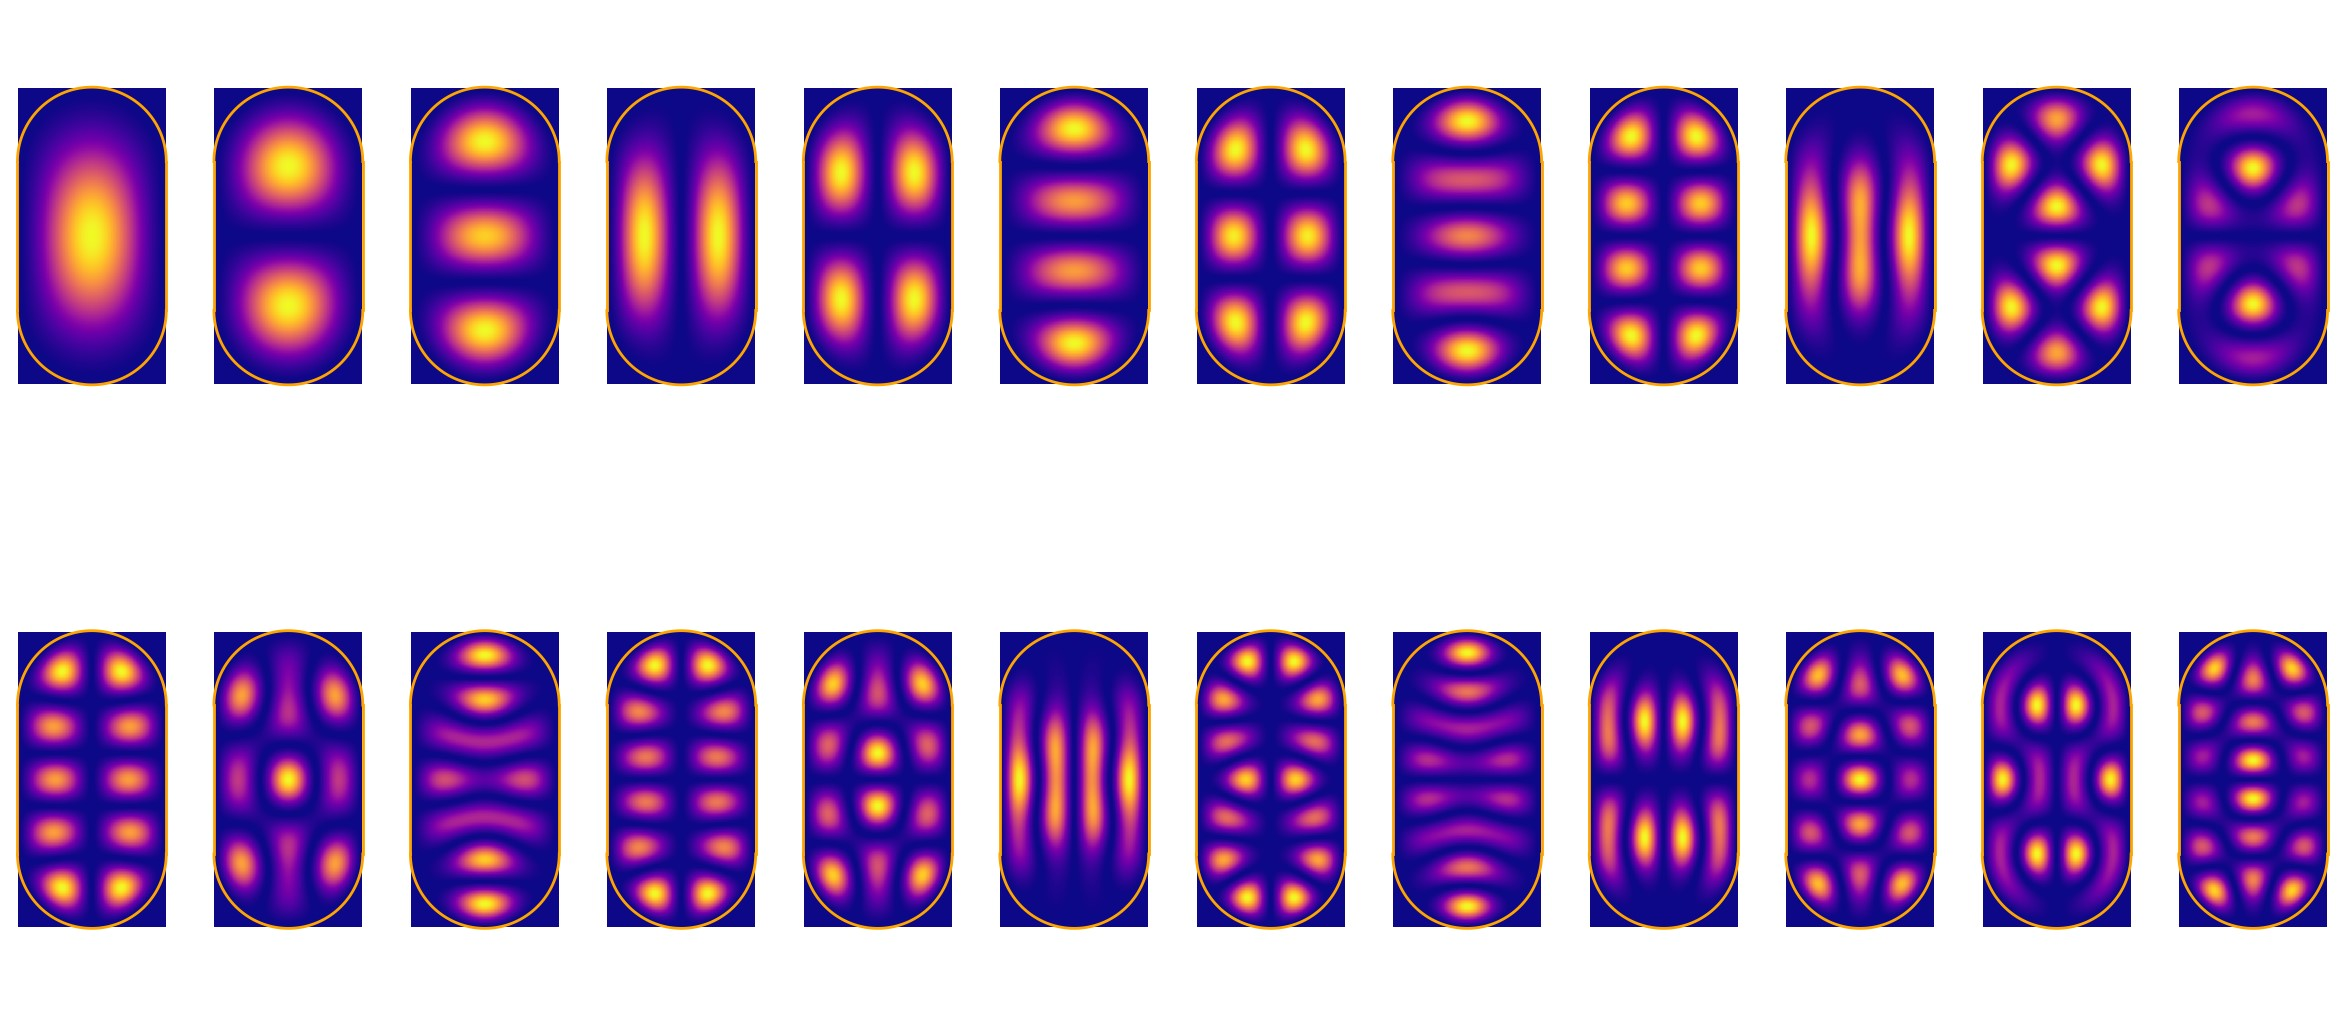
\includegraphics[scale=0.15,angle=0]{quant_stad_24.jpg}
\decoRule
\caption{First 24 eigenfunctions on Bunimovich Stadium}
\label{fig_abstr_eigens}
\end{figure}

\end{abstract}

%----------------------------------------------------------------------------------------
%	ACKNOWLEDGEMENTS
%----------------------------------------------------------------------------------------

\begin{acknowledgements}
\addchaptertocentry{\acknowledgementname} % Add the acknowledgements to the table of contents
The acknowledgments and the people to thank go here\ldots
\end{acknowledgements}

%----------------------------------------------------------------------------------------
%	LIST OF CONTENTS
%----------------------------------------------------------------------------------------

\tableofcontents % Prints the main table of contents

%----------------------------------------------------------------------------------------
%	ABBREVIATIONS
%----------------------------------------------------------------------------------------

\begin{abbreviations}{ll} % Include a list of abbreviations (a table of two columns)

\textbf{LAH} & \textbf{L}ist \textbf{A}bbreviations \textbf{H}ere (TO BE DONE)\\

\end{abbreviations}

%----------------------------------------------------------------------------------------$
%	PHYSICAL CONSTANTS/OTHER DEFINITIONS
%----------------------------------------------------------------------------------------

%\begin{constants}{lr@{${}={}$}l} % The list of physical constants is a three column table
%
%The \SI{}{} command is provided by the siunitx package, see its documentation for instructions on how to use it
%
%Speed of Light & $c_{0}$ & \SI{2.99792458e8}{\meter\per\second} (exact)\\
%%Constant Name & $Symbol$ & $Constant Value$ with units\\
%
%\end{constants} 

%----------------------------------------------------------------------------------------
%	SYMBOLS
%----------------------------------------------------------------------------------------

\begin{symbols}{lll} % Include a list of Symbols (a three column table)

$c$ & light speed & TO BE DONE \\
%Symbol & Name & Unit \\

\addlinespace % Gap to separate the Roman symbols from the Greek

%$\omega$ & angular frequency & \si{\radian} \\

\end{symbols}

%----------------------------------------------------------------------------------------
%	DEDICATION
%----------------------------------------------------------------------------------------

%\dedicatory{Dedicated to\ldots} 
%\thispagestyle{empty}
%----------------------------------------------------------------------------------------
%	THESIS CONTENT - CHAPTERS
%----------------------------------------------------------------------------------------

\mainmatter % Begin numeric (1,2,3...) page numbering

\pagestyle{thesis} % Return the page headers back to the "thesis" style

% Include the chapters of the thesis as separate files from the Chapters folder
% Uncomment the lines as you write the chapters

% Chapter Template

\addchap{Overview} % Main chapter title

\label{Chapter0} % Change X to a consecutive number; for referencing this chapter elsewhere, use \ref{ChapterX}
\thispagestyle{empty}
%----------------------------------------------------------------------------------------
%	SECTION 1
%----------------------------------------------------------------------------------------

\section*{TO BE DONE}
\label{sec:intro}
\addcontentsline{toc}{section}{Main Section 1}%\nameref{sec:intro}}

%\textsf{Description of sections}

\begin{itemize}
\item This chapter;
\item controllare riferimenti tra le varie sezioni;
\item sistemare le appendici;
\item attivare link per folder online con video;
\item fare l'abstract
\item Quantum Cat maps non QUE? Markloff...
\item Inserire (alcuni) programmi nell'appendice
\item Sistemare APPENDICI A e C
\item Accennare meglio agli \emph{scar quantistici}
\end{itemize}





\section{Materials}


All the materials relevant to this thesis, as well with code of numerical simulations, can be found at ATTIVARE LINK
% Chapter Template

\chapter{Billiards and quantum chaos} % Main chapter title

\label{Chapter05} % Change X to a consecutive number; for referencing this chapter elsewhere, use \ref{ChapterX}
\thispagestyle{empty}
%----------------------------------------------------------------------------------------
%	SECTION 1
%----------------------------------------------------------------------------------------

\section{Introduction}
\label{sec:intro}
%\addcontentsline{toc}{section}{Main Section 1}%\nameref{sec:intro}}

%\textsf{E' questo il font}?

The main \virg{physical} dynamical system we will consider in this thesis is a billiard, which is a model where a (usually dimensionless) particle moves within a bounded domain in the Euclidian space $\R^{n}$ and bounces off the boundary of the domain elastically. Physically this can be interpreted in several different ways. But we will also consider the same kind of motion but on surfaces, which will have negative curvature, for reasons that we will learn more about later.\\

The bouncing billiard can be realized, from a physical point of view, by considering, for example, a potential function which zero inside of the considered domain, and equal to infinity otherwise. However, regardless of their physical realization, these kind of system can exhibit a number of interesting properties.

More formally, we will consider the following definition.

\begin{defin}
A \emph{dynamical metric system} is the quadruple $(X,\chi,\mu,R)$ where $(X,\chi,\mu)$ is a metric space with $\sigma$-algebra $\chi$ and $R$ is a $\mu$-measurable map such that $\mu$ is $R$-invariant, i.e. $R_{\ast}\mu=\mu$. 
\end{defin}

Often, $R$ will be more regular than just being measurable. We are now ready to introduce the concept of billiard systems. We will consider essentially, as already mentioned, two main cases:
\begin{itemize}
\item \boldsf{Billiard flows}:\\
A \emph{billiard} is a bounded, planar domain $\Omega$ with a piecewise smooth boundary. The billiard flow is the classical frictionless motion of a particle inside $\Omega$, with angle of incidence to the boundary $\partial\Omega$ equal to angle of reflection off $\partial\Omega$; the total kinetic energy is preserved. In this case, the preserved measure is a multiple of Lebesgue measure, i.e. Liouville measure, given explicity by $\mu_{L}=\frac{\one_{\Omega}}{\lambda(\Omega)}$, where $\lambda(\Omega)$ is the measure of set $\Omega$. If we consider the unit tangent space $T^{1}\Omega$, then the Liouville measure is given by $\mu_{L}=\frac{\one_{\Omega}}{2\pi\lambda(\Omega)}$. 
\item \boldsf{Geodesic flows (on manifolds)}:\\
If $M$ is a Riemannian manifold with metric $g$, then for each point $q\in M$, there is one and only one \emph{geodesic} (i.e. path of minimal length) given a unit direction. So the classical frictionless motion of a particle along local geodesics gives the desired flow. Moreover, it's well defined the unit tangent space $T^{1}M$ and in this case the Liouville measure is given by $\mu_{L}=\frac{\one}{2\pi\lambda(M)}$ where $\lambda(M)$ is the \virg{area} of $M$, with respect to metric $g$. 
\end{itemize}
In both cases, we will denote the considered flow with $\Phi_{t}$. Sometimes, it is more convenient to consider only a \emph{discretization} of the flow; for example, in billiard flow case, it can be helpful to consider the map $\Psi=\Phi_{T}^{n}$ which gives the position of a point $q\in\Omega$ after time $nT$.\\
Billiards systems, even if simple in their definition, can exhibit a certain degree of \emph{chaotical properties}. A good property to look at for this type of features is ergodicity.

\begin{nteo}[Ergodicity, discrete case]
\label{definteo:ergodic_discrete}
Let $(X,\chi,\mu,R)$ be a dynamical metric system, with $X$ of finite measure, i.e. a probability space. The followings hold and give a definition of a (discrete) ergodic system:
\begin{compactitem}
\item if $B$ is $R$-invariant, then $\mu(B)=0$ or $\mu(B^{\compl})=0$
\item if $\mu(A),\mu(B)>0$ for measurable sets $A,B$, then it does exist a $k\geq0$ such that $\mu(A\cap R^{-k}[B])>0$.
\end{compactitem}
\end{nteo}

Roughly speaking, ergodicity requires that a dynamical system cannot be decomposed in smaller and indipendent dynamical system and every set is taken across all the space $X$ through the action of map $R^{-k}$, with $k\geq0$. Moreover, every subset $A$ must be \virg{mixed} with every other subset $B$, in a certain proportion. In fact, another important feature is the concept of \emph{mixing}. 

\begin{defin}[Mixing]
\label{defin:mixing_discrete}
A dynamical metric system $(X,\chi,\mu,R)$ is called \emph{mixing} if $\,\forall A,B\in\chi$ we have
\[
\lim_{n\to\infty}\abs{\mu(A\cap R^{-n}[B])-\mu(A)\mu(B)}=0.
\]
\end{defin}

Mixing is indeed a \underline{stronger property} than ergodicity, because it does not only require that the system mixes itself, but every couple of sets $A,B$ should be mixed in \emph{the right proportion}.\\
We can rewrite these definition for the continuos case.

\begin{defin}[Ergodicity and mixing, continuos case]
\label{defin:ergodic_mixing_contin}
Let $(X,\chi,\mu,\Phi_{t})$ be a dynamical metric system, with $X$ of finite measure, i.e. a probability space.
\begin{compactitem}
\item The flow $\Phi_{t}$ is \emph{ergodic} if for every measurable set $B\subset X$ which is $R_{t}$ invariant for every $t$, then $\mu(B)=0$ or $\mu(B^{\compl})=0$;
\item The flow $\Phi_{t}$ is \emph{mixing} if for every measurable sets $A,B\subset X$
\[
\mu(A\cap\Phi_{t}^{-1}[B])\stackrel{t\to\infty}{\longrightarrow}\mu(A)\mu(B).
\]
\end{compactitem}
\end{defin}

A more pictorial way to understand ergodicity from a physical point of view is given by the following result, due to Birkhoff.

\begin{nteo}[Birkhoff]
\label{teo:birkhoff}
The flow $\Phi_{t}$ is ergodic iff $\forall f\in L^{1}(X)$,
\[
\lim_{T\to\infty}\frac{1}{T}\int_{0}^{T}f\circ\Phi_{t}(x)\dd t = \int_{X}\vphi \dd\mu
\]
for $\mu$-a.e. $x\in X$.
\end{nteo}

What theorem \ref{teo:birkhoff} states is that, in an ergodic system, the trajectories are equidistributed in the phase space. There is also a reinterpretation of ergodicity from a \virg{spectral} point of view, considering the precomposing map $R^{\ast}f=f\circ R$.

\begin{nteo}
\label{teo:ergodic_spectral} 
Let $(X,\chi,\mu,R)$ be a metric system e let $p\in[1,+\infty]$. The followings are equivalent:
\begin{compactitem}
\item the system $(X,\chi,\mu,R)$ is ergodic;
\item the eigenspace of $R^{\ast}$ in $L_{p}$ corrispondent to eigenvalue $1$ is made up only by a.e. constant functions $\mathbb{C}\one$.
\end{compactitem}
\end{nteo}

We will go deeper into this \virg{spectral} approach in the following chapters.


\subsection{Examples}

We are now ready to analyze some examples. At first, we will consider some classical billiards.\\[2mm]

\noindent{\large \boldsf{Billiards}}:

\begin{nese}[Biliardo circolare, ellittico]
The circular, elliptic billiard is given by the classical \virg{bouncing motion} and a domain $\Omega\subset\R^{2}$ which is given by a circle or, more generally, an ellipse. In this case, the billiard \underline{is not ergodic}, as it can be easy seen in the circular case. In fact, if the angle of first bounce is $\vtheta$, then for the symmetry of the circle, this angle is constant through every bounce and so it is a constant quantity over an orbit and depending on the considered orbit. So, for theorem \ref{teo:ergodic_spectral}, this system cannot be ergodic. This property has a concrete impact on the aspect of a generic orbit. Seeing figure \ref{fig:ell_circ_billiards}, it can be observed that a generic orbit avoids whole parts of the domain.  
\end{nese}


\begin{figure}[H]
\centering
  \begin{subfigure}[b]{0.3\textwidth}
  \centering
    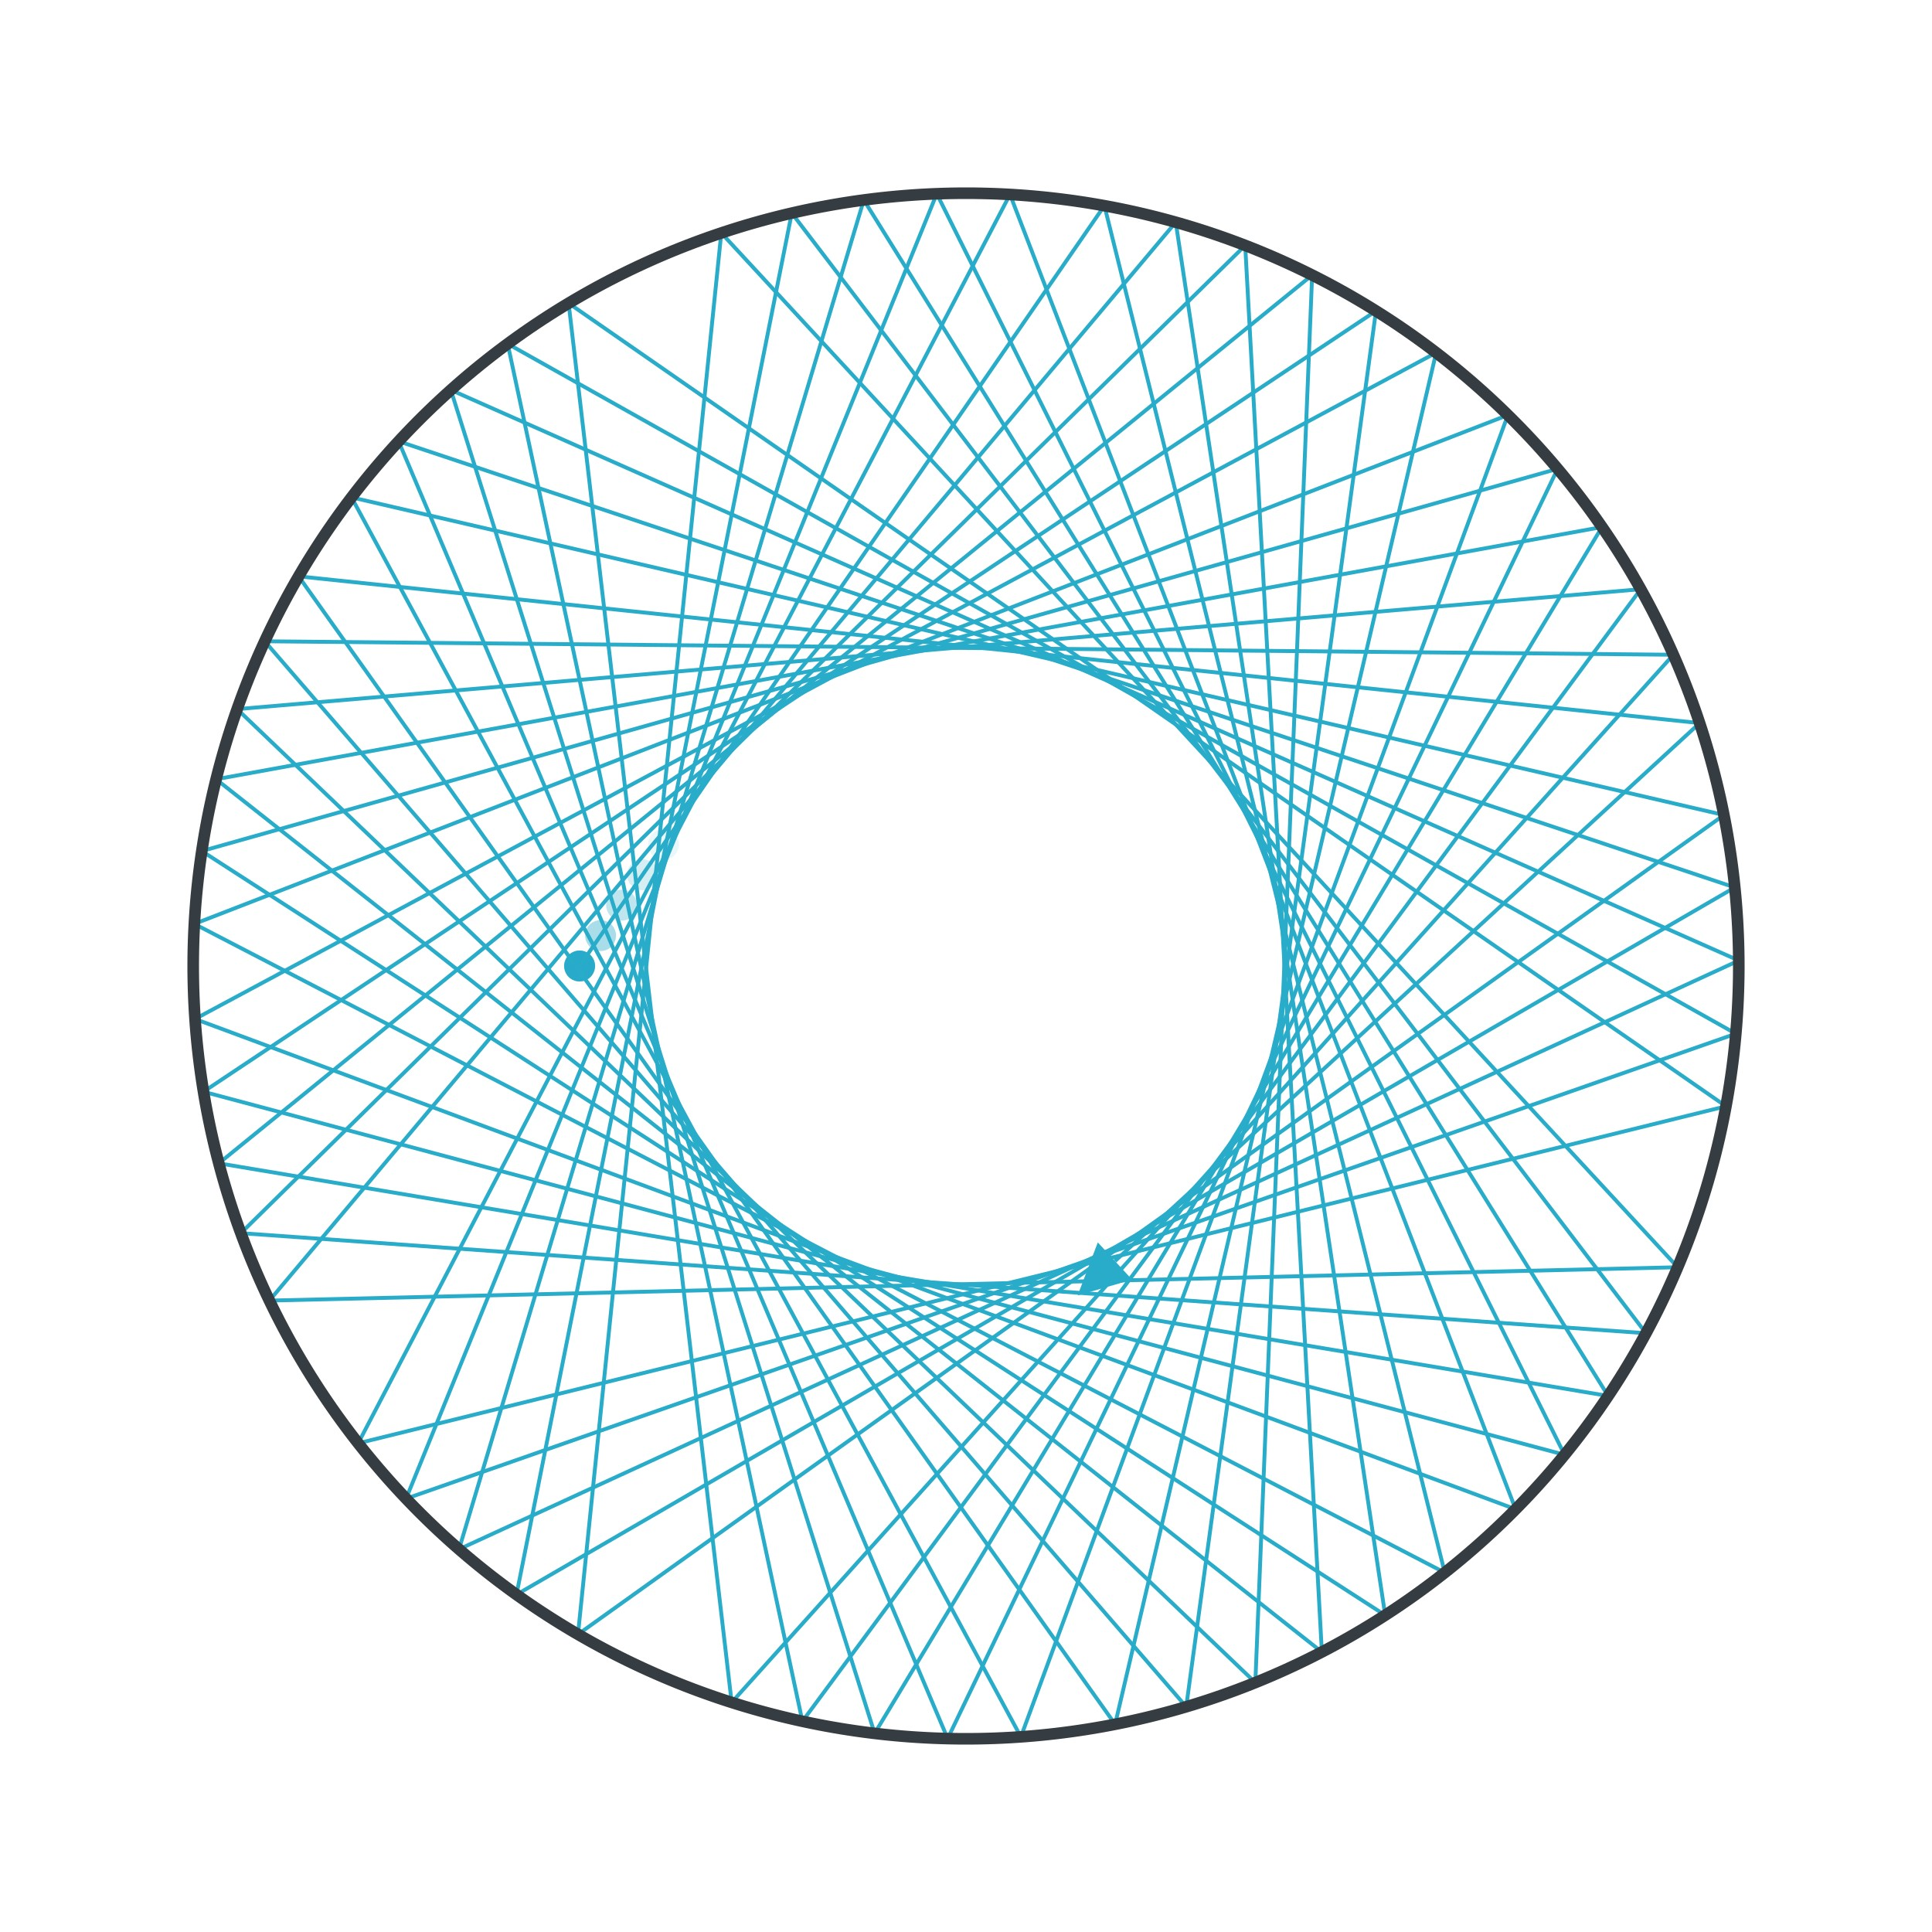
\includegraphics[scale=0.04,angle=0]{Circle_2.jpg}
    %\caption{Variabili $X_{n}$}
    \label{fig:circ1}
  \end{subfigure}
  %
  \begin{subfigure}[b]{0.3\textwidth}
  \centering
    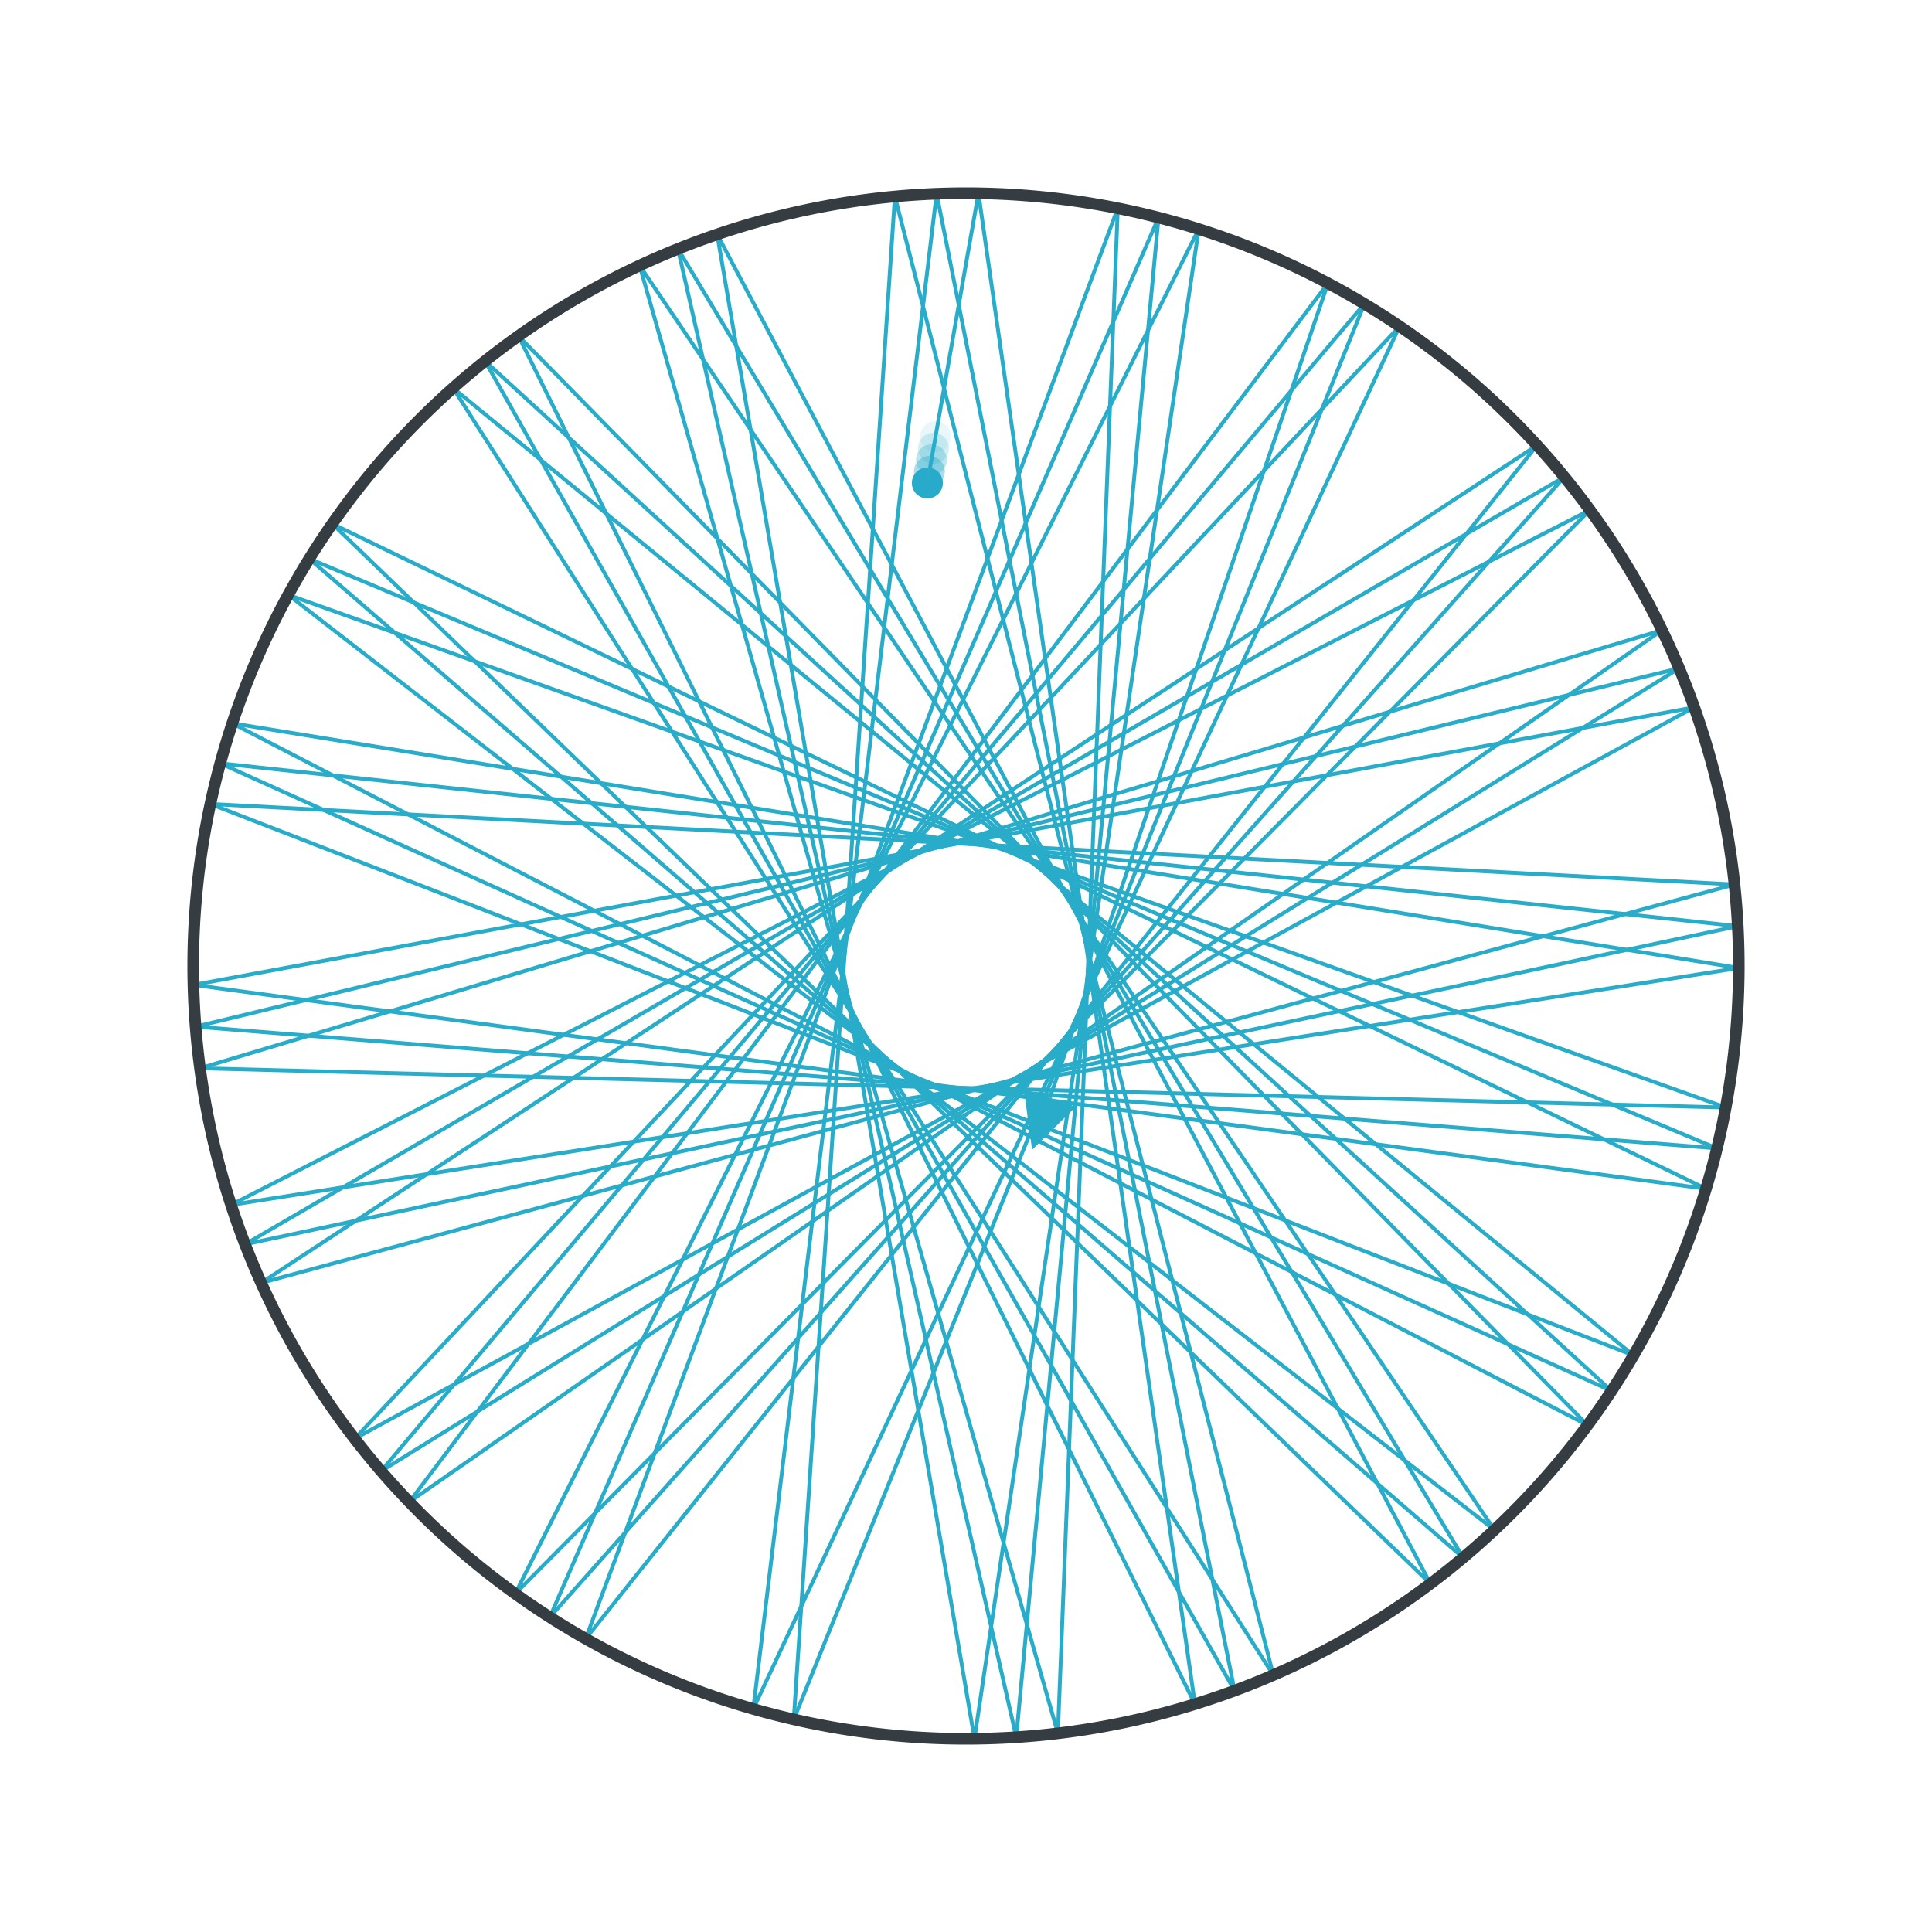
\includegraphics[scale=0.04,angle=0]{Circle_3.jpg}
    %\caption{Variabili $X_{n}$}
    \label{fig:circ2}
  \end{subfigure}
  \begin{subfigure}[b]{0.3\textwidth}
  \centering
    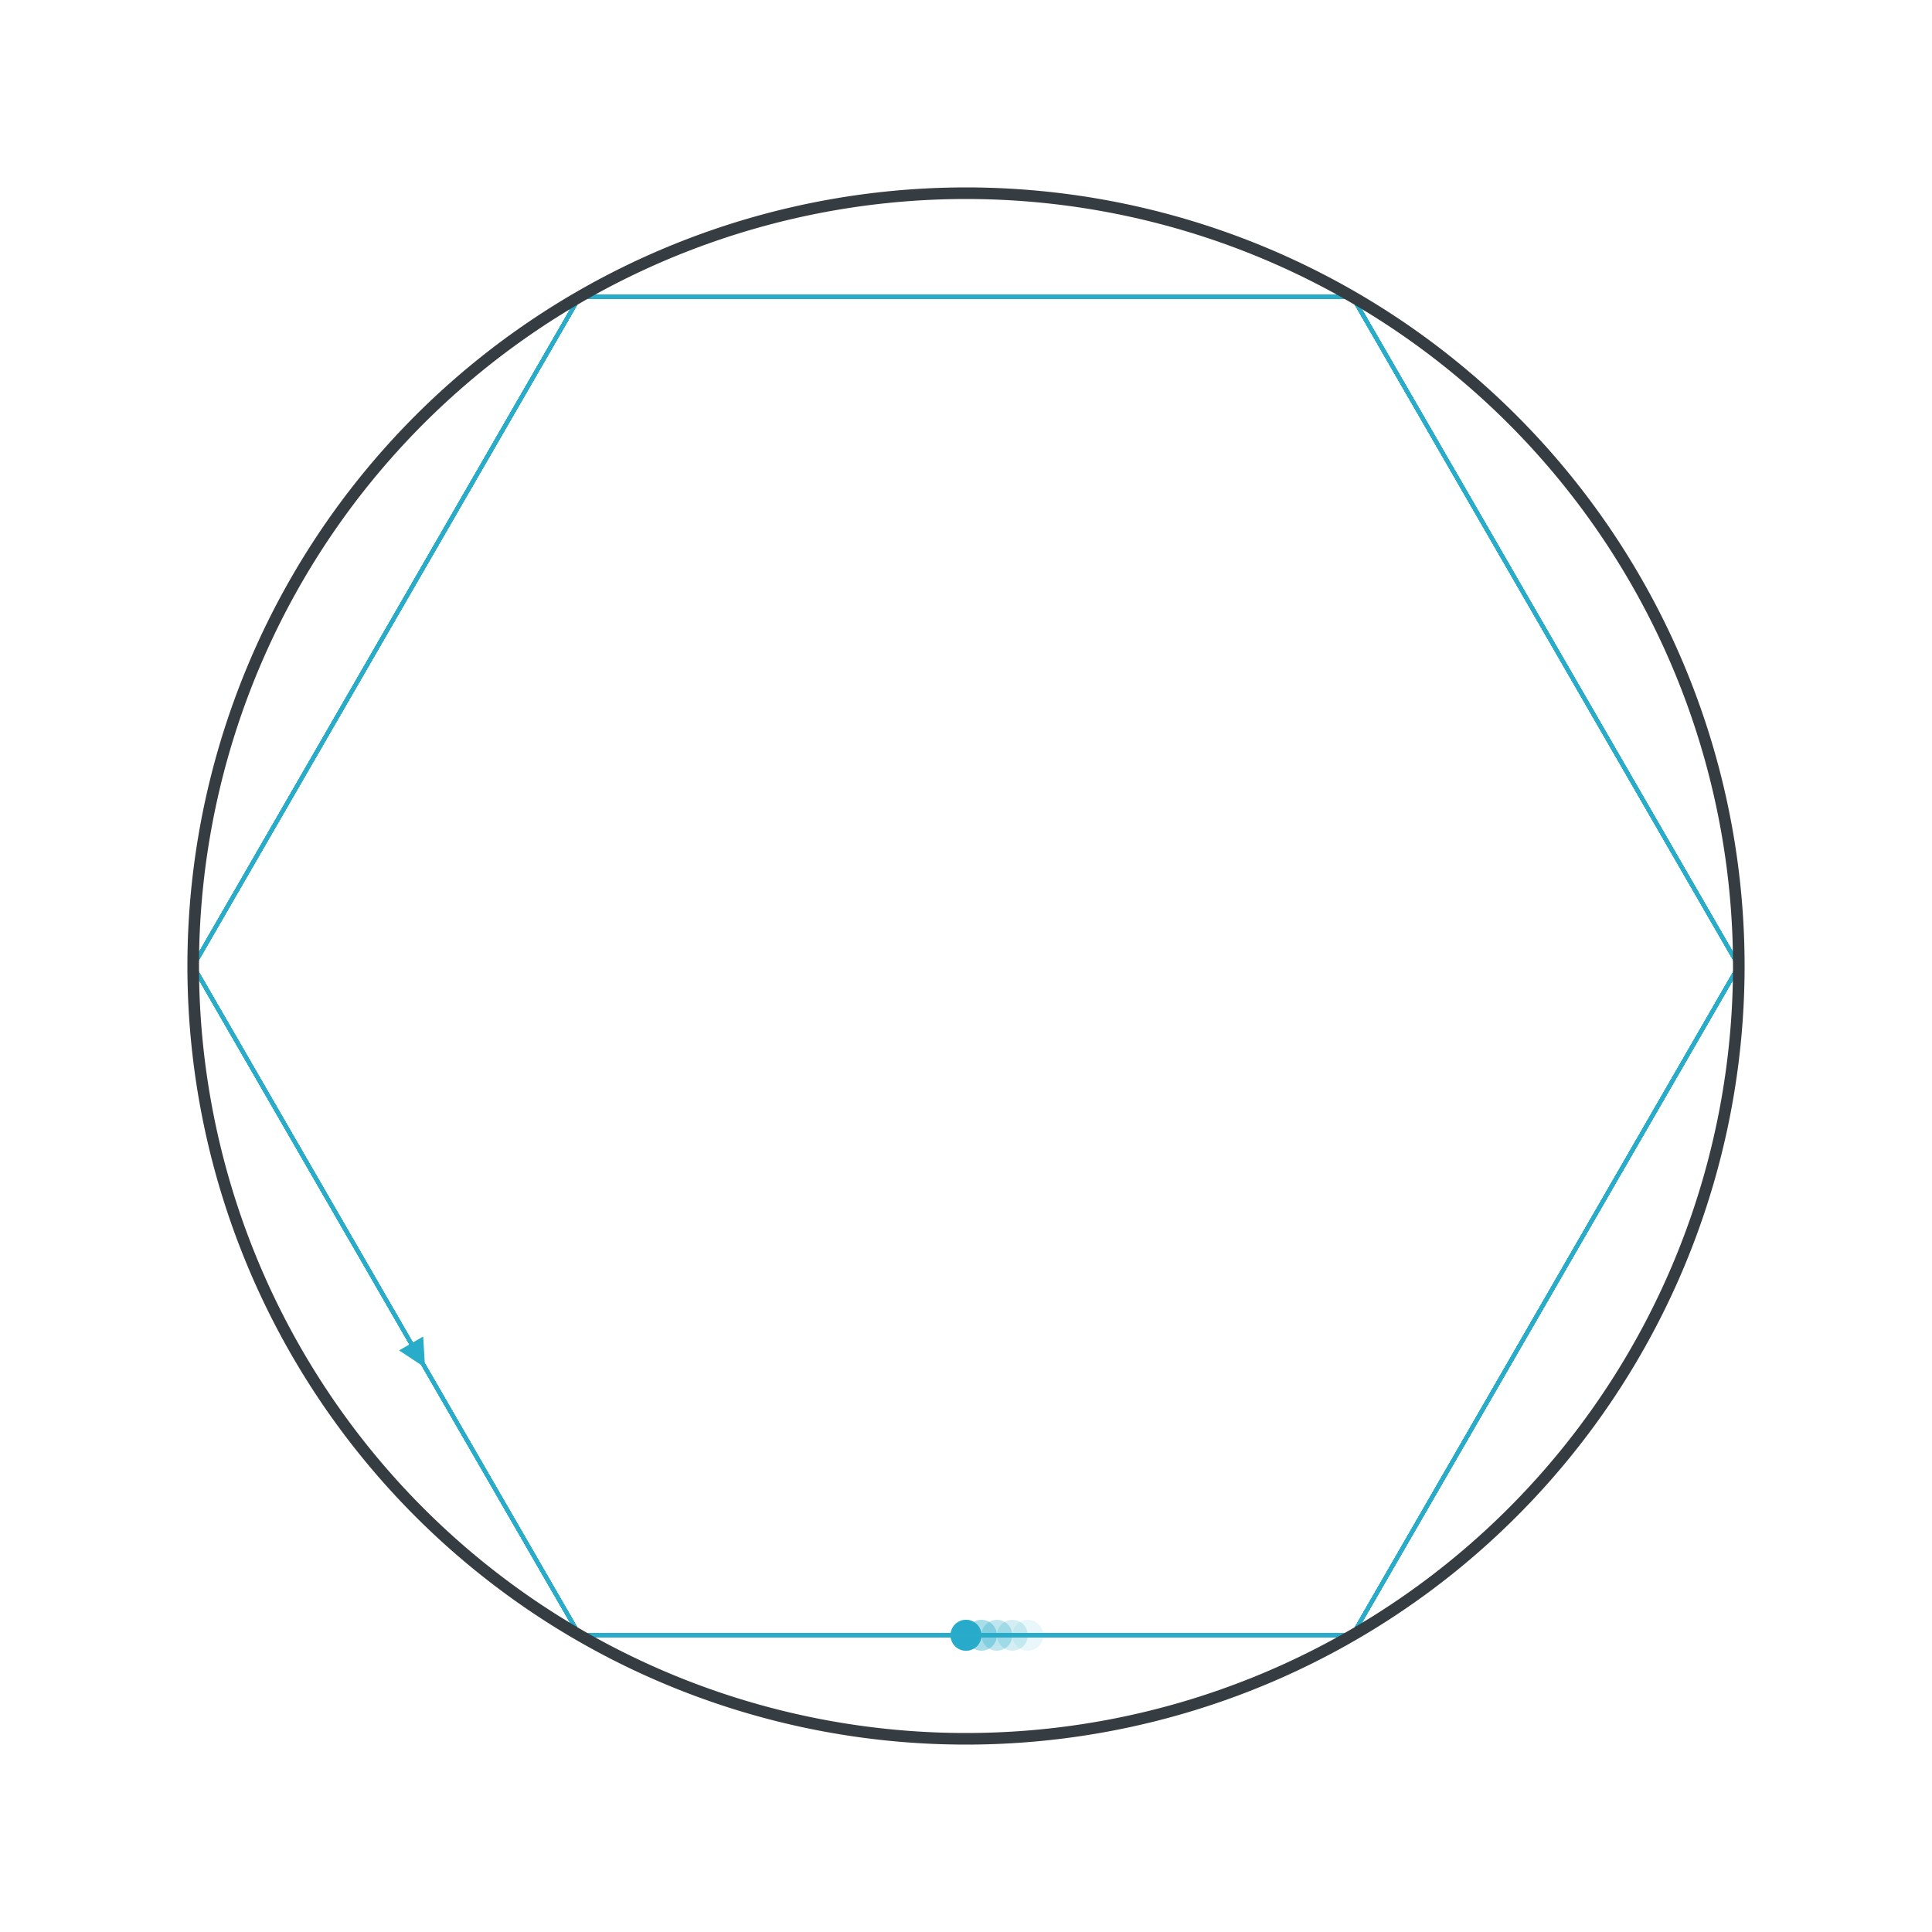
\includegraphics[scale=0.04,angle=0]{Circle_4.jpg}
    %\caption{Variabili $X_{n}$}
    \label{fig:circ3}
  \end{subfigure}
  \noindent\\
  \begin{subfigure}[b]{0.4\textwidth}
  \centering
    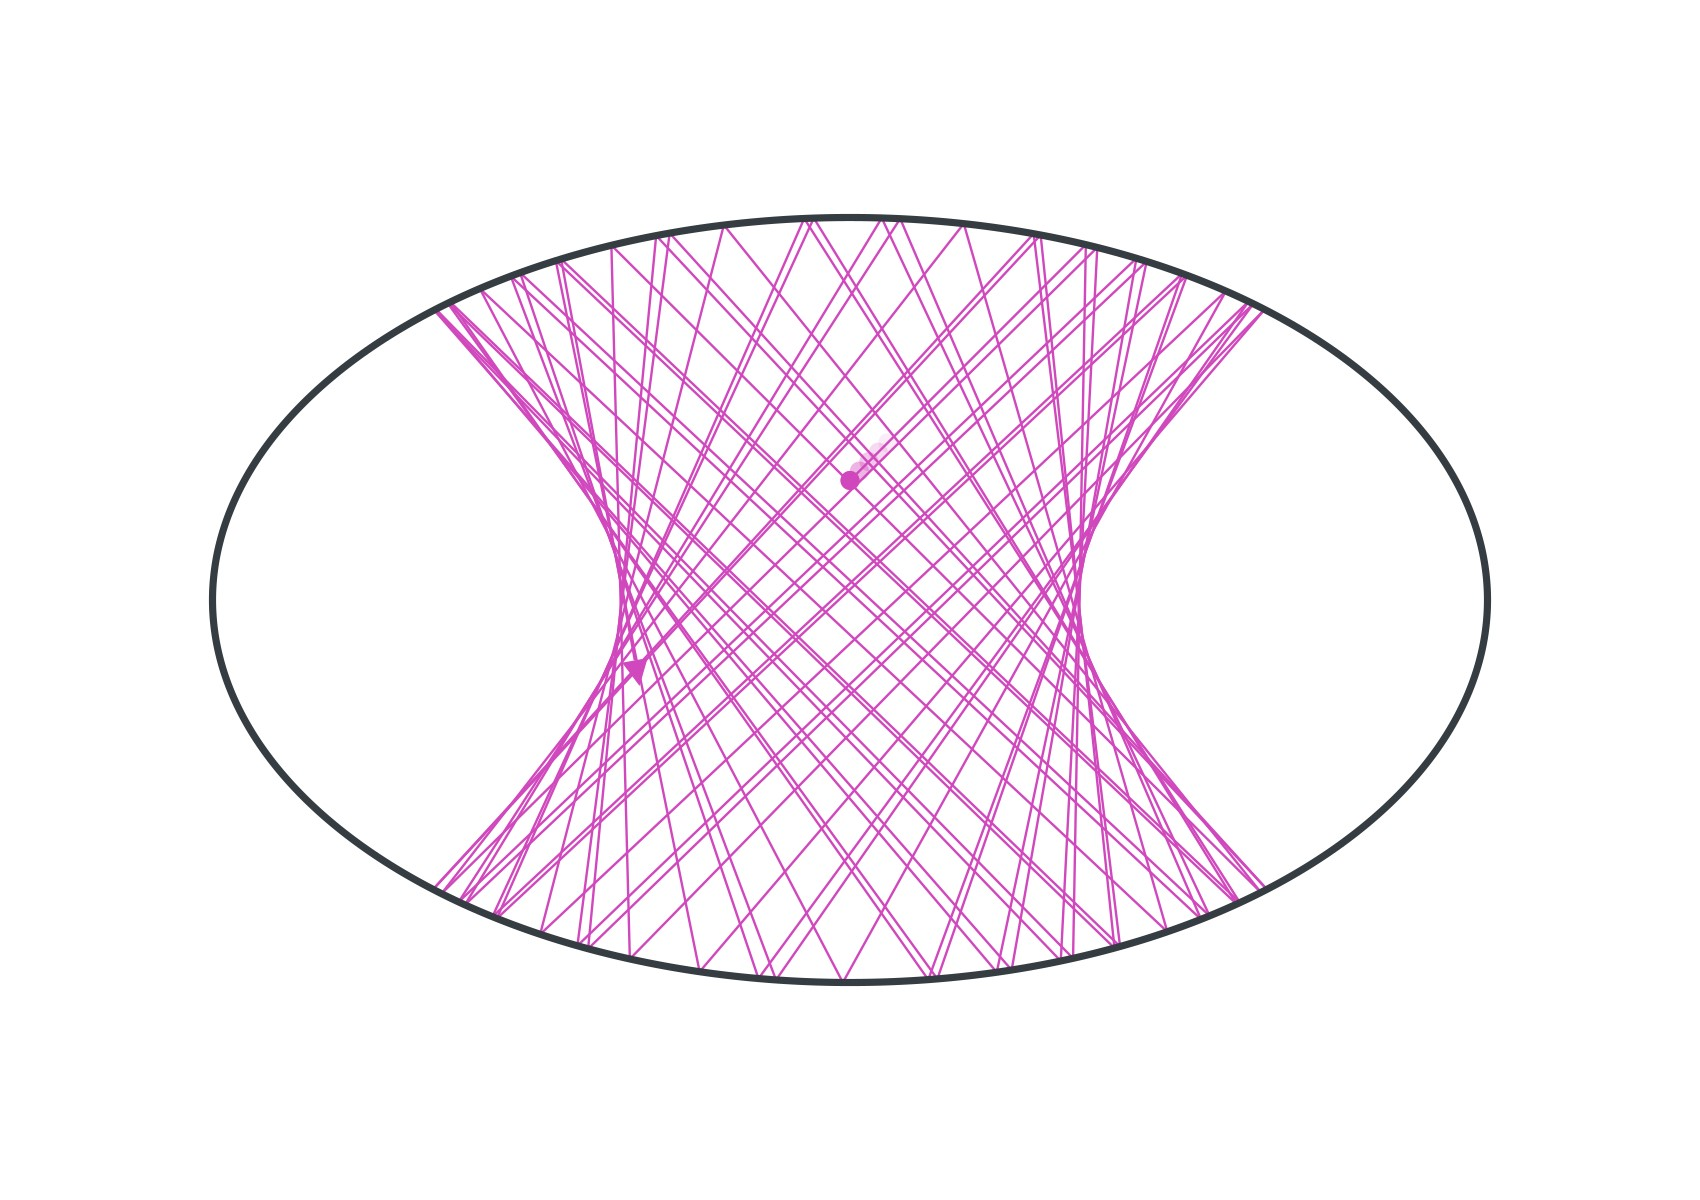
\includegraphics[scale=0.08,angle=0]{Ellipse1.jpg}
    %\caption{Variabili $X_{n}$}
    \label{fig:ellip1}
  \end{subfigure}
  \begin{subfigure}[b]{0.4\textwidth}
  \centering
    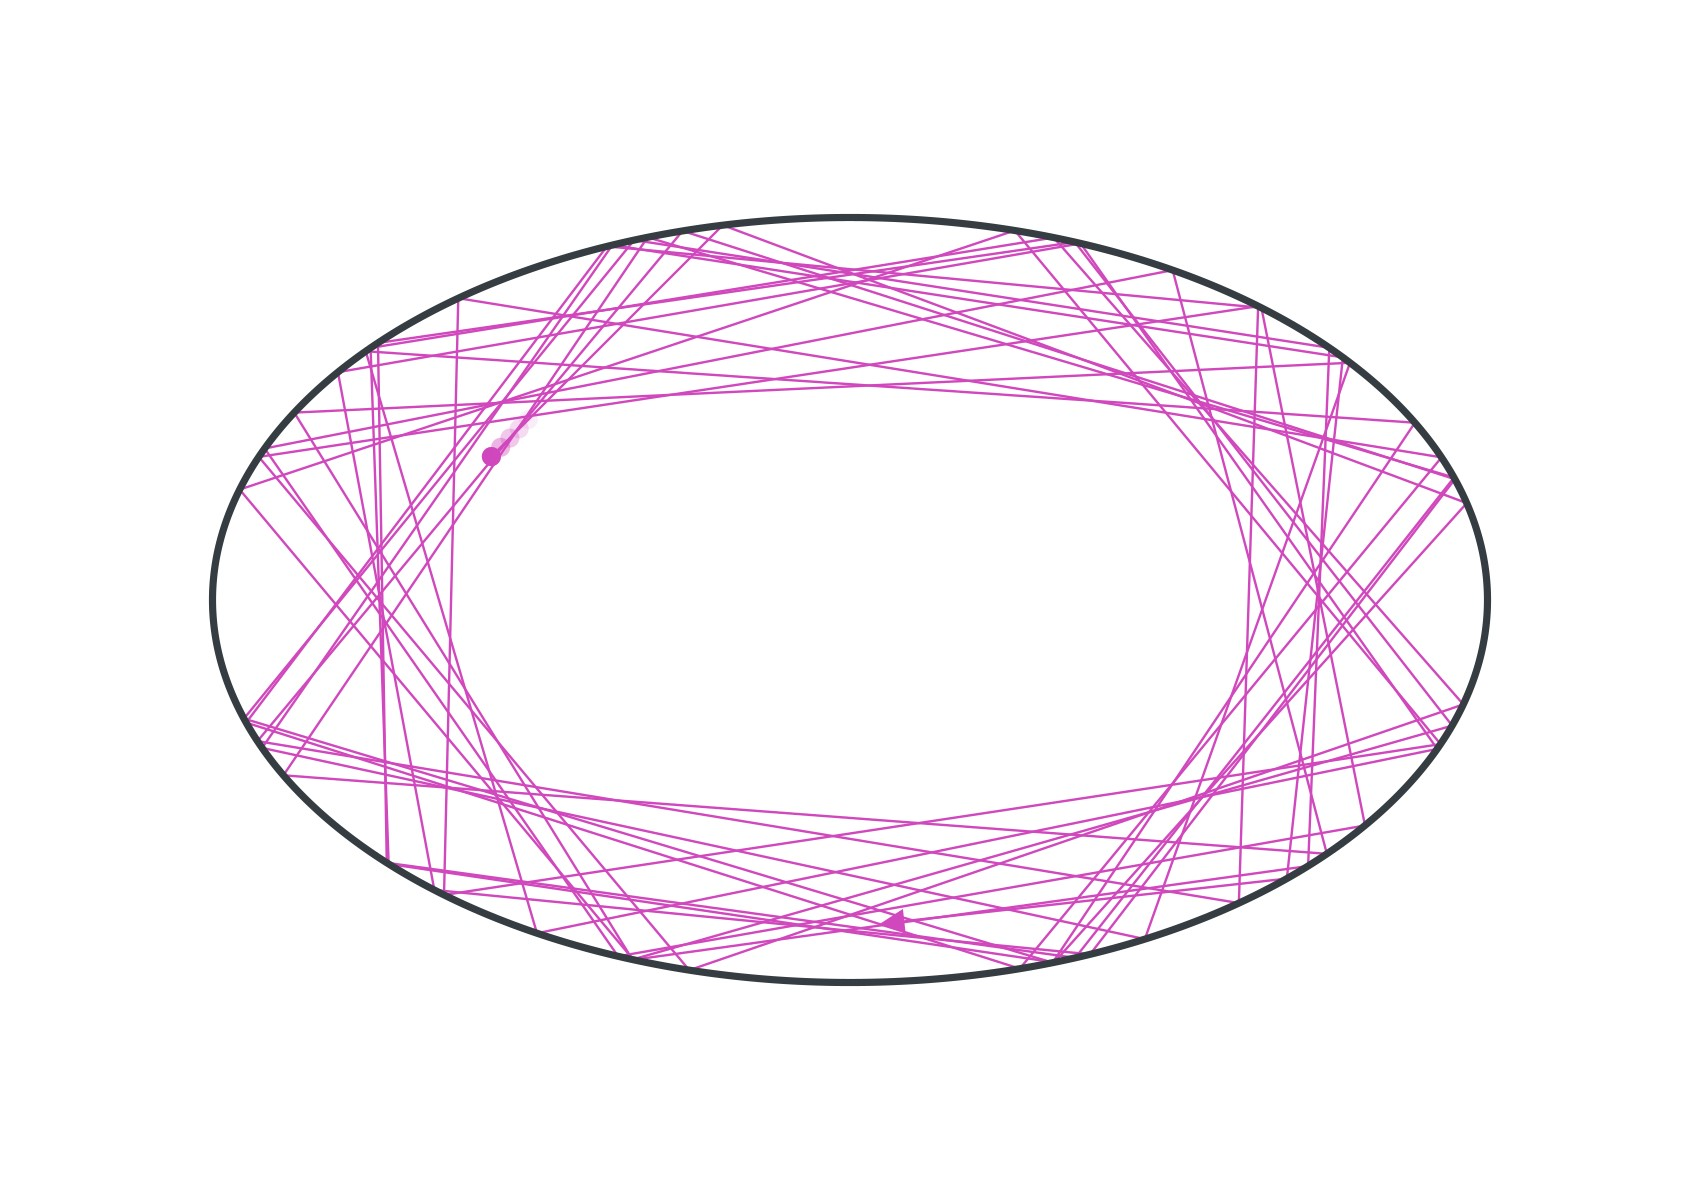
\includegraphics[scale=0.08,angle=0]{Ellipse2.jpg}
    %\caption{Variabili $X_{n}$}
    \label{fig:ellip2}
  \end{subfigure}
  \noindent\\
  \decoRule
  \caption{Billiard trajectories on a circle and an ellipse. The underlying system is conservative, hence the motion is not \virg{everywhere distributed}.}
  \label{fig:ell_circ_billiards}
\end{figure}


The followings are examples of ergodic billiards.

\begin{nese}[Bunimovich stadium]
\label{ese:bunimovich_stadium}
This billard is by far the most famous one and the most studied in details. Albeit it may seem contrived, this billiard is full of remarkable properties and so it is considered the fundamental prototype for a chaotic billiard. The domain $\Omega$ is made up by one rectangle and two half-circles on two sides. This billiard is ergodic and mixing. Moreover, it is also \virg{chaotic} in the sense that \virg{near trajectories} have drammatically different time-evolution (see figure \ref{fig:bunimovich_orbits})\\
We will denote by $\BS_{l}$ the Bunimovich stadium defined by the rectangle $\left[
-l\frac{\pi}{2},l\frac{\pi}{2}
\right]\times
\left[
-\frac{\pi}{2},\frac{\pi}{2}
\right]$ and the two semicircle of radius $\pi/2$.
\end{nese}


\begin{figure}[H]
\centering
  \begin{subfigure}[b]{0.7\textwidth}
  \centering
    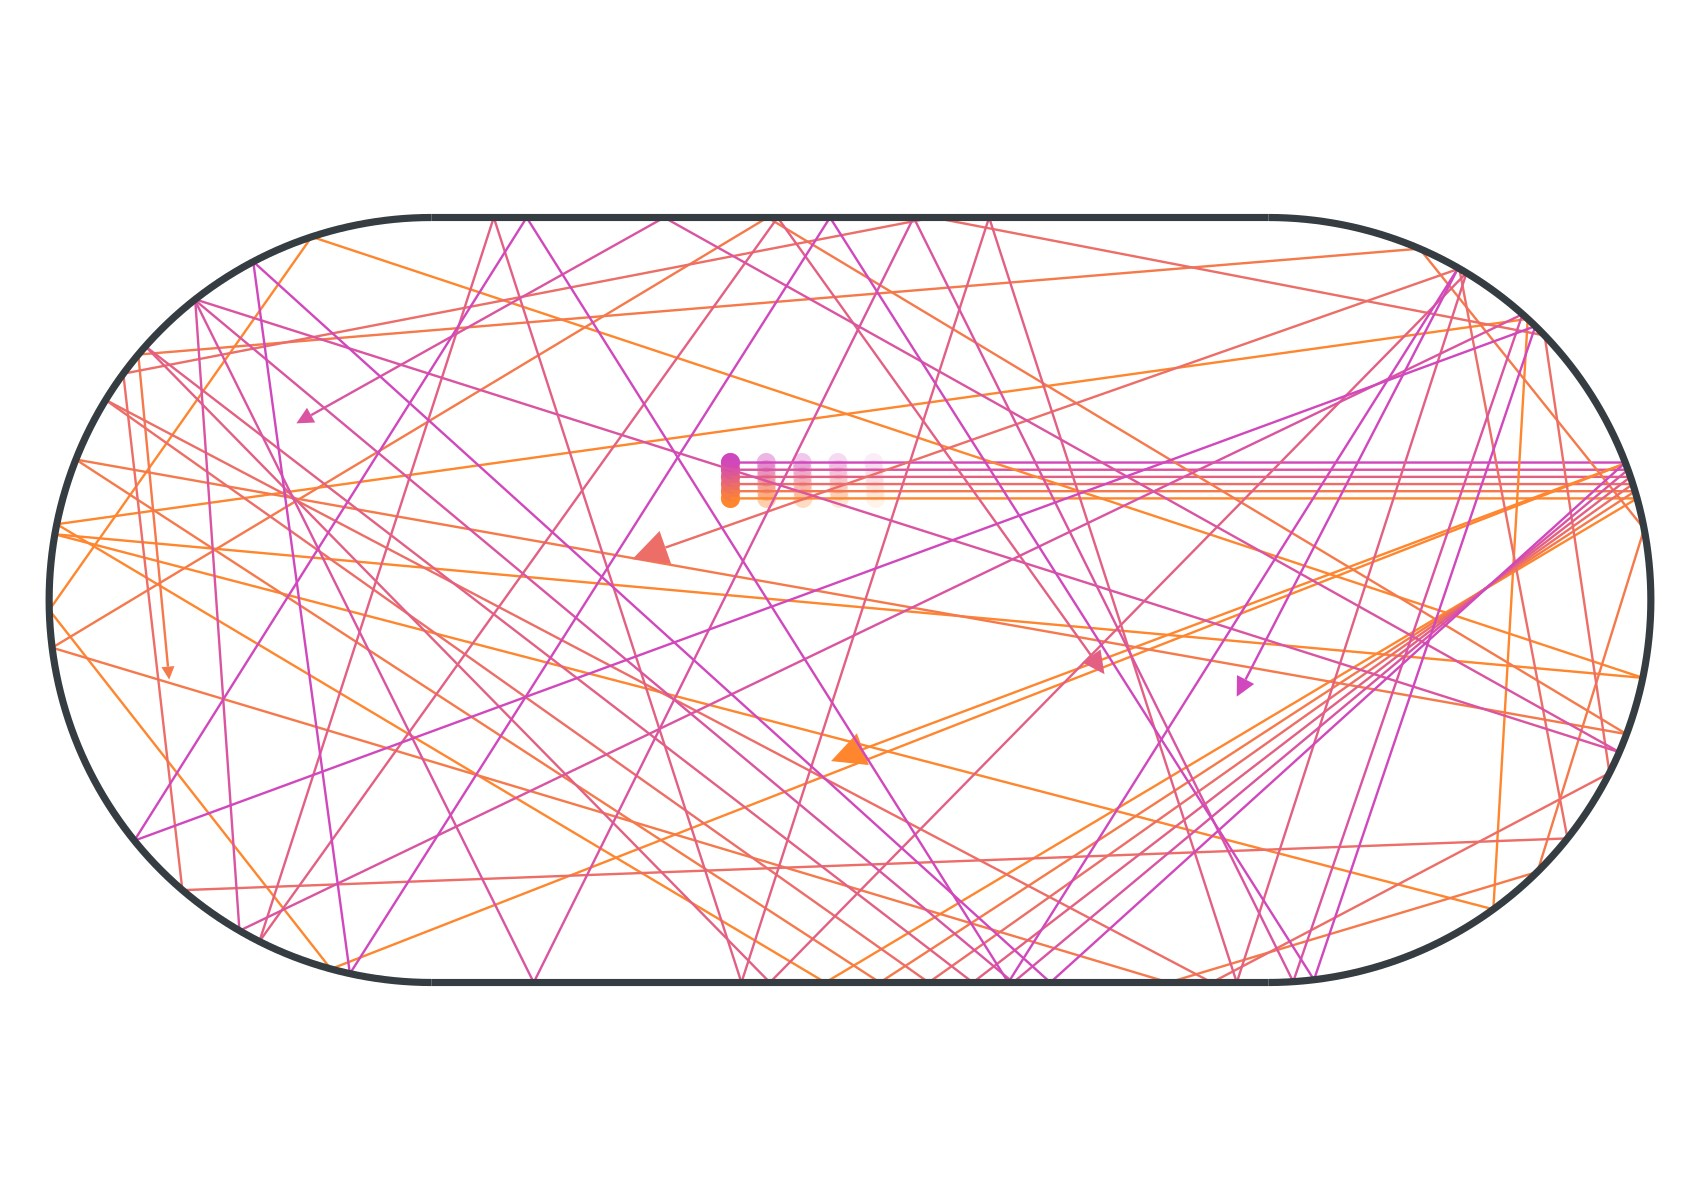
\includegraphics[scale=0.11,angle=0]{Stadium_diverg.jpg}
    %\caption{Variabili $X_{n}$}
    \label{fig:bun1}
  \end{subfigure}
  %
  \noindent\\
  \begin{subfigure}[b]{0.3\textwidth}
  \centering
    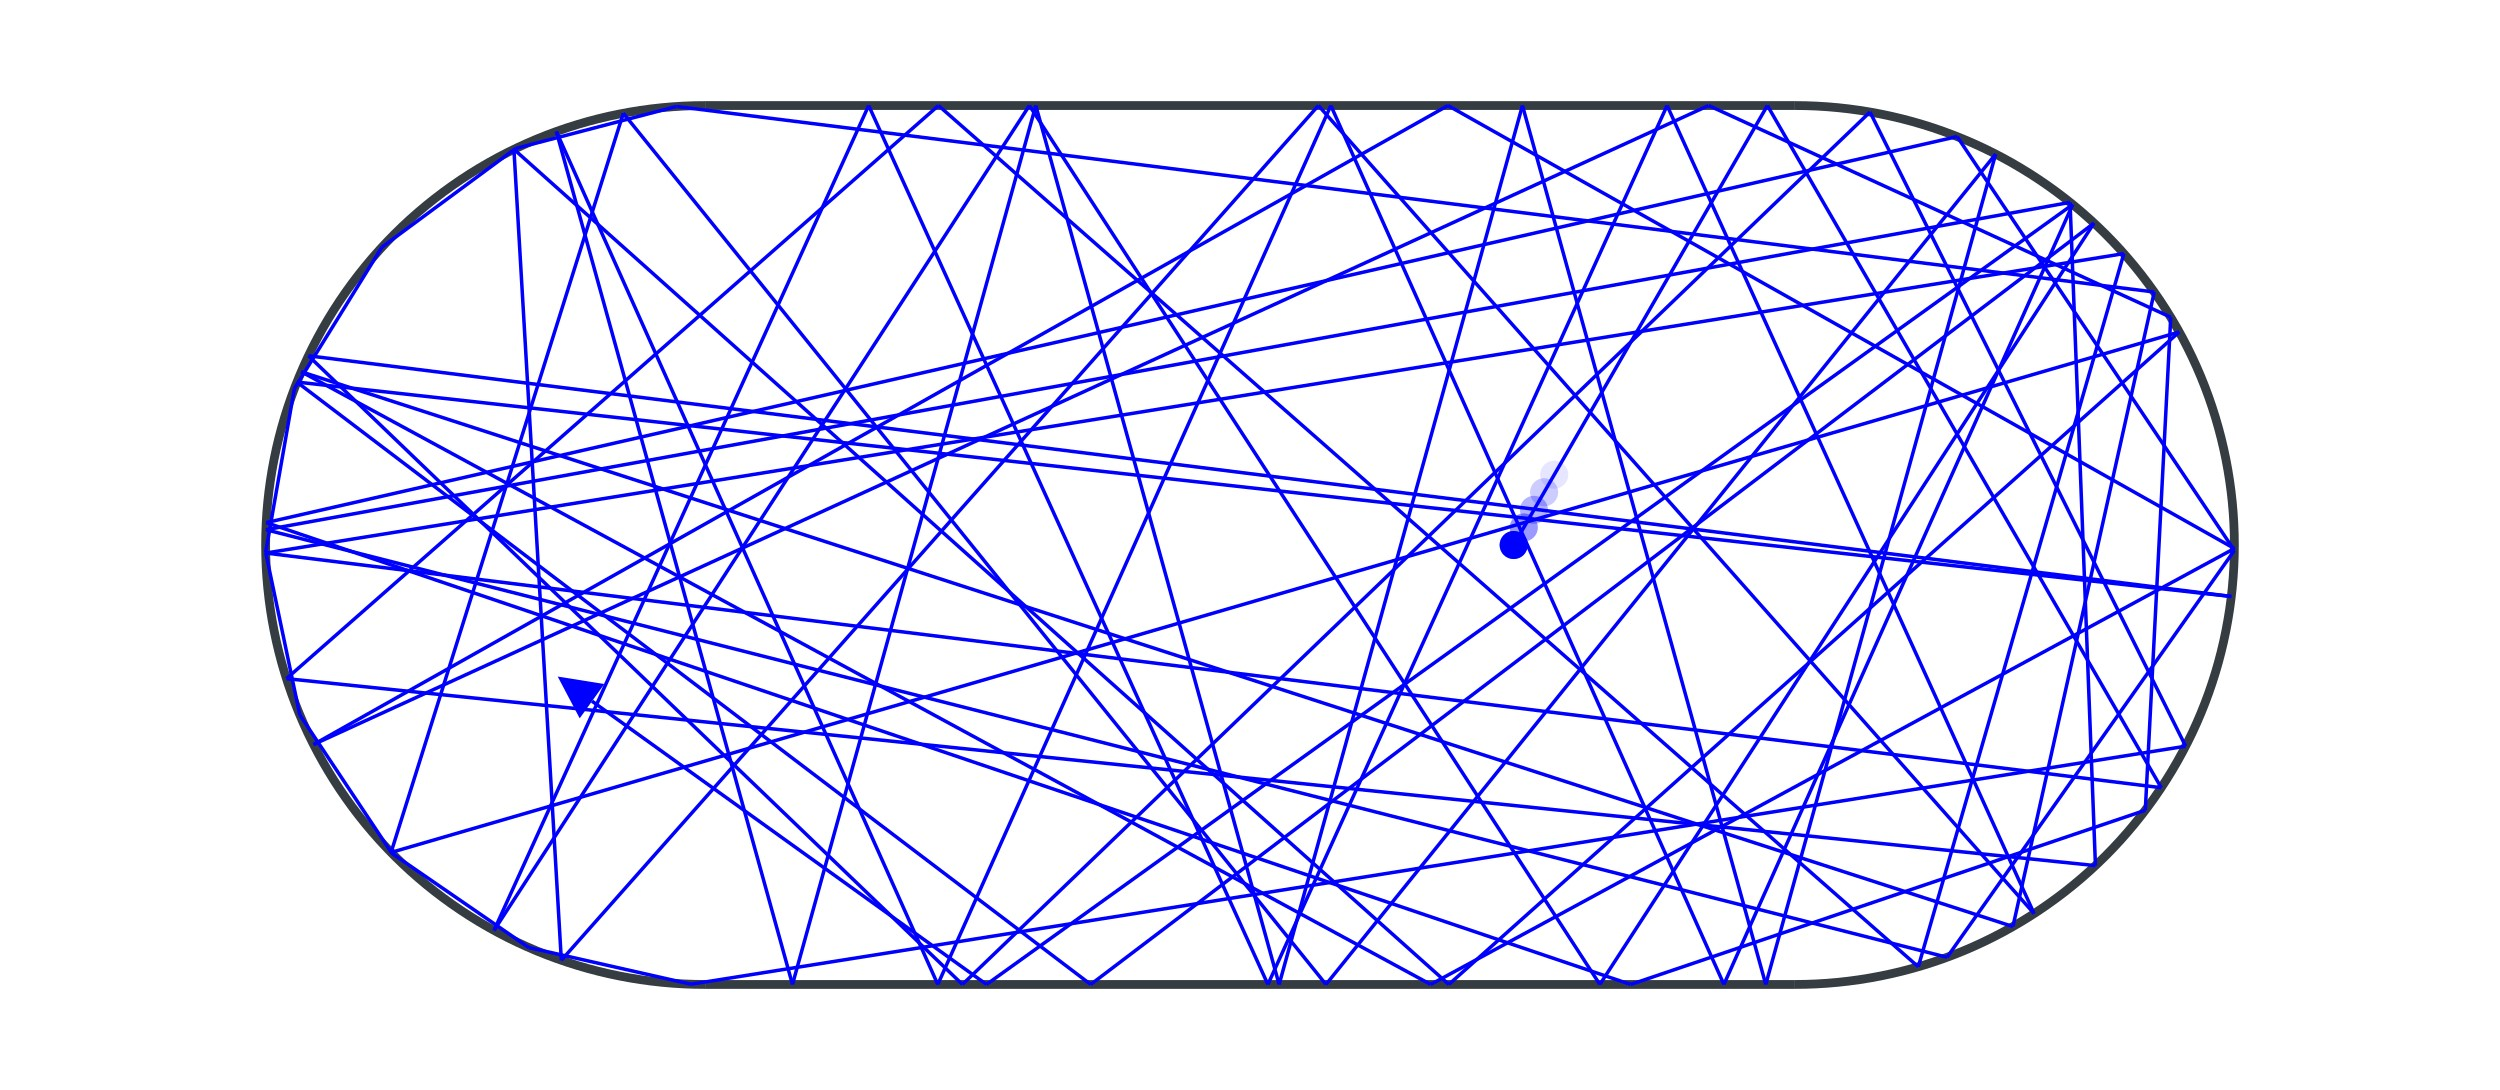
\includegraphics[scale=0.05,angle=0]{Stad_2.jpg}
    %\caption{Variabili $X_{n}$}
    \label{fig:bun2}
  \end{subfigure}
  \begin{subfigure}[b]{0.3\textwidth}
  \centering
    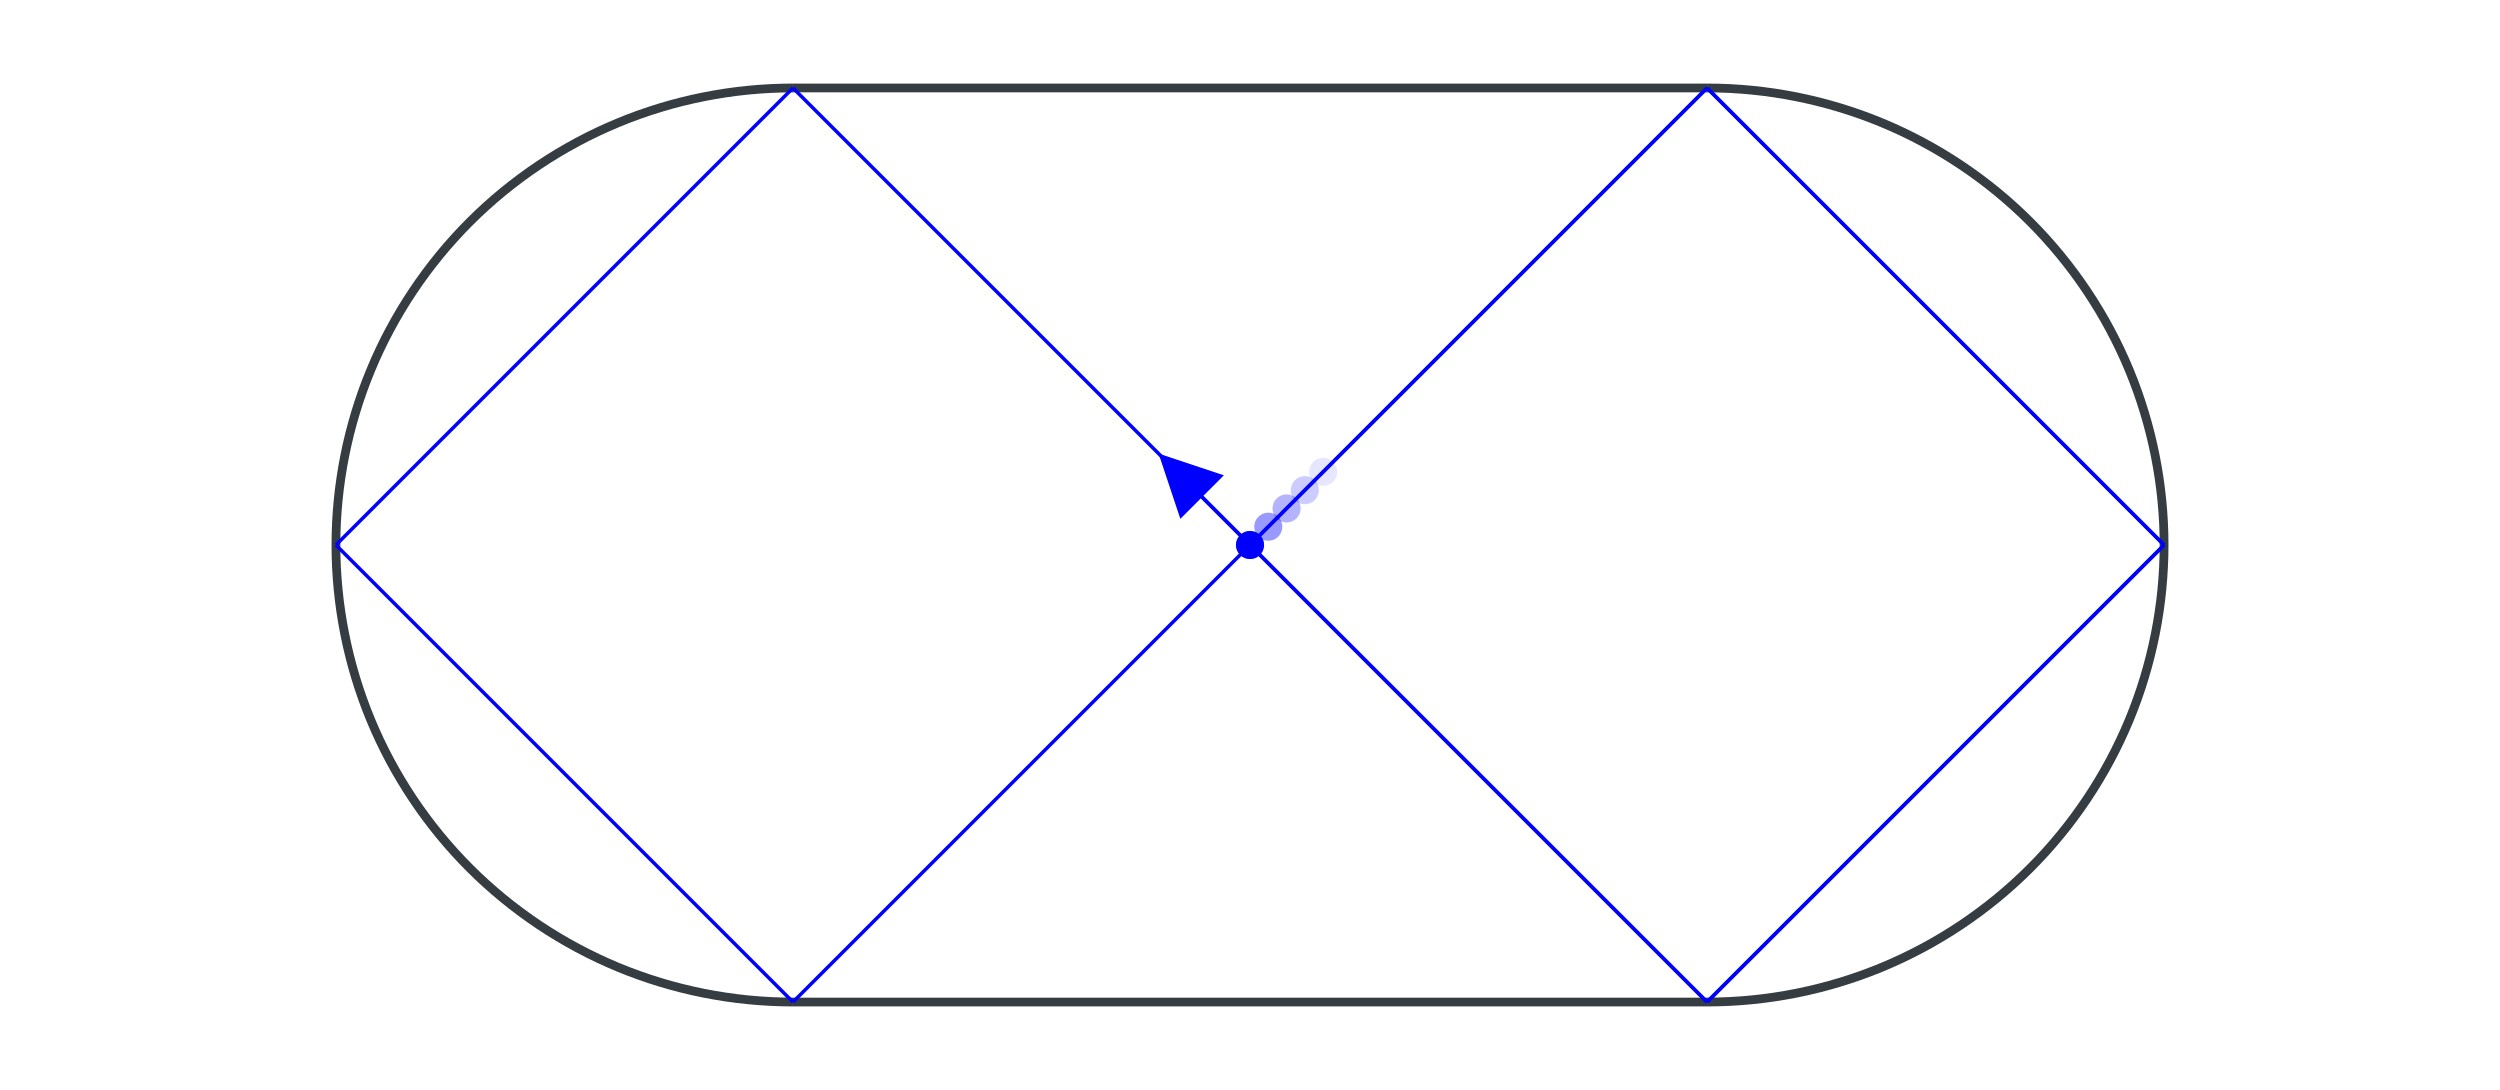
\includegraphics[scale=0.05,angle=0]{Stad_3.jpg}
    %\caption{Variabili $X_{n}$}
    \label{fig:bun3}
  \end{subfigure}
  \noindent\\
  \decoRule
  \caption{Billiard trajectories on the Bunimovich stadium.}
  \label{fig:bunimovich_orbits}
\end{figure}


\begin{nese}[Barnett's billiard]
This billiard is made up by two circle arcs and two perpendicular segment. The circle arcs must intersect creating an acute angle. Peter Sarnak called this billiard \virg{Barnett's billiard}, thanks to the latter's numerical studies on this billiard. We will denote the generic Barnett's billiard with $\BarS$. It is mixing and, moreover, Sinai proved that near orbits diverge exponentially.
\end{nese}


\begin{figure}[H]
\centering
  \begin{subfigure}[b]{0.7\textwidth}
  \centering
    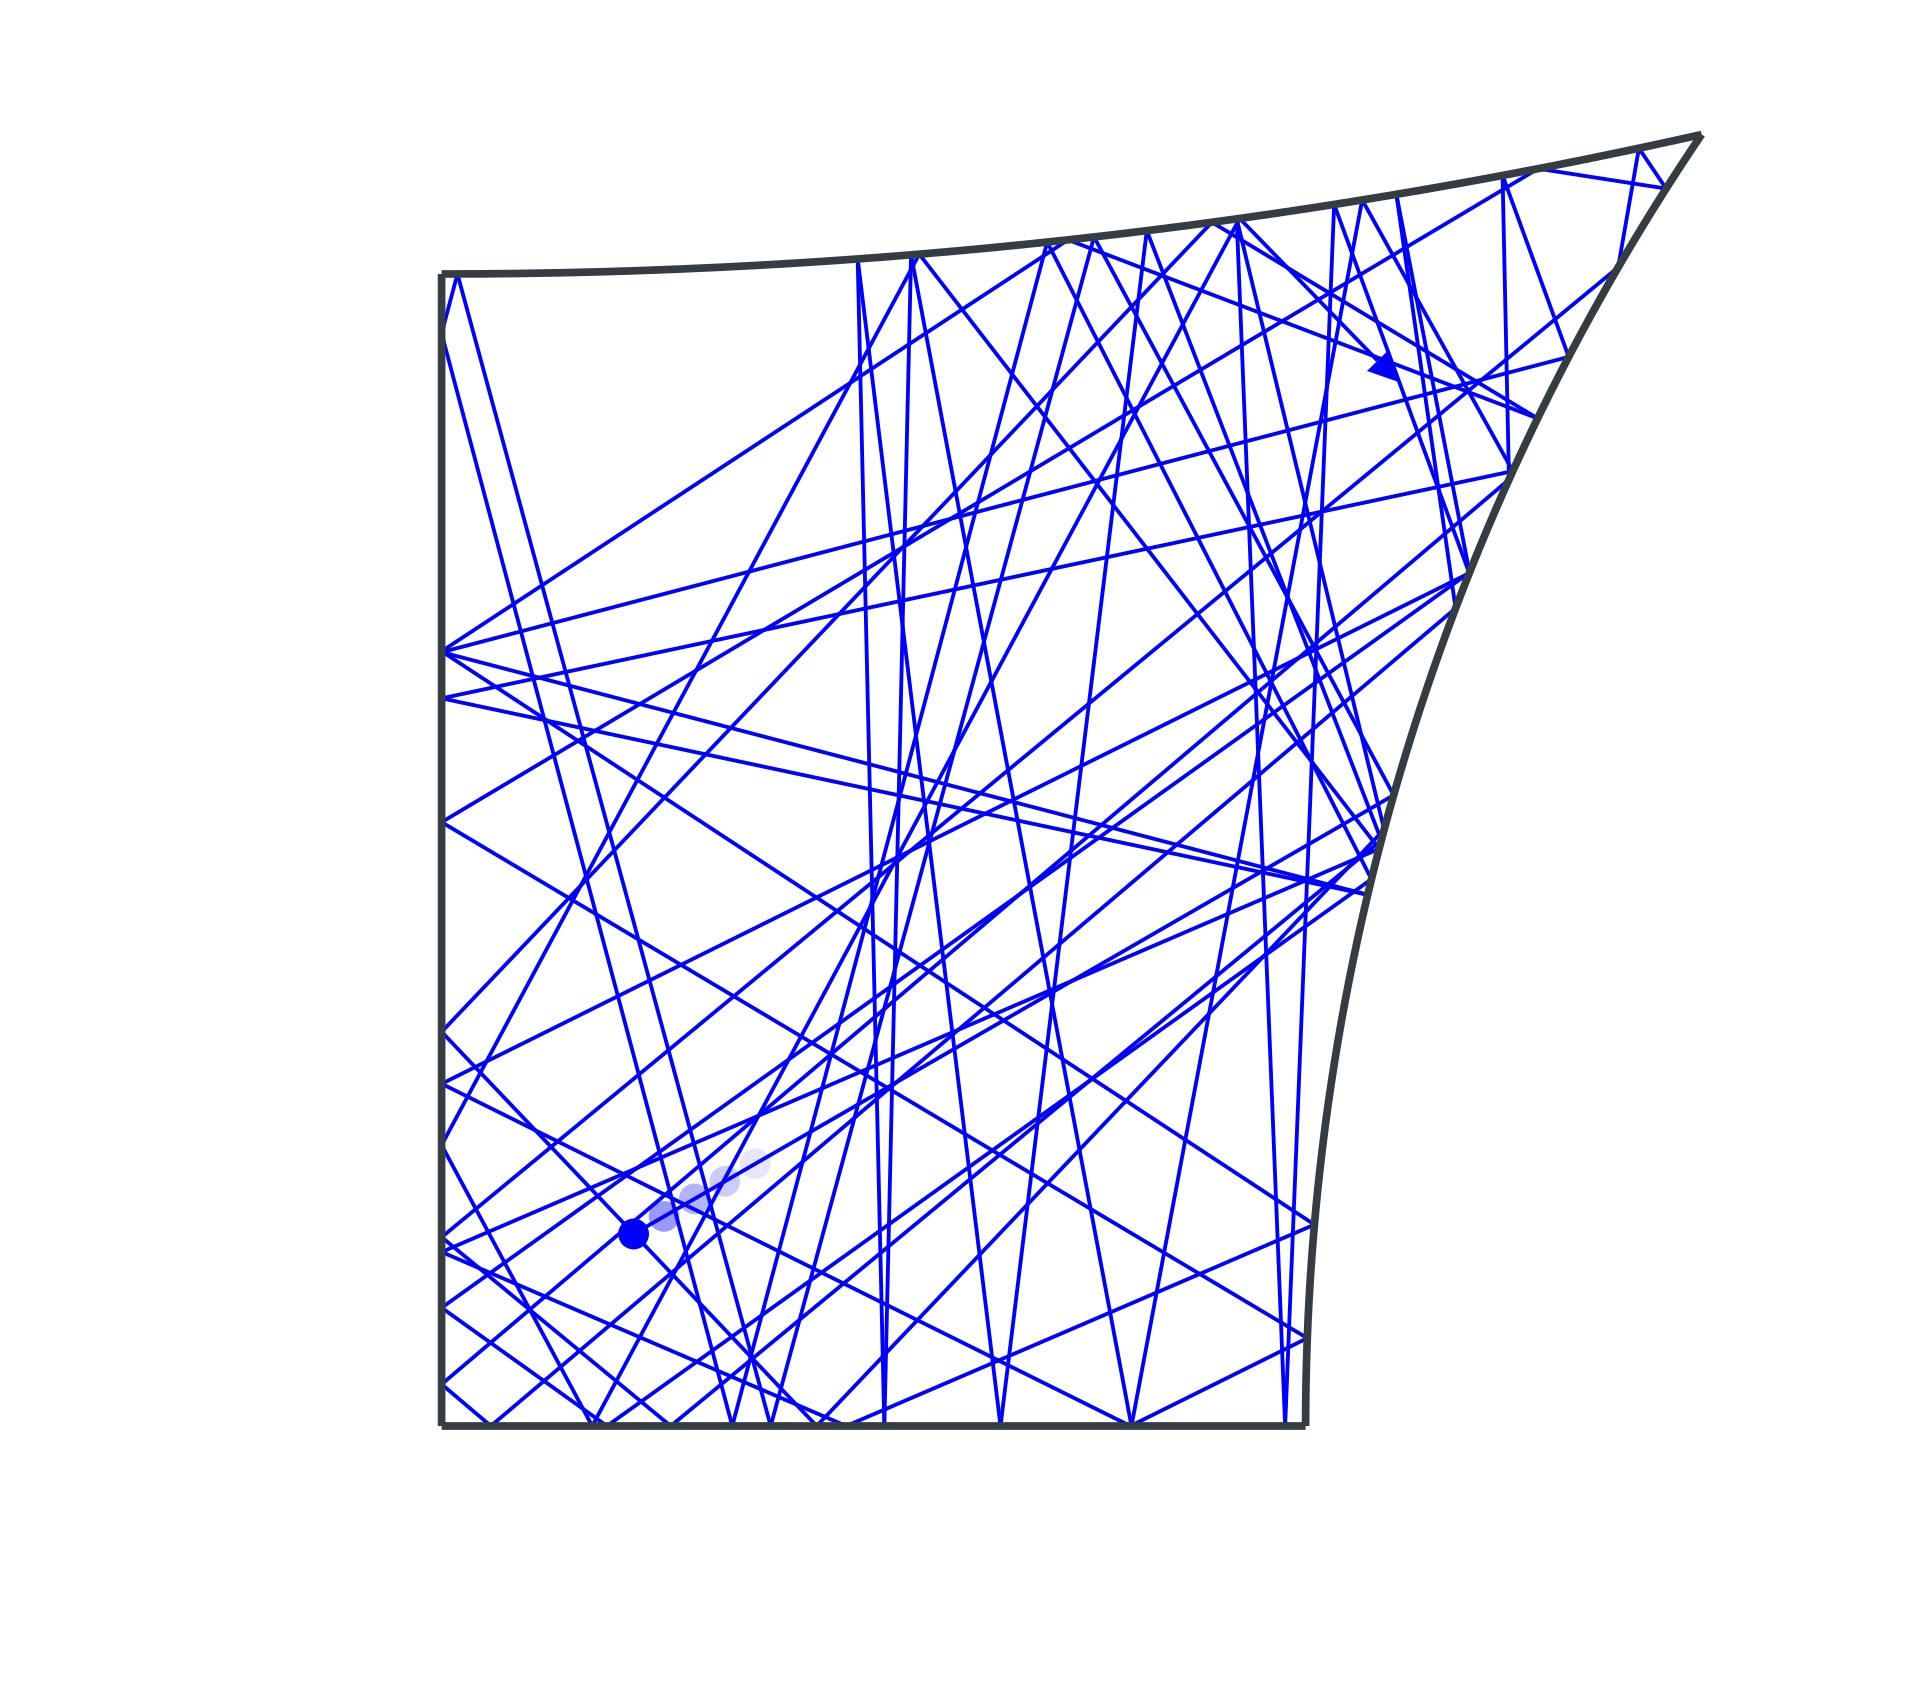
\includegraphics[scale=0.08,angle=0]{Barnett2.jpg}
    %\caption{Variabili $X_{n}$}
    \label{fig:barn1}
  \end{subfigure}
  %
  \noindent\\
  \decoRule
  \caption{Barnett's billiard.}
  \label{fig:barn_orbits}
\end{figure}

\begin{nese}[Cassini's billiard and cardioid billiard]
Other interesting billiards, which numerically share lots of properties of Bunimovich and Barnett billiards are the Cardioid billiard $\CS_{r}$, with domain defined by the cardioid of (polar) equation
\[
\rho(\theta)=r(1-\cos\theta)
\]
and the Cassini's oval billiard $\COS_{a,b}$ defined by the equation
\[
(x^{2}+y^{2})^{2}-2\cdot a^{2}(x^{2}-y^{2})+a^{4}=b^{4}, \quad a,b>0,\, b>a.
\]
In particular, for $b/a\geq\sqrt{2}$ is convex, otherwise for $1<b/a<\sqrt{2}$ it is peanut-shaped.
\end{nese}

\begin{figure}[H]
\centering
  %
  \begin{subfigure}[b]{0.5\textwidth}
  \centering
    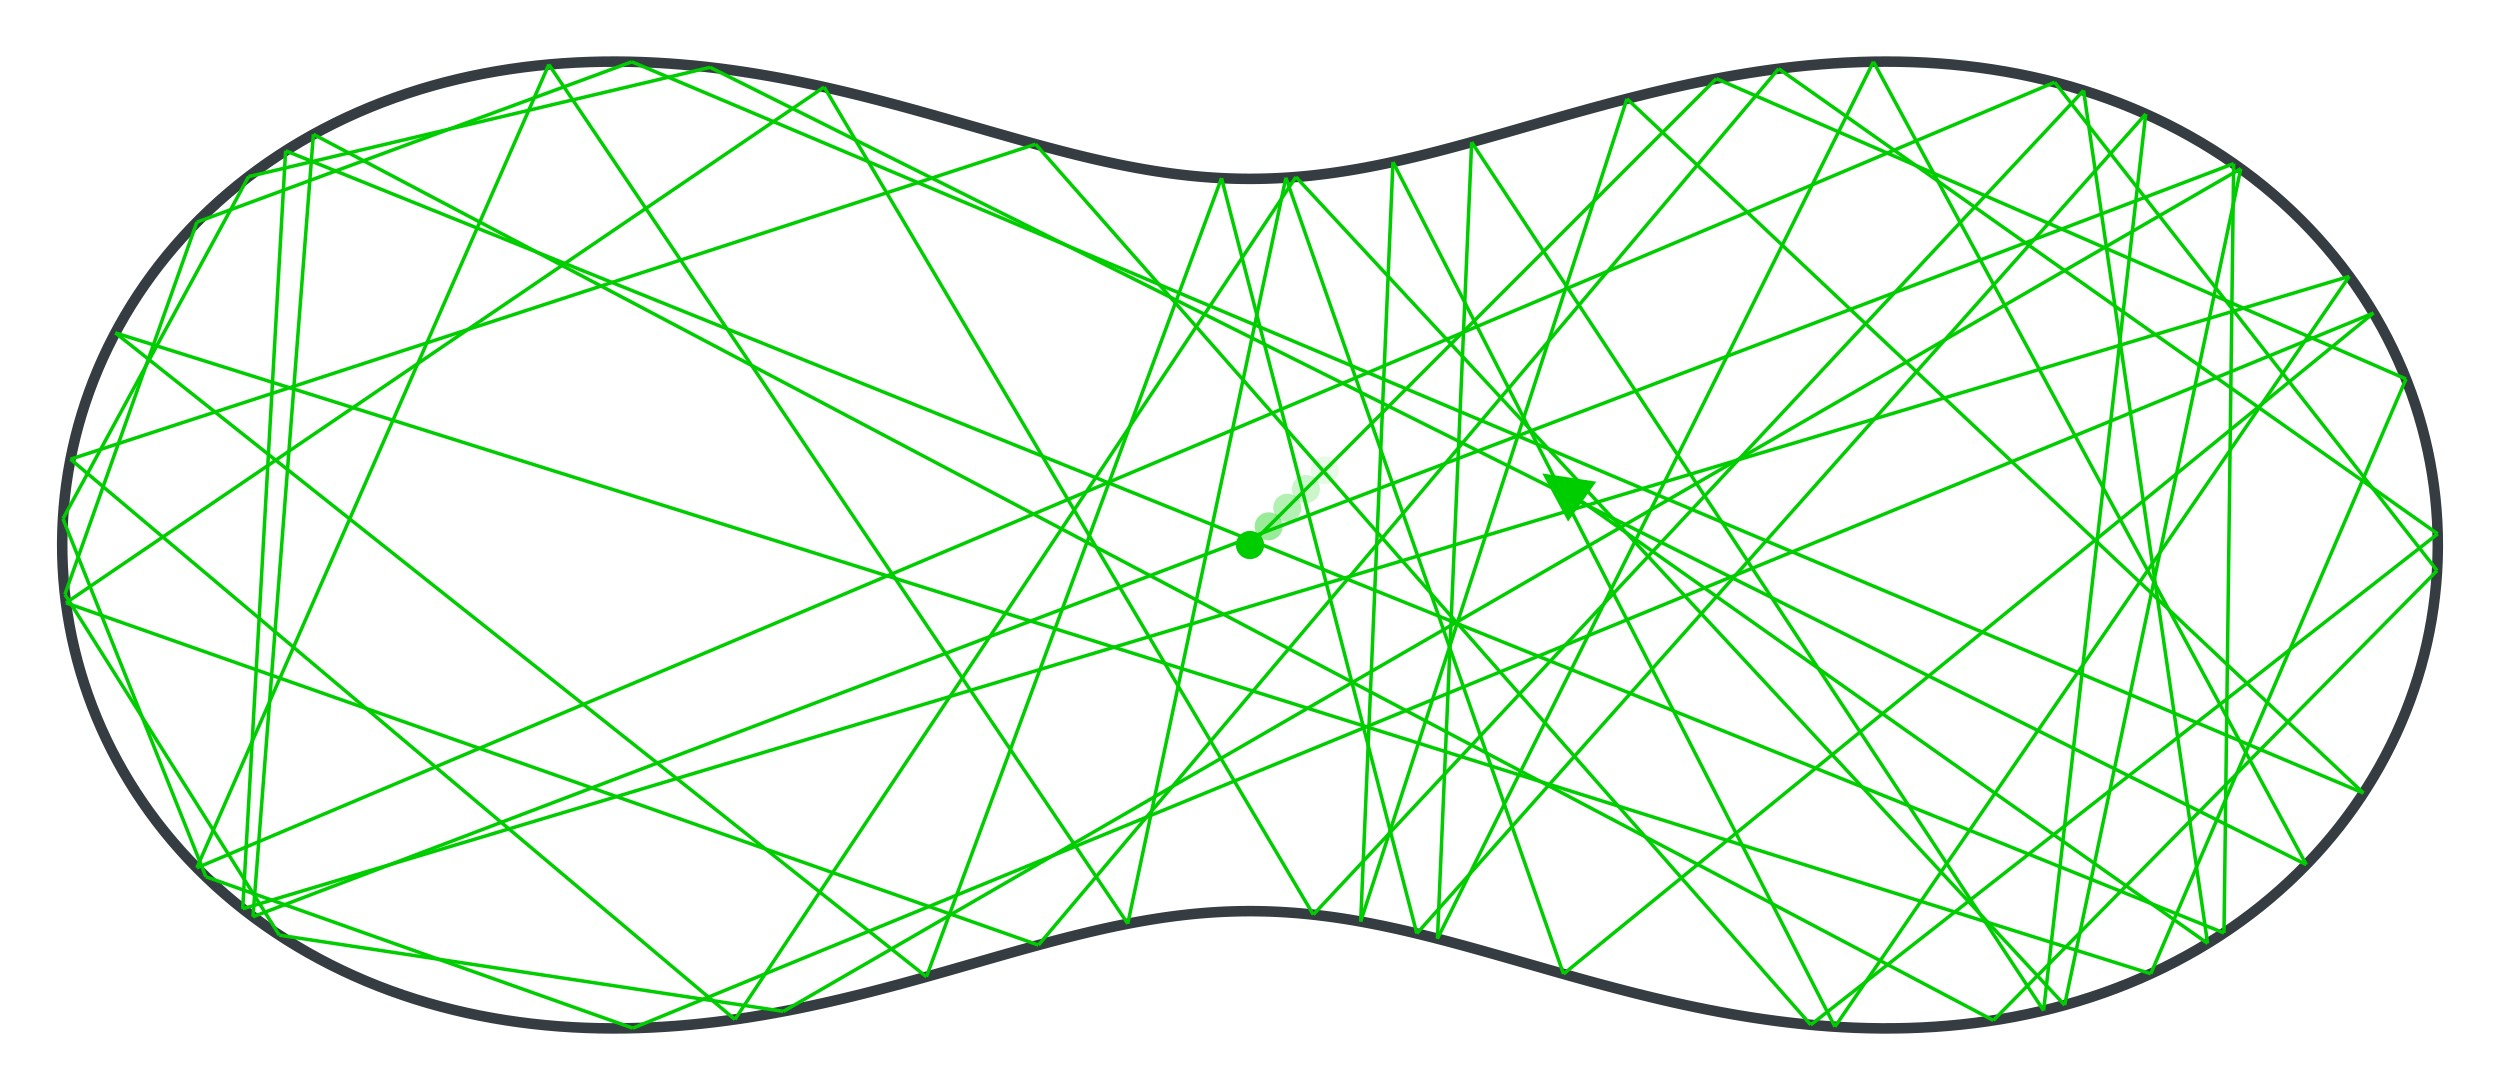
\includegraphics[scale=0.08,angle=0]{Cassini_true.jpeg}
    %\caption{Variabili $X_{n}$}
    \label{fig:oval}
  \end{subfigure}
    \noindent\\
  \begin{subfigure}[b]{0.4\textwidth}
  \centering
    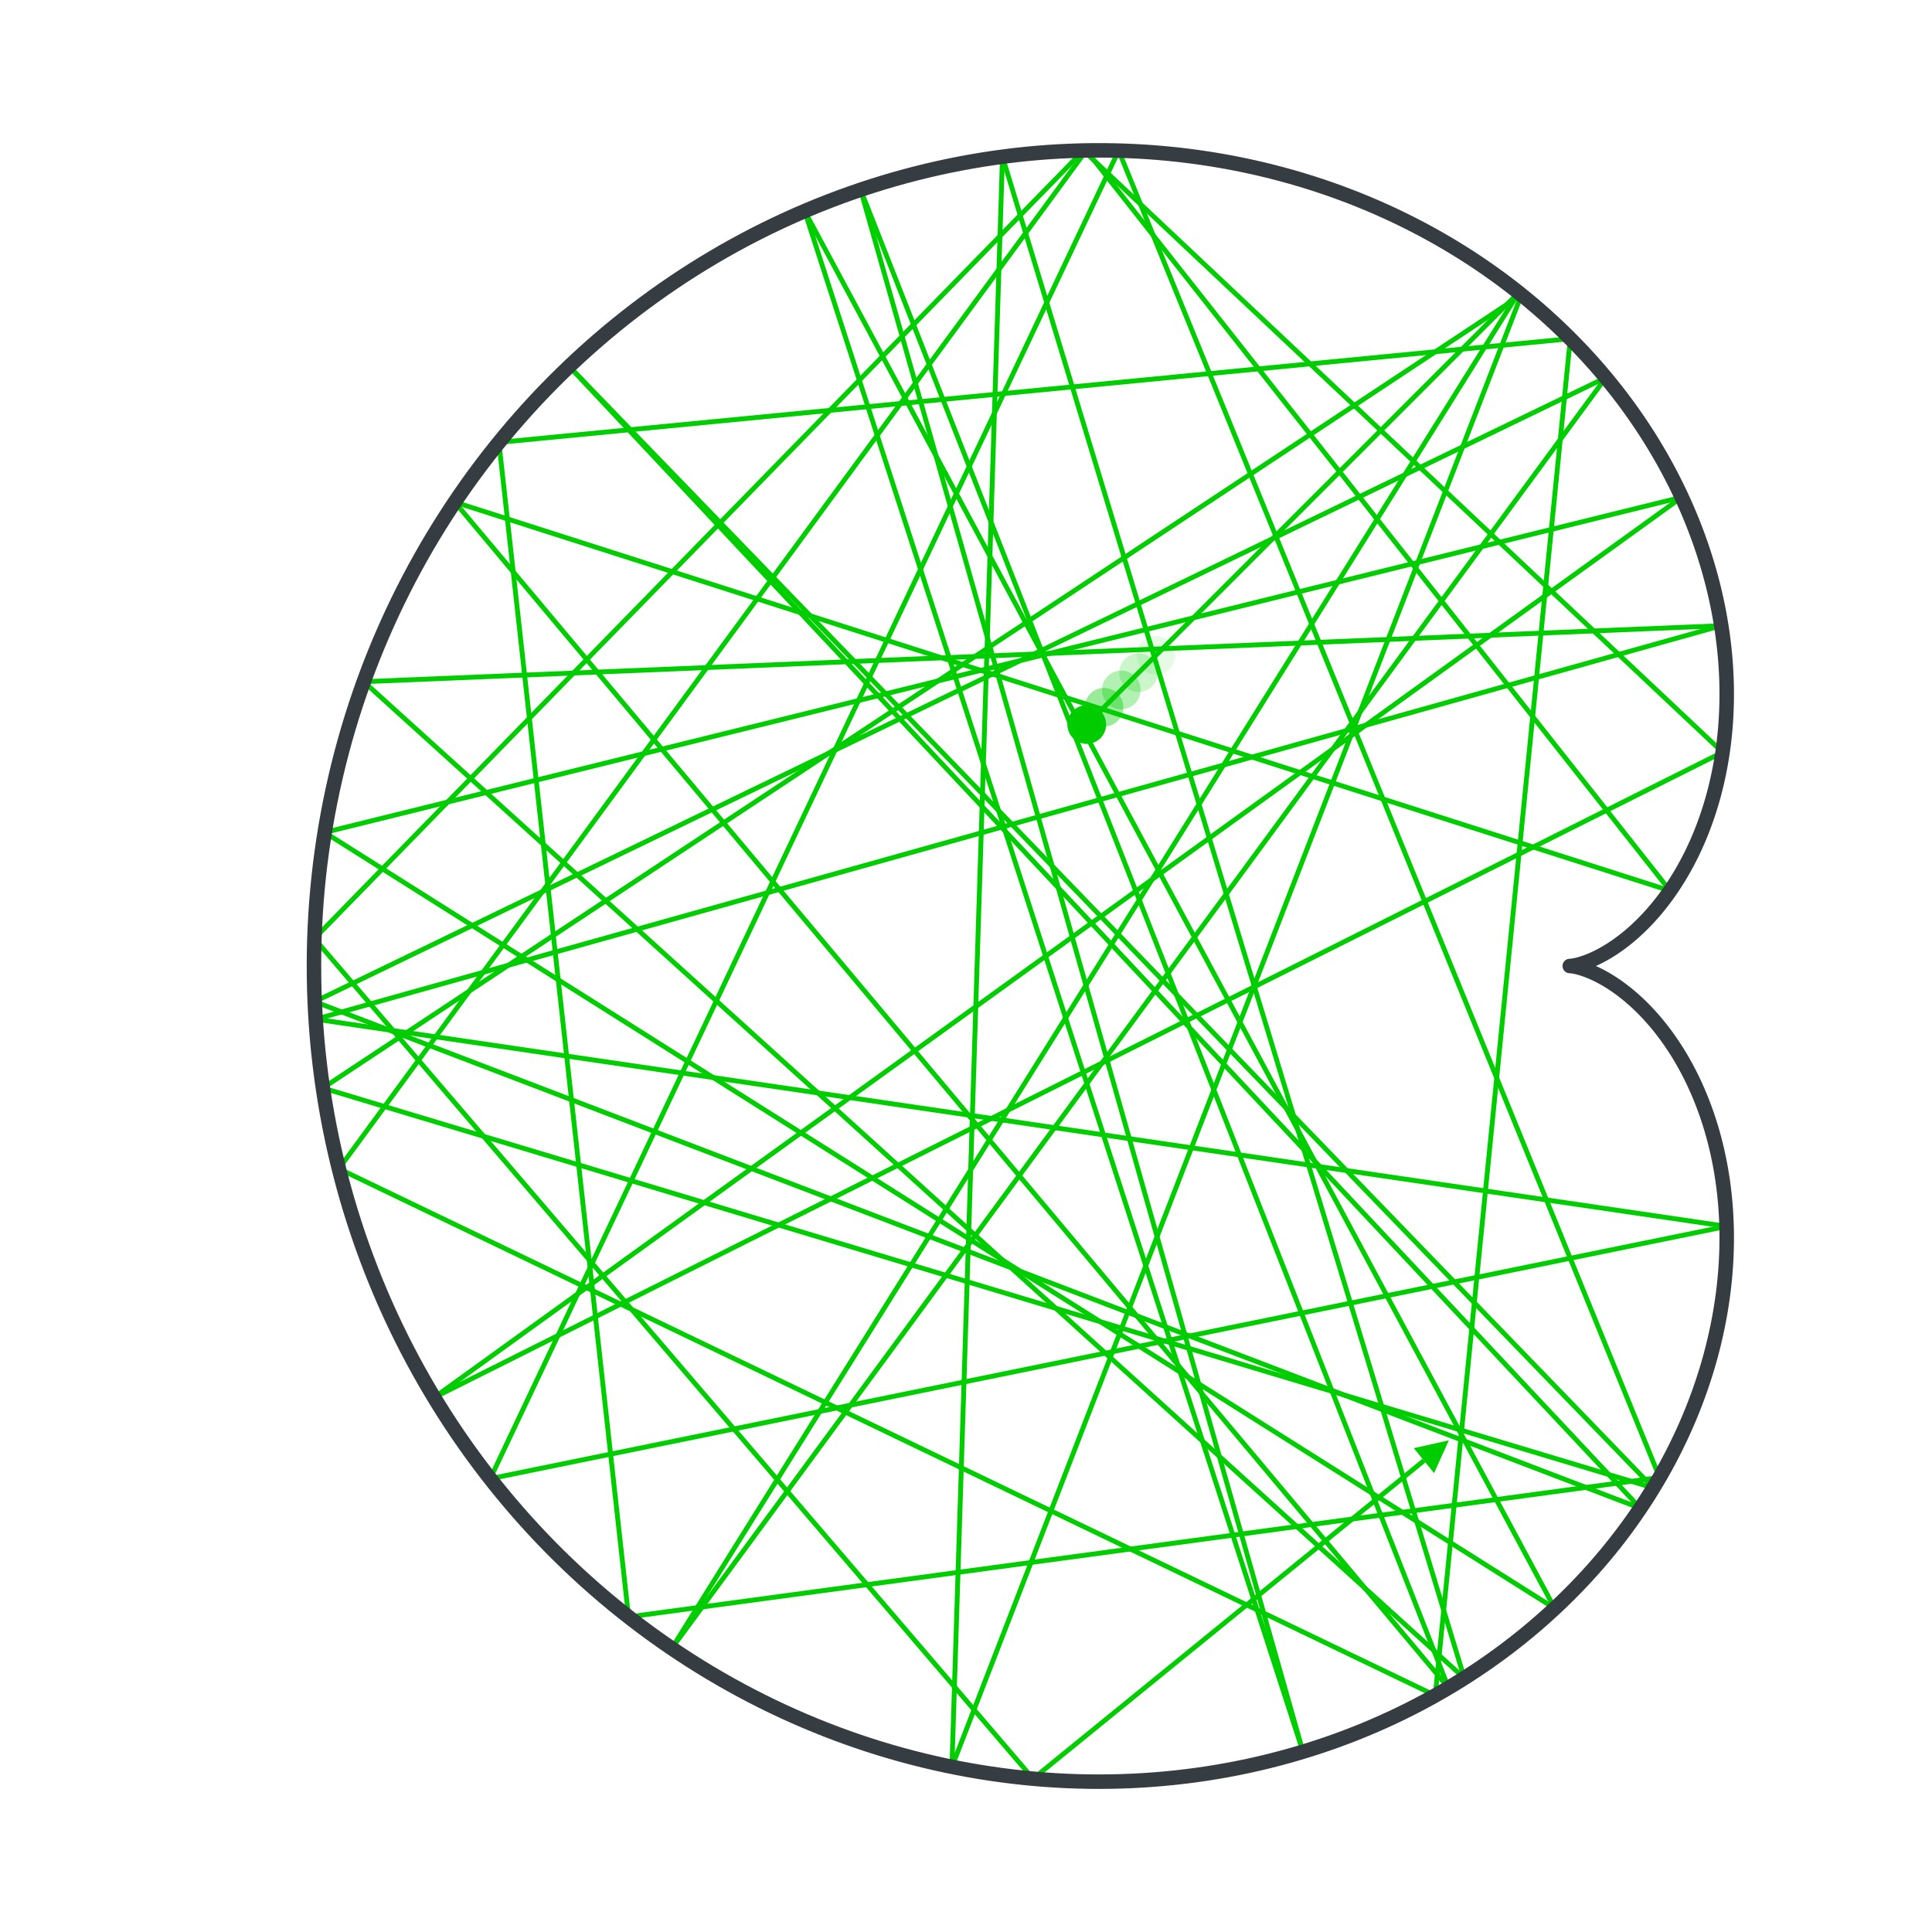
\includegraphics[scale=0.06,angle=0]{Cardioid.jpg}
    %\caption{Variabili $X_{n}$}
    \label{fig:cass}
  \end{subfigure}
  \noindent\\
  \decoRule
  \caption{Billiard trajectories in the Cassini's oval and Cardioid.}
  \label{fig:oval_card_orbits}
\end{figure}

As mentioned before, there are also \virg{billiards} induced by geodesic flow on a Riemannian manifold. The flow on the modular surface is a good example of this case (see chapter \ref{Chapter1}).

\begin{nese}[Modular surface]
It can be shown that on every Riemannian manifold with negative curvature, the geodesic flow $\Phi_{t}$ is ergodic (see Hopf theorem \ref{teo:Hopf_theorem}). The geodesic flow on the unit tangent space of the modular surface $\PSL_{2}\Z\setminus\Hilb$ (\ref{subsec:hyp_surfc}) is hence ergodic.
\end{nese}


\begin{figure}[H]
\centering
  %
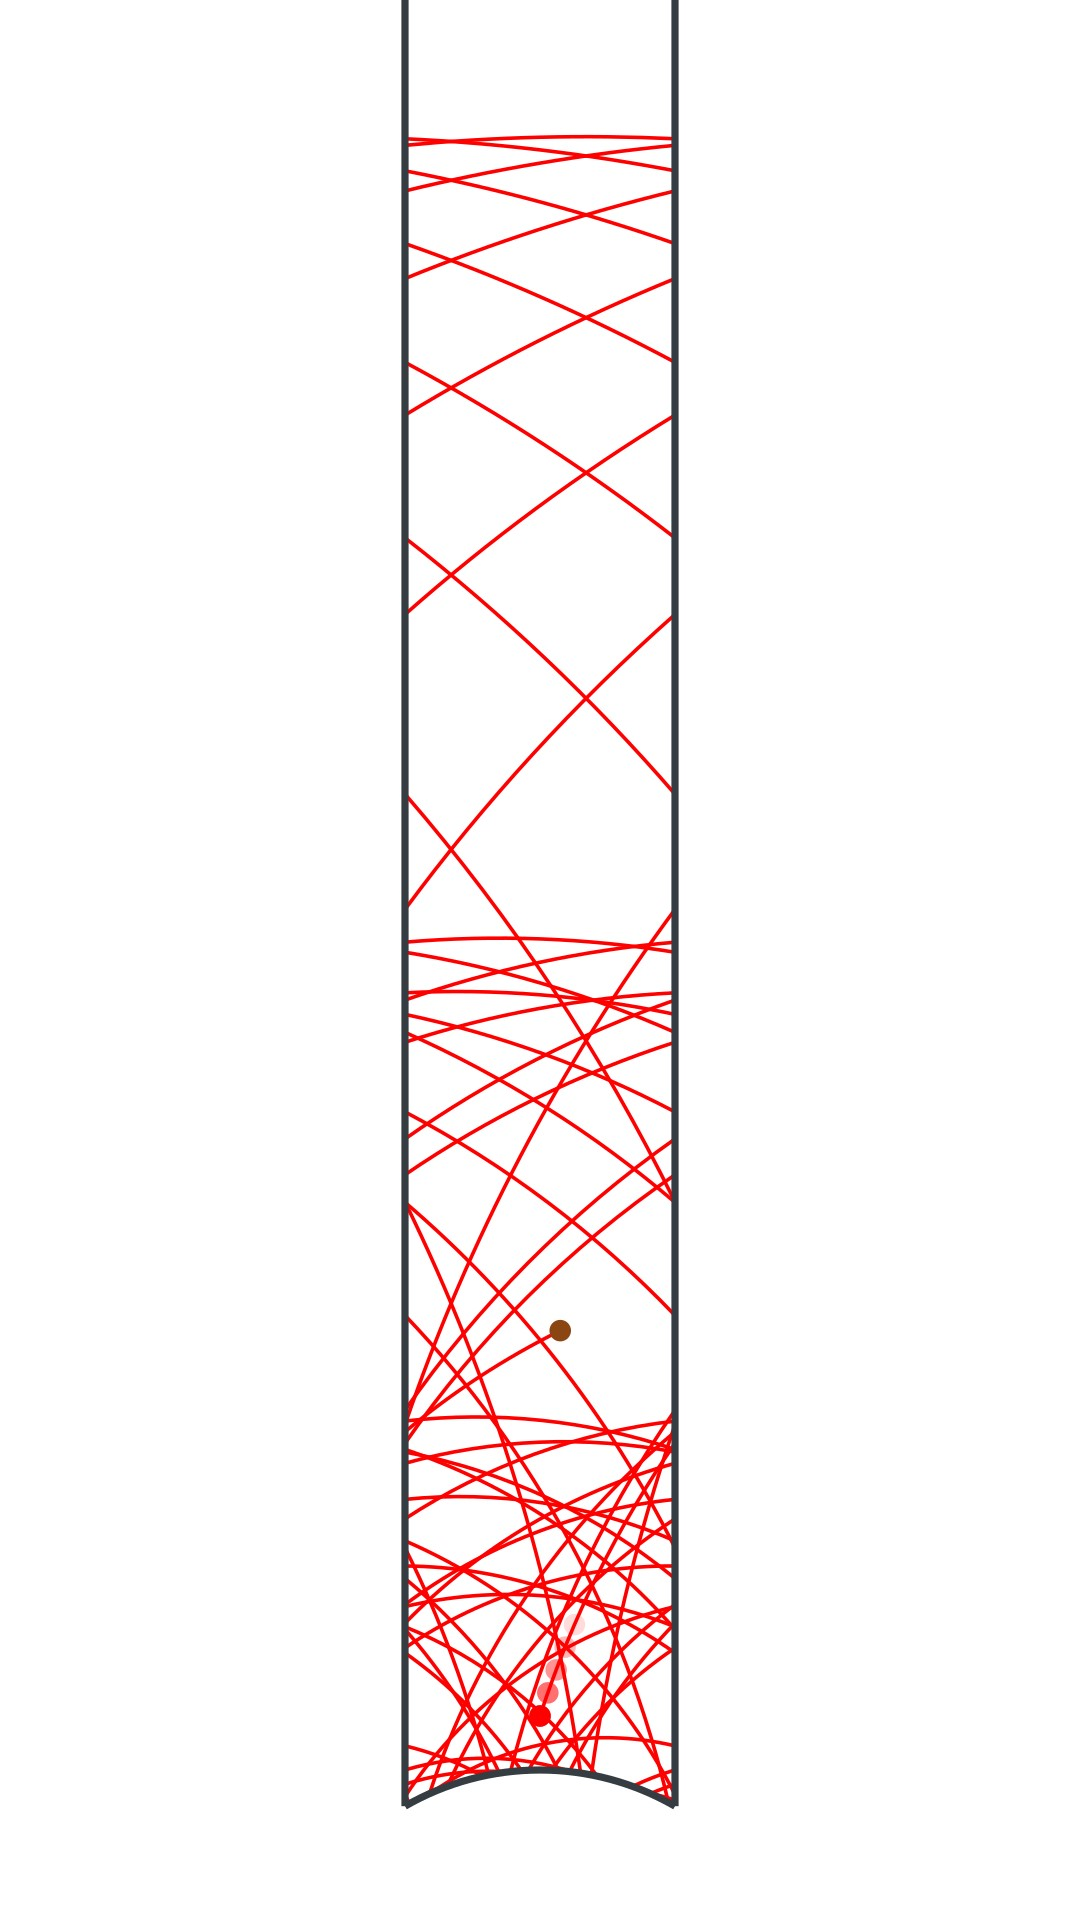
\includegraphics[scale=0.12,angle=0]{modular_good.jpg}
  \noindent\\
  \decoRule
  \caption{Ergodic orbit on the modular surface.}
  \label{fig:oval_card_orbits}
\end{figure}





\section{From classical to quantum billiards}


\subsection{Unique ergodicity}


Before introducing the \virg{quantum} definition of ergodicity, we recall the definition of unique ergodicity. In general, we give the following definition.

\begin{defin}
\label{def:unique_ergodic}
An ergodic metric system $(X,R,\mu_{L})$, where $\mu_{L}$ the standard Liouville measure, is called \emph{uniquely ergodic} if $\mu_{L}$ is the only finite borel measure, invariant with respect to $R$.
\end{defin}

The definition in the continuos case is essentially the same. The two condition of
\begin{compactenum}
\item finiteness,
\item uniqueness,
\end{compactenum}
are very strong. To this, consider a metric space $(X,R,\mu_{L})$, and a point $x\in X$ which is periodic. The dirac measure concentrated on points of the finite orbit of $x$ is preserved, but it is not the Liouville measure. We can appreciate the crucial point played by periodic orbits, in this framework.

\subsection{Quantum regime}

In quantum regime, billiards are described by wavefunctions $\psi_{n}$ whose time-evolution are ruled by the \emph{Schr{\"o}dinger equation}
\[
\imi\hbar\frac{\partial}{\partial t}\psi_{n}(x,t)=-\frac{\hbar^{2}}{2m}\Lapl\psi_{n}(x,t),
\]
where $\Lapl$ depends on the metric considered, with Dirichlet boundary conditions in the planar euclidian case. Moreover $\psi_{n}\in L^{2}(\Omega),\hbar$ is Planck's constant and $m$ is the mass of the particle. From quantum mechanics the generic time dependent solution is the superposition of time dependent solution of the form $\psi_{n}(x,t)=\exp(-\imi t E_{n}/\hbar)\vphi_{n}(x)$, where $E_{n}$ are quantum energy levels and $\vphi_{n}$ are eigenfunctions of the equation 
\[
-\frac{\hbar^{2}}{2m}\Lapl\vphi =E_{n}\vphi.
\]
So, the \virg{quantum-mechanical} evolution of the billiard is linked to the eigenvalue problem $-\Lapl\vphi_{n}=\lambda_{n}\vphi_{n}$, where $\lambda_{n}=2mE_{n}/\hbar^{2}$. Semiclassical analysis, among other things, deals with find a correspondence between classical motion and the quantum approach. Indeed, the starting question is: how is it possible to translate the concept of ergodicity in this quantum framework, from the classical one?

The feature of ergodicity that it is considered is equidistribution of orbits. We will know pause rigorous mathematical exposition for a brief informal introduction to the subject.\\
Let's consider the eigenfunction $\vphi_{j}$ corrispondent to the eigenvalue $\lambda_{j}$. Considering the absolute square $\abs{\vphi_{j}}^{2}$, we get a probability distribution on our billiard $\Omega$ or manifold $M$. There is a \emph{standard} way to lift this probability measure to the unit tangent space, using Wigner measures (see \ref{def:Wigner_measure} for further informations). Roughly speaking, for a smooth function $f\colon T^{1}\Omega=\Omega\times S^{1}$   on the unit tangent space, we can define the Wigner measure $\mu_{\vphi}$, and hence the integral $\mu_{\vphi}(f)$, induced by the eigenfunction $\vphi$ as 
\[
\mu_{\vphi}(f)\coloneqq\pscl{\Op(f)\vphi}{\vphi}_{L^{2}}
\]
where, if $\hat{\psi}$ is the Fourier transform of $\psi$,
\[
\Op(f)\psi(x)\coloneqq\int_{\R^{2}}\e^{2\pi\imi(x\cdot\xi)}\hat{\psi}(\xi)f\left(x,\frac{\xi}{\norm{\xi}}\right)\dd\xi.
\]
In particular, $\Op$ operator is a \emph{pseudo-differential operator} induced by function $f$. In \ref{subsec:how_to_quant} it is explained that this is only one possibilites, as there are other similar way to produce the operator $\Op$, e.g. another one is \emph{Weyl quantization}.\\
A \virg{natural way} to rewrite the idea \virg{a.e. orbit distributes itself uniformly} in the quantistic case is to formulate the following.

\begin{defin}
\label{def:roughly_qe_def}
A dynamical metric system is quantum ergodic if it does exist a subsequence of eigenvalues $\lambda_{k}$ for the Laplacian $\Lapl$ of density one, such that $\mu_{k}(=\mu_{\vphi_{\lambda_{k}}})$ converges weakly to the Liouville measure $\mu$.
\end{defin}

As will see in section \ref{sec:que_intro}, any weak limit for measures $\mu_{j}$ is called \emph{quantum limit}. Then, the concept of \emph{unique quantum ergodicity} is translated as follows.

\begin{defin}
\label{def:roughly_que_def}
A quantum system is unique ergodic if the only possible quantum limit is the standard Liouville measure.
\end{defin}

A case of particular interest is the one of hyperbolic surfaces $X$, with the Laplacian operator adapted to the hyperbolic metric \ref{sec:hyp_plane}. In this case, the Liouville measure is given by $\mu=\frac{1}{2\pi\lambda(X)}$, where $\lambda(X)$ is the hyperbolic measure of the hyperbolic surface $X$. The reason behind this interest is the following.

\begin{nteo}[Hopf]
\label{teo:Hopf_theorem}
Let $X$ be an hyperbolic surface. Then the geodesic flow on $T^{1}X$ is ergodic.
\end{nteo} 


\subsection{Some insights about \QUE}


A main result regarding \QE theory is due to Schnirelman,
Zelditch and Colin de Verdière, as we will see in chapter \ref{Chapter3}. Its statement is roughly the following.

\begin{nteo}
\label{teo:preview_quantum_ergod_theorem}
If a classical system is ergodic, then the corrisponding quantum system is \QE.
\end{nteo}

In particular, this gives us that Bunimovich stadium billiard $\BS$ and Barnett's billiard $\BarS$ are \QE. Moreover, all for all hyperbolic surface, \QE holds. So, the following question, made by Colin de Verdiére, was:
\begin{center}
What are the possible quantum limits?
\end{center}
Driven by theoretical considerations and numerical simulations, Rudnick and Sarnak proposed, in 1993 \cite{RudSarn:conj}, the following conjecture.\\[2mm]
\noindent\boldsf{Conjecture}: \emph{For all hyperbolic surfaces, \QUE holds}.\\[2mm]
A great achievement, towards this problem, was reached in 2010, thanks to the groundbreaking result due to Lindenstrauss. His work (\cite{LindBourg:entropy},\cite{Linden:main_art}) earned him the Fields Medal.

\begin{teo}[Lindenstrauss 2006, Soundarajan 2010]
\QUE holds for every arithmetic hyperbolic surface. 
\end{teo} 

Without goind in details about what an arithmetic hyperbolic surface is, it is sufficient to know that these surfaces arise from arithmetic methods. So, Lindenstrauss used this information to impose more symmetry on Laplacian eigenfunctions, via \emph{Hecke operators}, which are genuinely arithmetic tools.\\
On the other hand, another important result about \QUE led to the opposite side of the conjecture, in the euclidian case. In fact, in the same year (2010) Hassell proved that \QUE doesn't hold for Bunimovich stadium (\cite{Hass:billiards_not}), as some \virg{bouncing back and forth} eigenstates are still present in the high-energy limit. For more details, see chapter \ref{Chapter3}.


\section{The classic-quantum correspondence}

We have outlined the main themes of this thesis, so maybe it is a good time to recall what our aim is.\\
We are interested in understanding how the ergodicityof the geodesic flow does determin the distribution of high-eigenvalue Laplacian eigenfunctions. We recall some informations from appendix \ref{AppendixA}.\\

On any classical system on a Riemannian manifold $(M,g)$, the geodesic flow is given by the Hamiltonian vector field $X_{H}$ generated by the Hamiltonian function $H\colon M\to\R$. Integrating the Hamiltonian vector field $X_{H}$ generates a one parameter family of integral curves. These curves represent the geodesic flow and so we can define $\Phi^{t}\colon M\to M$ which defines the time evolution of a point on the manifold $M$ along this flow. In this context, the manifold $M$ is the configuration space, while the cotangent bundle $T^{\ast}M$ of couples $(q,p)$ of position and momentum is the phase space.\\
We can consider the energy level sets $\Sigma_{c}\coloneqq H^{-1}(c)$, which carry a natural flow-invariant measure, called \emph{Liouville measure}. It can be charaterized not only by the invariance through the geodesic flow, but also in the following way.

\begin{defin}
\label{def:Liouville_measure}
The Liouville measure $\mu_{L}^{c}$ is the flow-invariant volume-form on any \virg{energy-shell} $\Sigma_{c}$ of a Hamiltonian system. In particular, for $c\in [a,b]$, $\mu_{L}^{c}$ is characterized by the formula
\[
\iint_{H^{-1}[a,b]}f\dd x\dd p=\int_{a}^{b}\int_{\Sigma_{c}}f \dd\mu_{L}^{c}\dd c,
\]
for a smooth function $f\colon T^{\ast}M\to\R$.
\end{defin}

Now, if $(M,g)$ is a compact manifold with negative curvature, Hopf theorem \ref{teo:Hopf_theorem} assure us that the geodesic flow is ergodic, with respect to Liouville measure. In particular, we will show this in section \ref{sec:hyp_dynam}, in the case of hyperbolic surfaces generated by Fuchsian groups. The corrisponding quantum dynamics is the unitary flow generated by Laplace operator, as a generic time evolution is given by superposition of eigenfunctions $-\Lapl\psi=\lambda_{n}\psi$. At this level, we can \virg{see} that, in some way, the ergodic geodesic flow influences the spectral aspect of the Laplacian, making its eigenfunctions equidistributed.\\

Having this in mind, in our humble opinion, it seems appropriate to pointing out some important themes for this thesis. These will be useful to keep in mind in chapter \ref{Chapter3}.

\begin{compactitem}
\item Intuition behind the semiclassical limit: even if, numerically, we can take the \emph{semiclassical limit} $\hbar\to0$, we need the energies to be bounded. So, in semiclassical regime, we aspect that the asymptotic behaviour of quantum objects corrispond to the classical one; 
\item The technical aspects of semiclassical analysis: Fourier transform enables us to relate position and momentum variables. So, as semiclassical limit relies on a global rescaling, we will a sort of semiclassical Fourier transform, hence classical Fourier transform theory will be useful.
\item Interaction between order and disorder, from simple cases: as it can be seen, lots of the results and problem of this theory is drawn by visualization and numerical simulations; even if starting examples are very simple, the theory behind it isn't and this framework is a good example of the dichotomy between classical structure and quantum randomness:\\[2mm]
\textit{The \virg{dichotomy between structure(order) and randomness} seems to apply in circumstances
in which one is considering a high-dimensional class of objects$\ldots$ one needs tools such as algebra and geometry to understand the structured component, one needs tools
such as analysis and probability to understand the pseudorandom component, and one needs tools such as decompositions, algorithms, and evolution equations to separate the structure from the pseudorandomness.}\\[2mm]
\hspace*{10cm}\textsl{Terrence Tao}, \cite{tao:site_simons_lec}
\end{compactitem}


















% Chapter Template

\chapter{Hyperbolic geometry} % Main chapter title

\label{Chapter1} % Change X to a consecutive number; for referencing this chapter elsewhere, use \ref{ChapterX}
\thispagestyle{empty}
%----------------------------------------------------------------------------------------
%	SECTION 1
%----------------------------------------------------------------------------------------

\section{Iwasawa decomposition}

\begin{impTeo}{Iwasawa (real) decomposition}{iwasawa}
For every matrix $M\in\SL_{2}\R$ there exist real matrices $K,A,N$ such that $M=KAN$ and 
\begin{align*}
K\in\mathfrak{K}&=\SO_{2}\R\\
A\in\mathfrak{A}&=\left\{
\Smallmatrix{a&0\\0&a^{-1}}\,\colon a\in\R_{>0}
\right\}\\
N\in\mathfrak{N}&=\left\{
\Smallmatrix{1&b\\0&a1}\,\colon b\in\R
\right\}
\end{align*}
\end{impTeo}

The Iwasawa decomposition of a matrix $M$ ultimately let you see it's action as the composition of three fundamental subgroups of $\GL_{2}\R$. This decomposition naturally implies the same decomposition using the projective linear group $\PSL_{2}\R$ instead of $\SL_{2}\R$. This feature is of particular interest for us because, as we shall se, $\PSL_{2}\R$ is the isometry group of the hyperbolic plane.


\section{Hyperbolic models: upper-half plane and disk}

\label{sec:hyp_plane}
\subsection{Hyperbolic plane}

We will now introduce the hyperbolic plane and some of its fundamental charateristics. A good complete reference for hyperbolic geometry is \cite{Katok:groups}. As starting point, we will consider the \textbf{upper-half plane} model, i.e. the set 
\[
\Hilb = \R\times \R_{>0} = \left\{z\in\mathbb{C}\colon \Im(z)>0\right\}
\]
with the metric tensor given by 
\[
g=\frac{1}{y^{2}}(\dd x^{2}+\dd y^{2}).
\]
The couple $(\Hilb,g)$ gives us a Riemannian manifold, as the metric tensor $g$ is positive definined. Moreover we can compute the Gaussian curvature $\kappa$ of this model, using the fact that 
\[
\kappa=\frac{1}{2}\bar{R}
\]
where $\bar{R}$ is the Ricci scalar. The component of the Ricci tensor are obtained by contracting the indices of Riemann tensor $R\indices{_{abcd}}$ with the inverse metric tensor $g^{ac}$. Riemann tensor has $16$ components, but with easy calculations one ends up with 
\[
R\indices{^{1}_{212}}=-R\indices{^{1}_{221}}=R\indices{^{2}_{121}}=-R\indices{^{2}_{112}}=y^{-2}
\]
and all the other components vanish. Hence 
\[
R_{1212}=R_{2121}=-y^{-4}\text{ and }R_{1221}=R_{2112}=y^{-4}.
\]
It can be seen that, using Einstein notation, it holds
\[
R_{cadb}=y^{-4}(1-\delta_{ab}-\delta_{cd})(1-\delta_{ac}),\; g^{ab}=y^{2}\delta^{ab}
\]
Finally,
\begin{align*}
R_{ab} &= g^{cd}R_{cadb}=y^{2}\delta^{cd}y^{-4}(1-\delta_{ab}-\delta_{cd})(1-\delta_{ac})\\
& = y^{-2}(\delta^{cd}-\delta^{cd}\delta_{ab}-\delta^{cd}\delta_{cd}-\delta^{cd}\delta_{ac}+\delta^{cd}\delta_{ab}\delta_{ac}+\delta^{cd}\delta_{cd}\delta_{ac}) \\
& = y^{-2}(2-2\delta_{ab}-2-1+\delta_{ab}+1)=-y^{-2}\delta_{ab}
\end{align*}
and then
\[
R=g^{ab}R_{ab}=-2
\]
which yields $\kappa=-1$. This justify the \virg{hyperbolic} adjective, the upper-half plane model is an example of a manifold with constant negative curvature. As we shall se, this greatly modifies the geometrical properties that we are used to.

We will consider the tangent bundle $T\Hilb$ of the hyperbolic plane and the norm of a vector $\tau$ in the tangent space $T_{z}$ is given by
\[
\norm{\tau}_{z}=\sqrt{\pscl{\tau}{\tau}_{g,z}}=\frac{\abs{\tau}}{\Im(z)}.
\]
The unit tangent bundle is given by
\[
T^{1}\Hilb\coloneqq\left\{
(z,\tau)\in T\Hilb\colon \abs{\tau}=\Im(z)
\right\}
\]
of tangent vectors with lentgh 1. In this context, the (hyperbolic distance) between two points $z,w\in\Hilb$ can be defined as 
\[
d\colon\Hilb\times\Hilb\to[0,+\infty],\quad d(z,w)=\inf_{\gamma} L(\gamma)
\]
where the infimum runs over all curves $\gamma\colon[0,1]\to\Hilb$ such that $\gamma(0)=z,\gamma(1)=w$, and the length of the curve is defined as
\[
L(\gamma)\coloneqq\int_{0}^{1}\norm{\gamma'(t)}_{z}\dd t=\int_{0}^{1}\norm{\gamma'(t)}_{z}\frac{\dd t}{\Im(\gamma(t))}.
\]

It's interesting to determin and analyze the isometry group of $(\Hilb,g)$ with respect to the hyperbolic metric. More precisely, the set $\Isom(\Hilb)$ is the set of smooth maps $\vphi\colon\Hilb\to\Hilb$ that are metric-preserving, i.e. 
\[
\norm{\Diff\vphi(\tau)}_{\vphi(z)}=\norm{\tau}_{z},\quad\forall(z,\tau)\in TM
\]
The group $\PSL_{2}\R$ naturally acts on the extended hyperbolic plane $\hat{\Hilb}=\Hilb\cup\{\infty\}$ via \emph{M{\" o}bius transformations}. For any $A=\SmallQmatrix{a&b\\c&d}\in\PSL_{2}\R$, we get 
\[
A\ast z=\frac{az+b}{cz+d}
\]
if $z\in\Hilb$ and $A\ast\infty=a/c$, where $a/c=\infty$ if $c=0$. The action is well defined, as, if $\Im(z)>0$, than 
\[
\Im(A\ast z)=\frac{\Im(z)}{\abs{cz+d}^{2}}>0.
\]
For the sake of brevity, we will use $A(z)$ instead of $A\ast z$. This action generalize to an action on the unit tangent bundle $T^{1}M$ given by
\[
A\ast(z,\tau)=(A(z),\Diff A_{\ast}\tau).
\]
We will denote the action of $A$ on tangent vector $\tau$ at point $z$ with $\Diff_{z} A\tau$.\\

The action on $T^{1}M$ is faithfully and moreover is transitive. For this, it's sufficient to show that any element $(z,\tau)$ is in the $\PSL_{2}\R$-orbit of $(\imi,\imi)$. We have that
\[
\Qmatrix{1&x\\0&1}\Qmatrix{y^{1/2}&0\\0&y^{-1/2}}\imi=x+\imi y=z
\] 
and so, if $B=\SmallQmatrix{1&x\\0&1}\SmallQmatrix{y^{1/2}&0\\0&y^{-1/2}}=\SmallQmatrix{y^{1/2}&xy^{-1/2}\\0&y^{-1/2}}$, we have that $B^{-1}(z)=\imi$. In particular, the action of $B^{-1}$ on the tangent vector $\tau$ is the identity. Hence $B^{-1}\ast(z,\tau)=(\imi,\tau)$. Via straightforward computation, it can be shown that the subgroup $\SO_{2}\R$ is the stabilizer of point $\imi$ and acts as a rotation on the tangent vector $\tau$. In particular, if $\tau=e^{\imi\theta}$, let $\alpha=\frac{1}{2}\left(\frac{\pi}{2}-\theta\right)$. Then
\begin{align*}
\Diff_{\imi}\Qmatrix{\cos\alpha&-\sin\alpha\\ \sin\alpha&\cos\alpha}\imi&=\frac{\imi}{(\cos\alpha+\imi\sin\alpha)^{2}}=\imi \e^{-2\imi\alpha}\\
&=\imi \e^{-\imi\pi2}\e^{\imi\theta}=\imi(\imi)\tau=\tau
\end{align*}
and hence, if
\begin{equation}
\label{eq:main_matrix}
A=B\Qmatrix{\cos\alpha&-\sin\alpha\\\sin\alpha&\cos\alpha}=\Qmatrix{1&x\\0&1}\Qmatrix{y^{1/2}&0\\0&y^{-1/2}}\Qmatrix{\cos\alpha&-\sin\alpha\\\sin\alpha&\cos\alpha}
\end{equation}
we get that $A\ast(\imi,\imi)=(z,\tau)$. In particular this is the only matrix $A\in\PSL_{2}\R$ such that $A\ast(\imi,\imi)=(z,\tau)$. Hence, we have following.
\begin{nlem}
\label{lem:t1h_psl2_identification}
$T^{1}\Hilb$ and $\PSL_{2}\R$ are homeomorphic.
\end{nlem}
\begin{prf}
The action of matrix \eqref{eq:main_matrix} defines the desired homeomorphism.
\end{prf}

The group $\PSL_{2}\R$ coincides with the group $\Isom\Hilb$, as stated by the following theorem.

\begin{nteo}
\label{teo:area_volume_forms_invariants_isometries}
The left action of $\PSL_{2}\R$ on $T\Hilb$ it's transitive and preserves the area and volume forms
\[
\dd A=\frac{\dd x\wedge\dd y}{y^{2}},\quad\dd V=\frac{\dd x\wedge\dd y\wedge\dd\theta}{y^{2}}.
\]
In particular, the action of $A\in\PSL_{2}\R$ is an isometry.
\end{nteo}


At this point, it's crucial to establish some characterization of the geodesics, i.e. curves of minimal length connecting two given points. It can be shown the following result.

\begin{nprop}
\label{prop:geod_hyp}
The geodesics are the vertical lines and the semi-circles centred on the real axis.
\end{nprop}
\begin{prf}
Let $z,w\in\Hilb$. Let's assume first that $z=a\imi$ and $w=b\imi$, with $b>a>0$. Let $\eta(t)=t\imi$ with $t\in[a,b]$. Then 
\[
L(\eta)=\int_{a}^{b}\norm{\eta'(t)}_{\Hilb}\dd t=\int_{a}^{b}\frac{\abs{\imi}}{t}\dd t=\ln(b/a).
\]
Moreover, for a generic path 
\[
\gamma\colon[a,b]\to\Hilb,\,\gamma(t)=x(t)+y(t)\imi
\] 
such that $\gamma(a)=z$ and $\gamma(b)=w$, we have that
\[
L(\gamma)=\int_{a}^{b}\frac{\sqrt{x'(t)^{2}+y'(t)^{2}}}{y(t)}\geq\int_{a}^{b}\frac{\abs{y'(t)}}{y(t)}\dd t\geq\int_{a}^{b}\frac{\dd y}{y}=\ln(b/a)
\]
and hence $\ln(b/a)$ is the hyperbolic length of the segment of the $y$-axis joining $a\imi$ and $b\imi$. As this is valid for any point of the imaginary axis, we deduce that this axis is a geodesic.\\
Now, for two arbitrary points $z,w\in\Hilb$ it's sufficient to proceed as follows. Let $\mathcal{G}$ the unique vertical line or circle centered on the real axis passing through these two points. If $\mathcal{G}$ is a vertical axis $a+t\imi$, the matrix $\Qmatrix{1&-a\\0&1}$ shifts this line to the imaginary axis; if otherwise $\mathcal{G}$ is a semicircle with endpoints $a,b$ on the real axis, the matrix $\Qmatrix{0&-1\\1&-b}$ maps $\mathcal{G}$ to the imaginary axis. In both cases, with an element $A\in\PSL_{2}\R$ we can map $z,w$ on the imaginary axis and conclude as before. As $\PSL_{2}\R$ transformations are isometries, this shows what desired.
\end{prf}

Having described the hyperbolic geodesics, it would be useful to have a closed formula for the (hyperbolic) distance of two points. This is established by the following lemma.
\begin{nlem}
\label{lem:hyp_distance_formula}
For $z,w\in\Hilb$, we have 
\[
\cosh d_{\Hilb}(z,w)=1+\frac{\abs{z-w}^{2}}{2\Im(z)\Im(w)}.
\]
\end{nlem}
\begin{prf}
Let's assume first that $z=a\imi$ and $w=b\imi$, with $b>a>0$. Then 
\[
\cosh d_{\Hilb}(a\imi,b\imi)=\cosh\ln(b/a)=\frac{1}{2}\left(\frac{b}{a}+\frac{a}{b}\right)
\]
and 
\[
1+\frac{\abs{z-w}^{2}}{2\Im(z)\Im(w)}=\frac{a^{2}+b^{2}}{2ab}.
\]
Now, it's sufficient to show that the right hand side of the equality is invariant under the action of $A\in\PSL_{2}\R$ to conclude as in the previous result. This is left as exercise.
\end{prf}


Having the isometry group $\PSL_{2}\R$ of the upper-half plane model at hand and a characterization of geodesics, it's now possible to briefly describe the actions of an arbitrarly element $A\in\PSL_{2}\R$. In this regard, it's helpful to introduce another model of the hyperbolic plane, namely Poincaré's disk model $\Disk$, which is the data of $(\Disk,\Dmetr)$
\[
\Disk=\left\{
z\in\mathbb{C}\colon\,\abs{z}<1
\right\},\quad \Dmetr=\frac{4}{(1-\abs{z}^{2})^{2}}(\dd x^{2}+\dd y^{2})
\]
This model is totally equivalent with the upper-half plane model $\Hilb$ as they can be isometrically equivalent via the map 
\[
\Cayley\colon\Hilb\to\Disk,\quad\Cayley(z)\coloneqq\frac{\imi z+1}{z+\imi}
\]
induced, with abuse of notation, by the matrix $\Cayley=\frac{1}{\sqrt{2}}\SmallQmatrix{\imi&1\\1&\imi}$.\\

To see this, if $w=C(z)$ and $z=x+\imi y$ with $y>0$, then
\begin{align*}
\abs{w}^{2}&=\abs{\frac{\imi z+1}{z+\imi}}^{2}=\frac{\imi z+1}{z+\imi}\overline{\frac{\imi z+1}{z+\imi}}\\
&=\frac{x^{2}+y^{2}+1-2y}{x^{2}+y^{2}+1+2y}<1.
\end{align*}
Moreover, if $\tau_{1},\tau_{2}$ are tangent vectors at $z$, then corrispondent tangent vectors $v_{i}=\Diff\Cayley \tau_{i}$ at $w$ are given by
\[
v_{i}=\frac{\tau_{i}}{(z-\imi)^{2}}
\]
and with easy computation one can show that $\Hmetr(\tau_{1},\tau_{2})=\Dmetr(v_{1},v_{2})$.

This model can be more appropriate to describe some actions, as it's \virg{compact} and more symmetrical. In this model the geodesics are of two kind:
\begin{compactitem}
\item if $z,w\in\Disk$ are collinear with the origin $0$, then the geodesic is the only diameter passing through $z,w$;
\item otherwise, the geodesic connecting $z,w$ is the only circle passing through $z,w$ which is perpendicular\footnote{There is a nice geometrical construction for this: let $w^{\ast}$ be the point obtained inverting the point $w$ respect to the circle $\abs{z}=1$; the desired circle is the circle passing through $z,w,w^{\ast}$.} to $\partial\Disk$;
\end{compactitem}

\subsection{Hyperbolic isometries}

\label{subsec:hyp_isom}

As each element $A\in\PSL_{2}\R$ has determinat $1$, their action is determined by $\tr A$ (\textsc{wlog} we can assume $\tr A\geq0$, as $A$ is considered up to multiplication by $\pm I$). There are three cases:
\begin{compactitem}
\item $\tr A>2$, hyperbolic matrices;
\item $\tr A=2$, parabolic matrices;
\item $\tr A<2$, elliptic matrices.
\end{compactitem} 

Let's see briefly what their action is .\\[2mm]
\boldsf{Hyperbolic matrices}: $\tr A>2$\\
In this case, the eigenvalues are given by
\[
\lambda=\lambda_{1}=\frac{\tr A+\sqrt{\Delta}}{2}>1>\frac{\tr A-\sqrt{\Delta}}{2}=\lambda_{2}=\lambda^{-1},
\]
and are both real. If $v_{1},v_{2}$ are the two eigenvectors corrisponding respectivly to $\lambda_{1,2}$, matrix $A$ can be diagonalized by matrix $E=(v_{1}|v_{2})$, getting
\[
AE=E\Qmatrix{\lambda&\\&\lambda^{-1}}.
\]
Matrix $A$ acts on the plane $E\Hilb$ \virg{as} the matrix $D=\Smallmatrix{\lambda&\\&\lambda^{-1}}$ acts on $\Hilb$. In this case, the action is given explicity by $D(z)=\lambda^{2}z$ and this action is an (euclidian) homotety with center $0$ and factor $\lambda^{2}$. In particular, every points is attract to $\infty$ or to $0$ (depending whatever $\lambda\lessgtr1$).\\
For this reason, matrix $A$ it's a (hyperbolic) dilatation, of center $E\ast0$, factor $\lambda^{2}$ and direction $E\ast\infty$.%\\[2mm]

\begin{figure}[H]
\centering
  %
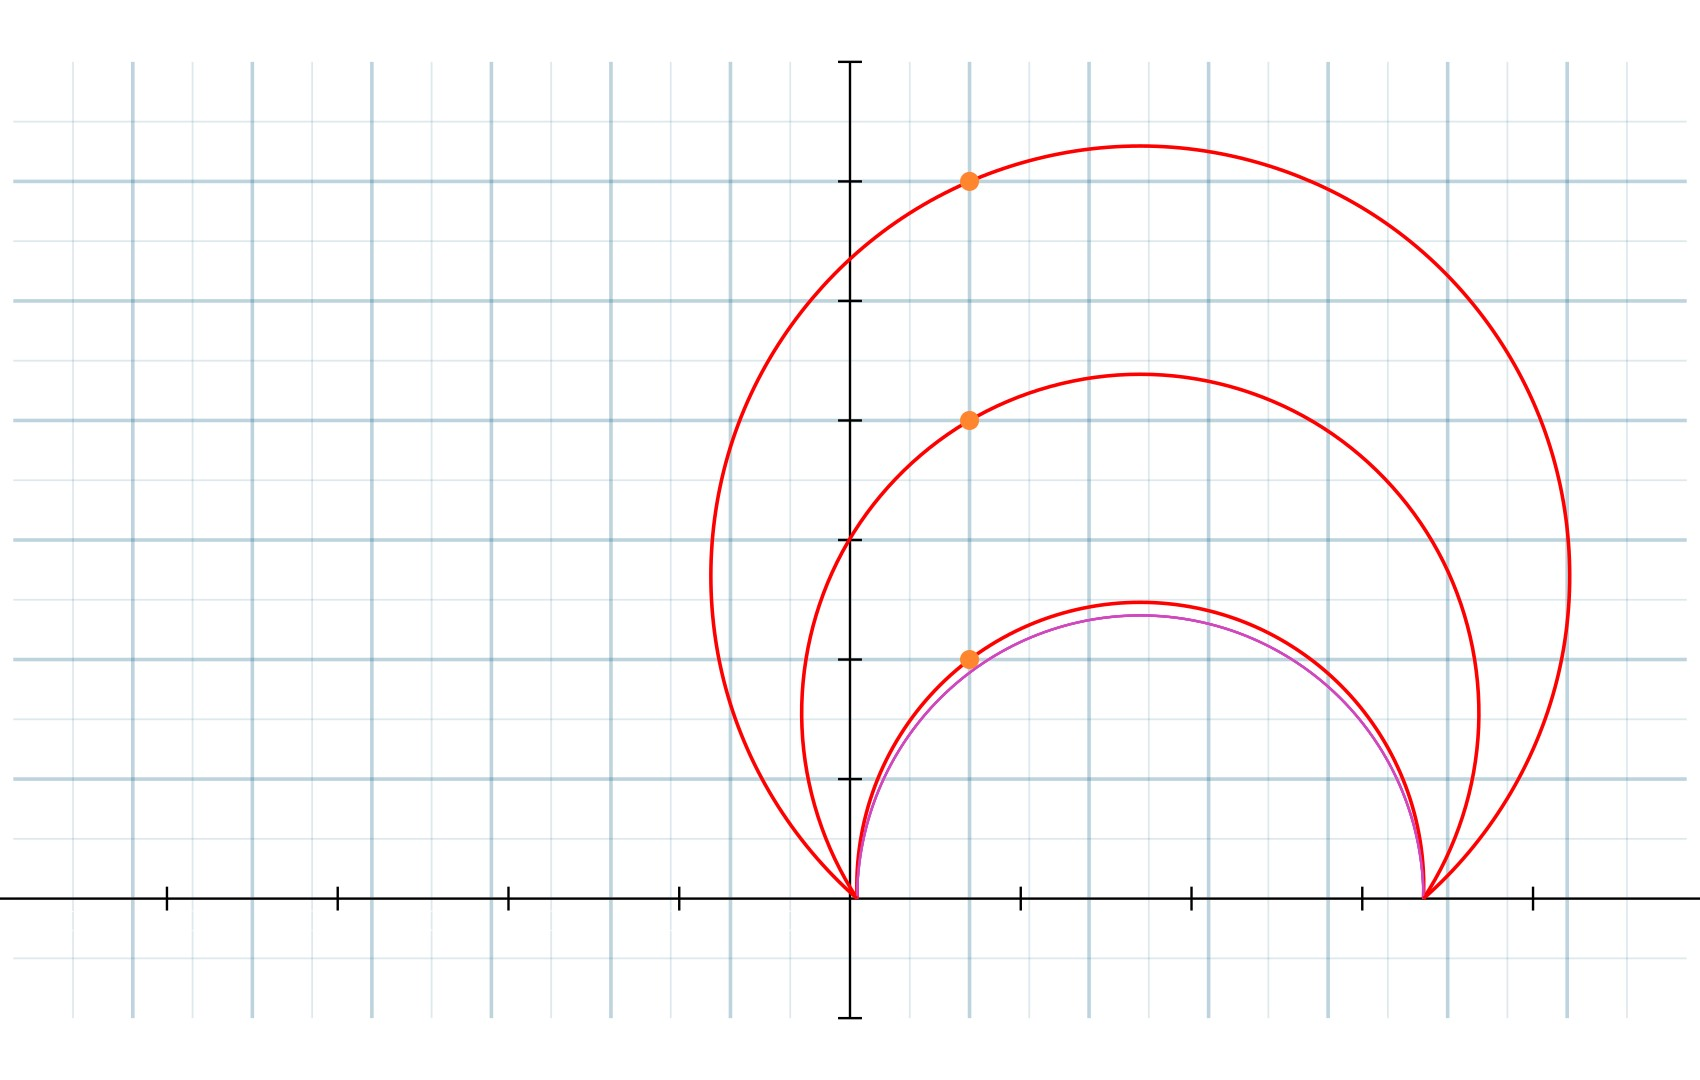
\includegraphics[scale=0.2,angle=0]{hyp_actions_hyp.jpg}
  \noindent\\
  \decoRule
  \caption{Action of an hyperbolic matrix on three point. In purple the \emph{axis}, see the end of this section.}
  \label{fig:hyp_action_hyp}
\end{figure}

\boldsf{Parabolic matrices}: $\tr A=2$\\
In this case the two eigenvalues are $\lambda_{1,2}=\lambda=1$. The matrix $A$ cannot be diagonalized, but it's similar to a matrix $D=\SmallQmatrix{1&T\\&1}$. In fact, fixed an eigenvector $v$ of $A$ for the eigenvalue $1$, this can form a basis for $\R^{2}$ with another indipendent vector $v'$. Moreover, re-scaling vector $v'$, we can suppose that $E=(v|v')$ has determinant $1$. Hence
\[
AE=E\Qmatrix{1&T\\&1}.
\]
As before, $A$ acts on the plane $E\Hilb$ \virg{as} the matrix $D=\Smallmatrix{\lambda&\\&\lambda^{-1}}$ acts on $\Hilb$. The action of $D$ is $D\ast z=z+T$, which is a horizontal translation with fixed point $\infty$. In particular, the orbits induced by $D$ can be considered as cirles of infinity ray with center at $\infty$. With this point of view, it's easy to describe the action of $A$: it's action will be a hyperbolic translation along circles which are tangets with line $\R\cup\{\infty\}$ at point $E\ast\infty$.%\\[2mm]
\begin{figure}[H]
\centering
  %
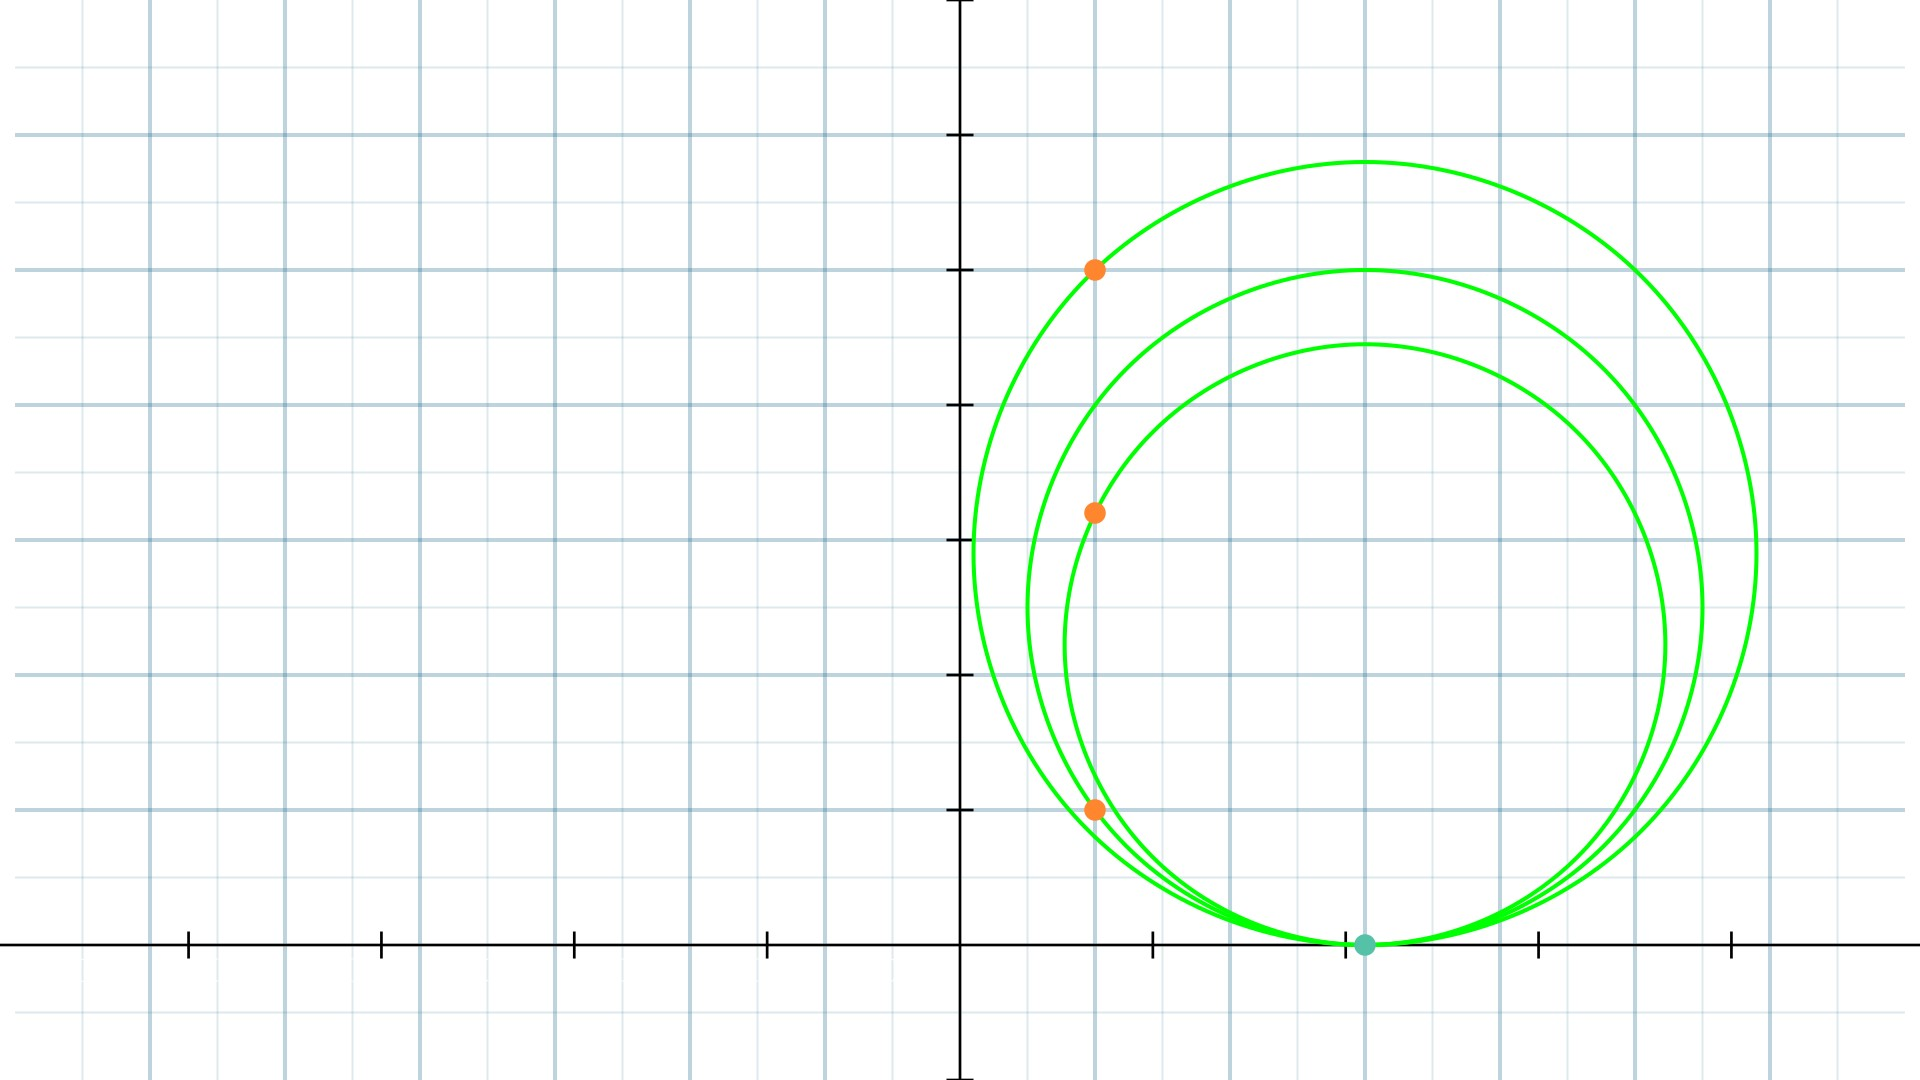
\includegraphics[scale=0.2,angle=0]{hyp_actions_parab.jpg}
  \noindent\\
  \decoRule
  \caption{Action of a parabolic matrix on three point.}
  \label{fig:hyp_action_parab}
\end{figure}


\boldsf{Elliptic matrices}: $0<\tr A<2$\\

In this case the eigenvalues are complex conjugated $\lambda=\lambda_{1}=\bar{\lambda}_{2}$ of modulus $1$ ($\lambda=e^{\imi\theta}$). Let $v$ the eigenvector corrisponding to the eigenvalue $\e^{\imi\theta}$, so that $\bar{v}$ is the eigenvector for $\e^{-\imi\theta}$. Let $E=(v+\bar{v},\imi(v-\bar{v}))$. Scaling $E$, we can make $\abs{\det T}=1$. 
\begin{figure}[H]
\centering
  %
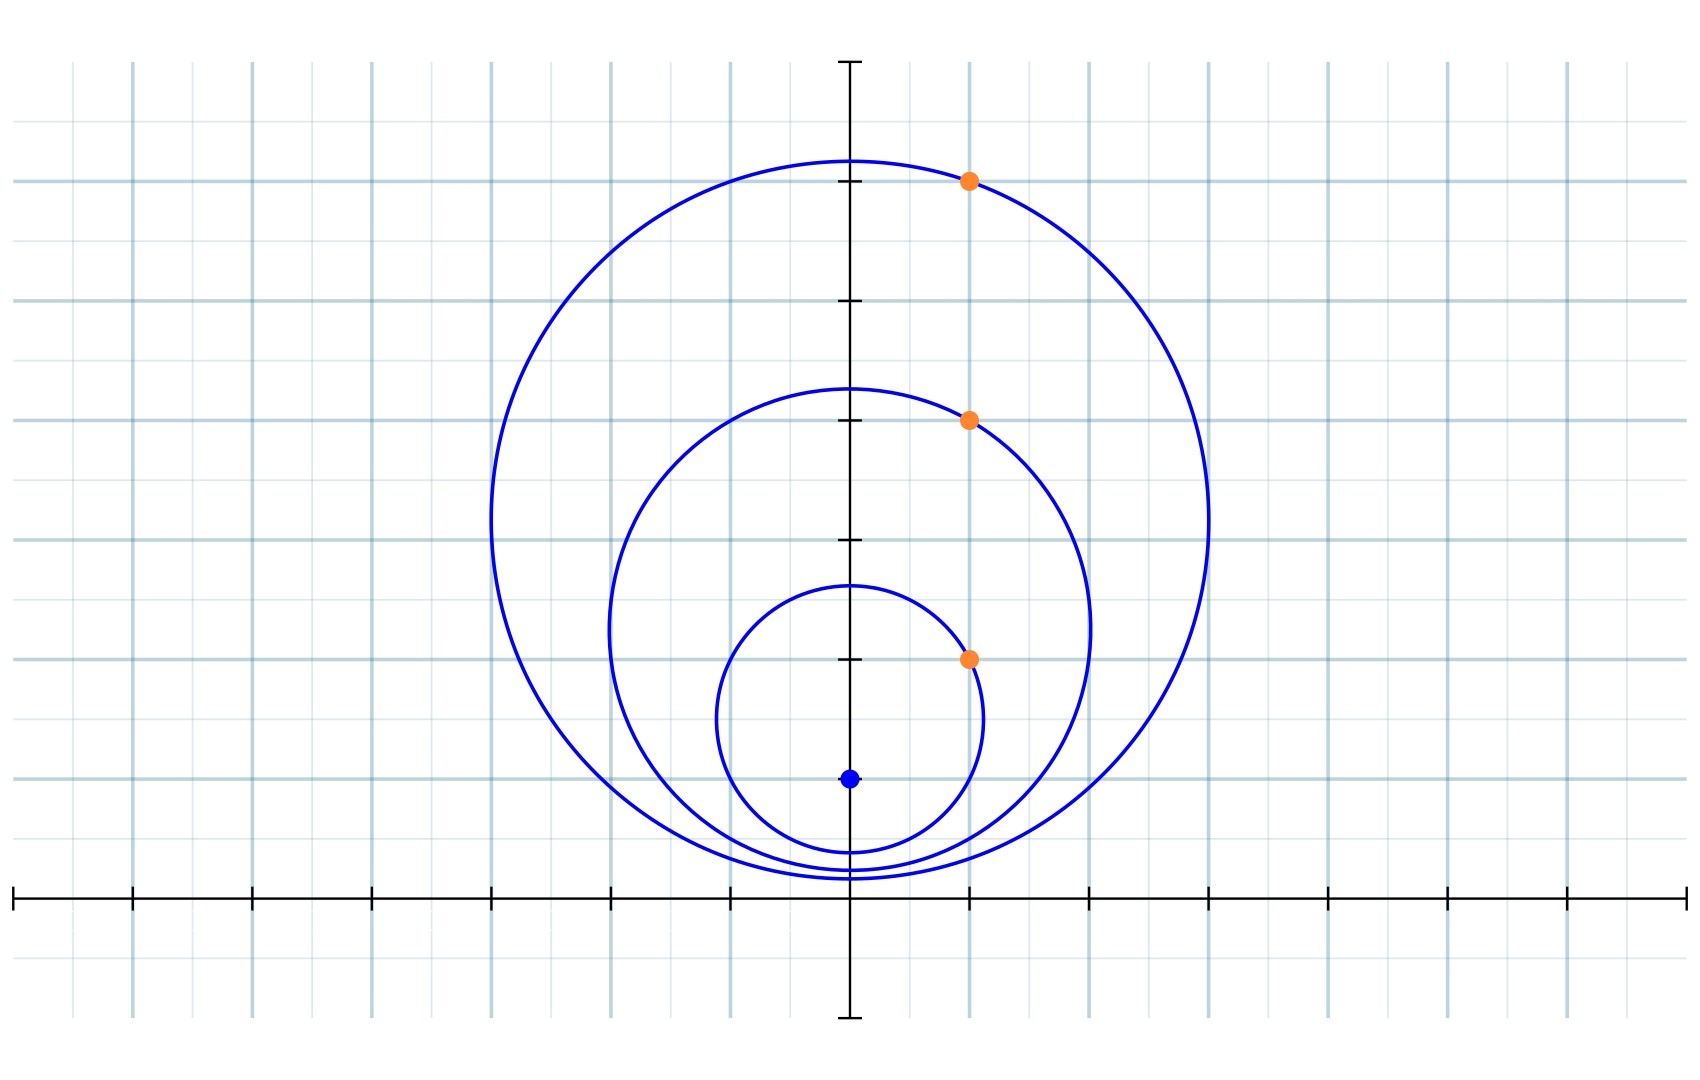
\includegraphics[scale=0.2,angle=0]{hyp_actions_ell.jpg}
  \noindent\\
  \decoRule
  \caption{Action of an elliptic matrix on three point.}
  \label{fig:hyp_action_ell}
\end{figure}
Let's assume $\det E=1$ (the other case is totally analogue). In this case,
\[
AE=E\Qmatrix{
\cos\theta&-\sin\theta\\\sin\theta&\cos\theta
}=ER
\]
$R$ fixes the point $\imi$. The action of $R$ can better visualized in Poincaré's disk model $\Disk$: the matrix $\Cayley$ sends $\imi$ in $0$ and the corrisponding matrix is given by
\[
\Cayley R\Cayley^{-1}=\Qmatrix{\e^{-\imi\theta}&\\&\e^{\imi\theta}}
\] 
and so the action on $\Disk$ is given by $z\mapsto\e^{-2\imi\theta}z$, which is exactly a rotation of angle $2\theta$ clockwise. In conclustion, the action of $A$ on $E\Hilb$ is given by hyperbolic rotations around the (unique) fixed point of $A$ in $\Hilb$.\\[2mm]

We could ask ourselves if any action of these matrices could send a geodesic into itself. In this sense, let's recall Iwasawa decomposition \ref{impTeo:iwasawa}: the action of a matrix is decomposed into the product $KAN$. Hence, given a matrix $KAN=M\in\PSL_{2}\R$, it's sufficient to check if there is an invariant geodesic whene $M$ is in one of three subgroups of Iwasawa decomposition.\\
If $M\in\PSO_{2}\R$, then $M$ it's a (hyperbolic) rotation around $\imi$ and then there is no invariant geodesic. In the same way, even if $M=\SmallQmatrix{1&x\\0&1}$ there are no invariant geodesics, as $M$ is an horizontal translation.\\
Diagonal matrices $A_{t}=\SmallQmatrix{\exp(t/2)&0\\0&\exp(-t/2)}$ instead send the $0-\infty$ geodesic into itself (and $0,\infty$ are fixed points for $A_{t}$). In general, an hyperbolic matrix $M$ with $\abs{\tr M}>2$ is conjugate to a matrix $A_{t}$ and so the geodesic connecting the two (real) fixed points of $M$ is invariant under the action of $M$.

It's possible to give an explicit description of this geodesic. Let $M=\SmallQmatrix{a&b\\c&d}$, then the fixed points are given by
\[
z_{1,2}=\frac{-(d-a\pm\sqrt{(d-a)^{2}+4cb})}{2c}=-\frac{d-a}{2c}\pm\frac{\sqrt{(d+a)^{2}-4}}{2c}
\]
and so the desired geodesic is the semicircle of center $z_{C}=-(d-a)/2c$ and radius $r=\sqrt{(d+a)^{2}-4}/(2\abs{c})$. So the equation of the geodesic is 
\begin{equation}
\label{eq:invar_geodes_hyperb}
\abs{z-z_{C}}^{2}=r^{2}\;\Leftrightarrow\;c\abs{z}^{2}-(d-a)\Re(z)-b=0
\end{equation}

If $c=0$, then the invariant geodesic is vertical, the details are left. In general, such an invariant geodesic is called \emph{\textbf{axis}} of hyperbolic matrix $M$.




\subsection{Hyperbolic surfaces and fuchsian groups}

\label{subsec:hyp_surfc}

The starting point to construct hyperbolic surfaces is to consider the analogue of euclidian lattice in this hyperbolic contest, i.e. fuchsian groups. The following result defines a fuchsian group.

\begin{nteo}
\label{teo:fuchs_theom_def}
Let $\Gamma$ be a $\PSL_{2}\R$ subgroup. The following are equivalent:
\begin{compactitem}
\item The action of $\Gamma$ on $\Hilb$ is properly discontinuos;
\item Each $\Gamma$-orbit on $\Hilb$ is discrete and each point has finite stabilizer;
\item $\Gamma$ is discrete with respect to $\PSL_{2}\R$ topology.
\end{compactitem}
\end{nteo}


\begin{defin}[Fuchsian group]
\label{def:fucs_def}
A subgroup $\Gamma$ of $\PSL_{2}\R=\Isom\Hilb$ that satisfies one of theorem \ref{teo:fuchs_theom_def} conditions is called \emph{fuchsian group}.
\end{defin}

We can get an \underline{hyperbolic surface} by considering the quotient $\Gamma\setminus\Hilb$. In this way, $M$ it's not necessarily a Riemann surface; in fact, if $\Gamma$ contains some elliptic points then $M$ it's an object called \emph{orbifold}. In general, we will assume that $\Gamma$ does not have any elliptic elements, with the important exceptions of triangular groups and the modular surface, see METTI SEZIONE più avanti. The following is essential to visualize the action of $\Gamma$.

\begin{defin}[Fundamental domain]
\label{def:fund_domain}
Let $\Gamma$ be a fuchsian group and let $\mu$ be the hyperbolic area form. Then $D\subset\Hilb$ is a fundamental domain for $\Gamma$ if 
\begin{compactitem}
\item $\bigcup_{\gamma\in \Gamma}\gamma\bar{D}=\Hilb$;
\item $\forall\gamma\neq1$, we have that $\mu(D\cap\gamma[D])=0$; if $D^{\mathrm{o}}\cap\gamma[D^{\mathrm{o}}]=\emptyset$, the fundamental domain is proper. 
\end{compactitem} 
\end{defin}

It can be shown that, if $D_{1},D_{2}$ are two fundamental domains of $\Gamma$ of finite area, then $\mu(D_{1})=\mu(D_{2})$. A special construction for a fundamental domain is given by Dirichlet.

\begin{defin}[Hyperbolic perpendicular bisector]
The \emph{perpendicular bisector} of a geodesic segment $[z,w]$ is the unique geodesic through the midpoint of $[z,w]$ and orthogonal to $[z,w]$.
\end{defin}

The idea of Dirichlet is to consider the set
\[
D=D_{p}(\Gamma)=\left\{
z\in\Hilb\colon d(z,p)<d(z,\gamma p)\;\forall\gamma\in\Gamma\setminus\{e\}
\right\}
\]
which is the intersection of hyperbolic half-planes 
\[
H_{p}(\gamma)=\left\{
z\in\Hilb\colon d(z,p)\leq d(p,\gamma z)
\right\}
\]
delimited by perpendicular bisector. It can be proved (\cite{Katok:groups}) that a Dirichlet domain is indeed a fundamental domain. Let's now consider some examples.

\begin{nese}[Triangular groups]
Consider an hyperbolic triangle with angles $\pi/a,\pi/b,\pi/c$. In particular it must hold
\[
\frac{1}{a}+\frac{1}{b}+\frac{1}{c}<1
\]
If $a,b,c$ are all integers (even $\infty$), then the group generated by reflections around the three sides of the triangle is a fuchsian group. It's denoted with $\triang^{\pm}(a,b,c)$. The group $\triang(a,b,c)$, instead, is the subgroup of index $2$ of $\triang^{\pm}(a,b,c)$ with transformations that preserver the orientation. In a more abstract way, a representation of an orientation-preserving triangle group is given by
\[
\triang(a,b,c)=\spn{
g_{a},g_{b},g_{c}\colon g_{a}^{a}=g_{b}^{b}=g_{c}^{c}=g_{a}g_{b}g_{c}=e
}.
\]
\end{nese}

There is a standard way to construct a triangular group with given integers $a,b,c$, by Petersson and recently revised by Voight (\cite{Voight:triang}, \cite{Peter:triang}). For $\N\ni t\geq 2$ let 
\[
\zeta_{t}=\e^{\frac{2\pi\imi}{t}},\quad \lambda_{t}=2\Re(\zeta_{t}),\quad \mu_{t}=2\Im(\zeta_{t}). 
\]
If $t=\infty$, then $\zeta_{\infty}=1$. Then, an immersion of $\triang^{\pm}(a,b,c)$ in $\PSL_{2}$ is given by $g_{a}\mapsto M_{a}, g_{b}\mapsto M_{b}$ and $g_{c}\mapsto M_{c}=-M_{b}^{-1}M_{a}^{-1}$ where 
\[
M_{a}=\frac{1}{2}\Qmatrix{\lambda_{2a}&\mu_{2a}\\-\mu_{2a}&\lambda_{2a}},\quad
M_{b}=\frac{1}{2}\Qmatrix{\lambda_{2b}&t\mu_{2c}\\-\mu_{2c}/t&\lambda_{2b}},
\]
with $t=c+\sqrt{c^{2}-1}, c=\frac{\lambda_{2a}\lambda_{2b}+2\lambda_{2c}}{\mu_{2a}\mu_{2b}}$. In particular, we have
\[
M_{a}^{a}=M_{b}^{b}=M_{c}^{c}=I.
\]
TO BE ADDED SOME FIGURES

\begin{nese}[Modular surface]
\label{ese:modular_surface}
The \emph{modular surface} is the quotient $\Gamma\setminus\Hilb$ where $\Gamma=\PSL_{2}\Z$. The group $\PSL_{2}\Z$ is generated by the two matrices
\[
J=\Qmatrix{&-1\\1&0},\quad S=\Qmatrix{1&1\\&1}
\]
The modular surface can be seen as the triangular group $\triang(2,3,\infty)$ and the above construction gives the two matrices
\[
M_{2}=\Qmatrix{&-1\\1&0},\quad M_{3}=\Qmatrix{1/2&3/2\\-1/2&1/2}.
\]
The third one is hence $M_{\infty}=\Qmatrix{3/2&1/2\\-1/2&1/2}$. These could appear as different generators (and actually they are different from the above ones) but the two groups of generators are conjugated by the matrix $T=\frac{1}{\sqrt{2}}\Qmatrix{1&-1\\1&1}$:
\[ 
TM_{2}T^{-1}=\Qmatrix{&-1\\1&},\quad TM_{\infty}T^{-1}=\Qmatrix{1&1\\&1}.
\]
\end{nese}

Considering the Dirichlet domain centered in $z=2\imi$, which has trivial stabilizer in $\PSL_{2}\R$, we get that a fundamental domain for $\PSL_{2}\Z$ is the set
\[
D_{2\imi}\PSL_{2}\Z=\left\{
z\in\Hilb\colon \abs{\Re(z)}\leq1/2,\abs{z}>1
\right\}
\]

\begin{figure}[H]
\centering
  %
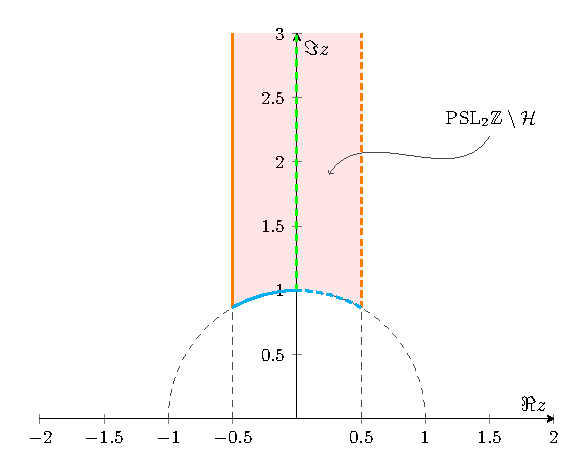
\includegraphics[scale=0.7,angle=0]{psl2.pdf}
  \noindent\\
  \decoRule
  \caption{Fundamental domain of modular surface.}
  \label{fig:fund_dom_psl2}
\end{figure}



At the link \url{https://roywilliams.github.io/play/js/sl2z/} it is possible to find a visualisation of point-orbits on the tassellation of the plane induced by $\PSL_{2}\Z$.

\begin{nese}[Bolza surface]
\label{ese:bolza_surface}
The \emph{modular surface} is the quotient $\Gamma\setminus\Hilb$ where $\Gamma=\PSL_{2}\Z$. The group $\PSL_{2}\Z$ is generated by the two matrices
\[
g_{k}=\Qmatrix{
1+\sqrt{2} & (2+\sqrt{2})\alpha\e^{\imi\frac{k\pi}{4}}\\
(2+\sqrt{2})\alpha\e^{-\imi\frac{k\pi}{4}} & 1+\sqrt{2}
},\quad\alpha=\sqrt{\sqrt{2}-1},\forall k=0,\ldots,7.
\]
\end{nese}

\begin{figure}[H]
\centering
  %
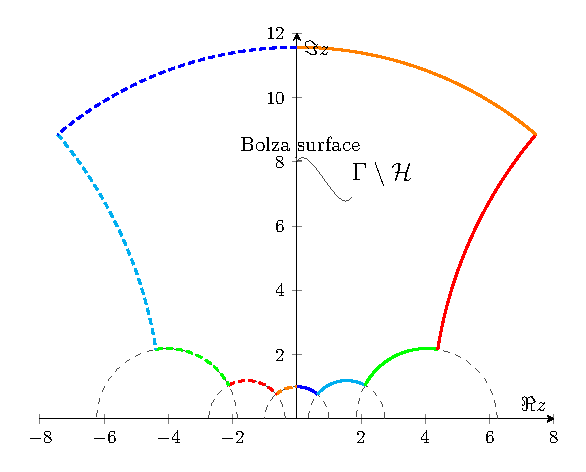
\includegraphics[scale=0.8,angle=0]{bolza_H.pdf}
  \noindent\\
  \decoRule
  \caption{Fundamental domain of bolza surface in $\Hilb$.}
  \label{fig:fund_dom_bolza_h}
\end{figure}

Considering the Dirichlet domain centered in $\Disk\ni z=0$, a fundamental domain for the Bolza surface is given by the hyperbolic octagon with vertices at point $2^{-1/4}\exp\left(\imi\left(\frac{\pi}{8}+\frac{k\pi}{4}\right)\right)$ for $k=0,\ldots,7$, with opposite sides identified.

\begin{figure}[H]
\centering
  %
  \begin{subfigure}[b]{0.4\textwidth}
  \centering
    
\includegraphics[scale=0.1,angle=0]{Bolza_cover238.jpg}
    %\caption{Variabili $X_{n}$}
    \label{fig:bolza_238}
  \end{subfigure}
  \begin{subfigure}[b]{0.36\textwidth}
  \centering
    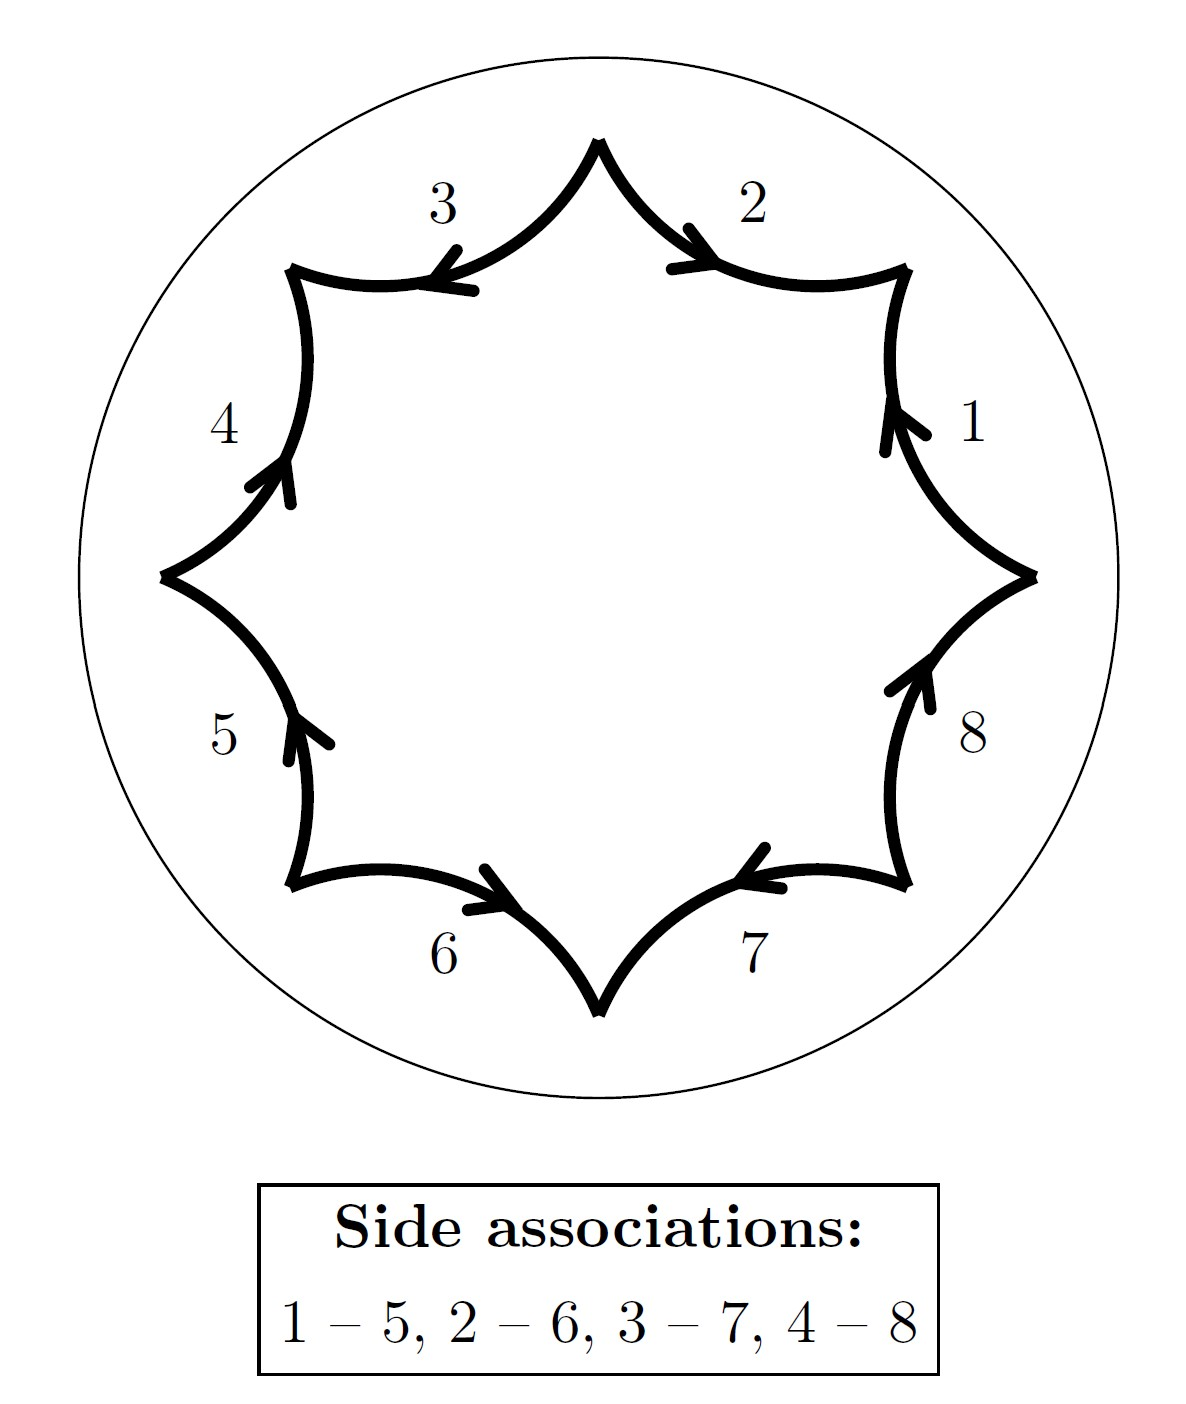
\includegraphics[scale=0.2,angle=0]{bolza_pair.jpg}
    %\caption{Variabili $X_{n}$}
    \label{fig:sides_bolza}
  \end{subfigure}
  \noindent\\
  \decoRule
  \caption{Bolza surface fundamental domain as subgroup of triangle group $\triang(2,3,8)$ (on the left) and with sides identification (on the right).}
  \label{fig:oval_card_orbits}
\end{figure}


There are two interesting facts about Fuchsian groups, which we will not prove (\cite{Katok:groups}).

\begin{defin}
\label{def:lattice}
A discrete subgroup $\Gamma<\PSL_{2}\R$ is a \emph{lattice} if it has a fundamental domain $D$ of finite area.
\end{defin}


\begin{nteo}[Siegel]
\label{teo:siegel}
If $\Gamma$ is a lattice, then any Dirichlet fundamental domain has finitely many sides.
\end{nteo}

\begin{nteo}
If $\Gamma$ is co-compact, i.e. the quotient $\Gamma\setminus\Hilb$ is compact, then $\Gamma$ has no parabolic element.
\end{nteo}

The rationale behind this result is that, is the quotient is compact, then it does not have point at extended real axis $\R\cup\{\infty\}$, so it cannot have parabolic elements whose fix elements lie on $\R\cup\{\infty\}$.








\section{Hyperbolic dynamics}


\label{sec:hyp_dynam}

\subsection{Geodesic flow}

The description given above can be regarded as a sort of \virg{discrete} motion induced by $A\in\PSL_{2}\R$ on a point of the unit tangent bundle $(z,\tau)\in T^{1}\Hilb$. So, the following question would be how to describe the continuos motion of a point $z$, given a direction $\tau$. This can be achived by the notion of \emph{geodesic flow}.

\begin{defin}
\label{def:geod_flow}
The \emph{geodesic flow} is a one parameter family of maps 
\[
a_{t}\colon T^{1}\Hilb\to T^{1}\Hilb
\]
for $t\in\R$, such that for any $(z,\tau)\in T^{1}\Hilb$ and $(\gamma(t),\gamma'(t))=a_{t}(z,\tau)$ is the unique geodesic parametrised by the \emph{arc length} satisfying $\gamma(0)=z,\gamma'(0)=\tau$.
\end{defin}

In the previous section, we have shown that, for each point $(z,\tau)$ there exist one and only and element $G\in\PSL_{2}\R$ such that $G(\imi,\imi)=(z,\tau)$, which is explicity given by equation \eqref{eq:main_matrix}. So the problem of parameterizing the geodesic starting from $z$ with direction $\tau$ can be brought back of parametrizing the geodesic starting from $\imi$ with direction $\imi$. However, we already now that this one is the vertical line $\imi t$ and an arc-length parametrization is given by $\imi\e^{t}$. In particular, we have that 
\begin{align*}
A_{t}(\imi,\imi)&=\Qmatrix{\exp(t/2)&\\&\exp(-t/2)}(\imi,\imi)\\
&=\left(\frac{\exp(t/2)\imi}{\exp(-t/2)},\frac{\imi}{(0+\exp(-t/2))^{2}}\right)=(\exp(t)\imi,\exp(t)\imi)
\end{align*}
which is the desired parametrization. Hence, for any $(z,\tau)\in T^{1}\Hilb$, if $G\in\PSL_{2}\R$ is such that $G(\imi,\imi)=(z,\tau)$, we have that
\[
a_{t}(z,\tau)=GA_{t}(\imi,\imi).
\]

In particular, recalling the Iwasawa decomposition \ref{impTeo:iwasawa}, via the identification of lemma \ref{lem:t1h_psl2_identification}, the geodesic flow is the right action of one parameter family 
\[
\Lie{A}=\left\{A_{t}=
\Qmatrix{\exp(t/2)&\\&\exp(-t/2)},\quad t\in\R
\right\}
\]
on the total group $\PSL_{2}\R$. There are other two fundamental flows on $T^{1}\Hilb$, corrisponding to different one parameter subgroups of $\PSL_{2}\R$. One is the (\emph{stable}) \emph{\textbf{horocycle flow}} by the one parameter subgroup
\[
\Lie{U}=\Lie{U}^{+}=\left\{
U_{t}=\Qmatrix{1&t\\&1},\quad t\in\R
\right\}
\]
and the other one is the \emph{unstable horocycle flow} given by 
\[
\Lie{U}^{-}=\left\{
U_{t}=\Qmatrix{1&\\t&1},\quad t\in\R
\right\}
\]
In figure \ref{fig:hyp_action_flows} it's possible to see the simultaneous action of the three groups on the point $(\imi,\e^{\imi\pi/3})$.

\begin{figure}[H]
\centering
  %
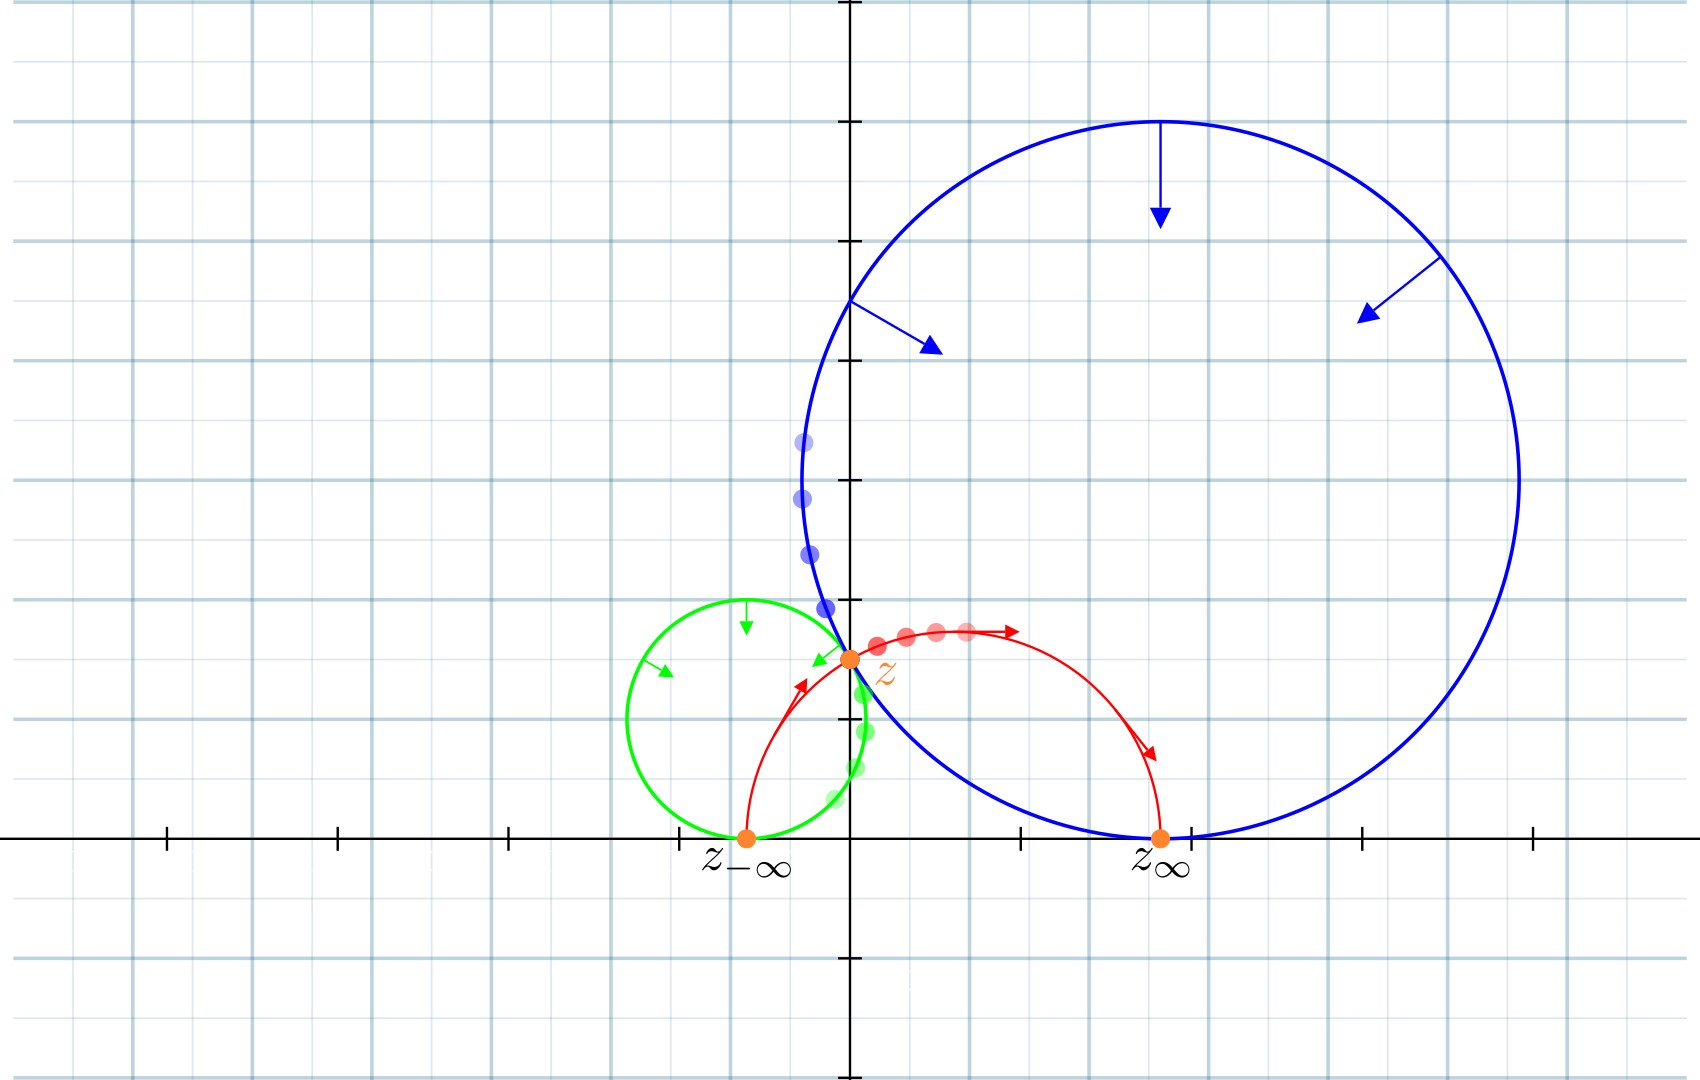
\includegraphics[scale=0.2,angle=0]{Flows.jpg}
  \noindent\\
  \decoRule
  \caption{Action of geodesic, stable and unstable horocycle flow.}
  \label{fig:hyp_action_flows}
\end{figure}



\subsection{Mixing flow on hyperbolic plane}

\label{subsec:mixing}

The area form on $\Hilb$ 
\[
\dd A=\frac{\dd x\wedge\dd y}{y^{2}}
\]
and the volume form on $T^{1}\Hilb\simeq\PSL_{2}\R$
\[
\dd V=\frac{\dd x\wedge\dd y\wedge\dd\theta}{y^{2}}
\]
are both invariant with respect to the action of the geodesic flow and horocycle flows, by virtue of theorem \ref{teo:area_volume_forms_invariants_isometries}, so it's interesting to study the corrisponding metric system.

We recall the notion of ergodic and mixing dynamical systems \ref{def:ergo_mix_continuos_system} (regarding the case of interest, we will use the continuos-case definitions). 

\begin{defin}
\label{def:ergo_mix_continuos_system}
Let $(X,\mathcal{X},\mu,R_{t})$ a continuos metric dynamical system (in particular $R_{t\ast}\mu=\mu\,\forall t\in\R$). Then:
\begin{itemize}
\item the flow $R_{t}$ is \emph{\boldsf{ergodic}} if for every measurable set $B\subset X$ which is $R_{t}$ invariant, $\mu(B)=0$ or $\mu(X\setminus B)=0$;
\item the flow $R_{t}$ is \emph{\boldsf{mixing}} if for every measurable sets $B,C\subset X$ 
\[
\mu(B\cap R_{t}^{-1}[C])\to\mu(B)\mu(C)
\]
holds, when $t\to\infty$.
\end{itemize} 
\end{defin}

These notions describes different manifestations of chaotich behaviour for a classical dynamical system. In particular, the mixing property is stronger than ergodic one: ergodicness of a system only assure that, in certain sense, that for a.e. point the orbit will go through all over the space $X$; on the other hand, mixing property regards how much a system \virg{mixes} itself. We will prove the following.

\begin{nteo}
\label{teo:geod_horo_are_mixing}
The geodesic and horocyclic flows are mixing.
\end{nteo}

This theorem is a direct consequence of a more general result about matrix coefficients of representations of subgroups of $\SL_{2}\R$. A unitary representation of a group $G$ on a Hilbert space $H$ is a group homomorphism
\[
\pi\colon G\to\U(H)
\]
where $U(H)$ denotes the group of unitary transformations. This representation is \emph{strongly continuos} if, for any $\vphi\in H$, the map $g\mapsto\pi(g)\vphi$ is continuos. 
\begin{defin}
Given $\vphi,\psi\in H$, the function $g\mapsto\pscl{\pi(g)\vphi}{\psi}$ is called a \emph{\textbf{matrix coefficient}} of the representation.
\end{defin}
In our situation, $\pi$ will be a representation of the group $G=\SL_{2}\R$ action on the Hilbert space $H=L_{2}(X)$ with $X=\Gamma\setminus G$, defined by 
\[
\pi(g)\vphi(h)=\vphi(gh),\quad\forall g\in G,\vphi\in L_{2}(X).
\]
In our context, the above definitions of ergodicity and mixing can be translated as follows.

\begin{defin}
Let $\Lie{U}_{t}$ be a one parameter subgroup of $\SL_{2}\R$.
\begin{compactitem}
\item The flow associated to $\Lie{U}_{t}$ is \emph{ergodic} if and only if for any $t\in\R$, $\pi(\Lie{U}_{t})$ has no non-trivial invariant vector.
\item The flow associated to $\Lie{U}_{t}$ is \emph{mixing} if and only if for any $\vphi,\psi\in L_{2}(X)$,
\[
\pscl{\pi(\Lie{U}_{t})\vphi}{\psi}\to \int_{X}\vphi\dd\mu\int_{X}\psi\dd\mu
\]
for $t\to\infty$.
\end{compactitem}
\end{defin}

The general result from which we will get the mixing of the geodesic flow is then.

\begin{impTeo}{Howe-Moore}{mixing_flow_psl2}
%\label{teo:mixing_flow_psl2}
Let $\pi$ be a strongly continuos unitary representation of $\SL_{2}\R$ on a Hilbert space $\Hilb$. Assume that $\pi$ has non-trivial invariant vector in $\Hilb$. Then, if $G_{n}$ is a diverging\footnote{That is for any compact $K\subset \SL_{2}\R$, there exists $N\in\N$ such that $G_{n}\not\in K$ for all $n\geq N$.} sequence in $\SL_{2}\R$, then 
\[
\lim_{n\to\infty}\pscl{\pi(G_{n})\vphi}{\psi}=\int_{X}\vphi\dd\mu\int_{X}\psi\dd\mu
\]
\end{impTeo}
\begin{prf}
See \ref{teo:mixing_flow_psl2_appendix}, in Appendix \ref{AppendixA}.
\end{prf}

In fact, in our case, the group $\SL_{2}\R$ acts transitively on $X$, so, if $f$ a invariant vector with respect to $\SL_{2}\R$, it must be constant, hence $\pi$ has no trivial invariant vector. The geodesic flow and the horocycle flow are given by the action of matrices $A_{t}$ and $U_{\pm t}$. In both cases, we are given a diverging sequence and so we are done.\\
\noindent\\
A mentioned in chapter \ref{Chapter1}, this is only a particular case of the more general result due to the Hopf, roughlt stated in \ref{teo:Hopf_theorem}.

\begin{impTeo}{Hopf}{hopf_ergodic}
%\ref{impTeo:hopf_ergodic}
Let $(M,g)$ be a compact Riemannian manifold with negative sectional curvature. Then the geodesic flow $\Phi_{t}\colon TM\to TM$ is ergodic.
\end{impTeo}


\subsection{Examples}


Although the geodesic flow on an hyperbolic surface is indeed ergodic, this does not prevent the existence of some periodic orbits. Nonetheless, these periodic orbits are very unstable, and little differences in initial condition produces very different behaviour during time evolution.



\begin{figure}[H]
\centering
  %
  \begin{subfigure}[b]{0.3\textwidth}
  \centering
    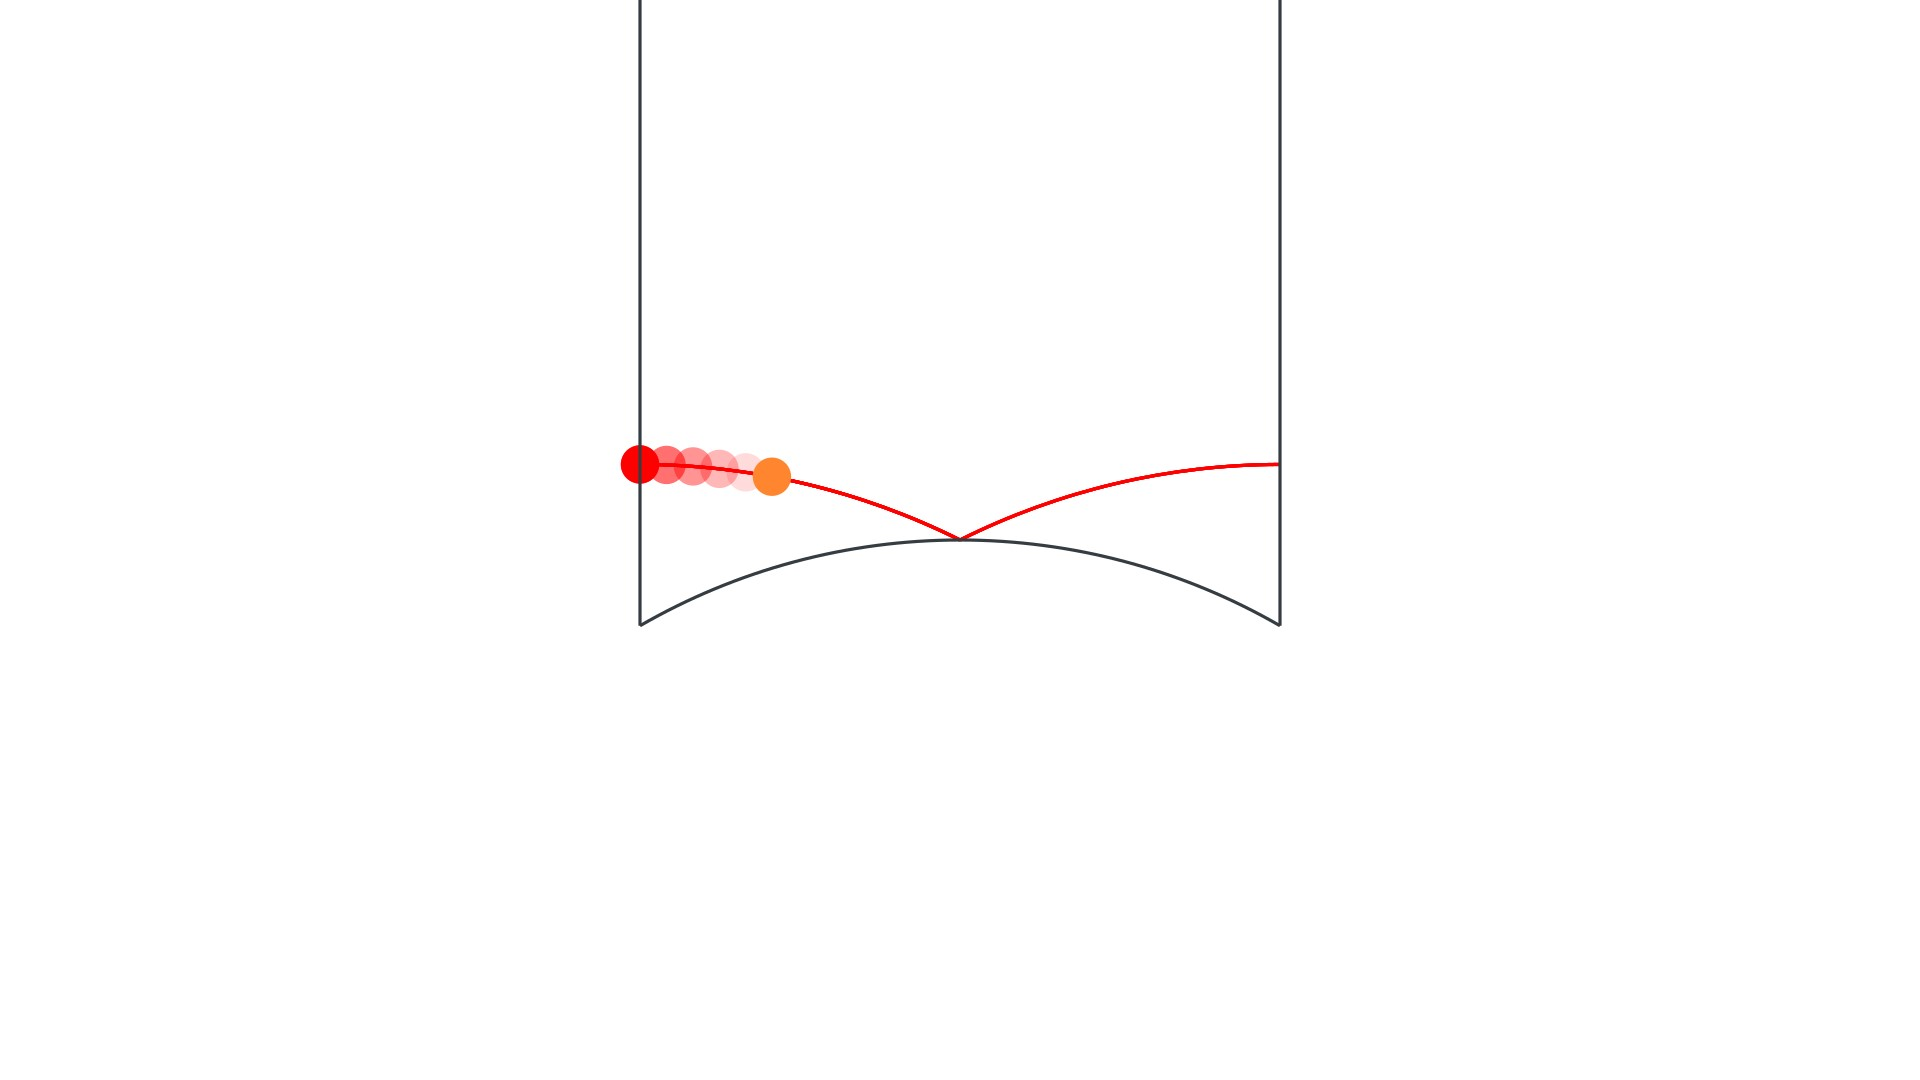
\includegraphics[scale=0.1,angle=0]{Periodic1.jpg}
    %\caption{Variabili $X_{n}$}
    \label{fig:mod_period_1}
  \end{subfigure}
  \begin{subfigure}[b]{0.3\textwidth}
  \centering
    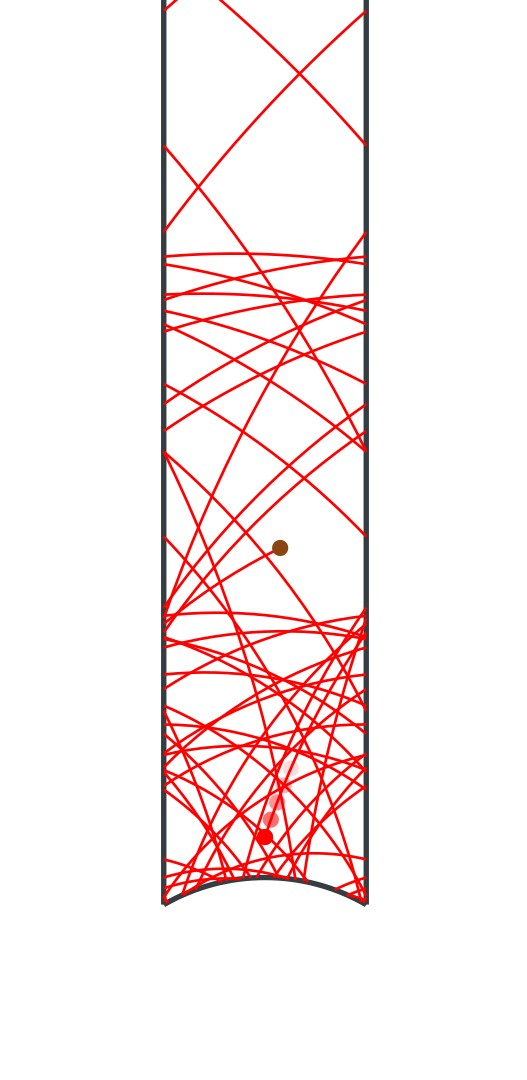
\includegraphics[scale=0.12,angle=0]{modular_billiard.jpg}
    %\caption{Variabili $X_{n}$}
    \label{fig:mod_erg}
  \end{subfigure}
    \begin{subfigure}[b]{0.3\textwidth}
  \centering
    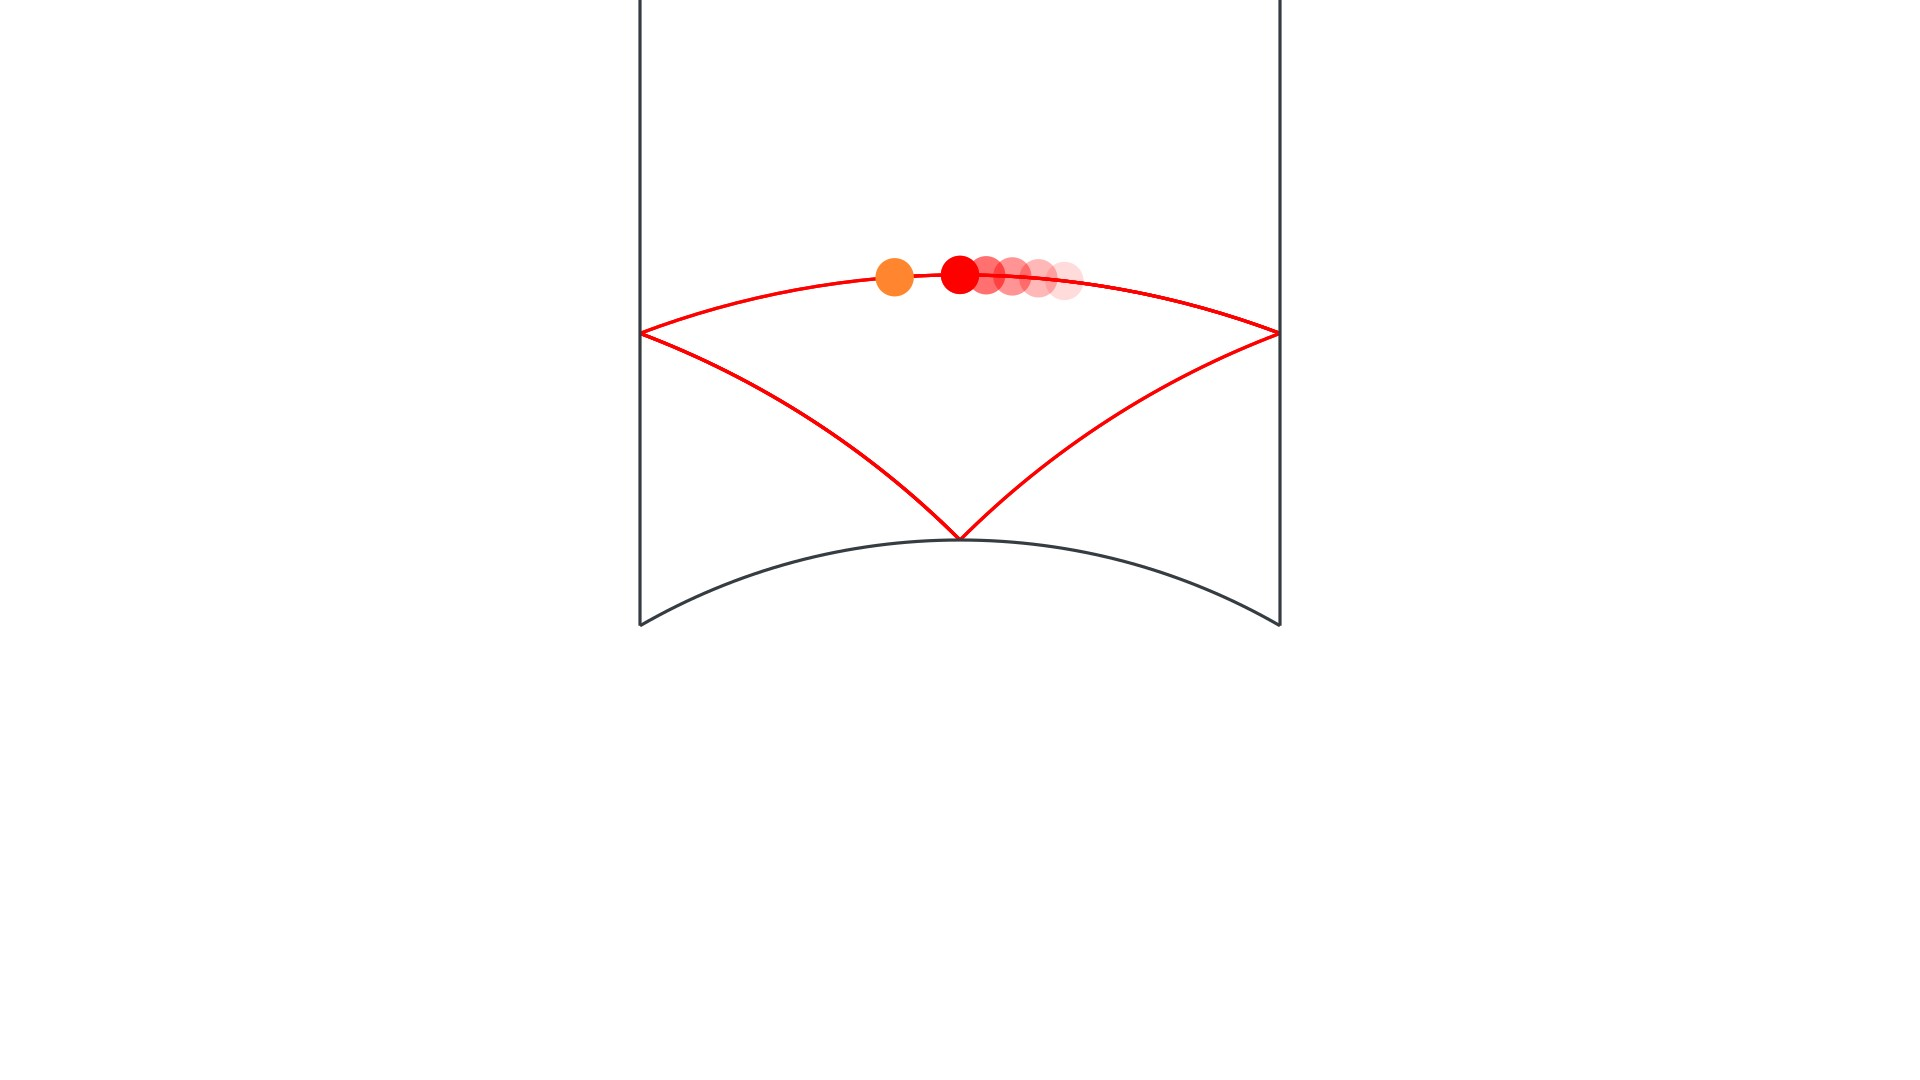
\includegraphics[scale=0.1,angle=0]{Periodic2.jpg}
    %\caption{Variabili $X_{n}$}
    \label{fig:mod_period_2}
  \end{subfigure}	
  \noindent\\
  \decoRule
  \caption{A typical chaotical orbit on the modular surface (in the center), along with two periodic orbits.}
  \label{fig:modular_orbits}
\end{figure}


As seen at the end of section \ref{subsec:hyp_isom}, hyperbolic elements $A\in\PSL_{2}\R$ have a fixed geodesic, which is its \emph{axis}. We can see periodic orbits on the modular surface as axis of particular hyperbolic elements, see also section \ref{sec:period_geodesics}. The two periodic orbits (of periods $4$ and $6$) in figure \ref{fig:modular_orbits} are given by the two matrices:
\begin{align*}
A_{l}=\frac{1}{2}\Qmatrix{5^{1/4}-5^{-1/4}&-(5^{1/4}-5^{-1/4})\\
2/5^{1/4}&2/5^{1/4}}&\colon\text{ figure on the left}\\
A_{r}=\frac{1}{6}\Qmatrix{3\sqrt{2}\sqrt[4]{3}&-3\sqrt{2}\sqrt[4]{3}\\
\sqrt{2}3^{3/4}&\sqrt{2}3^{3/4}}&\colon\text{ figure on the right}
\end{align*}


Using the \emph{Klein $j$-function}\footnote{It is the unique modular function of weight zero for $\SL_{2}\Z$, such that it is holomorphic away from the cusp (where )}, it is possible to visualize the above motions on the hyperbolic surface on the sphere, getting the images \ref{fig:modular_orbits_3d} (in it are visualized the periodic orbit of matrix $A_{r}$ and the above ergodic one).


\begin{figure}[H]
\centering
  %
  \begin{subfigure}[b]{0.3\textwidth}
  \centering
    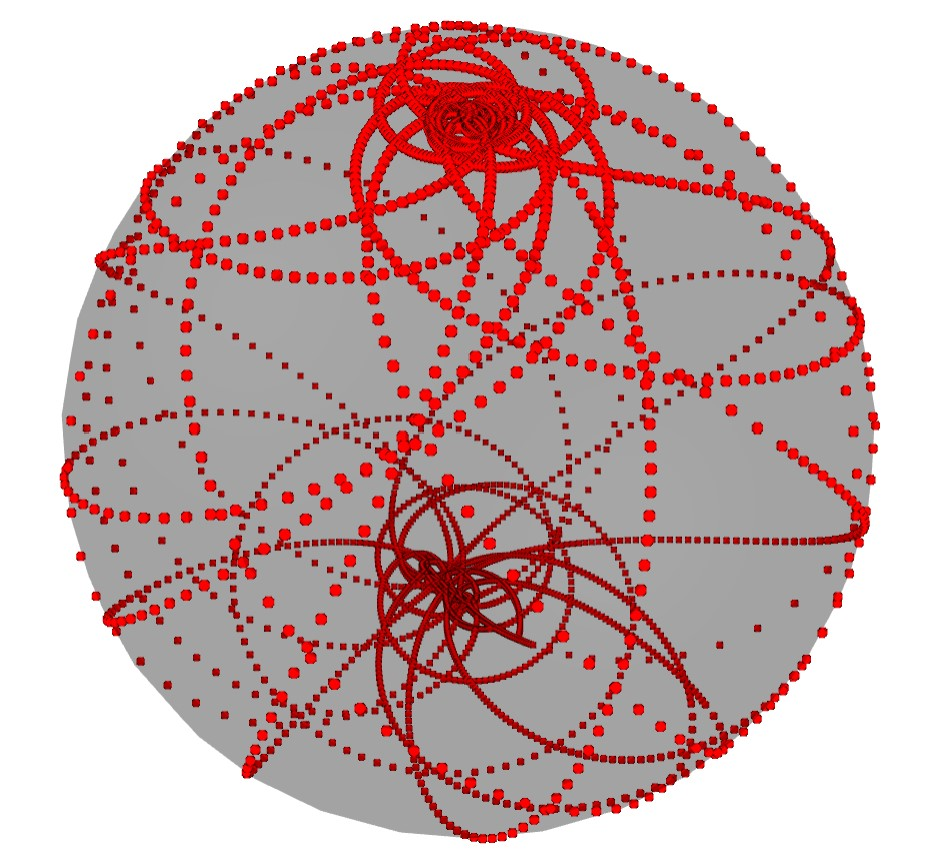
\includegraphics[scale=0.25,angle=0]{Orbit3D.jpg}
    %\caption{Variabili $X_{n}$}
    \label{fig:mod_3d_erg}
  \end{subfigure}
  \begin{subfigure}[b]{0.3\textwidth}
  \centering
    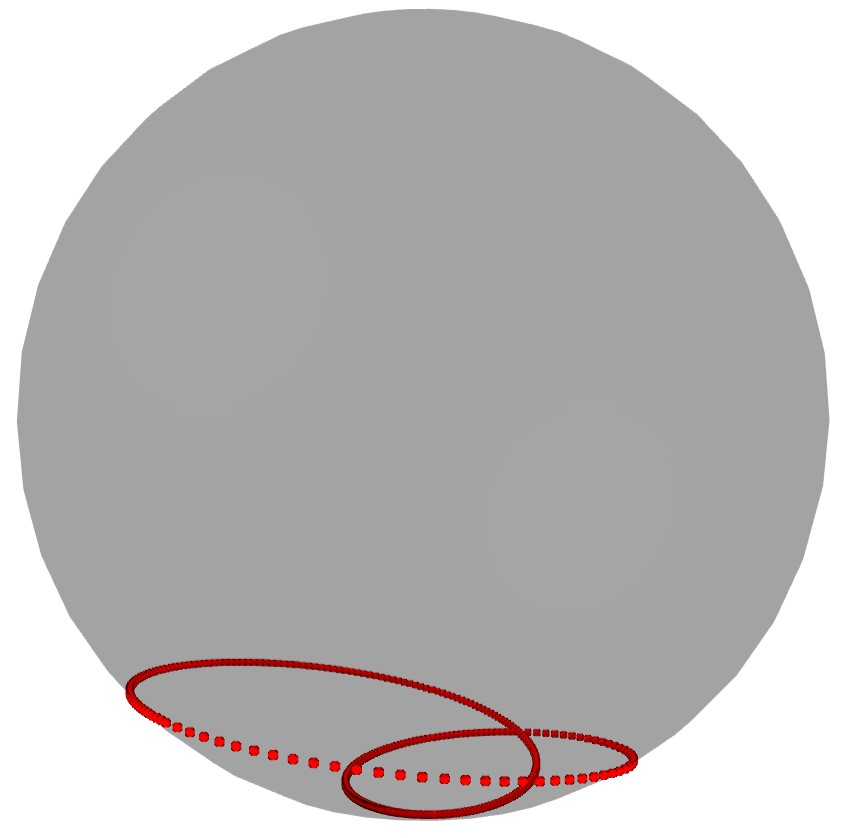
\includegraphics[scale=0.25,angle=0]{Orbit3Dperiod.jpg}
    %\caption{Variabili $X_{n}$}
    \label{fig:mod_3d_period}
  \end{subfigure}
  \noindent\\
  \decoRule
  \caption{3D visualisation of motion on hyperbolic surface.}
  \label{fig:modular_orbits_3d}
\end{figure}


%-----------------------------------
%	SUBSECTION 1
%-----------------------------------


%-----------------------------------
%	SUBSECTION 2
%-----------------------------------

%----------------------------------------------------------------------------------------
%	SECTION 2
%----------------------------------------------------------------------------------------

\section{Spectra of modular surfaces}

The modular group $\SL_{2}\Z$ has a particular importance in among the fuchsian groups, even if it (or better, its quotient $\PSL_{2}\Z$) can be seen just as a triangular group. This group has lots of arithmetic properties and for this reason it has been widely study, starting from its \emph{\textbf{principal congruence subgroups}} of level $N$ defined by
\begin{equation}
\label{eq:subgroups_congruence}
\Gamma(N)=\left\{
G\in\SL_{2}\colon G\equiv_{N}I
\right\}
\end{equation}
where the congruence \virg{$\equiv$} is taken componentwise. In general, a congruence subgroup of $\Gamma(1)=\SL_{2}\Z$ is a subgroup $\Gamma\leq\SL_{2}\Z$ for which there exists an $N$ such that $\Gamma\geq\Gamma(N)$ (roughly speaking, it is an \virg{upper subgroup of a principal congruence subgroup}).\\
The \emph{modular surface of level $N$} is then defined as
\begin{equation}
X(N)\coloneqq \Gamma(N)\setminus\Hilb.
\end{equation}
It is, for all $N\geq1$, a finite-area, non-compact hyperbolic surface. Just to emphasize the relevance of this subgroups, it can be shown that $X(1)$, with its complex structure, can parametrize the space of elliptic curves over $\mathbb{C}$, \cite{Shimura:book}.\\ %sanrak pg 3

Topologically speaking, the principal modular surface $X(1)$ is a like-sphere surface, with the hyperbolic metric and three \virg{cusp}. Moreover, its hyperbolic surface is equal\footnote{It is possible to use Gauss-Bonnet formula, which states that the hyperbolic area of a $\triang(a,b,c)$ is equal to $\pi(1-1/a-1/b-1c)$.} to $\pi/3$. To link the next chapter, we can now present the problem of our interest, which is the \virg{quantum-eigenvalue} problem

\begin{equation}
\label{eq:lapl_eingev_probl_hyp_surface}
\begin{cases}
\Lapl\vphi+\lambda\vphi&=0\\
\vphi(Gz)=\vphi(z)&;\forall G\in\Gamma\\
\int_{\Gamma\setminus\Hilb}\abs{\vphi}^{2}\dd\mu &<infty
\end{cases}
\end{equation}
with $\Gamma$ fuchsian group, in particular are extremly important the principal congruence subgroups $\Gamma(N)$. As we will see, the existence of a solution of the problem \ref{eq:lapl_eingev_probl_hyp_surface} is granted if the quotient space $X$ is compact, which is not the case for subgroups $X(N)$. This matter will be discussed in chapter \ref{Chapter6}. Avoiding the existence problem, solutions of problem \ref{eq:lapl_eingev_probl_hyp_surface} are called \emph{Maass forms}. 











% Chapter Template

\chapter{Semiclassical analysis} % Main chapter title

\label{Chapter2} % Change X to a consecutive number; for referencing this chapter elsewhere, use \ref{ChapterX}
\thispagestyle{empty}
%----------------------------------------------------------------------------------------
%	SECTION 1
%----------------------------------------------------------------------------------------

In this chapter we provide a very brief introduction to basic notions of semiclassical analysis, in particular about symbol quantization. The tools of semiclassical analysis will be essential to understand Weyl's law and the important Egorov theorem. A comprehensive resource for this subject is \cite{Zworski:semic}, but for a general introductive overview the lecture notes \cite{Semy:lec_semi} can be very helpful.


\section{Semiclassical Quantizazion}

To be able to relate classical mechanics and its quantum counterpart it is necessary to associate the Hilbert space $H=L^{2}(M)$ (where $M$ is a manifold) to the mathematical basic structure for classical mechanics, i.e. the cotangent bundle $T^{\ast}M$ with its symplectic structure. Moreover, it is necessary to associate operators on $H$ to functions on $T^{\ast}M$.\\
From a functorial \virg{universal} point of view, there is no procedure to do this \cite{Hove:noFunc}, but there are practical standard and useful ways to do so. One of the most convenient is \emph{Weyl quantization}, which associate classical quantities (\emph{symbols}) $a(x,p)\colon T^{\ast}M\to\mathbb{C}$ to a quantum observable (pseudodifferential operator) $A(x,\planck\Diff)$, where $x$ is still the position, but $\Diff$ is a differential and $\planck$ is a (semiclassical) parameter. In this sense, the limit $h\to0$ is to be understood as the classical limit, from the quantum level and for this reason is called \emph{semiclassical limit}. We will now provide the basic notions of this approach.



\subsection{Semiclassical Fourier transform}

From elementary physics, we know that Fourier transform allows us to \virg{change} functions of the position variable $q$ to functions of the momentum $p$, in the phase space $T^{\ast}M$. Quantization is the tool that allows us to deal with both sets of variables simultaneously in the semiclassical limit. Functions of both $q$ and $p$ variables are called symbols, and are quantized using a sort of \virg{semiclassical Fourier transform}.\\

We refer to appendix \ref{Appendix_Fourier} for the details about classical Fourier transform and the theory of distributions. The latter is a class of important functions related to Fourier transform, in particular we consider the set of \emph{tempered distribution}, which can be view as the dual (in the sense of vector spaces) of Schwarz space $\schwarz$ defined by 
\[
\schwarz=\left\{
f\in C^{\infty}(\R^{n})\colon \norm{}_{\alpha,\beta}<\infty
\,\forall\alpha,\beta\in\N^{n}\right\},
\]
where $\norm{\cdot}_{\alpha,\beta}$ is the seminorm defined in \ref{def:scwharz_space}. In other words, Schwarz space $\schwarz$ is the set of smooth functions with \virg{rapid decay}. Just to understand the importance of Fourier transform in physics, we will show how it provides the mathematical fundation for the Heisenberg uncertainty principle \cite{DU:notes}.


\begin{nese}[Heinsenberg uncertainty principle in $\R$]
\label{ese:heisenberg_fourier}
Consider some $\psi\in L^{2}(\R)$ where $x\psi$ and $p\Fourier(\psi)\in L^{2}(\R)$. With the dispersion of $\psi$ defined as
\[
\mathcal{D}\psi\coloneqq\frac{\int_{\R}x^{2}\abs{\psi(x)}^{2}\dd x}{\int_{\R}\abs{\psi(x)}^{2}\dd x},
\]
we will show, through straightforward computation, that 
\[
(\mathcal{D}\psi)(\mathcal{D}\Fourier(\psi))\geq\frac{1}{4}.
\]
By integration by parts, we get
\begin{align*}
\int_{\R}\abs{\psi(x)}^{2}\dd x &= \left.x\abs{\psi(x)}^{2}\right|_{-\infty}^{\infty}-\int_{\R}x\psi(x)\overline{\psi'(x)}\dd x-\int_{\R}x\overline{\psi(x)}\psi'(x)\dd x\\
&=-2\Re\left(
\int_{\R}x\overline{\psi(x)}\psi'(x)\dd x
\right),
\end{align*}
where the first term is vanished from the decay properties of functions in $\schwarz$. Squaring both sides and using Schwarz inequality gives 
\[
\left( 
\int_{\R}\abs{\psi(x)}^{2}\dd x
\right)^{2}\leq 4
\left(\int_{\R}\abs{x\overline{\psi(x)}\psi'(x)}\dd x\right)^{2}\leq 4\left(\int_{\R}x^{2}\abs{\psi(x)}^{2}\dd x\right)\left(
\int_{\R}\abs{\psi'(x)}^{2}\dd x
\right).
\]
(i) and (iv) of proposition \ref{prop:prop_of_fourier} give $\Fourier(\psi'(x))=\imi p\Fourier(\psi)(p)$ and $\norm{\psi}^{2}=(2\pi)^{-1}\norm{\Fourier(\psi)}^{2}$, so
\[
\int_{\R}\abs{\psi'(x)}^{2}\dd x = \frac{1}{2\pi}\int_{\R}p^{2}\abs{\Four{\psi}(p)}^{2}\dd p.
\]
The thesis follows by last two equalities.
\end{nese}

This simple yet fundamental example is explanatory of the following definition, i.e. the semiclassical Fourier transform. 

\begin{defin}[semiclassical Fourier transform]
For a parameter $\planck>0$, the semiclassical Fourier transform $\Fourier_{\planck}\colon\schwarz'\to\schwarz'$ is defined by
\[
\Fourier_{\planck}(f)(p)\coloneqq\Fourier(f)\left(\frac{p}{\planck}\right)=\int_{\R^{n}}\e^{-\frac{\imi}{\planck}\pscl{q}{p}}f(q)\dd q,
\]
with the inverse 
\[
\Fourier_{\planck}^{-1}(f)(q)=\planck^{-n}\Fourier(f)\left(
\frac{q}{\planck}
\right)=\frac{1}{(2\pi\planck)^{n}}\int_{\R^{n}}\e^{\frac{\imi}{\planck}\pscl{q}{p}}f(p)\dd p.
\]
\end{defin}

This different version of Fourier transform has lots of properties similar to the ones of the classical version (see proposition \ref{prop:four_properties}).

\begin{nprop}
\label{prop:properties_semicl_fourier}
\begin{compactenum}
\item $(\planck\Diff_{p})^{\alpha}\Fourier_{\planck}(\vphi)=\Fourier((-q)^{\alpha}\vphi)$ and $\Fourier_{\planck}((\planck\Diff_{q})^{\alpha}\vphi)=p^{\alpha}\Fourier_{\planck}(\vphi)$.
\item $\norm{\vphi}=(2\pi\planck)^{-n/2}\norm{\Fourier_{\planck}(\vphi)}$.
\end{compactenum}
\end{nprop}
\begin{prf}
See \cite{Zworski:semic}.
\end{prf}

The aim behind this definition is the desire to control the degree of localization and uncertainty of $\Fourier$ in the semiclassical limit, using a parameter $h>0$. This is the statement of subsequent theorem \ref{teo:new_uncert_principle}.


\begin{nteo}[generalized uncertainty principle]
\label{teo:new_uncert_principle}
For $j=1,\ldots,n$ and $f\in\schwarz'$, it holds
\[
\frac{\planck}{2}\norm{f}\cdot\norm{\Fourier_{\planck}(f)}\leq \norm{q_{j}f}\cdot \norm{p_{j}\Fourier_{\planck}(f)}.
\]
\end{nteo}
\begin{prf}
See \cite{Zworski:semic}.% th 2.1.13 WONG 
\end{prf}

The foregoing theorem \ref{teo:new_uncert_principle} generalizes the previous example \ref{ese:heisenberg_fourier}. It can be retrived from theorem \ref{teo:new_uncert_principle} by choosing $n=1$ and $\planck=1/2$. In particular, we can do the following reasoning. Suppose that, in general, we have a function $\psi\in L^{2}(\R^{n})$ where $1=\norm{\psi}=(2\pi\planck)^{-n/2}\norm{\Fourier_{\planck}(\psi)}$.\\
As before, the localization of $\psi$ relative to $x=0$ can be gauged by $\norm{q_{j}\psi}$ for $j=1,\ldots,n$. For example, suppose that
\[
\psi(q)=\planck^{-\norm{\alpha}_{1}/2}\phi(q_{1}/\planck^{\alpha_{1}},\ldots)
\]
for some $n$-uple of positive real numbers $\alpha$, with $\norm{\alpha}_{\infty}\leq 1$, $\phi\in\schwarz$ and $\norm{\phi}=1$. Then, with some computations, it is possible to prove  (CITA \cite{Zworski:semic})
\[
\int_{\R^{n}-N_{\planck}(\veps)}\abs{\psi(x)}^{2}\dd x
\]
is \virg{very small}, where $N_{h}(\veps)\coloneqq\prod_{i=1}^{n}[-\planck^{\alpha_{i}-\veps},\planck^{\alpha_{i}-\veps}]$. Moreover, $\norm{x_{j}\psi}\simeq \planck^{\alpha_{j}}$, for all $j$. On the other hand, the semiclassical Fourier transform gives us 
\[
\Fourier_{\planck}(\psi)(p)=\planck^{\norm{\alpha}_{1}/2}\Fourier(\psi)(p_{1}/\planck^{1-\alpha_{1}},\ldots,p_{n}/\planck^{1-\alpha_{n}}),
\]
which implies that $(2\pi\planck)^{-n/2}\norm{p_{j}\Fourier_{\planck}(\psi)}\simeq \planck^{1-\alpha_{j}}$. Again, the localization in $q$ is matched by delocalization in $p$, and vice-versa.


\subsection{How to quantize}

\label{subsec:how_to_quant}

We will now write down quantization formulas, which are equations that let us associate symbols (classical observables) to $\planck$-dependent linear operators (quantum observables) which acts on functions $\vphi(x)\in\schwarz(\R^{n})$. We will use variable $x$ for position coordinates, rather than general variable $q$.

\begin{defin}[symbols and Weyl-quantization]
Any function $a=a(x,p)\in\mathcal{S}(\R^{2n})$ in the Schwartz space will be called \emph{symbol}. The \emph{Weyl quantization}
\[
\Op^{W}\colon\schwarz(\R^{2n})\to\Hom(\schwarz(\R^{n}))
\]
of symbol $a$ is defined by
\begin{equation}
\label{eq:weyl_quant_symbol}
\Op^{W}(a)(\vphi)(x)=\frac{1}{(2\pi\planck)^{n}}\int_{\R^{n}}\int_{\R^{n}}\e^{\frac{\imi}{\planck}\pscl{x-y}{p}}\, a\left(\frac{x+y}{2},p\right)\vphi(y)\dd y\dd p,
\end{equation}
where $\vphi\in\schwarz(\R^{n})$.
\end{defin}


\begin{remark}[\emph{Semiclassical pseudodifferential operator}]
\label{def:semicla_opert_in_remark}
It's possible to define a generalization of Weyl quantization, i.e. the $t$-quantization for $0\leq t\leq1$, given by
\[
\Op_{t}(a)(\vphi)(x)=\frac{1}{(2\pi\planck)^{n}}\int_{\R^{n}}\int_{\R^{n}}\e^{\frac{\imi}{\planck}\pscl{x-y}{p}}\, a\left(tx+(1-t)y,p\right)\vphi(y)\dd y\dd p.
\]
The Weyl quantization is realized for $t=1/2$, while the \emph{left-right quantization} are obtained for $t=1,0$ respectively. The left quantization $\Op^{l}=\Op_{1}$ is often called \emph{standard quantization}.\\
In general, any operator of the form $\Op_{t}(a)$ is called a \emph{semiclassical pseudodifferential operator} and its dependency on both $x,\planck D$ is expressed by $\Op_{t}(a)(x,\planck D)$.
\end{remark}


In view of remark \ref{def:semicla_opert_in_remark}, we see that Weyl-quantization is a sort of \virg{mean} between left and right quantization (it is defined as $\Op_{1/2}$). The Weyl quantization has a number of useful properties.

\begin{nese}
\label{ese:weyl_sends_real_to_syummetric}
Let $a$ a real-valued function (symbol). Then $\Op^{W}(a)$ is a symmetric operator, i.e.
\[
\pscl{\Op^{W}(a)(\psi_{1})}{\psi_{2}}=\pscl{\psi_{1}}{\Op^{W}(a)(\psi_{2})}.
\]
For this,
\begin{align*}
\int\Op^{W}(a)(\psi_{1})(x)\overline{\psi_{2}(x)}\dd x&=
\iiint\e^{\frac{\imi}{\planck}\pscl{x-y}{p}}\, a\left(\frac{x+y}{2},p\right)\psi_{1}(y)\overline{\psi_{2}(x)}\dd x\dd y\dd p\\
&=\iiint\e^{\frac{\imi}{\planck}\pscl{x-y}{p}}\, \overline{a\left(\frac{x+y}{2},p\right)}\psi_{1}(y)\overline{\psi_{2}(x)}\dd x\dd y\dd p \\
&= \int\psi_{1}(y)\overline{\Op^{W}(a)(\psi_{2})(y)}\dd y.
\end{align*}
\end{nese} 

We will now briefly present some others examples of symbol quantization and some results that will be useful in the following sections (\cite{Zworski:semic}).

\begin{nese}[quantizing a $p$-dependent symbol]
If $a(x,p)=p^{{\alpha}}$ for a multiindex ${\alpha}\in\N^{n}$ , then we have
\[
\Op_{t}(a)(\vphi)(x)=a(x,\planck \Diff)\vphi(x)=(\planck \Diff)^{{\alpha}}\vphi(x) 
\]
where $\planck\Diff$ is a semiclassical scaling of the usual differential operator $\Diff^{{\alpha}}=i^{-\abs{{\alpha}}}\partial^{{\alpha}}$. If $a$ is \virg{polynomial} in $p$, with coefficients depending on $x$, i.e.
\[
a(x,p)=\sum_{\abs{{\alpha}}\leq N}\alpha_{{\alpha}}(x)p^{{\alpha}}
\]
we see why the operators created by quantization maps are called \virg{pseudodidifferential}: if $a$ is polynomial in $p$, we get a standard differential operator.
\end{nese}

\begin{nese}[quantizing a $x$-dependent symbol]
If $a(x,p)=a(x)$, then $\Op_{t}(a)(\vphi)=a\vphi$. To check this, we take the $t$-derivative of $\Op_{t}(a)(\vphi)$:
\begin{align*}
\partial_{t}\Op_{t}(a)(\vphi)&=
\frac{1}{(2\pi\planck)^{n}}\iint_{\R^{n}\times\R^{n}}\e^{\frac{\imi}{\planck}\pscl{x-y}{p}}\pscl{\partial_{t}a(tx+(1-t)y)}{x-y}\vphi(y)\dd y\dd p\\
&=\frac{\planck}{\imi(2\pi\planck)^{n}}\int_{\R^{n}}\Div_{p}\left(
\int_{\R^{n}}\e^{\frac{\imi}{\planck}\pscl{x-y}{p}}\partial_{t}a(tx+(1-t)y)\vphi(y)\dd y\right)\dd p\\
&=\frac{\planck}{\imi(2\pi\planck)^{n}}\int_{\R^{n}}\Div\left(\e^{\frac{\imi}{\planck}\pscl{x}{p}}\Fourier(\psi(p))\right)\dd p.
\end{align*}
where $\psi(y)=\partial_{t}a(tx+(1-t)y)\vphi(y)$. The last expression vanishes by rapid decay, and so $\Op_{t}(a)\vphi=\Op_{1}(a)\vphi=a\vphi$.
\end{nese}


\begin{nese}[quantizing a linear symbol]
\label{ese:quant_linear_symb}
Let $a(x,p)=\pscl{x}{\xi}+\pscl{p}{\rho}$ be a linear symbol. From the above examples, $\Op_{t}(a)=\pscl{x}{\xi}+\pscl{\planck\Diff}{\rho}$ for all $t\in[0,1]$.
\end{nese}


\begin{nprop}[Properties of quantization]
The followings hold:
\label{prop:quant_properties}
\begin{compactitem}
\item If $a\in\schwarz(\R^{2n})$, then $\Op_{t}(a)$ is a continous map from $\schwarz'(\R^{n})\to\schwarz(\R^{n})$ for all $t\in[0,1]$;
\item If $a\in\schwarz'(\R^{2n})$, then $\Op_{t}(a)$ is a continous map from $\schwarz'(\R^{n})\to\schwarz'(\R^{n})$ for all $t\in[0,1]$;
\item If $a\in\schwarz(\R^{2n})$, then the adjoint operator of $\Op_{t}(a)$ is $\Op_{1-t}(\bar{a})$: in particular the adjoint operator of the Weyl quantization of a real symbol is itself.
\end{compactitem}
\end{nprop}
\begin{prf}
See \cite{Martinez:semi}.
\end{prf}

\begin{nprop}
\label{prop:quant_commut}
% teo 2.1.20 wong
The followings hold:
\begin{compactitem}
\item $\Op^{W}(\Diff_{x_{j}}a)=[\Diff_{x_{j}},\Op^{W}(a)]$;
\item $\planck\Op^{W}(\Diff_{p_{j}}a)=-[x_{j},\Op^{w}(a)]$.
\end{compactitem}
\end{nprop}
\begin{prf}
Let $\vphi\in\schwarz$. We will prove the first statement, as the second is similar. Then by straightforward calculation
\begin{align*}
\Op^{W}(\Diff_{x_{j}}a)&=\frac{1}{(2\pi\planck)^{n}}\iint_{\R^{n}\times\R^{n}}\Diff_{x_{j}}a\left(\frac{x+y}{2},p\right)\e^{\frac{\imi}{\planck}\pscl{x-y}{p}}\vphi(y)\dd p\dd y\\
&=\frac{1}{(2\pi\planck)^{n}}\iint_{\R^{n}\times\R^{n}}(\Diff_{x_{j}}+\Diff_{y_{j}})a\left(\frac{x+y}{2},p\right)\e^{\frac{\imi}{\planck}\pscl{x-y}{p}}\vphi(y)\dd p\dd y
\end{align*}
\end{prf}

\begin{nprop}[conjugation]
% teo 2.1.21
\label{prop:semic_fourier_conj}
It holds
\[
\Fourier_{\planck}^{-1}\Op^{W}(a)(x,\planck\Diff)\Fourier_{\planck}=\Op^{W}(a)(\planck\Diff,-x).
\]
\end{nprop}
\begin{prf}
Omitted.
\end{prf}



\subsection{Semiclassical Pseudodifferential Operators}

From now on, we will only consider Weyl quantization for simplicity. The starting point is the equation
\begin{equation}
\label{eq:weyl_prod}
\Op^{W}(a)\Op^{W}(b)=\Op^{W}(c)
\end{equation}
for three symbols $a,b,c$. We want to know under which conditions this equation can hold and compute the corrispondent symbol $c$, which will be denoted by $c\coloneqq a\Wprd b$. So we define the \emph{Weyl product} of two symbols $a,b$ as a third symbol $c$ such that equation \eqref{eq:weyl_prod} holds.\\
A linear symbol is a function $l$ of the form 
\[
l(x,p)=\pscl{x}{\xi}+\pscl{p}{\rho}
\]
with $(\xi,\rho)\in\R^{2n}$ fixed. In this sense, there is a bijection between points of $\R^{n}$ and linear symbols. We first require two lemmas to get the symbol $a\Wprd b$.

\begin{nlem}
\label{lem:quant_exp_of_linear_symbol}
Let $l(x,p)=\pscl{x}{\xi}+\pscl{p}{\rho}$ be a linear symbol. If $a(x,p)=\e^{\frac{\imi}{\planck}}l(x,p)$ is the exponential of a linear symbol, then 
\[
\Op^{W}(a)(x,\planck\Diff)=\e^{\frac{\imi}{\planck}l(x,\planck\Diff)}
\]
where $l(x,\planck\Diff)=l(x,\planck\Diff)=\Op^{w}(l)(x,\planck\Diff)=\pscl{x}{\xi}+\pscl{\planck\Diff}{\rho}$ and $\e^{\frac{\imi}{\planck}l(x,\planck\Diff)}\vphi(x)\coloneqq\e^{\frac{\imi}{\planck}\pscl{x}{\xi}}+\e^{\frac{\imi}{2\planck}\pscl{\xi}{\rho}}\vphi(x+\rho)$. Furthermore, if $l,m$ are both linear symbols, then 
\[
\e^{\frac{\imi}{\planck}l(x,\planck\Diff)}\e^{\frac{\imi}{\planck}m(x,\planck\Diff)}=
\e^{\frac{\imi}{2\planck}\sigma(l,m)}\e^{\frac{\imi}{\planck}(l+m)(x,\planck\Diff)},
\]
for $\sigma((x,p),(y,q))=\pscl{y}{p}-\pscl{x}{q}$ being the symplectic form on $\R^{n}\times\R^{n}$.
\end{nlem}
\begin{prf}
At first, we consider the \textsc{PDE} problem with boundary condition defined by
\[
\begin{cases}
\imi\planck\partial_{t}v+l(x,\planck\Diff)v(x,t)=0\\
v(x,0)=u(x),
\end{cases}
\]
for the function $v(x,t)$ and $u\in\schwarz, t\in\R$. Its unique solution is given by $v(x,t)=\e^{\frac{\imi t}{\planck}}{l(x,\planck\Diff)}u$ for $t\in\R$, where the above PDE problem defines the operator $\e^{\frac{\imi t}{\planck}l(x,\planck\Diff)}$. Now, if $l(x,\planck\Diff)=\Op^{W}(l)(x,\planck\Diff)=\pscl{x}{\xi}+\pscl{\planck\Diff}{\rho}$, it follows that 
\[
v(x,t)=\e^{\frac{\imi t}{\planck}\pscl{x}{\xi}}+\e^{\frac{\imi t^{2}}{2\planck}\pscl{\xi}{\rho}}u(x+t\rho),
\] 
which gives $\e^{\frac{\imi}{\planck}l(x,\planck\Diff)}\vphi(x)=\e^{\frac{\imi}{\planck}\pscl{x}{\xi}}+\e^{\frac{\imi}{2\planck}\pscl{\xi}{\rho}}\vphi(x+\rho)$. So we can compute
\begin{align*}
\Op^{W}(\e^{\frac{\imi}{\planck}l})(u)&=\frac{1}{(2\pi\planck)^{n}}\iint_{\R^{n}\times\R^{n}}\e^{\frac{\imi}{\planck}\pscl{x-y}{p}}\e^{\frac{\imi}{\planck}\left(\pscl{p}{\rho}+\pscl{\frac{x+y}{2}}{\xi}\right)}u(y)\dd y\dd p\\
&=\frac{1}{(2\pi\planck)^{n}}\e^{\frac{\imi}{2\planck}\pscl{x}{\xi}}\iint_{\R^{n}\times\R^{n}}\e^{\frac{\imi}{\planck}\pscl{x-y+\rho}{p}}\e^{\frac{\imi}{2\planck}\pscl{\xi}{y}}u(y)\dd y\dd p\\
&=\frac{1}{(2\pi\planck)^{n}}\e^{\frac{\imi}{2\planck}\pscl{x}{\xi}}\iint_{\R^{n}\times\R^{n}}\e^{\frac{\imi}{\planck}\pscl{x-y}{p}}\e^{\frac{\imi}{2\planck}\pscl{\xi}{y+\rho}}u(y+\rho)\dd y\dd p\\
&=\e^{\frac{\imi}{\planck}\pscl{x}{\xi}}\e^{\frac{\imi}{2\planck}\pscl{\xi}{\rho}}u(x+\rho),
\end{align*}
since rescaling the Fourier inversion formula applied to a linear symbol (example \ref{ese:quant_linear_symb}) gives (informally)
\[
\delta_{xy}=\frac{1}{(2\pi\planck)^{n}}\int_{\R^{n}}\e^{\frac{\imi}{\planck}\pscl{x-y}{p}}\dd p
\]
in $\schwarz'$, where $\delta_{x,y}$ is the Dirac delta equal to $1$ if $x=y$. We have thus obtained the identity
\[
\Op^{W}(\e^{\frac{\imi}{\planck}}l)(x,\planck\Diff)=\e^{\frac{\imi}{\planck}l(x,\planck\Diff)}.
\]
Now we take two linear symbols $l(x,p)=\pscl{x}{\xi}+\pscl{p}{\rho}$ and $m(y,q)=\pscl{y}{\gamma}+\pscl{q}{\eta}$. From the equation above, we have $\e^{\frac{\imi}{\planck}m(x,\planck\Diff)}u(x)=\e^{\frac{\imi}{\planck}\pscl{x}{\gamma}+\frac{\imi}{2\planck}\pscl{\gamma}{\eta}}u(x+\eta)$. This implies that 
\[
\e^{\frac{\imi}{\planck}l(x,\planck\Diff)}\e^{\frac{\imi}{\planck}m(x,\planck\Diff)}u(x)=\exp\left(\frac{\imi}{\planck}\pscl{x}{\xi}+\frac{\imi}{2\planck}\pscl{\xi}{\rho}\right)\exp\left(\frac{\imi}{\planck}\pscl{\gamma}{x+\rho}+\frac{\imi}{2\planck}\pscl{\gamma}{\eta}\right)u(x+\rho+\eta).
\]
Since $\e^{\frac{\imi}{\planck}(l+m)(x,\planck\Diff)}u(x)=\e^{\frac{\imi}{\planck}\pscl{x}{\xi+\gamma}+\frac{\imi}{2\planck}\pscl{\xi+\gamma}{\rho+\eta}}u(x+\rho+\eta)$, we have 
\[
\e^{\frac{\imi}{\planck}(l+m)(x,\planck\Diff)}u(x)=\exp\left(\frac{\imi}{2\planck}\overbrace{\pscl{\xi}{\eta}-\pscl{\gamma}{\rho}}^{=\sigma(l,m)}\right)\e^{\frac{\imi}{\planck}l(x,\planck\Diff)}\e^{\frac{\imi}{\planck}m(x,\planck\Diff)}u(x).
\]
This gives the seeked equation $\e^{\frac{\imi}{\planck}l(x,\planck\Diff)}\e^{\frac{\imi}{\planck}m(x,\planck\Diff)}=$
\end{prf}

The above lemma essentially tell us that the Weyl quantization of the exponention of a linear symbol is itself, with the difference that $p$ is substituted by the differential operator $\planck\Diff$.


\begin{nlem}[Fourier decomposition of $\Op^{W}(a)$]
% lemma 2.2.2 Wong
\label{lem:fourier_decomp_op}
If we write
\[
\Fourier(a)(l)\coloneqq\iint_{\R^{n}\times\R^{n}}\e^{-\frac{\imi}{\planck}l(x,p)}a(x,p)\dd x\dd p.
\]
for $a\in\schwarz$ and $l(x,p)=\pscl{x}{\xi}+\pscl{p}{\rho}$ is a linear symbol. Then the following decomposition formula holds:
\[
\Op^{w}(a)(x,\planck\Diff)=\frac{1}{(2\pi\planck)^{2n}}\iint_{\R^{n}\times\R^{n}}\e^{\frac{\imi}{\planck}l(x,p)\Fourier(a)(l)\e^{\frac{\imi}{\planck}l(x,\planck\Diff)}}\dd\xi\dd\rho.
\]
\end{nlem}
\begin{prf}
Sketch of the proof: applying the Fourier inverse formula to $\Fourier(a)$ with the previous lemma, the result follows. See \cite{Zworski:semic}, \cite{Semy:lec_semi} for details.
\end{prf}

The following result gives the desired answer for the Weyl product $\Wprd$.



\begin{nteo}[quantization composition theorem]
% wong theorem 2.2.3
\label{teo:quant_compos_theorem}
If $a,b\in\schwarz$, then\\ $\Op^{W}(a)\Op^{W}(b)=\Op^{w}(a\Wprd b)$, where
\[
(a\Wprd b)(x,p)\coloneqq \left.\e^{\imi\planck A(\Diff)}(a(x,p)b(y,q))\right|_{y=x,q=p}
\]
with $A(\Diff)\coloneqq\frac{1}{2}\sigma(\Diff_{x},\Diff_{p},\Diff_{y},\Diff_{q})$ where $\sigma((x,p),(y,q))=\pscl{p}{y}-pscl{x}{q}$ is the symplectic form. 
\end{nteo}
\begin{prf}

Let $l,m$ be linear symbols. Using lemma \ref{lem:fourier_decomp_op}, we get
\begin{align*}
\Op^{w}(a)(x,\planck\Diff)&=\frac{1}{(2\pi\planck)^{2n}}\iint_{\R^{n}\times\R^{n}}\hat{a}(l)\e^{\frac{\imi}{\planck}l(x,\planck\Diff)}\dd l\\
\Op^{w}(b)(x,\planck\Diff)&=\frac{1}{(2\pi\planck)^{2n}}\iint_{\R^{n}\times\R^{n}}\hat{a}(m)\e^{\frac{\imi}{\planck}m(x,\planck\Diff)}\dd m
\end{align*}
where the integration is intended using the identification between linear symbols and $\R^{2n}$. Then, using lemma \ref{lem:quant_exp_of_linear_symbol},
\begin{align*}
\Op^{W}(a)(x,\planck\Diff)\Op^{W}(b)(x,\planck\Diff)&=\frac{1}{(2\pi\planck)^{4n}}\iint_{\R^{2n}\times\R^{2n}}\hat{a}(l)\hat{b}(m)\e^{\frac{\imi}{\planck}l(x,\planck\Diff)}\e^{\frac{\imi}{\planck}m(x,\planck\Diff)}\dd m\dd l\\
&=\frac{1}{(2\pi\planck)^{4n}}\iint_{\R^{2n}\times\R^{2n}}\hat{a}(l)\hat{b}(m)\e^{\frac{\imi}{2\planck}\sigma(l,m)}\e^{\frac{\imi}{\planck}(l+m)(x,\planck\Diff)}\dd m\dd l\\
&=\frac{1}{(2\pi\planck)^{2n}}\int_{\R^{2n}}\hat{\vphi}_{1}(r)\e^{\frac{\imi}{\planck}r(x,\planck\Diff)}\dd r
\end{align*}
where $\hat{\vphi}_{1}(r)\coloneqq\frac{1}{(2\pi\planck)^{2n}}\int_{l+m=r}\hat{a}(l)\hat{b}(m)\e^{\frac{\imi}{2\planck}}\sigma(l,m)\dd l$ is obtained with the change of variable $r=l+m$. We now will show that $\vphi_{1}=a\Wprd b$.\\
We write $z=(x,p)$, $w=(y,q)$ and $\vphi=a\Wprd b$, so that 
\[
\vphi(z)=\e^{\frac{\imi}{2\planck}\sigma(\planck\Diff_{z},\planck\Diff_{w})}a(z)b(w),
\] 
and 
\[
a(z)=\frac{1}{(2\pi\planck)^{2n}}\int_{\R^{2n}}\e^{\frac{\imi}{\planck}l(z)}\hat{a}(l)\dd l,\quad b(w)=\frac{1}{(2\pi\planck)^{2n}}\int_{\R^{2n}}\e^{\frac{\imi}{\planck}m(w)}\hat{b}(m)\dd m.
\]
Since\footnote{Again, we are using the abuse of nation of identifying linear symbols with points of $\R^{2n}$.} $l(z)=\pscl{l}{z}$ and $m(w)=\pscl{m}{w}$, we have that 
\[
\exp\left(\frac{\imi}{2\planck}\sigma(\planck\Diff_{z},\planck\Diff_{w})\right)\exp\left(
\frac{\imi}{\planck}(l(z)+m(w))
\right)=\exp\left(
\frac{\imi}{\planck}(l(z)+m(w))+\frac{\imi}{2\planck}\sigma(l,m)
\right)
\]
implying
\begin{align*}
\vphi(z)&=\frac{1}{(2\pi\planck)^{4}}\iint_{\R^{2n}\times\R^{2n}}\left.\e^{\frac{\imi}{2\planck}}\sigma(\planck\Diff_{z},\planck\Diff_{w})\e^{\frac{\imi}{\planck}(l(z)+m(w))}\right|_{z=w}\hat{a}(l)\hat{b}(m)\dd l\dd m
\\
&=\frac{1}{(2\pi\planck)^{4}}\iint_{\R^{2n}\times\R^{2n}}\e^{\frac{\imi}{\planck}(l(z)+m(w))+\frac{\imi}{2\planck}\sigma(l,m)}\hat{a}(l)\hat{b}(m)\dd l\dd m.
\end{align*}
Taking the semiclassical Fourier transform of $\vphi$ gives
\begin{align*}
\Fourier_{\planck}(\vphi)&=\frac{1}{(2\pi\planck)^{2n}}\iint_{\R^{2n}\times\R^{2n}}\frac{1}{(2\pi\planck)^{2n}}\left(\overbrace{
\int_{\R^{n}}\e^{\frac{\imi}{\planck}(l+m-r)(z)}\dd z
}^{=\delta_{l+m,r}}\right)
\e^{\frac{\imi}{2\planck}\sigma(l,m)}\hat{a}(l)\hat{b}(m)\dd l\dd m\\
&=\frac{1}{(2\pi\planck)^{2n}}\iint_{l+m=r}\e^{\frac{\imi}{2\planck}\sigma(l,m)}\hat{a}(l)\hat{b}(m)\dd l\dd m=\hat{\vphi}_{1}(r)=\hat{\vphi}_{1}(r).
\end{align*}
where $\delta_{l+m,r}\in\schwarz'$ is the Dirac delta equals to $1$ only if $l+m=r$. Thus $\vphi=\vphi_{1}$ (they have the same Fourier transform) and we are done.
\end{prf}



The Weyl product also admits the following integral representation.

\begin{nprop}[integral representation for $\Wprd$]
If $a,b\in\schwarz$, then 
\[
(a\Wprd b)(x,p)=\frac{1}{(\pi\planck)^{2n}}\iint_{\R^{2n}\times\R^{2n}}\e^{-\frac{2\imi}{\planck}\sigma(w_{1},w_{2})}a(z+w_{1})b(z+w_{2})\dd w_{1}\dd w_{2}
\]
where $z=(x,p)$.
\end{nprop}
\begin{prf}
Omitted. See DS
\end{prf}

In \cite{Martinez:semi},\cite{Zworski:semic} is presented a series expansion for the product $a\Wprd b$ and a first order approximation (in $\planck$) is given by
\[
a\Wprd b =ab+\frac{\planck}{2\imi}\{a,b\}+O_{\schwarz}(\planck^{2})
\]
and, with some computations,
\[
[\Op^{w}(a)(x,\planck\Diff),\Op^{w}(b)(x,\planck\Diff)]=\frac{\planck}{\imi}\Op^{W}(\{a,b\})(x,\planck\Diff)+O_{\schwarz}(\planck^{3}).
\]
We begin to recognize the signicance of the classical-quantum correspondence: in the above equation, the commutator of $\Op^{W}(a)$ and $\Op^{W}(b)$ is related to the Poisson bracket $\{a,b\}$, a classical quantity. Thus the two worlds relate to each other.\\
The tools developed here will be now generalized for \emph{symbol classes}, to present, in section \ref{sec:weyl_and_egorov}, Egorov theorem and Weyl's law. To summarize, in the current section we have defined quantization
procedures, showing that the resulting quantized, pseudodifferential operators form a commutative algebra.


\subsection{Symbol Classes}

%sec 2.3.2  WONG

The notion of symbol classes was first defined by H{\"o}rmander in analyzing PDEs and $\PDO$ (\cite{Horm:book3}). In fact, oftentimes it is useful to organize symbols $a(x,p)$ into \emph{symbol classes}, as this operation allows us to extend symbol calculus to symbols that can depend on the semiclassical parameter $\planck$. This section follows the one of Zworski and H{\"o}rmander respectively in \cite{Zworski:semic},\cite{Horm:book3}. We only describe the basic definition of symbol classes, stating the principal results without proof, for the sake of brevity.

\begin{defin}[order function]
\label{def:order_func}
A measurable function $m\colon\R^{2n}\to\R_{>0}$ is called an \emph{order function} if there are constants $C$ and $N$ such that $m(w)\leq Cg(v-w)^{N}m(v)$ for all $v,w\in\R^{2n}$, where $g(v)=(1+\norm{v}^{2})^{1/2}$.
\end{defin}

Trivial examples of order functions are the constant function $\one$ and $g(v)$ itself. It is easy to say that if $f_{1},f_{2}$ are order functions, then the product $f_{1}f_{2}$ is an order function as well.

\begin{defin}[symbol class]
\label{def:symbol_class}
Let $m(z)$ be an order function. The \emph{symbol class} of $m(z)$ is given by 
\[
S(m)\coloneqq \left\{
a\in C^{\infty}(\R^{2n})\colon\forall\alpha\in\N^{2n},\,\exists C = C(\alpha)\text{ such that }\abs{\partial^{\alpha}}\leq Cm
\right\}.
\]
Likewise, for $\delta\in[0,1/2]$, we have the $(\planck,\delta)$-dependent symbol class
\[
S(m)\coloneqq \left\{
a\in C^{\infty}(\R^{2n})\colon\forall\alpha\in\N^{2n},\,\exists C = C(\alpha)\text{ such that }\abs{\partial^{\alpha}}\leq C\planck^{-\delta\abs{\alpha}}m
\right\}.
\]
\end{defin}

In particular $S_{0}(m)=S(m)$. One of the benets of extending our formulation to symbol classes is that all the previous results still hold. In particular, $\schwarz(\R^{2n})\subset S(m)$ for any order function $m$, and it can be shown that Weyl quantization of symbols in $S_{\delta}(m)$ is also a continuous linear map.

\begin{nteo}
\label{teo:prop_schwar_cont_class_symbols}
If $a\in S_{\delta}(m)$ with $0\leq \delta\leq 1/2$ then both
\[
\Op^{W}(a)(x,\planck\Diff)\colon\schwarz(\R^{n})\to\schwarz(\R^{n}) ,\;
\Op^{W}(a)(x,\planck\Diff)\colon\schwarz'(\R^{n})\to\schwarz'(\R^{n})
\]
are continuos linear transformations.
\end{nteo}

We also retain the quantization composition theorems. As mentioned, we just state the result.


\begin{nteo}
\label{teo:comp_symbol_class}
Let $a\in S_{\delta}(m_{1})$ and $b\in S_{\delta}(m_{2})$ for $0\leq\delta\leq 1/2$. The Weyl product $a\Wprd b$ then lies in $\in S_{\delta}(m_{1}m_{2})$ and $\Op^{W}(a)\Op^{W}(b)=\Op^{W}(a\Wprd b)$. An approximation for $a\Wprd b$ is given by
\[
a\Wprd b=ab+\frac{\planck}{2\imi}\{a,b\}+O_{S_{\delta}(m_{1}m_{2})}(\planck^{1-2\delta}).
\]
The commutator $[\cdot,\cdot]$ and Poisson bracket $\{\cdot,\cdot\}$ are linked by
\[
[\Op^{W}(a)(x,\planck\Diff),\Op^{W}(b)(x,\planck\Diff)]=\frac{\planck}{\imi}\Op^{W}(\{a,b\})(x,\planck\Diff)+O_{S_{\delta}(m_{1}m_{2})}(\planck^{3(1-2\delta)}).
\]
\end{nteo}




\section{Two main results: Weyl law and Egorov's Theorem}


\label{sec:weyl_and_egorov}

In this section we will present a first example of Weyl's law and Egorov's theorem, two results mentioned at the beginning of this thesis. The latter put in evidence the corrispondence between classical and quantum mechanics, while the former gives informations regarding eigenvalue spacing statistics of the Laplacian. We begin with a real-valued \emph{potential function} $V\in C^{\infty}(\R^{n})$ and define the \emph{Hamiltonian symbol}
\begin{equation}
\label{eq:ham_symbol}
\Ham(x,p)\coloneqq\norm{p}^{2}+V(x)
\end{equation} 
with the corrisponding \emph{Schr{\"o}dinger operator} in $n$-dimension defined by
\begin{equation}
\label{eq:schrod_operator}
\Xi(h)\coloneqq\Xi(x,\planck\Diff)=-\planck^{2}\Lapl+V(x)
\end{equation}
where $\Lapl$ is the usual euclidian Laplacian and $\planck$ is the semiclassical parameter. In particular, we can observe that $\Op^{W}(\xi)(x,\planck\Diff)=\Xi(\planck)$. Our goal is to describe the asymptotic distribution of the eigenvalue of Schr{\"o}dinger operator for $\planck\to 0$.


\subsection{Weyl Law in Euclidian space}

As a introductory toy example, we can consider the $1$-dimensional potential $V(x)=x^{2}$ (elastic potential), for a simple harmonic oscillator \HO. We consider the case $\planck=1$ and so $\Xi=-\partial_{xx}+x^{2}$. From elementary quantum mechanics, we can define the \emph{creation and annihilation operators} $A\coloneqq \Diff_{x}+\imi x$ and $A^{\dagger}\coloneqq\Diff_{x}-\imi x$ to get 
\[
\Xi=AA^{\dagger}+1=A^{\dagger}A-1.
\]
It is possible to solve the eigenfunction problem related to the \HO with the Hermite polynomials 
\[
H_{n}(x)\coloneqq(-1)^{n}\exp(x^{2})\frac{\dd^{n}}{\dd x^{n}}\exp(-x^{2}).
\]
In particular, the gaussian function $\exp(-x^{2}/2)$ is the eigenfunction corrisponding to the eigenvalue $1$. Moreover, the set of eigenfunctions $\{\psi_{n}\}_{n\geq0}$, which are given by $H_{n}(x)\exp(-x^{2}/2)$, are orthonormal to each other, so they form a complete set in $L^{2}(R^{n})$.\\
In the $n$-dimensional case, for an \HO scaled by semiclassical parameter $\planck$, we get that the set of functions
\[
\psi_{\alpha}(x,\planck)=\planck^{-n/4}\prod_{i=1}^{n}H_{\alpha_{i}}(x_{i}\planck^{-1/2})\exp\left(-\frac{\abs{x}^{2}}{2}\right)
,\quad\alpha\in \N^{n}
\]
are eigenfunctions for $\Xi(\planck)$, with eigenvalue $E_{\alpha}=(2\norm{\alpha}_{1}+n)\planck$. Reindexing the multi-indices, we get that $\Xi(\planck)\psi_{i}(x,\planck)=E_{i}(\planck)\psi_{i}(x,\planck)$.

\begin{nteo}[Weyl's law for \HO]
For $0\leq a< b<\infty$, it holds
\[
\#\left\{
E(\planck)\colon a\leq E(\planck)\leq b
\right\}=
\frac{1}{(2\pi\planck)^{n}}\left(\mu\left(
\left\{
a\leq\norm{x}^{2}+\norm{p}^{2}
\right\}
\right)
+o(1)\right)
\]
where $E(\planck)$ is any eigenvalue of $\Xi(\planck)$. 
\end{nteo} 
\begin{prf}
We follow the proof in \cite{Zworski:semic}.\\
Without loss of generality, let $a=0$. Since $E(\planck)=(2\norm{\alpha}_{1}+n)\planck$ for some multiindex $\alpha\in\N^{n}$,
\[
\#\left\{
E(\planck)\colon 0\leq E(\planck)\leq b
\right\}=\#\left\{\alpha\in\N^{n}\colon 0\leq 2\norm{\alpha}_{1}+n\leq b/\planck\right\}=\#\left\{\alpha\in\N^{n}\colon\norm{\alpha}_{1}\leq c\right\}
\]
where $c=(b-n\planck)/2\planck$. This implies that 
\begin{align*}
\#\left\{
E(\planck)\colon 0\leq E(\planck)\leq b
\right\}&=\abs{x\in\R^{n}\colon x_{i}\geq 0, 1\leq i\leq n\text{ and }\sum_{i}x_{i}\leq c}+o(c^{n})
&=(n!)^{-1}c^{n}+o(c^{n}), 
\end{align*}
where the last equality holds because, for $c\to\infty$, since it can be easly computed that 
\[
\abs{x\in\R^{n}\colon x_{i}\geq 0, 1\leq i\leq n\text{ and }\sum_{i}x_{i}\leq 1}=(n!)^{-1}.
\]
Thus, for $\planck\to0$,
\[
\#\left\{
E(\planck)\colon 0\leq E(\planck)\leq b
\right\}=\frac{b^{n}}{n!(2\planck)^{n}}+o(\planck^{-n}).
\]
Now, the measure of the \virg{sphere} $\left\{\norm{x}^{2}+\norm{p}^{2}\leq b\right\}$ is given by $b^{n}G(2n)$, where $G(k)=\pi^{k/2}\Gamma(k/2+1)^{-1}$. Since $V(2n)=\pi^{n}(n!)^{n}$, we have
\[
\#\left\{
E(\planck)\colon 0\leq E(\planck)\leq b
\right\}=\frac{b^{n}}{n!(2\planck)^{n}}+o(\planck^{-n})=\frac{1}{(2\pi\planck)^{n}}\mu\left(
\left\{
a\leq\norm{x}^{2}+\norm{p}^{2}
\right\}
\right)+o(\planck^{-n})
\]
as desired. 
\end{prf}

This example gives justification for the following more general result. We will not proved the theorem, because the complexity of its proof is beyond the scope of this thesis, but its statement is nonetheless usefull. We suppose that the potential function $V\in C^{\infty}(\R^{n})$ satisfies
\[
\begin{cases}
\abs{\partial^{\alpha}V(x)}\leq C\spn{x}^{k},\quad \forall\alpha\in\N^{n}, C=C(\alpha)\in\R\\
V(x)\geq c\spn{x}^{k},\quad \norm{x}\geq R
\end{cases}
\]
for certain constants $k,c,R\in\R$.
\begin{nteo}
\label{teo:weyl_law_euclid}
Suppose that $V$ is an admissible potential function, and that $E(\planck)$ denotes an arbitrary eigenvalue of the operator $\Xi(\planck)=-\planck^{2}\Lapl+V(x)$. Then
\[
\#\left\{
E(\planck)\colon a\leq E(\planck)\leq b
\right\}=(2\pi\planck)^{-n}\left(\mu\left(
\left\{
a\leq\norm{p}^{2}+V(x)
\right\}
\right)
+o(1)\right)
\]
for all $a<b$ in the limit $\planck\to0$.
\end{nteo}

We will see another form of Weyl's law in the hyperbolic case, obtained by Seldberg trace formula (see chapter \ref{Chapter4}).





\subsection{$\PDO$ on Manifolds}

Being the subject very complex, we will focus our discussion on intuition, rather then going in every detail. In this sense, we remark that, for details, the most satisfactory resource for this is aim is given by Zworski's book \cite{Zworski:semic}.


Let $M$ be a smooth Riemannian manifold of dimension $n$. We will further suppose, in this and the following section, that all manifolds are \underline{compact}. Let $g\colon M\subset U_{g}\to V_{g}\subset\R^{n}$ be a smooth diffeomorphism between open sets and let $\Dif(M)$ the set of all smooth diffeomorphism of $M$. At first, we will define distributions on manifolds.

\begin{defin}
\label{def:distr_on_manifold}
Let $\vphi\colon C^{\infty}(M)\to\mathbb{C}$ be a linear map and let $\Sigma\colon\schwarz(\R^{n})\to\mathbb{C}$ be defined by
\[
\Sigma(f)\coloneqq\vphi\left(
g^{\ast}\left(\chi f\right)
\right),
\]
where $g\in\Dif(M),\chi\in C_{c}^{\infty}(V_{g})$. If $\Sigma\in\schwarz'(\R^{n})$, then $\vphi$ is a distribution on $M$, and write $\vphi\in\Distr'(M)$.
\end{defin}



\begin{defin}
\label{def:diff_oper_on_manifold} 
If $Q=\Sigma X_{j_{1}}\ldots X_{j_{k}}$ where $X_{j_{i}}\colon M\to TM$ is a smooth vector field on $M$, for all $j_{i}$ and $1\leq k\leq m$, then $Q$ is a differential operator on $M$ of order at most $m$.
\end{defin}

We can see that any differential operator $P$ maps the sets
\[
C^{\infty}(M)\to C^{\infty}(M),\;\Distr'(M)\to\Distr'(M).
\]
due to mapping properties of vector fields.\\
We can now define $\PSO$ and a quantization procedure on a manifold $M$. One possible way to approach this would be to use standard pseudodifferential calculus on $\R^{n}$ and consider then a partition of unity to define quantization operators on $M$. However:
\begin{compactitem}
\item this construction depends on local coordinate;
\item it depends also on the unit partition.
\end{compactitem}

A key starting question is to determin which symbols are invariant under some diffeomorphism $\phi\colon\R^{n}\to\R^{n}$: in fact, if the symbol class $S(m)$ is defined by the condition that $\forall\alpha\in\N^{n},\exists C=(\alpha)\in\R\colon\abs{\partial^{\alpha}a}\leq Cm$, then it may not be true that the pullback of a by the lift of $\phi^{-1}$ to the cotangent bundle $T^{\ast}\R^{n}$ satisfies the same inequality. It turns out that the appropriate invariant class is given by the following.

\begin{defin}
\label{def:symbols_true} The \emph{Kohn-Nirenberg} symbol class of order $m\in\Z$ is defined as
\[
S^{m}(\R^{2n})\coloneqq\left\{
a\in C^{\infty}(\R^{2n})\colon\forall\alpha,\beta\in\N^{n},\exists C(\alpha,\beta)\in\R\colon\,\abs{\partial_{x}^{\alpha}\partial_{p}^{\beta}a}\leq C\spn{p}^{m-\norm{\beta}_{1}}.
\right\}
\]
\end{defin}

\begin{nteo}[Invariance of Kohn-Nirenberg symbols under diffeomorphism]
Let $\theta\colon\R^{n}\to\R^{n}$ be a diffeomorphism satisfying the inequalities $\abs{\partial^{\alpha}\phi}\leq C$ and $\abs{\partial^{\alpha}\theta^{-1}}\leq C$ for $C$ constant depending on the multiindex $\alpha$. Then, for each symbol $a\in S^{m}(\R^{2n})$, the pullback $b(x,p)\coloneqq a(\theta^{-1}(x),\partial\theta(\theta^{-1}(x))\cdot p)$ under the lift of $\theta^{-1}$ is in $S^{m}$. 
\end{nteo}

The definition of the Kohn-Nirenberg symbols allows us to define the relevant class of $\PDO$s on any smooth manifold.

\begin{defin}[$\PDO$ on $M$]
\label{def:pdo_on_manifolds}
A linear map $A\colon C^{\infty}(M)\to C^{\infty}(M)$ is called a \emph{pseudodifferential operator on $M$} of order $m$ if it can be written on each coordinate patch $U_{\beta}\subset M$ as 
\[
\vphi A(\psi f)=\vphi\beta^{\ast}\Op^{W}(a_{\beta})(x,\planck\Diff)(\beta^{-1})^{\ast}(\psi f)
\]
where $\beta\in\Dif(M)$, $\vphi,\psi\in C^{\infty}_{c}(U_{\beta}), f\in C^{\infty}(M)$, and the symbol $a_{\beta}$ is in the Kohn-Nirenberg class $S^{m}(\R^{2n})$ for some order $m$. The set of $\PDO$ of order $m$ on $M$ will be denoted by $\Psi^{m}(M)$.
\end{defin}

\begin{defin}[symbols on $T^{\ast}M$]
Let $a\in C^{\infty}(T^{\ast} M)$, $\Phi\in\Diff(M)$ and $\pi\colon U_{\Phi}\times\R^{n}\to T^{\ast}U_{\Phi}$ be the natural identification betweeen the open set $U_{\Phi}\subset M$ and $\R^{n}$. If $\Phi^{\ast}a\in S^{m}(U_{\Phi}\times\R^{n}),$ then $a$ is a \emph{symbol of order} $m$ on $T^{\ast}M$, and we write $a\in S^{m}(T^{\ast}M)$. 
\end{defin}

The above definitions provide the stage for the following two results, which will be used in Egorov's theorem sketch of the proof \ref{impTeo:egorov}.


\begin{nteo}[quantization on manifold]
\label{teo:quant_on_manifold}
If $\Psi^{m}(M)$ denotes the image $S^{m}(T^{\ast}M)$ under $\Op^{W}$, then there exist linear maps
\[
\sigma\colon \Psi^{m}(M)\to S^{m}(T^{\ast}M)/\planck S^{m-1}(T^{\ast}M)
\]
and a \virg{quantizing} operator $\Op^{W}\colon S^{m}(T^{\ast}M)\to\Psi^{m}(M)$ defined respectively
\[
\sigma(A_{1}A_{2})=\sigma(A_{1})\sigma(A_{2}),\quad\text{and}\quad\sigma(\Op^{W}(a))=[a]\in S^{m}(T^{\ast}M)/\planck S^{m-1}(T^{\ast}M),
\]
where $[a]$ denotes the equivalence class of $a$. Then, $a=\sigma(A)$ is the (principal) symbol of the $\PDO$ $A$.
\end{nteo}

\begin{nteo}[Properties of $\PDO$]
\label{teo:prop_PDO}
If $A\in\Psi^{0}(M)$, then $A\colon L^{2}(M)\to L^{2}(M)$ is bounded. If $A\in\Psi^{m}(M)$, with $m<0$, then $A$ is compact.
\end{nteo}


We will now present how these notions relates with the previous mentioned Weyl's law. With a choice of local coordinates, we consider the Schr{\"o}dinger operator $\Xi(\planck)\coloneqq -\planck^{2}\Lapl+V(x)$ on a compact manifold $(M,g)$ (in this setting $\Lapl=\Lapl_{g}$). Using previous examples, we get that the symbol of $\Xi(\planck)$ is given by 
\[
\sigma(\Xi(\planck))=\Ham(x,p)=\norm{p}^{2}_{g_{x}}+V(x).
\]

\begin{nteo}
\label{teo:eigenf_of_xi_schord_operator}
The pseudodifferential Schr{\"o}dinger operator $\Xi(\planck)\colon C^{\infty}_{c}(M)\to C_{c}(M)$ is essentialy self-adjont. Moreover, for a fixed $\planck>0$, there exist a orthogonal basis $\{\psi_{k}(\planck)\}_{k\geq0}$ of $L^{2}(M)$ made up by $\Xi$-eigenfunctions such that their eigenvalues tend to $\infty$ for $k\to\infty$.
\end{nteo}

A mirable consequence of this result is the following form of the already mentioned \emph{Weyl's law}, for planar domains.

\begin{nteo}
\label{teo:weyl_law_new_planar_version}
Let $\Omega\subset\R^{2}$ be a planar domain in the euclidian plane. If $\Xi = \Xi(1)=-\Lapl$, where $V=0$, and for each $\Xi$-eigenfunction $\psi_{j}$ we consider the corrispondent eigenvalue $E_{j}$, then
\[
\lim_{\lambda\to\infty}\frac{\#\left\{ j\colon E_{j}<\lambda\right\} }{\lambda}=\frac{\Area(\Omega)}{4\pi}.
\]
\end{nteo}



\subsection{Connection between classical and quantum dynamics: Egorov's Theorem}


Egorov theorem is a very import result in semiclassical analysis which links directly the quantum-mechanical time evolution of a Weyl-quantized operator and the time-evolution of the corrispond symbol along the classical flow. Therefore, Egorov theorem provides a bridge between classical and quantum mechanics.\\
We will now formulate the theorem. Let $(M,g)$ be a compact smooth Riemannian manifold with metric $g$ and let $V$ be a smooth, real-valued potential on $M$. Considering local coordinates, the Hamiltonian, as mentioned before, is expressed by 
\[
\Ham(x,p)\coloneqq\norm{p}_{g_{x}}^{2}+V(x)
\]
where $(x,p)\in T^{\ast}M$. The Hamiltonian flow generated by $H$ is given by (CITARE APPENDICE DA FARE)
\[
\Phi^{t}=\exp(t X_{\Ham})
\]
where $X_{\Ham}$ is the Hamiltonian vector field given by $\Ham$.\\
From functional analysis theory, by \emph{Stone's theorem} we know that self-adjont operators are the infinitesimal generators of unitary groups of time evolution operators. So, we denote the unitary group on $L^{2}(M)$ generated by the self-adjont operator $\Xi(\planck)$ as $U(t)=\exp(-\imi t \Xi(\planck)/\planck)$.\\
If $A\in\bigcap_{m\in\Z}\Psi^{m}(M)$ is another $\PDO$, then its quantum time evolution is given by $A(t)=U^{-1}(t)AU(t)$. This is in perfect agreement with Heisenberg picture of quantum mechanics. We are now ready to Egorov's theorem. We now provide a sketch of the proof.


\begin{impTeo}{Egorov, \cite{Egorov:article}}{egorov}
Let $\Phi_{t}$ be the Hamiltonian flow of 
\[
\Ham(q,p)=\norm{p}^{2}_{g_{q}}+V(q),
\]
$U(t)$ the unitary time-evolution operator $\exp(-\imi t \Xi(\planck)/\planck)$ and $a_{t}(q,p)=a(\Phi_{t}(q,p))$ for some $a\in S^{-\infty}(T^{\ast} M)$. If $A=\Op^{w}(a)(q,\planck \Diff)$ and $\tilde{A}(t)\coloneqq\Op^{w}(a_{t})(q,\planck\Diff)$. Then, it holds
\[
\norm{\Op^{w}(a_{t})(q,\planck\Diff)-U^{-1}(t)AU(t)}=\norm{A(t)-\tilde{A}(t)}_{L^{2}\to L^{2}}=O(h)
\]
uniformly respect to $t$, for any fixed $T>0$ e for all $0\leq t\leq T$.
\end{impTeo}
\begin{remark}
It is necessary to require that $a\in S^{-\infty}(T^{\ast}M)$ to guarantee that $a_{t}$ is in the same symbol class. In fact, if we only require that $a\in S(T^{\ast}M)$, then the symbol class is not preserved by $(\Phi^{t})^{\ast}$, as the flow of $\Ham$ is faster at higher frequencies.
\end{remark}

\begin{prf} %[of theorem \ref{impTeo:egorov]
First of all, $\partial_{t}a_{t}=\{\xi,a_{t}\}$, where $\{\xi,a_{t}\}$ is the Poisson bracket on $T^{\ast}M$. Let $\sigma(P)$ be the symbol of a $\PDO$ $P$; then 
\[
\sigma\left(\frac{\imi}{h}[\Xi(h),B]\right)=\{\xi,\sigma(B)\}
\]
for any $B\in\bigcap_{m\in\Z}\Psi^{m}(M)$. In \cite{Zworski:semic} and \cite{Martinez:semi}, using theorem \ref{teo:prop_PDO} and \ref{teo:quant_on_manifold}, it is proved that 
\[
\partial_{t}\tilde{A}(t)=\frac{\imi}{\planck}[\Xi(\planck),\tilde{A}(t)]+E(t)
\]
for $E(t)\in \planck\Psi^{-\infty}(M)$, with $\norm{E(t)}_{L^{2}\to L^{2}}=O(\planck)$. Applying now the time-evolution operator on 
\begin{align*}
\partial_{t}\left(\e^{-\frac{\imi t\Xi(\planck)}{\planck}}\tilde{A}(t)\e^{\frac{\imi t\Xi(\planck)}{\planck}}\right)&=\e^{-\frac{\imi t\Xi(\planck)}{\planck}}\left(\partial_{t}\tilde{A}(t)-\frac{\imi}{\planck}[\Xi(\planck),\tilde{A}(t)]\right)\e^{\frac{\imi t\Xi(\planck)}{\planck}}\\
&=\e^{-\frac{\imi t\Xi(\planck)}{\planck}}\left(\frac{\imi}{\planck}[\Xi(\planck),\tilde{A}(t)]+E(t)-\frac{\imi}{\planck}[\Xi(\planck),\tilde{A}(t)]\right)\e^{\frac{\imi t\Xi(\planck)}{\planck}}\\
&=\e^{-\frac{\imi t\Xi(\planck)}{\planck}}E(t)\e^{\frac{\imi t\Xi(\planck)}{\planck}}
\end{align*}
and as the time-evolution operator is unitary, the last term is $O(\planck)$. Integrating both sides, this equality gives
\[
\norm{U(t)\tilde{A}(t)U^{-1}(t)-A}_{L^{2}\to L^{2}}=\norm{\e^{-\frac{\imi t\Xi(\planck)}{\planck}}\tilde{A}(t)\e^{\frac{\imi t\Xi(\planck)}{\planck}}-A}_{L^{2}\to L^{2}}=O(\planck).
\]
This implies that 
\begin{align*}
\norm{\tilde{A}(t)-A(t)}_{L^{2}\to L^{2}}&=\norm{U(t)\left(
\tilde{A}(t)-U^{-1}(t)AU(t)\right)U^{-1}(t)}_{L^{2}\to L^{2}}\\
&=\norm{U(t)\tilde{A}(t)U^{-1}(t)-A}_{L^{2}\to L^{2}}=O(\planck)
\end{align*}
uniformly for all $t\in[0,T]$.
\end{prf}







% Chapter Template

\chapter{Quantum ergodicity} % Main chapter title

\label{Chapter3} % Change X to a consecutive number; for referencing this chapter elsewhere, use \ref{ChapterX}
\thispagestyle{empty}
%----------------------------------------------------------------------------------------
%	SECTION 1
%----------------------------------------------------------------------------------------

\section{Quantum ergodicity}

Let $(M,g)$ be a compact Riemannian manifold. We recall some general notions from ergodic theory. The time evolution of any classical system on a Riemannian manifold $(M,g)$ is given by the Hamiltonian flow $\Phi^{t}$ on the phase space $T^{\ast}M$ and the flow on each energy shell $\Sigma_{c}=H^{-1}(c)$ simply identifies with the geodesic flow $\vphi^{t}$ on $M$. Hence, the motion occurs on a hypersurface given by $H$. We also recall the definition of Liouville measure \ref{def:Liouville_measure}.\\
It is possible to discuss the ergodicity of the geodesic flow $\Phi_{t}$ by looking at it as a transformation on the measure space $(\Sigma_{c},\mu_{L}^{c})$ and using the discrete definition of ergodicity \ref{definteo:ergodic_discrete}. In fact, if $\vphi^{t}$ is ergodic\footnote{For example, is $M$ has sectional negative curvature.}, then by Birkhoff's theorem \ref{teo:birkhoff} we have
\[
\spn{f}_{T}=\lim_{T\to\infty}\frac{1}{T}\int_{0}^{T}f\Phi_{t}(x))\dd t =\fint_{\Sigma_{c}}f\dd\mu_{L}^{c}.
\]
Moreover, recall the Hamiltonian symbol $\Ham\colon T^{\ast}M\to\R$ given by
\[
\Ham(q,p)\coloneqq\norm{p}^{2}+V(q),
\]
for a smooth potential function $V$, and its (Weyl) quantization $\Xi(\planck)=-\planck^{2}\Lapl+V(x)$, which is the \emph{Schr{\"o}dinger operator}. In particular, $\Op^{W}(\Ham)(x,\planck D)=\Xi(h)$. The following definition will be of frequent use.

\begin{defin}[density of a sequence in a set]
Given a sequence $\{a_{k}\}_{k\geq1}$ of complex numbers, the density of a subsequence $a_{k_{j}}$ is defined by 
\[
\lim_{n\to\infty}\frac{\#\{j\colon k_{j}\leq n\}}{n}.
\] 
We are supposing that the limit does exist.
\end{defin}



We begin our \virg{exploration} of different statements of quantum ergodic theorem by quoting the original result of de Verdière, from 1985, which however in is one of the clearest, in our humble opinion. The statement reads as follows.

\begin{impTeo}{\QE, Schinrelman and de Vérdière, CITA}{QE_original}
% Wong pg50
%\label{teo:QE_original}
Let $M$ be a compact Riemannian manifold. If the geodesic flow on $M$ is ergodic, then there exists a subsequence of eigenvalues $\{\lambda_{k_{i}}\}_{i\in\N}$ of density one of the Laplacian $-\Lapl$ such that, for any pseudodifferential operator $A$ of order zero with principal symbol $a$, it holds
\[
\lim_{i\to \infty}\pscl{A\vphi_{k_{i}}}{\vphi_{k_{i}}}=\int_{\sigma_{c}}a \dd\mu^{c}_{L}, 
\]
where $\vphi_{k_{i}}$ is a Laplacian's eigenfunction for the eigenvalue $\lambda_{k_{i}}$.
\end{impTeo}

In light of this theorem, it is pretty obvious why negatively-curved Riemannian manifolds are of main interest in this topic: by Hopf's theorem \ref{teo:Hopf_theorem}, the geodesic flow on those manifolds is ergodic and, hence, theorem \ref{impTeo:QE_original} holds.\\

An immediate consequence of this theorem is the following.

\begin{cor}
\label{cor:liouville_density}
Keeping the notation of theorem \ref{impTeo:QE_original} and letting $A$ be a open subset of $M$, we have
\[
\lim_{i\to\infty}\int_{A}\abs{\vphi_{k_{i}}}^{2}=\frac{\Vol(A)}{\Vol(M)}.
\]
\end{cor}

Now several remarks follow.

\begin{remark}
\begin{itemize}
\item The quantity $\pscl{A\vphi_{n}}{\vphi_{n}}$ represents the expectation value of the self-adjont operator $A$. So, from this perspective, theorem \ref{impTeo:QE_original} states that the expectation value of a quantum observable is just the space-average of its corresponding classical symbol.
\item The statement of the theorem can be revised in the sense of measure convergence; in fact, the theorem essentialy states that the induced-measures sequence converge to the uniform distribution in the weak$^{\star}$-sense.
\item We can give a more striking physical interpretation of theorem \ref{impTeo:QE_original}. In fact, wavefunctions on a negatively-curved compact domain equidistribute in the high-energy limit. If the classical part of a system, i.e. the geodesic flow, is ergodic, then even in the semiclassical limit $\planck_{n}\to0$ (or $\lambda_{n}\to\infty$) do most eigenfunctions not localize in the phase space.
\end{itemize}
\end{remark}

We will present a more general statement than theorem \ref{impTeo:QE_original}, involving not only operator $\Lapl$, but also the more general Schr{\"o}dinger operator $\Xi(\planck)$, to be consistent with the general framework of semiclassical analysis. To introduce the general theorem \ref{teo:QE_Zeld_zwors}, we need the following definition.

\begin{defin}[Uniform symbol]
Let $a$ be a symbol and let $A=\Op^{w}(a)(q,\planck\Diff)$. Then $a$ is \emph{uniform} if for all $t\in[a,b]$,
\[
\alpha\coloneqq\fint_{\Sigma_{t}}\sigma(A)\dd\mu_{L}
\]
is constant with respect to $t$, i.e. the averages of $a$ over energy-shells $\Ham^{-1}(c)$ are all equal to some $\alpha$. A $\PDO$ is uniform if its principal symbol is.
\end{defin}

It should be noted that any symbol $b$ can be made uniform, via the application of the correct pojection to the set of uniform symbols. This projection $\Pi$ can be defined in the following way. We refer to METTI ZWORKSI for further details. Assuming that $\norm{\partial\Ham}>\alpha>0$ on $\Ham^{-1}([a,b])$, we can assure ourselves that $\norm{\partial\Ham}>\alpha/2$ on $\Ham^{-1}[a-\veps,b+\veps]$ for a sufficient small positive parameter $\veps>0$. If $d=\Ham(x,p)$ then we define
\[
\Pi\left(b(x,p)\right)\coloneqq b(x,p)-\fint_{\Sigma_{d}}b\dd\mu_{L}^{d}
\]
for every symbol $b$. In particular, we have
\[
\fint_{\Ham^{-1}(c)}\Pi(b)\dd\mu_{L}^{c}=0,\quad\forall c\in[a,b].
\]
Using a \emph{bump function} $\chi\in C_{c}^{\infty}(\Ham^{-1}((a-\veps,b+\veps))$ such that it is equal to $1$ on $\Ham^{-1}([a,b])$, it is possible to define $\Pi$ on manifolds $M$ as 
\[
\Pi\colon C^{\infty}(T^{\ast}M)\to C_{c}^{\infty}(T^{\ast}M),\quad \Pi(b)=
\]
In particular, it can be proved, using the equality $\fint_{\Ham^{-1}(d)}\Pi(b)\dd\mu^{d}_{L}=0$, that $\Pi$ is indeed a projection, i.e. is idempotent. The previous equality $\fint_{\Ham^{-1}(c)}\Pi(b)\dd\mu^{c}_{L}=0$ holds for any choice of the symbol $b$. Thus, $\Pi$ maps arbitrary symbols to uniform symbols of zero average.\\

The next theorem is a version of the celebrated \QE theorem for operator $\Xi(\planck)$.

\begin{nteo}[\QE, Zelditch and Zworski]
\label{teo:QE_Zeld_zwors}
Let $(M,g)$ be a compact Riemannian manifold with ergodic geodesic flow. If $A\in\Psi(M)$ is uniform, with principal symbol $\sigma(A)$, then 
\[
(2\pi\planck)^{n}\sum_{a\leq \lambda_{k}\leq b}\abs{
\pscl{A\vphi_{k}}{\vphi_{k}}-\fint_{\{a\leq\Ham(x,p)\leq b}\sigma(A)\dd x\dd p
}^{2}\to0,
\]
for $\planck\to0$ and $\forall\lambda_{k}$ eigenvalues of $\Xi(\planck)$ in the interval $[a,b]$, with corrispondent eigenfuncions $\vphi_{k}$.
\end{nteo}

This theorem can be slightly modified to consider the case $\planck=1$ and $\Xi(\planck)=-\Lapl$, implying theorem \ref{impTeo:QE_original}.


\begin{nese}[equidistribution of $\Lapl$-eigenfunctions]
\label{ese:equidis}
Let $(M,g)$ be a Riemannian manifold such that the geodesic flow is ergodic. Let $\Lapl=\Lapl_{g}$ the Laplacian operator on $M$, with respect to the metric $g$.\\
Theorem \ref{impTeo:QE_original} assures us that there is a subsequence $k_{i}\to\infty$ of density $1$ such that 
\[
\int_{M}\abs{\vphi_{k_{i}}^{2}}f\dd x \rightarrow\int_{M}f\dd x.
\]
\end{nese}


This general framework basically sets up the starting point of \emph{quantum unique ergodicity}:\\[2mm]
\textit{
Under the hypothesis of theorem \ref{teo:QE_Zeld_zwors} or \ref{impTeo:QE_original}, do these probability measures induced by eigenfunctions always converge to the uniform measures?
}

We approach this point in the next section.



\section{Quantum unique ergodicity}

\label{sec:que_intro}


We will start from a brief heuristic reasoning. The quantum ergodicity theorem gives an answer regarding the asymptotic evolution of Laplacian eigenfunctions, in case of classical ergodicity. In particular, \QE theorems examine the quantities $\pscl{A\vphi_{k}}{\vphi_{k}}$, where $A$ is a semiclassical $\PDO$, corrisponding to principal symbol $\sigma(A)=a$. Mathematically and physically, these quantities are the most obvious to consider in the asymptotic limit, because their analytical expression is most certainly impossible to write down. In this sense, these quantities gives birth, in a natural way, to sort of \virg{eigenfunction-induced} measure, the \emph{\textbf{Wigner measures}}. The Wigner measure (mentioned in chapter \ref{Chapter05}) of the state $\vphi_{k}$ on $T^{\ast}M$ is defined by
\begin{equation}
\label{eq:def_wigner_measure}
\mu_{k}(a)\coloneqq\pscl{A\vphi_{k}}{\vphi_{k}}.
\end{equation}
In fact, the projection of one of this measure to the manifold $M$ is equal to the probability measure $\lambda_{k}\coloneqq\abs{\vphi_{k}(x)}^{2}\dd x$ and for this reason the measure $\mu_{k}$ is called \emph{\textbf{microlocal lift}} of measure $\lambda_{k}^{M}$. As measures on the phase space $T^{\ast}M$, $\mu_{k}$ also carries with itself informations about the functions $\vphi_{k}$.

\begin{defin}
\label{def:Wigner_measure}
Let $A\in\Psi(M)$ has principal symbol $a=\sigma(A)$. Then, the measure on $T^{\ast}M$ defined by
\[
\mu(a(x,p))=\pscl{A\vphi_{k}}{\vphi_{k}}
\]
is called Wigner measure of eigenfunction $\vphi_{k}$ for $\Xi(\planck)$. The transformation of measures from $M$ to $T^{\ast}M$ defined by
\[
\mu_{k}=\abs{\vphi_{k}}^{2}\dd x\mapsto\pscl{A\vphi_{k}}{\vphi_{k}}=\mu_{k}
\]
is called \emph{microlocal lift}.
\end{defin}

Usually, it is an hopeless task to analysize the Wigner measure for a given eigenfunction $\vphi_{k}$. However, again, we could shift our interest to the asymptotic behaviour of this measures. The following definition is fundamental to make more rigourous the concept of \virg{asymptotic behaviour} for measures.

\begin{defin}
\label{def:weak_convergence_star}
A sequence of measures $\{\mu_{k}\}_{k\geq0}$ on a manifold $M$ converges to a measure $\mu$ in the weak-$\ast$ topology if 
\[
\lim_{k\to\infty}\int f\dd\mu_{k}=\int f\dd\mu,\quad\forall f\in C^{\infty}_{c}(M)
\]
\end{defin}

\begin{defin}[Quantum limit]
\label{def:quantum_limit_measure}
A weak-$ast$ limit $\mu$ of a subsequence of Wigner measures is called \textbf{quantum limit measure}.
\end{defin}

We will take for granted that any quantum limit $\mu$ possesses the following two properties:
\begin{compactitem}
\item $\mu$ is a probability measure on any given energy shell $\sigma_{c}$.
\item $\mu$ is invariant with respect to the geodesic flow $\Phi_{t}$ on $M$.
\end{compactitem} 

In particular, the second statement can derived directly from Egorov's theorem \ref{impTeo:egorov}. Setting the stage for introducing the definition of \QUE, we now rewrite the definition of \QE as follows.
\begin{defin}
\label{def:new_def_qe}
If $M$ is a compact Riemannian manifold with ergodic geodesic flow, then there exists a subsequence $\{\vphi_{k_{j}}\}_{j\geq0}$ of eigenfunctions of density $1$ such that the Wigner measures satisfy $\mu_{k_{j}}\to\mu_{L}^{c}$ on $\Sigma_{c}$ for $j\to\infty$. 
\end{defin}

The point is the uniqueness of Liouville measure as the only possible quantum limit.


In this way, it is possible to view that \QUE is much stronger than \QE: equidistribution occur not only on the configuration manifold $M$, but also on the energy surface $\Sigma_{c}$.\\

If \QUE fails, it means that there are some subsequence of Wigner measures, that could be very very sparse among all eigenvalues, that have a different quantum limit, reflecting some particular behaviour of the underlying classical system. The general and most famous conjecture in this field is due to Zeev Rudnick and Peter Sarnak, first formulated in 1993 \cite{RudSarn:conj}. It reads as follows.

\begin{impConj}{Rudnick, Sarnak}{conj_rudn_sarn}
If $(M,g)$ is a Riemannian manifold with negative curvature, then the sequence of Wigner measures $\mu_{k}$ induced by eigenfunctions of operator $\Xi(\planck)$ converges to the Liouville measure $\mu_{L}^{c}$ on any energy shell $\Sigma_{c}=\Ham^{-1}(c)$.
\end{impConj}

A reason behind the difficulty to tackle \QUE with respect to \QE is that \QUE deals with not only with convergence of
measures, but also with the elimination of all possible exceptional eigenfunctions. In particular, this aspect defy standard semiclassical tools, as Weyl's law. In fact, it should be necessary to have a control not only on one sequence of eigenfunction, but on every possible sequence.\\

To present both sides of \QUE (when it holds and when it does not), in the next section we briefly present how Hassell managed to prove that \QUE fails for the Bunimovich Stadium $\BS_{l}$. On the other hand, in the chapter \ref{Chapter5}, we will present a major result of E. Lindenstrauss, which essentially ensures that \QUE hold for hyperbolic surface with an additional arithmetical structure.



%-----------------------------------
%	SUBSECTION 1
%-----------------------------------
\section{Hassell disproof of \QUE}



The $\BS_{l}$ billiard has a different behaviour from the geodesic flow on negative curved surfaces, as it can be seen from figure in chapter \ref{Chapter05}. Indeed, both of them are ergodic and mixing systems, but the rectuangular part of $\BS_{l}$ gives birth to some interesting, nonetheless trivial, periodic orbits: it is the one-parameter family of orbits that corrisponds to billiards bouncing back and forth vertically against the horizontal walls.
This situation is called \emph{bouncing ball mode} and the phenomenon of \emph{scarring} involving these modes was studied by Heller as early as 1984. In this sense, this phenomenon gives a heuristical reason for the failure of \QUE in $\BS_{l}$ case. The motion in the $\BS$ is still \QE, as those trivial periodic orbits form a set of (Liouville) measure zero, but \QUE fails as this regime is still present in the high-eigenvalue limit. (In figure \ref{fig:bunimov_eigenstates} it is possible to see 4 of this \virg{bouncing-modes})
\begin{figure}[h]
\centering
  %

    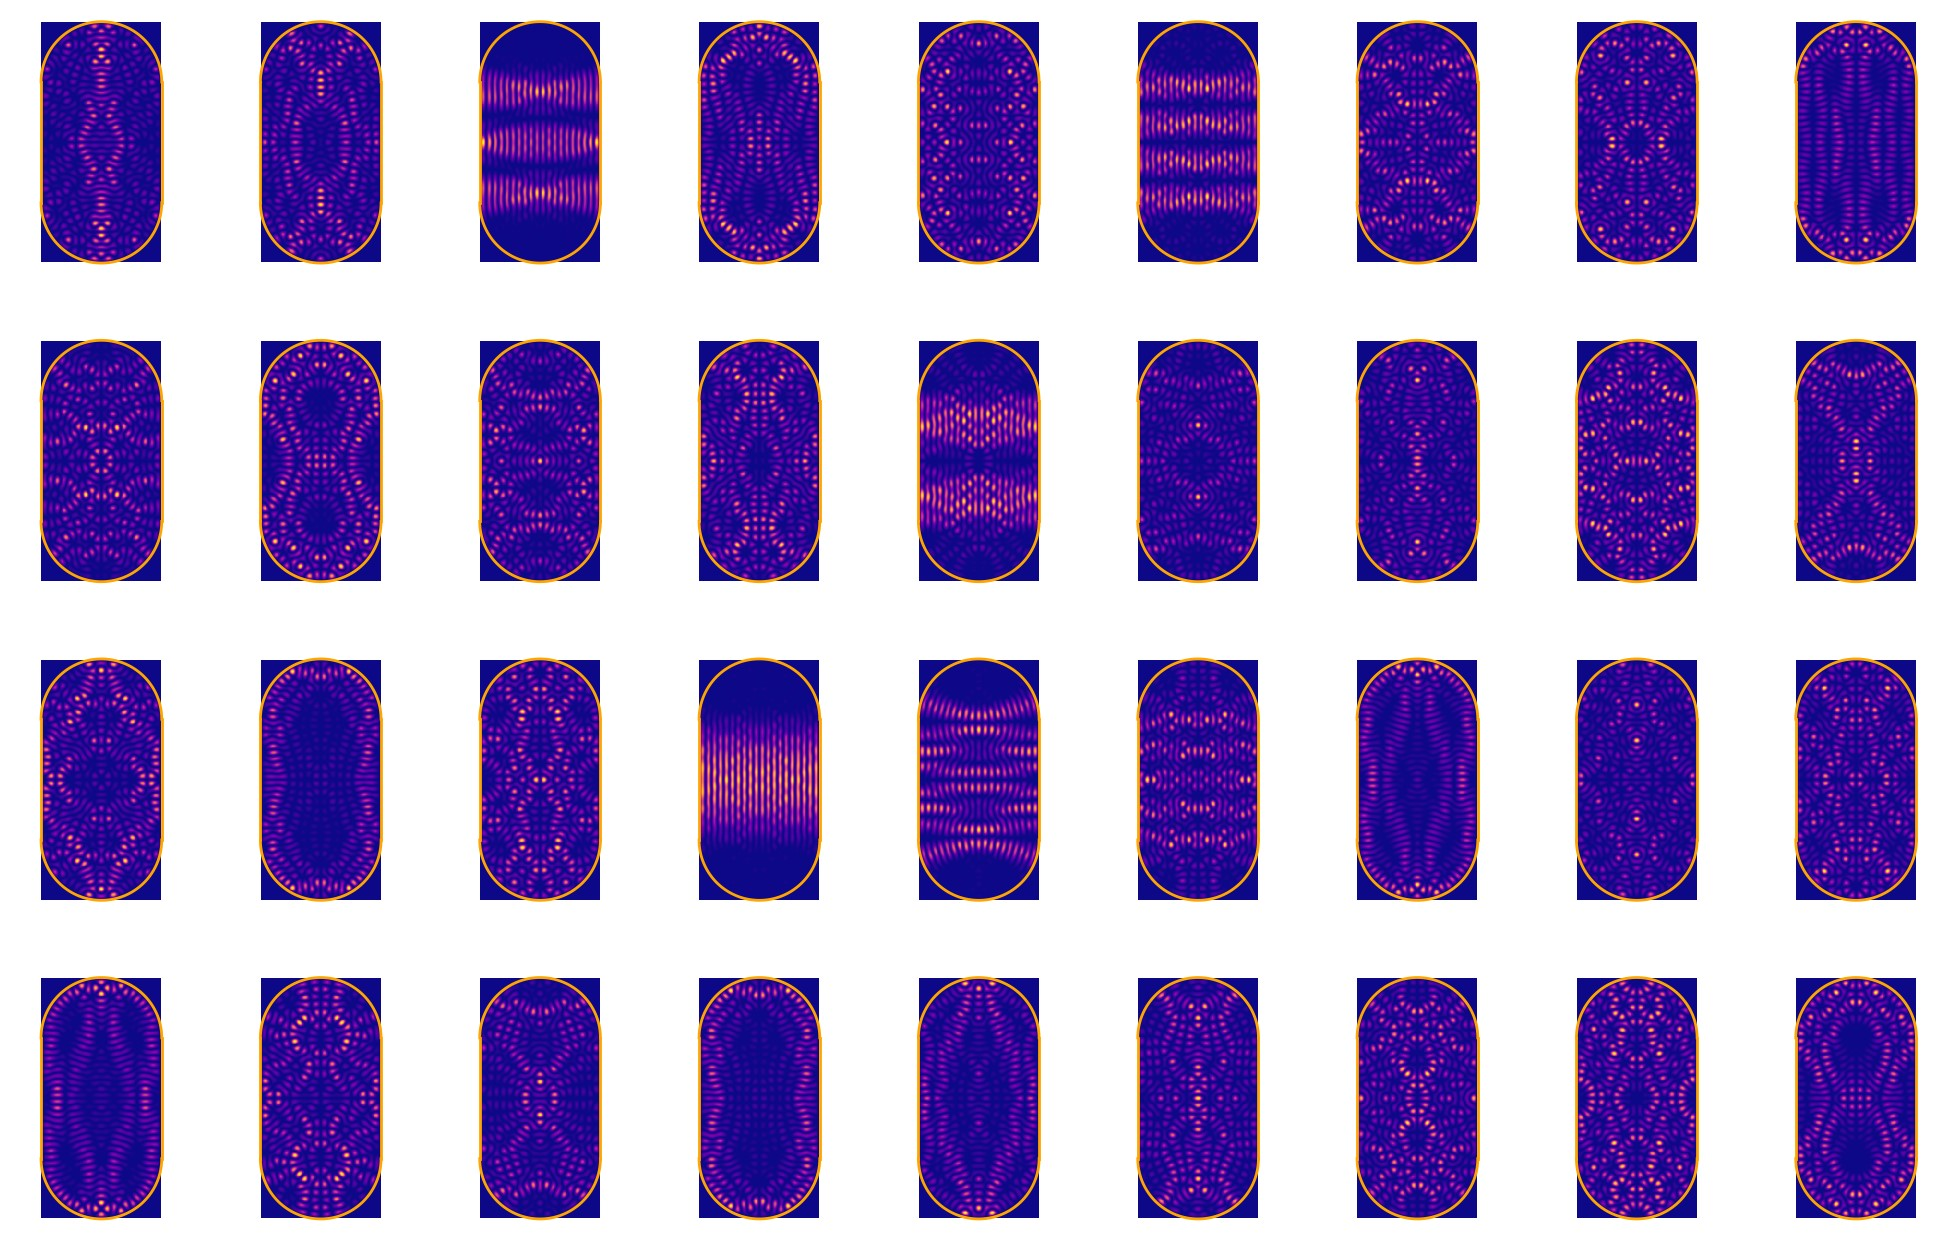
\includegraphics[scale=0.32,angle=0]{quant_stad_neig36_level1000_4per9.jpg}

    \noindent\\
  \decoRule
  \caption{Bunimovich stadium 36 eigenfunctions, for $\lambda\sim1000$}
  \label{fig:bunimov_eigenstates}
\end{figure}

 In fact, Hassell's main result (\cite{Hass:billiards_not}) shows that some high-eigenvalue eigenstates of $\BS_{l}$ do indeed have a positive mass on the bouncing ball orbits.

\begin{impTeo}{Hassell}{hassell_stadium}
For every $\veps>0$, there exist a subset $B_{\veps}\subset[1,2]$ of measure at least $1-4\veps$ and a constant $m(\veps)>0$ with the following property: for every $l\in B_{\veps}$, there exist a quantum limit formed from Dirichlet eigenfunctions of $\Lapl$ on the $\BS_{l}$ that gives probability mass at least $m(\veps)$ to the bouncing ball trajectories.
\end{impTeo}


The result of Hassell was foreshadow by numerical computations (see also chapter \ref{Chapter6}) and is based on construction of \emph{quasi-modes}, approximate solutions for
eigenfuctions given by Wentzel-Kramers-Brillouin (WKB) methods. The main obstacle in reaching the proof was to show that \virg{bouncing-ball} eigenfunctions (i.e. the corrispondent wigner measures) exist in the high-energy limit. Hassell's proof is a combination of the following techniques:


\begin{compactitem}
\item the \emph{Heller-Zelditch argument}, mettere referenza:\\ 
this method shows that eigenfunctions of $\Lapl$ localize on any Bunimovich stadium $\BS_{t}$, with the (possible) exception of eigenvalues lying in intervals of the form $[n^{2}-O(1),n^{2}+O(1)]$, with $n\in\N$. It can be proved that, if there really only $O(1)$ eigenvalues in this intervall, then eigenfunctions can localize, i.e. \virg{scarring} can occur in momentum space for these intervals (see Tao \cite{tao:site}). Reaching this bound ($O(1)$) is the difficult part of this step; 
\item the \emph{Hadamard variation formula}:\\
one of the main difficulties in approaching the previous task is the fact that Weyl's law has too large error term to get the desired bound. Hassell used this formula, which shows how the eigenvalues of $\BS_{l}$ vary with the aspect ratio of its rectangular component $t$. The formula is given by
\[
\frac{\dd }{\dd l}\lambda_{k}(l)=-\int_{\partial\BS_{l}}\frac{\sgn(x)}{2}(Y\cdot\overrightarrow{n})\abs{\partial_{\overrightarrow{n}}\vphi_{k}(x,l)}^{2}\dd s,
\]
where $(\vphi_{k},\lambda_{k})$ is an eigenvector-eigenvalue pair of the Laplacian $\Lapl$ with Dirichlet boundary condition on $\BS_{l}$, $\overrightarrow{n}$ is the outward unit normal vector at $\partial\BS_{l}$ and $\dd s$ is \virg{curvilinear element} on $\partial\BS_{t}$. Since $\sgn(x)/2(\partial_{x}\cdot\overrightarrow{n})\geq0$ always, the formula shows that, as $t$ increases, the magnitude of $\lambda_{k}$ decreases instead, for fixed $k$. One should not be surprised by this, because Weyl's law gives us 
\[
\lambda_{k}=\frac{4\pi k}{\Area(\BS_{t})}(1+o(1))
\]
and we see that $t$ and $\lambda_{k}$ are \virg{almost inversely proportional}. Using this formula, Hassell shows the refinement
\[
-\frac{\dd}{\dd l}\lambda_{k}(l)\sim \lambda_{k}(l)
\]
in expectation over $k$.
\item \emph{quantum unique ergodicity}:\\
this is used to reach a contradiction. More explicity, if $\BS_{l}$ is \QUE, then by Egorov's theorem \ref{impTeo:egorov} essentially positions and momenta of eigenfunctions in $T^{\ast}\BS_{l}$ are driven by the geodesic flow. At this point, Hassell uses this general argument (\cite{tao:site},\cite{Hass:billiards_not}): in classical dynamics, all geodesic in $\BS_{t}$ eventually interesect its boundary, and it can be shown that for any equidistributed eigenfunction, its normal derivative is also equidistributed on $\partial\BS_{l}$; hence, all eigenfunctions are equidistributed on $\partial\BS_{l}$ and this would imply that the exponential decay, given by Hadamard formula, holds for every $\lambda_{k}$, and not just in expectation. If this would be the case, it could be shown besides that the $\Lapl$-eigenvalues cannot concentrate in interval of the form $[n^{2}-O(1),n^{2}+O(1)]$ for most $l\in [1,2]$, else the eigenvalues would lay around $n^{2}$ for intervals of $t$ of measure non-zero, getting a contradiction with the exponential decay. The Heller-Zelditch argument then gives a contradiction to \QUE assumption.
\end{compactitem}


\begin{remark}
\label{remark:unique_non_que_bun_std}
It is important to highlight that the Bunimovich Stadium $\BS_{l}$ is the only known dynamical billiard for which we have a complete understanding of \QE and \QUE to date. In particular, it is the only one for which we know that \QUE does not hold. On the contrary, there many other systems, like the cardioid stadium $\CS$ and Barnett stadium are believed to be \QUE.
\end{remark}


METTERE FIGURA CARDIOIDE AUTOFUNZIONI?


%\subsection{Quantum maps}
%
%Cita MARKLOFF
%
%It is oftentimes useful to extend the ergodicity of the geodesic flow to the ergodicity of any map on the sympletic phase space $T^{\ast}M$, where $(M,g)$ is a Riemannian manifold. The dynamics on this system can be provided by a discrete map 
%
%
%An explicit and one of the most famous example of this subject is given by \emph{Arnold's cat map}, defined by the action of the map
%\[
%\Sigma=\Matrix{1&1\\1&2}
%\]
%on the 2-dimensional torus $\T^{2}$. In coordinates, for $(q,p)\in \R^{2}\setminus\Z^{2}$, we have $(x,y)\mapsto(q+p,q+2p)\mod1$. Without going in details, altough it has been shown that analogue of \QUE for hyperbolic toral automorphisms (properly speaking, symplectomorphisms) fails to hold (this does not contradicts remark \ref{remark:unique_non_que_bun_std}, as this system is not related to billiards). This suggests that may be something unique about the geodesic flow on a negatively curved manifold. 



%METTI FIGURA AZIONE MAPPA ARNOLD



% Chapter Template

\chapter{Seldberg trace formula} % Main chapter title

\label{Chapter4} % Change X to a consecutive number; for referencing this chapter elsewhere, use \ref{ChapterX}
\thispagestyle{empty}
%----------------------------------------------------------------------------------------
%	SECTION 1
%----------------------------------------------------------------------------------------

Trace formulas, in general, establish a connection between geometrical quantities with the spectra of a differential operator. Thus, they have the following form
\[
\sum\left\{
\text{spectral terms}
\right\}
=
\sum\left\{
\text{geometrical terms}
\right\}.
\]
We will now consider an introductive example, taken from \cite{Markloff:article}, to introduce this subject.

\section{Trace formula on $\S^{1}$}


\label{sec:intro_trace_for_s1}
A first example of a trace formula can be derived from the famous \emph{Poisson summation formula}

\begin{equation}
\label{eq:poisson_summation_formula}
\sum_{m\in\Z}h(m)=\sum_{n\in\Z}\int_{\R}h(t)\e^{2\pi\imi nt}\dd t=\sum_{n\in\Z}\Four{h}(n)
\end{equation}
which holds for $h\colon\R\to\mathbb{C}$ of class $C^{2}$ and such that $\abs{h(t)}$ is of \virg{rapid decay} (as in the Schwarz space $\schwarz$). Usually, it is used to derived the functional equation of Riemann's zeta function. We can now read this formula as a \emph{trace formula}.\\

Consider the Laplacian $-\Lapl$ on the unit circle $\S^{1}$. This ammounts on studying the equation
\[
-\Lapl u=\lambda u,\; u(0)=u(2\pi)
\]
which has solutions of the form $\vphi_{n}(x)=(2\pi)^{-1/2}\e^{\imi nx}$ with $\lambda=n^{2}$. Considering the linear operator $L$ acting on $2\pi$-periodic functions and defined by
\[
[Lf](x)\coloneqq \int_{0}^{2\pi}k(x,y)f(y)\dd y
\]
where the integral kernel $k(x,y)$ is given by
\[
k(x,y)=\sum_{m\in\Z}h(m)\vphi_{m}(x)\overline{\vphi}_{m}(y).
\]
Then, due to the orthogonality in $L^{2}([0,2\pi])$ of eigenfunctions $\vphi_{n}(x)$, we have 
\[
L\vphi_{n}=h(n)\vphi_{n}
\]
and hence the left hand side of equation \eqref{eq:poisson_summation_formula} can be read as a \virg{spectral sum} over eigenvalues. In particular, it holds
\[
\tr L=\sum_{n\in\Z}\int_{\R}h(t)\e^{2\pi\imi nt}\dd t.
\]
The right hand is of this last equation has an immediate geometric interpretation, as sum over all geodesics (in $S^{1}$) of length $2\abs{n}$.\\
Now, we choose the function $h(t)=(\lambda^{2}-t^{2})^{-1}$, which appears dealing with the resolvent operator of the Laplacian $(\Lapl+\lambda^{2})$. For further details we refer to \cite{Markloff:article}. Poisson summation formula gives
\[
\sum_{m\in\Z}\frac{1}{\lambda^{2}-m^{2}}=\sum_{n\in\Z}\int_{\R}\frac{\e^{2\pi\imi nt}}{\lambda^{2}-t^{2}}\dd t.
\]
The integral term can be rewritten as follows. If $n$ is non-positive, then 
\[
\int_{\R}\frac{\e^{2\pi\imi nt}}{\lambda^{2}-t^{2}}\dd t=\int_{\R}\frac{\e^{-2\pi\imi\abs{n}t}}{\lambda^{2}-t^{2}}\dd t
\]
while in the other case, with the substitution $t\mapsto-t$,
\[
\int_{\R}-\frac{\e^{-2\pi\imi nt}}{\lambda^{2}-(-t)^{2}}\dd t=\int_{\R}\frac{\e^{-2\pi\imi\abs{n}t}}{\lambda^{2}-t^{2}}\dd t
\]
In conclusion, 
\[
\sum_{m\in\Z}\frac{1}{\lambda^{2}-m^{2}}=\int_{\R}\frac{\e^{-2\pi\imi\abs{n}t}}{\lambda^{2}-t^{2}}\dd t
\]
Considering the rectangle 
\[
\gamma = \{t\}\cup\{M+\imi(t+M)\}\cup\{-t+2M\imi\}\cup\{-M+\imi(M-t)\} = \gamma_{1}\cup\gamma_{2}\cup\gamma_{3}\cup\gamma_{4},\quad \forall t\in[-M,M]
\]
with $M>0$ and using the Residue Theorem to compute the integral of $f(t)=\frac{\e^{-2\pi\imi\abs{n}t}}{\lambda^{2}-t^{2}}$ along $\gamma$ (clockwise) we get
\[
\int_{[-M,M]}\frac{\e^{-2\pi\imi\abs{n}t}}{\lambda^{2}-t^{2}}\dd t=\int_{\gamma_{2}\cup\gamma_{3}\cup\gamma_{4}}\frac{\e^{-2\pi\imi\abs{n}z}}{\lambda^{2}-t^{2}}\dd z+2\pi\imi\Res(f,\lambda).
\]
It can be shown with simple standard bounding techniques that the integral over the complex segments $\gamma_{2}\cup\gamma_{3}\cup\gamma_{4}$ vanishes for $M\to\infty$. Hence we get 
\[
\int_{\R}\frac{\e^{-2\pi\imi\abs{n}t}}{\lambda^{2}-t^{2}}\dd t=2\pi\imi\Res(f,\lambda)=2\pi\imi\frac{\e^{-2\pi\imi\abs{n}\lambda}}{2\lambda}=\frac{\pi\imi}{\lambda}\e^{-2\pi\imi\abs{n}\lambda}.
\]
So,
\[
\sum_{m\in\Z}\frac{1}{\lambda^{2}-m^{2}}=\frac{\pi\imi}{\lambda}\sum_{n\in\Z}\e^{-2\pi\imi\abs{n}\lambda}.
\]
The right hand side is linked to $\cot z$ function on the half plane $\Im(z)<0$, as
\[
\cot z=\frac{\cos z}{\sin z}=\imi\frac{1+\e^{-2\imi z}}{1-\e^{-2\imi z}}=\imi(1+\e^{-2\imi z})\sum_{n=0}^{\infty}\e^{-2\imi n z}=\imi\sum_{n\in\Z}\e^{-2\imi\abs{z}}.
\]
In the end it is proved 
\[
\sum_{m\in\Z}\frac{1}{\lambda^{2}-m^{2}}=\frac{\pi}{\lambda}\cot(\pi\lambda)
\]
We will now go deeper in trace formula for hyperbolic surfaces, regarding Laplacian eigenfunctions. This form resembles the general structure of a trace formula, where often trigonometric and hyperbolic functions are present. In the general case for $h$ the final formula is the following. 

\begin{nteo}
Let $h\colon\mathbb{C}\to\mathbb{C}$ a function which is analytic for $\abs{\Im(z)}\leq \sigma$, for a certain $\sigma>0$. Moreover, suppose that $h(z)$ is such that
\[
\abs{h(z)}\ll(1+\abs{\Re(z)})^{-1-\delta}
\]
for some $\delta>0$, uniformly for all $z$ in the strip $\abs{\Im z}\leq \sigma$.
\end{nteo}

Its proof follows verbatim the previous reasonings. 


\section{Laplacian operator}

Driven by the previous example, we now approach the Seldeberg trace formula for the case of interest. In this situation, as foretold before, our differential operator will be the Laplacian. On the main reasons for the importance of Laplace-Beltrami operator (for brevity, Laplace or Laplacian) is that it's the unique (up to scalar multiplication) second order differential operator that commutes with actions of the isometry group.\\
Thinking about homogeneity and isotropy in physics, this can help explaining its widespread presence in most of partial differential equations (Schr{\"o}dinger equation, wave equation ecc.)
At first, in this chapter, we will introduce main properties of Laplacian on hyperbolic surfaces and will develop, without going in details however, notions of harmonic analysis for this context. The final aim will be to explore the connection between eigen-spectrum of the Laplacian and the dynamical properties of hyperbolic surfaces, namely the Seldberg trace formula.

Explicity, the Laplace operator on a Riemannian manifold with metric $g$ is given in local coordinate by
\[
\Lapl f = \frac{1}{\sqrt{\abs{g}}}\partial_{i}\left(\sqrt{\abs{\Hmetr}}\Hmetr^{ij}\partial_{j}f\right)
\]
where $\abs{\Hmetr}$ is the determinant of metric tensor $\Hmetr$ and $\Hmetr^{ij}$ are the components of inverse metric tensor $\Hmetr^{-1}$. In the euclidian case we get the usual Laplacian, but in the hyperbolic case (upper-half plane model $\Hilb$)
\[
\Hmetr_{ij}=\frac{\delta_{ij}}{y^{2}}
\]
In this case, $\Hmetr^{ij}=y^{2}\delta^{ij}$ and $\sqrt{\abs{\Hmetr}}=y^{-2}$. Then with easy computations,
\[
\Lapl f=y^{2}(\partial_{xx}f+\partial_{yy}f).
\]
The Laplacian can be seen as a differential operator on any hyperbolic surface $M=\Gamma\setminus\Hilb$. However, for simplicity, we will assume $M$ \underline{compact} and we fix a fundamental domain $D$ for $M$. In this sense, any $f\colon D\to\mathbb{C}$ can be seen as a $\Gamma$-invariant function on $\Hilb$ and its integral over $D$ is given by $\int_{D}f\dd\mu$.

\begin{nlem}
If $A\in\PSL_{2}\R$ and $T_{A}(f)=f(A^{-1}z)$ for $f\in C^{\infty}(\Hilb)$, then 
\[
\Lapl T_{A}=T_{A}\Lapl.
\]
\end{nlem}
\begin{prf}
It's sufficient to check the property in case $A=\SmallQmatrix{0&-1\\1&0}$ or $A=\SmallQmatrix{1&x\\0&1}$, for some $x\in\R$, as these two matrices generates all $\PSL_{2}\R$.
\end{prf}

\begin{remark}
Very often, it's considered as the Laplacian the operator $-\Delta$, because in this way the eigenvalues are positive, see the following result.
\end{remark}

\begin{nteo}
\label{teo:spectra_laplace}
There exists a sequence $\{\vphi_{j}\}_{j\in\N}$ of $L^{2}(M)$ of Laplacian-eigenfunctions
\[
\Delta\vphi_{j}=\lambda_{j}\vphi_{j}
\]
with corrisponding (positive) eigenvalues $\lambda_{j}$ such that $\{\lambda_{j}\}_{j}$ is a increasing and diverging sequence of positive real numbers and $\{\vphi_{j}\}_{j\in\N}$ form a orthonormal basis of $L^{2}(M)$.
\end{nteo}
\begin{prf}
See \cite{Masson:aque_everything}.
\end{prf}

The proof of this theorem is based on the use of spectral decomposition theorem for compact operators. However, as the Laplacian is not compact, it is necessary to use some approximating compact operators (\emph{heat kernel}), showing that the share the same spectrum of the Laplacian. Here are some general properties for the Laplacian.

\begin{nprop}
The followings hold.
\begin{compactitem}
\item $\Lapl$ is a symmetric operator, i.e. $\pscl{\Lapl f}{g}=\pscl{f}{\Lapl g}$ for any $f,g\in C^{\infty}(M)$.
\item If $f\in C^{\infty}(M)$ is not constant, then $\pscl{\Lapl f}{f}$ is positive.
\end{compactitem}
\end{nprop}



\subsection{A brief journey across harmonic analysis on the hyperbolic plane}

\label{subsec:harmonic_analysis_hyperbolic}


To prove, in the subsequent sections, the Seldberg trace formula, we will now some notions taken from the field of harmonical analysis (see \cite{Evans:book},\cite{Horm:book1})\\

DA FINIRE IL DISCORSO\\

The starting point is the definition of the \emph{invariant kernel}.

\begin{defin}
\label{def:invariant_kernel}
An invariant kernel is a function $\kernel\colon\Hilb\times\Hilb\to\mathbb{C}$ with the following characteristics:
\begin{compactenum}
\item $\kernel(\gamma z,\gamma w)=\kernel(z,w)$ for all $\gamma\in\Isom(\Hilb)=\PSL_{2}\R$ and for all $(z,w)\in\Hilb\times\Hilb$;
\item $\kernel(\cdot,\cdot)$ is symmetric in its arguments.
\end{compactenum}
\end{defin}

Such a kernel carries with it an \emph{invariant integral operator} $I$ defined by
\[
If(z)=\int_{\Hilb}\kernel(z,w)f(w)\dd\mu(w).
\]
with $f$ that must satisfy appropriate conditions. This induces an operator on the quotient surface $M=\Gamma\setminus\Hilb$, in particular for $f$ $\Gamma$-invariant:
\[
If(z)=\sum_{\gamma\in\Gamma}\int_{D}\kernel(z,\gamma w)f(w)\dd\mu(w).
\]
with $D$ fundamental domain for $\Gamma$.\\
We will consider invariant kernels of the form 
\[
\kernel(d(z,w))
\]
where $\kernel\colon\R\to\mathbb{C}$ is an even function. With abuse of notation, we will use $\kernel(z,w)$ for complex $z,w$ or $\kernel(l)$ for real $l$ indifferently, instead of $\kernel(d(z,w))$.

\begin{nprop}
\label{prop:eig_Lapl_is_eig_operator}
If $f$ is an eigenfunction of the Laplacian of eigenvalue $\lambda$, then it is also an eigenfunction of the invariant integral operator $I_{\kernel}$ relative to $\kernel$. Hence, there exists a function $h\colon\R\to\mathbb{C}$ such that 
\[
I_{\kernel}f(z)=\int\kernel(d(z,w))f(w)\dd\mu(w)=h(\lambda)f(z).
\]
\end{nprop}
\begin{prf}
Let $f$ be an eigenfunction of the Laplacian of eigenvalue $\lambda$. We define the corrisponding radial function 
\[
F_{z}(w)=\int_{S_{z}}f(Mw)\dd M
\]
where $S_{z}=\Stab_{z}$ and $\dd M$ is the normalised Haar measure on $S_{z}$. It is a radial eigenfunction and, by the subsequent lemma \ref{lem:techincal} we know that
\[
F_{z}(w)=\vphi_{\lambda}(z,w)f(z).
\]
So we have
\begin{align*}
\int_{\Hilb}\kernel(z,w)f(w)\dd\mu(w)&=\int_{S_{z}}\int_{\Hilb}\kernel(z,M^{-1}w)f(w)\dd\mu(w)\dd M\\
&=\int_{S_{z}}\int_{\Hilb}\kernel(z,w)f(Mw)\dd\mu(w)\dd M\\
&=\int_{\Hilb}\kernel(z,w)F_{z}(w)\dd\mu(w).
\end{align*}
Hence
\[
\int_{\Hilb}\kernel(z,w)f(w)\dd\mu(w)=h(\lambda)f(z),
\]
where the \virg{eigenvalue} $h(\lambda)$ is given by
\[
h(\lambda)=\int_{\Hilb}\kernel(z,w)\vphi_{\lambda}(z,w)\dd\mu(w).
\]
What remains to be proved is that $h(\lambda)$ is indipendent of $z$ and for any $g\in\PSL_{2}\R$:
\begin{align*}
\int_{\Hilb}(gz,w)\vphi_{\lambda}(gz,w)\dd\mu(w)&=\int_{\Hilb}\kernel(z,g^{-1}w)\vphi_{\lambda}(z,g^{-1}w)\dd\mu(w)=\\
&=\int_{\Hilb}\kernel(z,w)\vphi_{\lambda}(z,w)\dd\mu(w).
\end{align*}
This concludes the proof.
\end{prf}


\begin{nlem}
\label{lem:techincal}
For any $\lambda\in\mathbb{C}$ and $z$ in the upper-half plane, there exists a unique function $w\mapsto\vphi_{\lambda}(z,w)$, with radial symmetry centered in $z$, such that
\begin{compactenum}
\item $\vphi_{\lambda}(z,z)=1$;
\item $\Lapl_{\Hmetr}\vphi_{\lambda}(z,w)=\lambda\vphi_{\lambda}(z,w)$.
\end{compactenum} 
\end{nlem}
\begin{prf}
Omitted (\cite{Masson:aque_everything}).
\end{prf}

We define the Seldberg transform $\SelT(k)$ of a radiant kernel $\kernel$ as %pg25 from basics to aque...
\begin{equation}
\label{eq:def_seldberg_transform}
\SelT(\kernel)(\lambda)=h(\lambda)=\int_{\Hilb}\kernel(d(\imi,w))\vphi_{\lambda}(\imi,w)\dd\mu(w).
\end{equation}
We will use the re-parametrisation $\lambda=s(1-s)=1/4+r^{2}$, with $r\in\mathbb{C}$ we will write indifferently, with abuse of notation, $\SelT(\kernel)(r)$ and $\SelT(\kernel)(\lambda)$.

\begin{nprop}
\label{prop:seld_transform_formula}
The Seldberg transform $\SelT(\kernel)$ of a radian kernel $\kernel$ can be computed with the Fourier transform of the function
\[
g(u)=\frac{1}{\sqrt{2}}\int_{\abs{u}}^{\infty}\frac{\kernel(\rho)\sinh\rho}{\sqrt{\cosh\rho-\cosh u}}\dd\rho
\]
so that 
\[
\SelT(\kernel)(r)=\Fourier(g)(x).
\]
\end{nprop}
\begin{prf}
Let $f\colon\mathbb{C}\to\mathbb{C}$ defined by $f(z)=y^{1/2+\imi r}$, for $z=x+\imi y$ and fixed $r$. We have that
\[
-\Lapl_{\Hmetr}f(z)=y^{2}\cdot\left((1/4+ r^{2}) y^{1/2-2+\imi r}\right)=f(z)
\]
so it is an eigenfunction of the Laplacian with eigenvalue
\[
\lambda=\frac{1}{4}+r^{2}=s(1-s)
\]
for a certain $s\in\mathbb{C}$. With abuse of notation, we will write $h(r)=h(\lambda)$, instead of $h(\lambda(r))$. By proposition \ref{prop:eig_Lapl_is_eig_operator}, we have that
\[
h(r)=\int\kernel(d(\imi,z))\Im(z)^{1/2+\imi r}.
\]
Let $U(\cosh\rho)=\kernel(\rho)$ so that, using formula for hyperbolic distance
\[
U\left(
1+\frac{\abs{z-w}^{2}}{2\Im(z)\Im(w)}
\right)=\kernel(d(z,w)).
\]
Hence we have 
\[
h(r)=\int_{-\infty}^{\infty}\int_{0}^{\infty}U\left(
\frac{1+x^{2}+y^{2}}{2y}
\right)y^{1/2+\imi r}\frac{\dd y}{y^{2}}\dd x.
\]
Letting $\cosh\rho=(1+x^{2}+y^{2})/2y$ (substitution with respect to variable $x$) and $y=\e^{u}$, we have
\[
x=\pm\sqrt{2\e^{u}\cosh\rho-1-\e^{2u}},\quad \sinh\rho\dd\rho=\frac{x}{y}\dd x,\quad \e^{u}\dd u=\dd y
\]
and then\footnote{The minimum value of $\cosh\rho$ is $\frac{1+\e^{2u}}{2\e^{u}}=\cosh u$ and so $\rho\geq\abs{u}$.}
\[
h(r)=\int_{-\infty}^{\infty}\int_{\abs{u}}^{\infty}\frac{U(\cosh\rho)}{\e^{2u}}\cdot\left(\e^{u}\right)^{1/2+\imi r}\cdot\frac{y\sinh\rho}{x} \e^{u}\dd \rho\dd u=\frac{1}{\sqrt{2}}\int_{-\infty}^{\infty}\int_{\abs{u}}^{\infty}\frac{\kernel(\rho)\sinh\rho}{\sqrt{\cosh\rho-\cosh u}}\cdot \e^{\imi r}\dd \rho\dd u.
\]
The result is proved.
\end{prf}

It can be also shown that it is possible to revert the Seldberg transform also using Fourier inversion formula, with a different \virg{weight function}.

\begin{nprop}
\label{prop:inverse_seld_transform}
For a function $h\colon\R\to\mathbb{C}$, the Seldberg transform is inverted using the inverse Fourier transform
\[
g(u)=\frac{1}{2\pi}\int_{-\infty}^{\infty}\e^{-\imi ru}h(r)\dd r
\]
with 
\[
\kernel(\rho)=-\frac{1}{\sqrt{2}\pi}\int_{\rho}^{\infty}\frac{g'(u)}{\sqrt{\cosh u-\cosh\rho}}\dd u.
\]
\end{nprop}
\begin{prf}
Omitted.
\end{prf}


\section{Periodic geodesics}

\label{sec:period_geodesics}


The trace formula is a bridge between spectral property of a system, namely the spectrum of the Laplacian, and its geometrical charateristics, i.e. the set of lengths of closed geodesics.\\
Let $M=\Gamma\setminus\Hilb$ be a \underline{compact hyperbolic surface}, so that $\Gamma$ does not contain any parabolic element. We further assume that $M$ can be considered as a regular Riemann surface, hence $\Gamma$ has not elliptic elements either.\\
The spectrum of the Laplacian is denoted by 
\[
\lambda_{j}=\frac{1}{4}+\rho_{j}^{2}
\]
and, as $\lambda_{j}\in\R$, we have that $\abs{\Im(\rho_{j})}\leq1/2$.


\begin{defin}
\label{def:closed_geod}
A \emph{periodic} or \emph{closed geodesic} in $M$ is a geodesic $\gamma\colon\R\to M $ such that $\exists T>0$
\[
(\gamma(t+T),\gamma'(t+T))=(\gamma(t),\gamma'(t)),\;\forall t\in\R.
\] 
The set of closed geodesic in $M$ will be denoted by $\ClsdGeod{M}$. The smallest $T>0$ for which this is true, is denoted by $\ell(\gamma)$ and it's called the \emph{period or length} of the geodesic $\gamma$. 
\end{defin}

As we said in section METTI SEZIONE, for every hyperbolic element $A\in\Gamma$, there is one and only geodesic invariant with respect to the action of $A$, namely the \emph{axis} of $A$, see \eqref{eq:invar_geodes_hyperb}. It's possible to prove the following result.



\begin{nlem}
% konstantine
If $M=\Gamma\setminus\Hilb$ is an hyperbolic compact surface, then for every hyperbolic element $g\in\Gamma$ the projection of the axis $\gamma$ of $g$ in $M$ is a closed geodesic of length $\ell_{g}$.
\end{nlem} 
\begin{prf}
CITA KONSTANTINE
\end{prf}

It's interesting to see how the length $\ell_{g}$ is linked to the matrix $g$. If 
\[
g=\Qmatrix{
a&b\\c&d
}
\]
then this matrix it's similar to 
\[
A_{\ell}=\Qmatrix{\exp(\ell/2)&\\&\exp(-\ell/2)}
\]
for a certain $\ell>0$. We have that $d(z,Az)=\ell$ and hence this is still true for $g$, so $\ell$ it's exactly the length of the axis of $g$. In particular we have that
\[
2\cosh\ell=\abs{\tr g}.
\]
This relation can be restated with eigenvalues of $g$: if $1<\lambda$ and $\lambda^{-1}$ are $g$'s eigenvalues, than this equation rewrites as
\[
\ell_{g}=\log\lambda^{2}.
\]

\begin{defin}
\label{def:prim_elem}
An element $\gamma\in\Gamma$ is called \emph{primitive} iff it cannot be expressed in the form $\delta^{k}$, with $k\geq2$ and $\delta$ is another elemento of $\Gamma$.  
\end{defin}

\begin{nprop}
\label{prop:hyp_elements_classes}
The set $\ClsdGeod{M}$ can be identified with the set of conjugacy classes in $\Gamma$ of primitive hyperbolic elements.
\end{nprop}
\begin{prf}
Let $\rho\in\ClsdGeod{M}$ and let $C_{\rho}$ be the class of geodesics of $\Hilb$ that project on $\rho$. Let $\gamma$ be a representative of this class. The stabilizer $\Stab_{\gamma}$ of $\gamma$ in $\PSL_{2}\R$ is the set of hyperbolic transformations fixing $\gamma$. It is conjugate to the diagonal subgroup (see METTI REFERENZA)
\[
\left\{
\Qmatrix{\exp(t/2)&\\&\exp(-t/2)},\; t\in\R
\right\}.
\]
In particular $\Stab_{\gamma}\simeq\R$. Hence, the subgroup $\Stab_{\gamma}\cap\Gamma$ is homomorphic to a discrete subgroup of $\R$, being $\Gamma$ a discrete subgroup, and so it's cyclic. Let $\delta\in\Gamma$ such that 
\[
\Stab_{\gamma}\cap\Gamma=\spn{\delta}.
\]
Obviously, $\delta$ must be primitive. Any other representative $\hat{\gamma}$ of $C_{\rho}$ is obtained as $\hat{\gamma}=g\gamma$, with $g\in\Gamma$, and so 
\[
\Stab_{\hat{\gamma}}\cap\Gamma=\spn{g\delta g^{-1}}.
\]
Let $C_{\delta}$ be the conjugacy class of $\delta$ in $\Gamma$. Then, we have built a map $\rho\mapsto(C_{\gamma}\mapsto C_{\delta})$ associating a conjugacy class in $\Gamma$ of primitive hyperbolic elements to a periodic geodesic, which is one-to-one.
\end{prf}

At this point, we can establish the approximate growth for the number of closed geodesic (not necessary primitive) with length at most $L$.

\begin{nprop}
\label{prop:numb_geod_growth}
Let $X=\Gamma\setminus\Hilb$ be an hyperbolic compact surface. Then the number of closed geodesics $c_{X}(L)$ on $X$ with length at most $L$ is $O(\e^{L})$.
\end{nprop}
\begin{prf}
Let $x\in X$ be a point on the surface and let $w$ be the corrispondent point on $\Hilb$, so that $\pi(w)=x$. Let $D_{w}$ be the Dirichlet domain of center $w$ for $\Gamma$. If $\gamma$  is a closed geodesic on $X$ of length at most $L$, then let $\gamma'$ be its lifting on $\Hilb$, passing through a point $q\in D_{w}$. This curve $\gamma'$ is a geodesic on $\Hilb$ and it is fixed (as geodesic) by an hyperbolic element $G\in\Gamma$. Let $d$ be the diameter of the domain $D_{w}$, which is finite as $X$ is compact. Then we get
\[
d(w,Gw)\leq d(w,q)+d(q,Gq)+d(Gq,Gw)\leq L+2d.
\] 
Hence, for each geodesic of length at most $L$, there exist an element $G\in\Gamma$ such that $w$ is sent inside a (hyperbolic) ball of center $w$ and ray $L+2d$. Hence, $c_{X}(L)$ is bounded by the number of images of the domain $D_{w}$ which are distant at most $L+2d+d$ from $w$. For $L$ \virg{big enough}, thus the following estimate hold
\[
c_{X}(L)\simeq\frac{\mu_{\Hilb}(B(w,L+3d))}{\mu_{\Hilb}(D_{w})}.
\]
Using the Poincaré disk model, a hyperbolic ball of hyperbolic radius of $R=L+3d$, centered in $0$, can be seen as an Euclidian disk with radius $\tanh(R/2)$. Thus, the area is given by
\begin{align*}
\mu_{\Hilb}(B(w,R))&=\mu_{\Disk}(B(0,R))=\iint_{B(0,R)}\frac{4}{(1-\abs{z}^{2})}\dd x\dd y\stackrel{z=r^{e^{\imi\theta}}}{=}\int_{0}^{2\pi}\int_{0}^{\tanh(R/2)}\frac{4r}{(1-r^{2})^{2}}\dd r\dd \theta\\
&=4\pi\left[\frac{1}{1-r^{2}}\right]_{0}^{\tanh(R/2)}=4\pi\cosh^{2}(R/2)
\end{align*}
and this gives what desired.
\end{prf}



\section{Pretrace formula}

The general form of Seldberg is the following: for any \virg{admissible function}\footnote{In the following will be more precise.} $h$,
\[
\sum_{j=0}^{\infty}h(r_{j})=\frac{\Area(M)}{4\pi}\int_{-\infty}^{+\infty}h(r) r \tanh(\pi r)\dd r+\sum_{\gamma\in} 
\]
where, as in the previous secion, $\mathcal{G}(M)$ the set of periodic geodesics of $M$. 


Let $\{\vphi_{j}\}_{j\in\N}$ be a orthonormal basis of (real) eigenfunctions of $\Delta$ on $L^{2}(M)$, as in theorem \ref{teo:spectra_laplace}.

\begin{nprop}
\label{prop:pretrace_formula}
Let $h$ be the Seldberg transform of radial kernel $\kernel$, we have
\[
\sum_{j=0}^{\infty}h(r_{j})\vphi_{j}(z)\vphi_{j}(w)=\sum_{\gamma\in\Gamma}\kernel(z,\gamma w),
\]
where the convergence is absolute and uniform. When $z=w$, we get 
\begin{equation}
\label{eq:pretrace}
\sum_{j=0}^{\infty}h(r_{j})\abs{\vphi_{j}(z)}^{2}=\frac{1}{4\pi}\int_{-\infty}^{\infty}h(x)\tanh(\pi x)x\dd x+\sum_{\gamma\in\Gamma\setminus\{e\}}\kernel(z,\gamma z).
\end{equation}
\end{nprop}
\begin{prf}
The eigenfunctions $\vphi_{j}$ are $\Gamma$-invariant functions on $\Hilb$, hence by definition of Seldberg transform we have
\[
\int_{\Hilb}\kernel(z,w)\vphi_{j}\vphi_{j}(w)\dd\mu(w) = h(r_{j})\vphi_{j}(z).
\]
At the same time 
\[
\int_{\Hilb}\kernel(z,w)\vphi_{j}(w)\dd\mu(w)=\int_{D}\sum_{\gamma\in\Gamma}k(z,\gamma w)\vphi_{j}(w)\dd\mu(w).
\]
The sequence $\{\vphi_{j}\}_{j\geq0}$ form a basis, so 
\[
\sum_{\gamma\in\Gamma}k(z,\gamma w)=\sum_{j\in\N}\left(
\int_{D}\sum_{\gamma\in\Gamma}k(z,\gamma z')\vphi_{j}(z')\dd\mu(z')
\right)\vphi_{j}(w)=
\sum_{j\in\N}h(r_{j})\vphi_{j}(z)\vphi_{j}(w),
\]
where the series converge in $L^{2}$. In \cite{Hejhal:seld_trace}, Hejhal proved that the series converge absolutely and uniformly in $z,w$.\\
To get \eqref{eq:pretrace}, we first prove that
\[
\kernel(z,z)=\frac{1}{4}\int_{-\infty}^{\infty}h(x)\tanh(\pi x)x\dd x.
\]
We start by writing the inverse Seldberg transform\footnote{See \ref{prop:inverse_seld_transform}}
\[
\kernel(z,z)=\kernel(d(z,z))=\kernel(0)=-\frac{1}{\pi\sqrt{2}}\int_{0}^{\infty}\frac{g'(u)}{\sqrt{\cosh u-1}}\dd u=-\frac{1}{2}\int_{0}^{\infty}\frac{g'(u)}{\sinh(u/2)}\dd u
\]
where $g(u)$ is the inverse Fourier transform
\[
g(u)=\frac{1}{2\pi}\int_{-\infty}^{\infty}h(r)\e^{-\imi u\rho}\dd\rho.
\]
Substituting and using Fubini theorem (thanks to rapid decay condition of $h$), we get 
\begin{align*}
\kernel(z,z)&=\frac{1}{4\pi^{2}}\int_{0}^{\infty}\int_{-\infty}^{\infty}h(\rho)\frac{\sin(u\rho)}{\sinh(u/2)}\rho\dd\rho\dd u\\
&=\frac{1}{4\pi^{2}}\int_{-\infty}^{\infty}h(\rho)\left(
\int_{0}^{\infty}\frac{\sin(u\rho)}{\sinh(u/2)}\dd u
\right)\rho\dd\rho.
\end{align*}
We now rewrite the term $1/\sinh(u/2)$ as a series
\[
\frac{1}{\sinh(u/2)}=\frac{2}{\e^{u/2}(1-\e^{-u})}=2\e^{-u/2}\sum_{n=0}^{\infty}\e^{-nu}
\]
and using its absolute convergence, we can interchange integration and summation
\begin{align*}
\int_{0}^{\infty}\frac{\sin(u\rho)}{\sinh(u/2)}\dd u&=2\sum_{n\geq0}\int_{0}^{\infty}\e^{-(2n+1)u/2}\sin(u\rho)\dd u\\
&=2\sum_{n\geq0}\frac{4\rho}{4\rho^{2}+(2n+1)^{2}}=\sum_{n\in\Z}\frac{4\rho}{4\rho^{2}+(2n+1)^{2}}.
\end{align*}
Moreover, we have the Fourier correspondence
\[
\int_{-\infty}^{\infty}\e^{-2\pi\imi x\zeta}\frac{2\rho}{\rho^{2}+\zeta^{2}}\dd\zeta= 2\pi \e^{-2\pi\rho\abs{x}}
\]
and we can use Poisson summation formula \eqref{eq:poisson_summation_formula}
\[
\sum_{n\in\Z}f(n)=\sum_{n\in\Z}\int_{-\infty}^{\infty}\e^{-2\pi\imi n\xi}f(\xi)\dd\xi
\]
finally getting
\[
\sum_{n\in\Z}\frac{\rho}{\rho^{2}+(n+1/2)^{2}}=
\pi\sum_{n\in\Z}\e^{\imi\pi n}\e^{-2\pi \rho\abs{n}}=\pi\frac{1-\e^{-2\pi \rho}}{1+\e^{-2\pi\rho}}=\pi\tanh(\pi \rho).
\]
To sum up, we have obtained that
\[
\int_{0}^{\infty}\frac{\sin(u\rho)}{\sinh(u/2)}\dd u=\pi\tanh(\pi\rho)
\]
and so the proof is complete.
\end{prf}

\begin{remark}
Even if Poisson summation formula could have appear to be a \virg{fictitious} tool to introduce Seldberg trace formula in section \ref{sec:intro_trace_for_s1}, in this proof one can see that these two subjects actually are linked together.
\end{remark}


To prove the complete version of Seldberg trace formula, it is necessary to integrate equation \eqref{eq:pretrace} over a fundamental domain $D$ (for example, a Dirichlet domain). We have 
\[
\sum_{j=0}^{\infty}h(r_{j})\abs{\vphi_{j}(z)}^{2}=\frac{\Area(M)}{4\pi}\int_{-\infty}^{\infty}h(x)\tanh(\pi x)x\dd x+\sum_{\gamma\in\Gamma\setminus\{e\}}\int_{D}\kernel(z,\gamma z)\dd\mu(z).
\]
We would like to rewrite the last term as a sum over closed geodesics. To this, we will group the terms by conjugacy classes $[\gamma]$, with $\gamma\in\Gamma$. If $\gamma_{0}\in [\gamma]$, then there exist a $g\in\Gamma$ such that $\gamma_{0}=g^{-1}\gamma g$. So
\begin{align*}
\int_{D}\kernel(z,\gamma_{0} z)\dd\mu(z)&=\int_{D}\kernel(z,g^{-1}\gamma g z)\dd\mu(z)=\int_{D}\kernel(gz,\gamma gz)\dd\mu(z)\\
&=\int_{gD}\kernel(z,\gamma z)\dd\mu(z).
\end{align*}
Hence we have
\[
\sum_{\gamma\in\Gamma\setminus\{e\}}\int_{D}\kernel(z,\gamma z)\dd\mu(z)=\sum_{[\gamma]\neq[e]}\int_{D_{\gamma}}\kernel(z,\gamma z)\dd\mu(z),
\]
where 
\[
D_{\gamma}=\bigcup_{g\in C_{\gamma,\Gamma}\setminus\Gamma} gD
\]
with $C_{\gamma,\Gamma}$ being the centralizer of $\gamma$ in $\Gamma$, i.e. the set 
\begin{equation}
\label{eq:centralizer}
C_{\gamma,\Gamma}=\left\{
g\in\Gamma\colon g\gamma=\gamma g
\right\}
\end{equation}
We are now ready to prove the following result.

\begin{nlem}
\label{lem:centr_is_cyclic}
Given $\gamma\in\Gamma$, it does exist a unique primitive element $\delta\in\Gamma$ such that $\gamma^{n}=\gamma$ for some $k\geq1$, and moreover the centralizer is $C_{\gamma,\Gamma}=\spn{\delta}$.
\end{nlem}
\begin{prf}
The last part of the result is an immediate consequence of the first part, so we will only prove this one.\\
In the proof of proposition \ref{prop:hyp_elements_classes} we have seen that the subgroup of $\Gamma$ fixing the axis $a_{\gamma}$ is cyclic and generated by a primitive element $\delta$, so $\gamma=\delta^{n}$. Any other primitive element $\delta'$ such that $\gamma=\delta'^{k}$, has the same axis of $\gamma$. Hence it is in the subgroup $\spn{\delta}$, but $\delta$ and $\delta'$ are both primitive, so $\delta=\delta'$.
\end{prf}
Using lemma \ref{lem:centr_is_cyclic}, it is possible to decompose the summation over conjugacy classes of
primitive elements, which corrispond to element of $\ClsdGeod{M}$ in view of proposition \ref{prop:hyp_elements_classes}. In the end
\[
\sum_{[\gamma]\neq e}\int_{D_{\gamma}}\kernel(z,\gamma z)\dd\mu(z) = \sum_{\gamma\in\ClsdGeod{M}}\sum_{n}^{\infty}\int_{D_{\gamma}}\kernel(z,\gamma^{n}z)\dd\mu(z).
\]
It should be noticed that the set $D_{\gamma}$ is nothing than the fundamental domain for the hyperbolic cylinder $C_{\gamma,\Gamma}\setminus\Hilb$.


\subsection{Hyperbolic terms}

We now fix a primitive element $\gamma\in\Gamma$. Up to a conjugation by an isometry, which does not change the value of the integral we are considering, we can suppose \textsc{wlog} that 
\[
\gamma= A_{\ell},
\]
where $\ell=\ell_{\gamma}$ is the length of the isometry. A fundamental domain for the quotient $C_{\gamma,\Gamma}\setminus\Gamma$ is given by the strip 
\[
\left\{
z\in\Hilb\colon 1\leq \Im(z)<\e^{\ell}
\right\}
\]
We now use the function $U(\cosh \rho)\coloneqq\kernel(\rho)$, where $\rho=d(\cdot,\cdot)$. For $z'=\e^{n\ell} z$, by using lemma \ref{lem:hyp_distance_formula}, we have
\[
\cosh d(z,\gamma^{n}z')=1+\frac{\abs{z-z'}^{2}}{2\Im(z)\Im(z')}=1+2\frac{\abs{z}^{2}\sinh^{2}(n\ell/2)}{y^{2}}
\]
so that ($z=x+\imi y$)
\begin{align*}
\int_{D_{\gamma}}\kernel(z,\gamma^{n}z)\dd\mu(z)&=\int_{1}^{\e^{\ell}}\int_{-\infty}^{\infty}U(1+2\sinh^{2}(n\ell/2)\left(1+\frac{x^{2}}{y^{2}}\right)\frac{\dd x\dd y}{y^{2}}\\
&\stackrel{q=x/y}{=}\int_{1}^{\e^{\ell}}\frac{1}{y}\dd y\int_{-\infty}^{\infty}U(1+2\sinh^{2}(n\ell/2)(1+q^{2}))\dd q\\
&\stackrel{\star_{1}}{=}\frac{\ell}{\sinh(n\ell/2)}\int_{\sinh(n\ell/2)}^{+\infty}\frac{U(1+2u)}{\sqrt{u-\sinh^{2}(n\ell/2)}}\dd u\\
&\stackrel{\star_{2}}{=}\frac{\ell}{\sinh(n\ell/2)\sqrt{2}}\int_{n\ell}^{+\infty}\frac{\kernel(\rho)\sinh\rho}{\sqrt{\cosh\rho-\cosh(n\ell)}}\dd \rho
\end{align*}
where $\star_{1}$ is true for the substitution $u=\sinh^{2}(n\ell/2)(1+q^{2})$ and $\star_{2}$ for the hyperbolic duplication formula $1+2\sinh^{2}(t/2)=\cosh(t)$ for $t=n\ell$. We thus have proved, in view of subsection \ref{subsec:harmonic_analysis_hyperbolic},
\[
\int_{D_{\gamma}}k(z,\gamma^{n}z)\dd\mu(z)=\frac{\ell g(n\ell)}{2\sinh(n\ell/2)},
\]
where $g$ is the \virg{kernel} of Seldberg transform \ref{prop:seld_transform_formula}. Putting all together, we thus have proved
\begin{align*}
\sum_{j\in\N}h(r_{j})&=\frac{\Area(M)}{4\pi}\int_{-\infty}^{\infty}h(\rho)\tanh(\pi\rho)\rho\dd\rho+\sum_{\gamma\in\ClsdGeod{M}}\sum_{n=1}^{\infty}\frac{\ell g(n\ell)}{2\sinh(n\ell/2)},
\end{align*}
which is the desired form of Seldeberg trace formula.


\section{An application: Weyl's law}


For our interest, we will see one main consequence of the Seldberg trace formula is the Weyl's law, in the hyperbolic context, already mentioned in chapter \ref{Chapter3} for the Euclidian case.


\begin{nteo}[Weyl law, hyperbolic case]
\label{teo:weyl_law_hyp}
Let $N(\lambda)=\#\left\{j\in\N\colon\lambda_{j}\leq\lambda\right\}$ be the number of eigenvalues smaller than $\lambda$. We have the asymptotic law 
\[
N(\lambda)\sim\frac{\Area(M)}{4\pi}\lambda
\]
when $\lambda\to+\infty$.
\end{nteo}

In order to prove this result, we need the following lemmas, which are just two result of the greater framework of Tauberian theorems (\cite{Korevaar:TauberianBookHistory}).

\begin{nlem}[Karamata]
\label{lem:taub_karamata}
Let $\{a_{n}\}_{n\geq0}$ be a divergent sequence of positive real numbers such that
\[
\lim_{r\to0}\sum_{n=0}^{\infty}\e^{-r a_{n}}=\frac{c}{r}.
\]
Then it holds
\[
\lim_{n\to\infty}\frac{\#\left\{n\colon a_{n}\leq N\right\}}{N}=c.
\]
\end{nlem}
\begin{prf}
Omitted. See CITA
\end{prf}


\begin{nlem}[tauberian lemma]
\label{lem:tauber2}
Let $\{a_{n}\}_{n\geq0}$ be a divergent non-decreasing sequence of positive real numbers, such that the number
\[
\left\{
n\colon a_{n}\leq N
\right\}
\]
has an exponential growth, i.e. $O(\e^{L})$. Then the serie
\[
\sum_{n=0}^{\infty}\frac{a_{n}}{\e^{(1+\veps)a_{n}}-\e^{\veps a_{n}}}
\]
converges $\forall\veps>0$.
\end{nlem}
\begin{prf}
Omitted. See
\end{prf}

The proof of theorem \ref{teo:weyl_law_hyp} is then.

\begin{prf} 
We apply Seldberg formula 
\[
\sum_{j\in\N}h(r_{j})=\frac{\Area(M)}{4\pi}\int_{-\infty}^{\infty}h(\rho)\tanh(\pi\rho)\rho\dd\rho+\sum_{\gamma\in\ClsdGeod{M}}\sum_{n=1}^{\infty}\frac{\ell g(n\ell)}{2\sinh(n\ell/2)},
\]
to the function of rapid decay $h(r)=\e^{-\veps r^{2}}$. We have that
\[
g(u)=\frac{1}{\sqrt{4\pi\veps}}\e^{-u^{2}/(2\veps)}.
\]
We get that
\[
\sum_{n=0}^{\infty}\e^{-\veps r_{n}^{2}}=\frac{\Area(M)}{4\pi}\int_{-\infty}^{\infty}r\e^{-\veps r^{2}}\tanh(\pi r)\dd r+\frac{1}{\sqrt{4\pi\veps}}\sum_{\gamma\in\ClsdGeod{M}}\sum_{n=1}^{\infty}\frac{\ell_{\gamma}}{\e^{n\ell_{\gamma}/2}-\e^{-\ell_{n\gamma}}}\e^{-\frac{(n\ell_{\gamma})^{2}}{4\veps}}
\]
The last term on the right side could appear different from the one of before, but it is just the expansion of function $\sinh(x)$. It can be, moreover, re-written as 
\[
\sum_{\gamma\in\CG{M}}\frac{\ell_{\delta}}{\e^{\ell_{\gamma}/2}-\e^{-\ell_{\gamma}/2}}\e^{-\frac{\ell_{\gamma}^{2}}{4\veps}}
\]
if $\CG{M}$ is the set of closed geodesic (not necessarily primitive) and $\delta$ is the primitive element such that $\gamma=\delta^{n}$. We will now show that the second term will decay to zero, for $\veps\to0$. Let $\ell_{0}$ be the shortest geodesic on $X$ ($\ell_{0}>0$ because $M$ is compact). We can observe that, if we choose $\veps<\ell_{0}/8$, then
\[
\frac{\ell_{\gamma}^{2}}{4\veps}=\frac{\ell_{\gamma}^{2}}{8\veps}+\frac{\ell_{\gamma}^{2}}{8\veps}\geq \frac{\ell_{\gamma}^{2}}{8\veps} +\frac{\ell_{0}}{8\veps}\ell_{\gamma}\geq \frac{\ell_{0}}{8\veps}+\ell_{\gamma}.
\]
Hence we have that
\[
\frac{1}{\sqrt{4\pi\veps}}\sum_{\gamma\in\CG{M}}\frac{\ell_{\delta}}{e^{\ell_{\gamma}/2}-e^{-\ell_{\gamma}^{2}/2}}e^{-\frac{\ell_{\gamma}^{2}}{4\veps}}\leq \frac{1}{\sqrt{4\pi\veps}}e^{-\frac{\ell_{0}}{4\veps}}\sum_{\gamma\in \CG{M}}\frac{\ell_{\delta}}{e^{\ell_{\gamma}/2}-e^{-\ell_{\gamma}^{2}/2}}e^{-\ell_{\gamma}}.
\]
If $\veps$ approaches zero, the quantity 
\[
\frac{1}{\sqrt{4\pi\veps}}e^{-\frac{\ell_{0}}{4\veps}}
\]
goes to zero, hence it is enough proving that the series converges. We have 
\[
\sum_{\gamma\in \CG{M}}\frac{\ell_{\delta}}{e^{\ell_{\gamma}/2}-e^{-\ell_{\gamma}^{2}/2}}e^{-\ell_{\gamma}}\leq \sum_{\gamma\in \CG{M}}\frac{\ell_{\gamma}}{e^{\ell_{\gamma}/2}-e^{-\ell_{\gamma}^{2}/2}}e^{-\ell_{\gamma}}
\]
as $\gamma=\delta^{n}$. In \ref{prop:numb_geod_growth} we have proved that the number of closed geodesics in $X$ of length at most $L$ is approximately $O(\e^{L})$. Then we are done with lemma \ref{lem:tauber2}, with $\veps=1/2$.\\ 
Now we focus on the first term. Integrating by parts, we get 
\[
\int_{-\infty}^{\infty}r e^{-\veps r^{2}}\tanh(\pi r)\dd r=\frac{1}{\veps}\int_{-\infty}^{\infty}e^{-\veps r^{2}}\frac{\pi}{2\cosh(\pi r)^{2}}\dd r.
\]
Using the series expansion of exponential function and exchaning integral and sum symbols due to monotone convergence theorem, we get
\begin{align*}
\int_{-\infty}^{\infty}\sum_{n=0}^{\infty}\frac{(-\veps r^{2})^{n}}{n!}\frac{\pi}{2\cosh(\pi r)^{2}}\dd r&=\sum_{n=0}^{\infty}\int_{-\infty}^{\infty}\frac{(-\veps r^{2})^{n}}{n!}\frac{\pi}{2\cosh(\pi r)^{2}}\dd r\\
&=\int_{-\infty}^{\infty}\frac{\pi}{2\cosh(\pi r)^{2}}\dd r+\sum_{n=1}^{\infty}\int_{-\infty}^{\infty}\frac{(-\veps r^{2})^{n}}{n!}\frac{\pi}{2\cosh(\pi r)^{2}}\dd r\\
&=\underbrace{\left.\frac{\tanh(\pi r)}{2}\right|_{-\infty}^{\infty}}_{=1}-\veps\int_{-\infty}^{\infty}\sum_{n=1}^{\infty}\frac{(-\veps)^{n-1} r^{2n}}{n!}\frac{\pi}{2\cosh(\pi r)^{2}}\dd r.
\end{align*}
For the second term of this last equality
\begin{align*}
0&\leq \int_{-\infty}^{\infty}\sum_{n=1}^{\infty}\frac{(-\veps)^{n-1} r^{2n}}{n!}\frac{\pi}{2\cosh(\pi r)^{2}}\dd r\leq \int_{-\infty}^{\infty}r^{2}\frac{\pi}{2\cosh(\pi r)^{2}}\sum_{n=1}^{\infty}\frac{(-\veps)^{n-1} r^{2(n-1)}}{n!}\dd r\\
& = \int_{-\infty}^{\infty}r^{2}\frac{\pi}{2\cosh(\pi r)^{2}}e^{-\veps r^{2}}\dd r=\int_{-\infty}^{\infty}\underbrace{r^{2}e^{-\veps r^{2}}}_{\leq 1}\frac{\pi}{2\cosh(\pi r)^{2}}\dd r \leq 1
\end{align*}
and so 
\[
\int_{-\infty}^{\infty}e^{-\veps r^{2}}r^{2}\frac{\pi}{2\cosh(\pi r)^{2}}\dd r=1+O(\veps)
\]
from which
\[
\int_{-\infty}^{\infty}r e^{-\veps r^{2}}\tanh(\pi r)\dd r=\frac{1}{\veps}(1+O(\veps)).
\]
We can conclude that
\[
\sum_{n=0}^{\infty}e^{-\veps r_{n}^{2}}=\frac{\Area(X)}{4\pi\veps}\left(1+O(1)\right)
\]
and now we are done again with lemma \ref{lem:taub_karamata}.
\end{prf}






%-----------------------------------
%	SUBSECTION 1
%-----------------------------------
\section{The case of $\PSL_{2}\Z$}

As mentioned before, the trace formula just proved holds only for compact groups, in particular it does not apply to $\PSL_{2}\Z$. In fact, the difference is that this group has indeed elliptic elements (it does have cusps). As proved in \cite{Sarnak:article} and \cite{Gutz:book}, the trace formula for $X(1)$ has a more complex form the one presented. For $X(1)$, if $g\in C_{c}^{\infty}(\R)$ is an even smooth function of compact support and $h(\xi)=\Four{g}(\xi/2\pi)$ is the anti-Fourier transform of $h$ ($h$ is an entire function), the trace formula reads as follow ($\lambda_{j}=1/4+t^{2}_{j}$):
\begin{align}
\label{eq:trace_formula_extended}
&\sum_{j\in\N}h(t_{j})-\frac{1}{2\pi}\int_{-\infty}^{\infty}h(t)\left(\frac{\vphi'}{\vphi}\right)\left(\frac{1}{2}+\imi t\right)\dd t=\\
&= \frac{\Area(X(1))}{2\pi}\int_{-\infty}^{\infty}h(r)\tanh(\pi r)r\dd r-\frac{1}{\pi}\int_{-\infty}^{\infty}h(r)\left(\frac{\Gamma'}{\Gamma}\right)\left(1+\imi t\right)\dd r-2\ln(2g(0))+h(0)  \nonumber\\
&+\sum_{[\delta]}\sum_{1\leq\nu\leq m-1}\frac{2}{m\sin(\pi\nu/m)}\int_{-\infty}^{\infty}\frac{h(r)\e^{-\frac{\pi\nu}{m}r}}{1+\e^{-2\pi r}}\dd r+\sum_{}+\sum_{\gamma\in\ClsdGeod{X(1)}}\sum_{n=1}^{\infty}\frac{\ell g(n\ell)}{2\sinh(n\ell/2)} \nonumber
\end{align}
where $\Gamma$ is the Euler's function and $\vphi(s)=\Lambda(2s-1)/\Lambda(2s)$ with
\[
\Lambda(s)=\pi^{-s/2}\Gamma(s/2)\zeta(s)=\Lambda(1-s)
\]
is the function which gives birth to the functional equation of the Riemann zeta function. We will now describe the formula.\\
The term on the left hand side, next to the term of the standard Seldberg trace formula (\cite{Gutz:book}), is the \virg{winding number} of function $\vphi$ (this function is the eigenfunction relative to the the eigenvalue $1/4$) and does take into account the continuos spectrum. On the right hand side the new sum is over the elliptic conjugacy classes $[\delta]$ of which, in $X(1)$, there are two (one of order $2$ and one of order $3$).\\

The trace formula \eqref{eq:trace_formula_extended} has, on the left hand side, the sum over the discrete and continuos spectrum, while on the other side there is the geometric side. The fact that the latter side is explicit is at the heart of many modern applications of the general trace formula, one strategy being that one computes explicitly the geometric
sides for quotients $\Gamma\setminus G$ and $\Gamma'\setminus G'$. In particular, corrispondence of geometrical sides implies the same for the spectrum.\\
Considering the special case, it is possible to use the formula \eqref{eq:trace_formula_extended} for $h(t)=H(t/T)$, where $H$ is a fixed function and $T$ will go to infinity. It is possible to prove that, for $T\to\infty$, the contribution coming from first term on the right hand side is leading hence we get
\[
\sum_{j\in\N}H(t_{j}/T)-\frac{1}{2\pi}\int_{-\infty}^{\infty}H(t/T)\left(\frac{\vphi'}{\vphi}\right)\left(\frac{1}{2}+\imi t\right)\dd t\sim \frac{\Area(X(1))}{2\pi}\int_{-\infty}^{\infty}H(r/T)\tanh(\pi r)r\dd r
\]
and in similar way as in the previous section, this leads to the approximation
\[
\sum_{t_{j}\leq T}1-\frac{1}{2}\int_{-T}^{T}\left(\frac{\vphi'}{\vphi}\right)\left(\frac{1}{2}+\imi t\right)\sim\frac{\Area(X(1))}{2\pi}T^{2}
\]
Using the fact the $\vphi(s)=\Lambda(2s-1)/\Lambda(2s)$, it is possible to prove that the leading term on the left hand side is the summation, hence $X(1)$ is \emph{essentialy cuspidal} (see the final part of chapter \ref{Chapter6}). For details, see \cite{Sarnak:review},\cite{Shimura:book}.




%-----------------------------------
%	SUBSECTION 2
%-----------------------------------

% Chapter Template

\chapter{Arithmetic Quantum Unique Ergodicity} % Main chapter title

\label{Chapter5} % Change X to a consecutive number; for referencing this chapter elsewhere, use \ref{ChapterX}
\thispagestyle{empty}
%----------------------------------------------------------------------------------------
%	SECTION 1
%----------------------------------------------------------------------------------------

\section{Lindenstrauss' result}

Let $M=\Gamma\setminus\Hilb$ be a \underline{finite area hyperbolic surface}. What we will say is true for $\Gamma$ being an \emph{arithmetical lattice}, but for the sake of clarity we fix $\Gamma=\PSL_{2}\Z$, which is a good example. We could do the same with Bolza surface \ref{ese:bolza_surface}. Moreover, we have mentioned that, if $M$ is compact, then $L^{2}(M)$ has an orthonormal basis of Laplacian eigenfunctions, but $M=\PSL_{2}\Z\setminus\Hilb$ is not compact. So we suppose that this is true even in this case (see \cite{EinTW:AQUE} and last section for details).\\

As mentioned in chapter \ref{Chapter05}, the main result due to Lindenstrauss relies on the arithmetical structures of arithmetic surfaces, encoded in Hecke operators. We will define them in this chapter.

\begin{impTeo}{Lindenstrauss, Arithemtic \QUE}{lind_que}
If we assume that the Laplacian eigenfunctions $\vphi_{j}$ on $M$ are also eigenfunctions for a Hecke operator, then the only possible quantum limit is the Liouville measure. 
\end{impTeo}


Using the additional symmetries, Lindenstrauss was able to prove the \QUE conjecture for a Hecke basis of eigenfunctions on compact arithmetic surfaces. He and Brooks \cite{Linden:main_art} extended result to the above statement, regarding any joint basis of
the Laplacian and a single Hecke operator. \\
Up to date, it is still an open question whether \QUE holds for every orthonormal basis of eigenfunctions of just the Laplacian (which might not be a Hecke basis). For details \cite{Semyov:around_new}.

The result of Lindenstrauss is a consequence of the following result, which is the main tool developed by Lindenstrauss to tackle the problem. We will assume that $M$ is compact. 

\begin{nteo}[Lindenstrauss' measure rigidity theorem]
Let $\Gamma$ be an arithmetic lattice in $\PSL_{2}\R$ and let $\mu$ be a probability measure on $X=\Gamma\setminus\PSL_{2}\R$. Moreover, $\mu$ is such that:
\begin{compactitem}
\item $\mu$ is invariant under the geodesic flow;
\item $\mu$ is $p$-Hecke recurrent for a prime number $p$;
\item $\mu$ has positive entropy on every ergodic component;
\end{compactitem}
We these assumptions, $\mu$ is the normalized Liouville measure (Haar measure) on $X$.
\end{nteo}

We will not go in depth into this problem, but we make some observations. By Egorov's theorem, the distributions $I_{\vphi_{j}}$ are invariant under the geodesic flow. If $M$ is compact as we have supposed, every possible quantum limit is an invariant probability measure. If $M$ is not compact, there could be some \emph{escape of mass} at infinity such that the limit has still mass $1$. This possibility was excluded by Soundararajan, see \cite{Sound:article},\cite{Sound:QUE_notes}. We will now check that these quantum limits of $I_{\vphi_{j}}$ are $p$-Hecke recurrent. For the other point, we refer to \cite{EinTW:AQUE}.



\subsection{Microlocal lift revised}


We will re-write what developed in section \ref{sec:que_intro}, in this planar hyperbolic context, in particular regarding Wigner measures. In this framework, the \emph{microlocal lift} of an eigenfunction $\vphi$ for the (hyperbolic) Laplacian $\Lapl$ is presented with some slight differences. As mentioned in chapter \ref{Chapter1}, the unit tangent space $T^{1}\Hilb$ is equivalent to the group $G=\SL_{2}\R$, and so it convenient to fully exploit its structure as \emph{Lie algebra}.

\begin{defin}[Lie algebra of $\SL_{2}\R$]
The Lie algebra of $\SL_{2}\R$ is given by
\[
\Lie{G}=\left\{
X\in M_{2\times 2}(\R)\colon\,\forall t\in\R\;\exp(tX)\in\SL_{2}\R
\right\}.
\]
\end{defin}
Using the formula $\det(\exp(X))=\exp(\tr X)$, we get that $\Lie{G}$ coincides with the set of $2\times2$ matrices with null trace. The differentiation in the direction $X\in\Lie{G}$, on the point $g\in G$ is given by
\[
D_{x}\colon C^{\infty}(G)\to C^{\infty}(G),\quad D_{X} f(g)=\left.\frac{\dd}{\dd t}f(g\exp(tX))\right|_{t=0}
\]
With this, it is possible to view a generic flow on $T^{1}\Hilb$ choosing a particular direction $X$:
\begin{compactitem}
\item \emph{geodesic flow}: $X=A_{1}=\Smallmatrix{1/2&\\&-1/2}$
\item \emph{stable horocycle flow}: $X=U^{+}=\Smallmatrix{&1\\&}$
\item \emph{unstable horocycle flow}: $X=U^{-}=\Smallmatrix{&\\1&}$
\end{compactitem}


We define the \emph{Casimir operator} as 
\[
\Omega=\Diff_{A_{1}}\Diff_{A_{1}}+\frac{1}{2}\Diff_{U^{+}}\Diff_{U^{-}}+\frac{1}{2}\Diff_{U^{-}}\Diff_{U^{+}}
\]
which has the followings properties.
\begin{lem}
\item The Casimir operator commutes with all differential operators.
\item Recalling $\Hilb\times\S^{1}\simeq\PSL_{2}\R$, the restriction of $\Omega$ to $S^{1}$-invariant functions coincides with the Laplacian $\Lapl$ on $\Hilb$. 
\end{lem}

For $S^{1}$-invariant functions we mean that following. Let 
\[
R_{\theta}=\Matrix{\cos\theta&-\sin\theta\\
\sin\theta&\cos\theta},
\]
we define the space of $S^{1}$-eigenfunctions of weight $2n$ as 
\[
K_{2n}=\left\{
f\in C^{\infty}(\Gamma\setminus G)\colon f(gR_{\theta}=\e^{2\imi n\theta}f(g))
\right\},
\]
so that the space of $S^{1}$-invariant functions is the space $K_{0}$. By Fourier decomposition it can be seen that it holds the decomposition in direct sum
\[
\overline{\bigoplus_{n\in\Z}A_{2n}}=C^{\infty}(\Gamma\setminus G).
\]
A function $f$ is called $S^{1}$-finite if there exists an $N\in\N$ such that 
\[
f\in\bigoplus_{n=-N}^{N}A_{2n}.
\]
Finally, we define the \emph{raising} and \emph{lowering operators} $E^{+}$ and $E^{-}$ as
\[
E^{+}\coloneqq\frac{1}{2}\Matrix{1&\imi\\imi&-1},\quad
E^{-}\coloneqq\frac{1}{2}\Matrix{1&-\imi\\-imi&1}.
\]
Now, we fix an $L^{2}$-normalised eigenfunction $\vphi$ of the Laplacian, of eigenvalue $\lambda=\frac{1}{4}+t^{2}$. As mentioned before, $\vphi$ can be seen as a $S^{1}$-invariant function. In this context, the lift is constructed in the following way. We define inductively the functions $\psi_{n}(g)$ on $G=\PSL_{2}\Z$ as
\begin{align*}
\psi_{0}(g)&=\psi(gS^{1})\in A_{0}\\
\psi_{2n-2}&=\frac{1}{\imi t+\frac{1}{2}+n}E^{+}\vphi_{2n},\quad n\leq0\\
\psi_{2n+2}&=\frac{1}{\imi t+\frac{1}{2}-n}E^{-}\vphi_{2n},\quad n\geq0 
\end{align*}
It can be shown that each one of the eigenfunctions $\psi_{2n}$ is a $\Omega$-eigenfunction, corrisponding to the eigenvalue $\lambda$, i.e. $\Omega\psi_{2n}=\lambda\psi_{2n}$.\\ 
We can define the \emph{microlocal lift} as 
\[
I_{\vphi}(f)\coloneqq\pscl{f\sum_{n\in\Z}\psi_{2n},\psi_{0}}.
\]
It can be shown (\cite{Zeld:article}) that this definition indeed coincides with one given in section \ref{sec:que_intro} arising from the Weyl-quantization procedure and Wigner measures, i.e.
\[
I_{\vphi}(f)=\int_{M}f\abs{\vphi}^{2}\dd\mu.
\]
In this framework, the \QE theorem \ref{teo:QE_Zeld_zwors} reads as follows (remember that the semiclassical limit $\planck\to0$ can be read as $\lambda\to\infty$).

\begin{impTeo}{\QE on hyperbolic surfaces}{qe_hyp}
For any $K$-finite function $f\in C^{\infty}(\Gamma\setminus\Lie{G})$ and any $l>0$,
\[
\frac{1}{N(L,l)}\sum_{j\colon\abs{\lambda_{j}-L}<\veps}\abs{
I_{\vphi_{j}}(f)-\frac{1}{\abs{\Gamma\setminus\Lie{G}}\int_{\Gamma\setminus\Lie{G}}f(g)\dd g}^{2}\to0,
}
\]
when $L\to\infty$ and $N(L,\veps)=\#\left\{j\colon\abs{\lambda_{j}-L}<l\right\}$
\end{impTeo}

The immediate corollary is the following (see also example \ref{ese:equidis} for comparison)

\begin{ncor}
There exists a diverging subsequence of eigenvalues $\lambda_{j_{k}}$ of density $1$ so that for any $K$-finite function $f$ it holds the limit
\[
\lim_{k\to\infty}I_{\vphi_{j_{k}}}(f)\to\frac{1}{\abs{\Gamma\setminus\Lie{G}}}\int_{\Gamma\setminus\Lie{G}}f(g)\dd g.
\]
In particular, 
\[
\abs{\vphi_{j_{k}}}^{2}\dd\mu_{\Hilb}\rightharpoonup\dd\mu_{\Hilb}
\]
where the convergence is weakly.
\end{ncor}




\section{Hecke recurrence}

\subsection{The $p$-adic extension of $\Gamma\setminus\PSL_{2}\R$}

\label{sec:p_adic_ext}


Our aim is to build up, for each point in $X=\PGL_{2}\Z\setminus\PGL_{2}\R$ a set of points with a tree structure.\\

We recall some basic informations about $p$-adic numbers. We refer to \cite{Queva:p-adic} for details. The $p$-adic numbers, for a fixed prime number $p$, are another way to complete\footnote{Actually the real line $\R$ and $\Q_{p}$ are the only two ways to complete $\Q$, see Ostrowski theorem.} the field $\Q$ to the set $\Q_{p}$. Their construction follows. For $r\in\Q$, we can write $r=p^{k}\frac{m}{n}$ with $p\not|mn$ ($k\in\Z$ can be negative). We define the \emph{$p$-adic norm} as
\[
\abs{r}_{p}\coloneqq r^{-k}.
\]
The field $\Q_{p}$ is the completion of $\Q$ with respect to the $p$-adic norm $\abs{\cdot}_{p}$. To have a manageble expression at hand, we can observe that every $p$-adic number $x$ has an infinite expansion
\[
x=\sum_{k=-m}^{\infty}x_{k}p^{k},\quad 0\leq x_{k}<p.
\]
We define the set of $p$-adic integers as
\[
\Z_{p}=\left\{
x\in\Q_{p}\colon\abs{x}_{p}\leq 1
\right\},
\]
which can be also viewed as $p$-adic number with an infinite expansion with powers $p^{k}$ with $k\geq0$. The set
\[
\Z\left[
\frac{1}{p}\right]\coloneqq\left\{
x=\pm\sum_{k=-m}^{n}x_{k}p^{k}\colon mn,\in\N\text{ and }0\leq x_{k}<p
\right\}
\]
is a ring and it is dense in both $\Q_{p}$ and $\R$.

\begin{defin}[General $\PGL$ group]
For a ring $R$, with $R^{\ast}$ be the group of units, we define 
\[
\PGL_{2} R=\left\{
\gamma\in\SmallQmatrix{a&b\\c&d}\colon a,b,c,d\in R,\;\det \gamma \in R^{\ast}
\right\}.
\]
\end{defin}
Now we need the following decomposition.

\begin{nprop}
\label{prop:decompos_matrix__groups}
The diagonal embedding $\PGL_{2}(\Z[1/p])$ is a lattice and it gives the isomorphism
\[
\PGL_{2}\Z\setminus\PGL_{2}\R\simeq\left(
\PGL_{2}\Z[1/p]\setminus\PGL_{2}\R
\right)\times\left(
\PGL_{2}\Q_{p}/\PGL_{2}\Z_{p}
\right)
\]
\end{nprop}
\begin{prf}
CITA APPENDICI, DA SISTEMARE
\end{prf}

The ratio behind this result is the main diagonal embedding 
\[
\Z[1/p]\hookrightarrow\R\times\Q_{p}
\]
given by $x\mapsto(x,x)$ which is discrete and co-compact. Setting,
\begin{align*}
G=\PGL_{2}\R,&\quad\Gamma=\PGL_{2}\Z\\
G_{p}=\PGL_{2}\Q_{p},\quad H_{p}&=\PGL_{2}\Z_{p},\quad\Gamma_{p}=\PGL_{2}\Z[1/p]
\end{align*}
proposition \ref{prop:decompos_matrix__groups} gives
\[
\Gamma\setminus G\simeq \Gamma_{p}\setminus G\times G_{p}/H_{p}.
\]
We can consider a point $\Gamma g\in\Gamma\setminus G$. By the above proposition it is identified with a point
\[
\Gamma_{p}(g,e)H_{p}\in\Gamma_{p}\setminus G\times G_{p}/\Gamma_{p}.
\]
Now, the orbit of this point under the action of $G_{p}$ is given by
\[
\left\{
\Gamma_{p}(g,h)H_{p}\colon h\in G_{p}
\right\}
\]
can be identified to $G_{p}/H_{p}$, as the stabilizer is 
\[
\Stab_{\Gamma_{p}(g,e)H_{p}}=H_{p}.
\]
In the end we have built a foilation of $\Gamma\setminus G$ where the leaves are these orbits. Now the following main result shows that the leaves $G_{p}/H_{p}$ have a tree structure.

A lattice in $\Q_{p}^{2}$ is a discrete subgroup $L\subset\Q_{p}^{2}$ of the form $L=\Z_{p}v_{1}+\Z_{p}v_{2}$ where $\{v_{1},v_{2}\}$ is a basis of $\Q_{p}^{2}$. We define an equivalence relation $\sim$ between lattices by
\begin{equation}
\label{eq:rel_equiv_lattice}
L_{1}\sim L_{2}\Leftrightarrow L_{1}=\alpha L_{2},\alpha\in\Q_{p}\setminus\{0\}.
\end{equation}
Essentially, we are identifying lattices where one is a scaling of the other one. We define $X_{p}$ as the collection of all equivalence classes $[L]$ in $\Q_{p}^{2}$. We will now introduce the structure of a graph to $X_{p}$, where its points (equivalence classes) are vertices. Two vertices $[L_{1},L_{2}]$ are \emph{adjacent} if for some representatives $L_{1},L_{2}$ we have
\[
pL_{1}\subset L_{2}\subset L_{1}.
\]
By $p$-multiplication, we see that this condition is symmetric. An equivalent definition of \emph{adjacency} is to require that, given two representatives $L_{1},L_{2}$, we have
\[
[L_{1}\colon L_{2}]=p.
\]
Indeed, if $pL_{1}\subset L_{2}\subset L_{1}$, taking the quotient by $pL_{1}$ we get
\[
\{0\}\subset L_{2}/pL_{1}\subset L_{1}/pL_{1}\simeq(\Z_{p}/p\Z_{p})^{2}\simeq(\Z/p\Z)^{2}.
\]
Thus, there is a bijection between subgroups $L_{2}$ such that $pL_{1}\subsetneq L_{2}\subsetneq L_{1}$ and subgroups $H$ such that $\{0\}\subsetneq H\subsetneq(\Z/p\Z)^{2}$, both ($L_{2}$ and $H$) of index $p$. However, there are $p+1$ subgroups of index $p$ in $(\Z/p\Z)^{2}$, thus $X_{p}$ is a $p+1$ regular graph, as each one of its vertices has $p+1$ adjacent vertices. However, the following stronger statement holds.


\begin{nprop}
\label{prop:tree_structure}
$X_{p}=\PGL_{2}\Q_{p}/\PGL_{2}\Z_{p}$ is a $p+1$ regular tree.
\end{nprop}
\begin{prf}
See \cite{bergeron:spectrum},\cite{EinTW:AQUE}.
\end{prf}

One way to see this is to use Cartan decomposition.

\begin{nprop}[Cartan decomposition]
\label{prop:cartan_decom}
It holds
\[
\GL_{2}\Q=\GL_{2}\Z_{p}\left\{
\Matrix{p^{m}&\\&p^{n}}\colon m,n\in\Z,m\leq n
\right\}
\GL_{2}\Z_{p}.
\]
\end{nprop}
\begin{prf}
We first start from a matrix $g=\Smallmatrix{a&b\\c&d}$. First, we can multiply from the right by $\Smallmatrix{0&1\\1&0}\in\GL_{2}\Z_{p}$ to assume that $\abs{a}_{p}\geq\abs{b}_{p}$, in particular $b/a\in\Z_{p}$. Hence we can multiply from the right by $\Smallmatrix{1&-b/a\\0&1}$ to get a matrix $\Smallmatrix{a&0\\c&d'}$. We now multiply from the left by $\Smallmatrix{1&0\\\alpha&1}$, for $\alpha\in\Z[1/p]$, getting $\Smallmatrix{a&0\\c'&d'}$, with $c'=a\alpha+c$. By density (in $\Q_{p}$) of $\Z[1/p]$, we choose $\alpha\in\Z[1/p]$ \virg{near} $-c/a$ such that $\abs{c'}_{p}$ is small, hence ensuring $\abs{c'}_{p}\leq \abs{d'}_{p}$. Like before, we multiply (from the left) by the matrix $\Smallmatrix{1&0\\-c'/d'&1}\in\GL_{2}\Z_{p}$, thus getting a diagonal form $\Smallmatrix{a&0\\0&d'}$.\\
We conclude observing that each $a\in\Q_{p}$ can be written as $a=\alpha p^{n}$, with $\alpha\in\Z_{p}^{\ast}$, form $n\in\Z$.
\end{prf}

Using this result, recalling $X_{p}=G_{p}/H_{p}=\PGL_{2}\Q_{p}/\PGL_{2}\Z_{p}$, we have 
\[
X_{p}=G_{p}/H_{p}=\PGL_{2}\Z_{p}\left\{
\Matrix{p&\\&p^{n}}\colon n\in\N
\right\}.
\]
The vertices of distance $n$ in the tree from the origin $[\Z_{p}^{2}]$ are the classes
\[
\left[
h\SmallQmatrix{1&\\&p^{n}}\Z_{p}^{2}
\right],\quad\forall h\in\PGL_{2}\Z_{p}.
\]




\subsection{Hecke operators}


Now we will introduce the Hecke operators. Thanks to the previous section, for each point $x\in X=\PGL_{2}\Z\setminus\PGL_{2}\R$, we can define the set $\Xtree_{p}\subset X$ with a tree structure, called the \emph{Hecke tree}. A remarkable points is that it is possible to given a general definition for a Laplacian operator on graphs: under this general definition, the Hecke operator is indeed a Laplacian (\cite{EinTW:AQUE}).\\
We denote the distance of two points $x_{1},x_{2}\in\Xtree_{p}(x)$ with $d_{p}(x_{1},x_{2})$, such that $d_{p}(x_{1},x_{2})=1$ iff $x_{1,2}$ are neighbours in $\Xtree_{p}(x)$. Now let $\Xtree_{p}^{n}(x)$ be
\begin{equation}
\label{eq:Xp_decomp_cartan}
\Xtree_{p}^{n}(x)\coloneqq \left\{
y\in\Xtree_{p}(x)\colon d_{p}(x,y)=n
\right\}.
\end{equation}
So, we can define the \emph{Hecke operators} $T_{p^{n}}$ for any $n\geq1$ as 
\[
T_{p^{n}}f(x)=\sum_{y\in\Xtree_{p}^{n}}f(y),
\]
for any function $f\colon X\to\mathbb{C}$. The following relations hold.

\begin{nlem}
\label{lem:hecke_prop}
\begin{compactitem}
\item $T_{p}^{2}=T_{p^{2}}+(p+1) I$;
\item $T_{p}T_{p^{n}}=T_{p}$;
\item $T_{p^{n}}$ is self adjont for $n\geq1$;
\item $T_{p^{n}}$ commutes with the action of $\PSL_{2}\R$ and hence we all differential operators.
\end{compactitem}
\end{nlem}
% pag 
%Using the isomorphism 
%\[
%\Gamma\setminus G\simeq\Gamma_{p}\setminus G\times G_{p}/H_{p}
%\]
%and the expression of $X_{p}$ \eqref{eq:Xp_decomp_cartan} we can write Hecke operators in the following way. Let $\mu_{p}$ the Haar measure on $G_{p}$, such that $\mu_{p}(H_{p})=1$. For $f\colon X\to\mathbb{C}$, we have
%\[
%T_{p^{n}}f(\Gamma g)=\int_{B_{n}}f(\Gamma_{p}(g,h)K_{p})\dd\mu_{p}(h)
%\]
%where $B_{n}$ is the set
%\[
%B_{n}=H_{p}\SmallQmatrix{1&\\&p^{n}}H_{p}
%\]
We can now give an explicit formula for $T_{p}$ in the case of the modular surface. The neighbours of the origin $[\Z_{p}^{2}]$ are of the form
\[
\left[
h\SmallQmatrix{1&\\&p^{n}}\Z_{p}^{2}
\right],\quad\forall h\in\PGL_{2}\Z_{p}.
\]
There are only $p+1$ possible classes, corrisponding to index $p$ subgroups of $\Z_{p}^{2}$. These classes are of the form $[g\Z_{p}^{2}]$, where $g$ is one of the $p+1$ matrices
\[
\Qmatrix{1&\\&p},\quad\Qmatrix{p&-b\\&1},\quad\text{with }0\leq b<p
\]
which corrisponds to possible remainder classes in the division by $p$, plus the diagonal subgroup. The final formula 
for $f\colon\PSL_{2}\Z\setminus\PSL_{2}\R\simeq\Gamma\setminus\Hilb\to\mathbb{C}$ is 
\begin{equation}
\label{eq:hecke_operator}
T_{p}f(z)=f(pz)+\sum_{b=0}^{p-1}f\left(\frac{z+b}{p}\right)
\end{equation}


\subsection{Hecke invariance}


The Hecke operator $T_{p}$ can be seen as the analog of the Laplacian on the $p+1$-regular tree previously described. The first step is the following abstract result, of which we will give only a sketch of the proof.

\begin{nprop}
\label{prop:eign_on_tree}
Let $f$ be a function on a $p+1$-regular tree, and $T_{p}$ be the operator defined by
\[
T_{p}f(z)=\sum_{y\colon d_{p}(x,y)=1}f(y),
\]
with $d_{p}$ being the distance of $x,y$ on the tree. If $T_{p}f=\lambda f$, then there exist a constant $c>0$ such that
\[
\sum_{y\colon d_{p}(x,y)\leq n}\abs{f(y)}^{2}\geq c n\abs{f(x)}^{2},\quad\forall n\geq1.
\]
\end{nprop}
\begin{prf}
By Cauchy-Schwarz inequality we have 
\begin{align*}
\abs{\sum_{i=0}^{n}T_{p^{i}}f(x)}&=\abs{\sum_{y\colon d_{p}(x,y)\leq n}f(y)}\leq\left(\sum_{y\colon d_{p}(x,y)\leq n}\abs{f(y)}^{2}\right)^{1/2}
\#\{y\colon d_{p}(x,y)\leq n\}^{1/2}
\\
&\leq C p^{n/2}\left(\sum_{y\colon d_{p}(x,y)\leq n}\abs{f(y)}^{2}\right)^{1/2},
\end{align*}
where $C$ is a constant of proportionality for the \virg{sphere} $\{y\colon d_{p}(x,y)\leq n\}$. By lemma \ref{lem:hecke_prop}, $f$ is an eigenfunction of $T_{p^{i}}$, for all $i\geq1$, with respect to eigenvalues $\lambda_{i}$ defined inductively by
\[
\lambda_{1}=\lambda,\;\lambda_{2}=\lambda^{2}-p-1,\;\lambda_{i+1}=\lambda\lambda_{i}-p\lambda_{i-1}\;\forall i\geq3.
\]
We note that 
\[
\abs{\sum_{i=0}^{n}T_{p^{i}}f(x)}=\abs{\sum_{i=0}^{n}\lambda_{i}}\abs{f(x)}
\]
and so we need to estimate $\abs{\sum_{i=0}^{n}\lambda_{i}}$. Using standard techinques for recurrence sequences, we can observe that, if $c_{1,2}=\frac{\lambda+\sqrt{\Delta}}{2}$ are the two solutions of equation $t^{2}-t\lambda+p=0$, then 
\[
\lambda_{i}=a c_{1}^{i}+bc_{2}^{i}
\] 
with 
\[
a=\frac{4}{-p\sqrt{\Delta}}\left(p\left(c_{2}-\frac{\lambda}{4}\right)+c_{2}\right),\;b=\frac{4}{-p\sqrt{\Delta}}\left(p\left(\frac{\lambda}{4}-c_{1}\right)-c_{1}\right).
\]
In case $\abs{\lambda}>2\sqrt{p}$ (\emph{non-tempered case}), both $c_{1},c_{2}$ are real and it is possible to given a straightforward estimation, while in the other case $\abs{\lambda}<2\sqrt{p}$ (\emph{tempered case}) the computation require much more attention and it is more involved. We refer to \cite{EinTW:AQUE}, proposition 3.22 for the details. In both cases, the estimation gives the thesis.
\end{prf}


\begin{defin}[Hecke recurrence]
A measure $\nu$ on $X$ is called Hecke-recurrent if for every $\nu$-measurable set $B\subset X$ and $\nu$-a.e. $x\in B$ it holds
\[
\Xtree_{p}^{n}(x)\cap B\neq \emptyset,
\]
for infinitely many $n\in\N$.
\end{defin}

The next theorem can be applied to the microlocal lifts $I_{\vphi_{j}}$ of joint eigenfunctions of the Laplacian and the Hecke operator $T_{p}$, for some prime $p$. This justify Lindenstrauss assumption regarding Hecke recurrence.

\begin{nteo}
\label{teo:Hecke_recurrence}
Let $\{\vphi_{k}\}_{k\geq0}$ be a sequence of eigenfunctions of $T_{p}$, such that $\norm{\vphi}_{2}=1$ for all $k$. If $\dd\mu_{k}=\abs{\vphi(g)}^{2}\dd g$, the any weak limit $\nu$ of $\mu_{k}$ is Hecke recurrent. 
\end{nteo}
\begin{prf}
From proposition \ref{prop:eign_on_tree} and using the fact that $T_{p}$ is seld-adjoint, we have
\[
\pscl{\sum_{i=0}^{n}T_{p^{i}}f}{\abs{\vphi}^{2}}=\pscl{f}{\sum_{i=0}^{n}T_{p^{i}}\abs{\vphi}^{2}}\geq Cn\pscl{f}{\abs{\vphi}^{2}}
\]
for a certain constant $C$. Making $k\to\infty$, we get
\[
\int_{X}\left(\sum_{i=0}^{n}T_{p^{i}}f\right)\dd\nu\geq Cn\int_{X}f\dd\nu.
\]
As smooth functions are dense in the set of $L^{2}$-measurable functions, this last inequality holds for every measurable function $f\geq0$. Now let $B\subset X$ be a measurable set. We define 
\[
B_{k}=\left\{
x\in B\colon B\cap\Xtree_{p}^{k}(x)=\emptyset
\right\}
\]
and
\[
C_{h}=\bigcap_{k\geq h}B_{k}.
\]
Then $\bigcup_{h\geq1}C_{h}$ is the set of points in $B$ such that, after some times, do not come back to $B$ ever again. We will show that this set is of null-measure.\\
We fix a $h$. For any $z\in X$ the set $Xtree_{p}(z)\cap C_{h}$ contains at most $(p+1)\cdot p^{h-1}$ vertices ($p+1$ points for each level). Hence,
\[
\sum_{i=0}^{\infty}T_{p^{i}}\one_{C_{h}}\leq(p+1)p^{h-1}
\]
We now apply the previous inequality for the (measurable) function $\one_{C_{h}}$, getting
\[
C n \nu(C_{h})\leq \int_{X}\left(\sum_{i=0}^{n}T_{p^{i}}f\right)\dd\nu\leq (p+1)p^{h-1}\nu(C_{h}).
\]
As this should hold for all $n$, we have $\nu(C_{h})=0$ and then, by sud-additivity
\[
\nu\left(\bigcup_{h\geq1}C_{h}\right)\leq \sum_{h\geq1}\nu(C_{h})=0,
\]
and we are done.
\end{prf}

%----------------------------------------------------------------------------------------
%	SECTION 2
%----------------------------------------------------------------------------------------

\section{Existence}

The existence problem of Maass forms for the modular surface is by no means a problem of easy solution and this task has been taken seriously. The starting point is the Weyl's law. As mentioned in chapter \ref{Chapter3}, this result can be generalized to Riemannian manifolds of any dimensions, but we restrict ourselves to the finite-area non-compact case.\\
The main difference between the compact and the non-compact case is that the latter has also a \emph{continuos spectrum}, which \virg{hide} the interesting discrete part. The continuos spectrum can be, however, ruled out, via theory of Eisenstein series and their analytical continuation \cite{Shimura:book}. In particular, for general hyperbolic surfaces $X_{\Gamma}=\Gamma\setminus\Hilb$, the spectra consist of the interval $[1/4,\infty)$ with multiplicity the number of cusps of $X_{\Gamma}$.\\

In the Hilbert space $L^{2}(X_{\Gamma})$ the orthogonal complement to the continuos (and residual) spectrum of $X_{\Gamma}$ is the so-called cuspidal space $L^{2}_{\text{cusp}}(X_{\Gamma})$. A maass form which lie in $L^{2}_{\text{cusp}}(X_{\Gamma})$ is called \emph{\textbf{Maass cusp form}}. Coming back to the case $\Gamma=X(N)$, the existence of Maass cusp forms is tied with the dimension of the cuspidal space $L^{2}_{\text{cusp}}(X(1))$.\\
Another remarkable accomplishment of the trace formula for $\PSL_{2}\Z$ was actually the proof that modular surfaces $X(N)$ are endowed of an abundance of Maass cusp forms.
In \cite{Sarnak:review}, it is shown that for $X(N)$ holds the limit
\[
N_{\Gamma(N)}^{\text{cusp}}(\lambda)\sim \frac{\Area(X(N))}{4\pi}\lambda
\]
which is the usually form of Weyl's law. Thus, in the end, solutions to the problem \ref{eq:lapl_eingev_probl_hyp_surface} exist and there are many of them. A surface $X$ for which this asymptotic law holds is called \emph{essentially cuspidal}.






% Chapter Template

\chapter{Frontiers in \emph{Quantum chaology}} % Main chapter title

\label{Chapter6} % Change X to a consecutive number; for referencing this chapter elsewhere, use \ref{ChapterX}
\thispagestyle{empty}

\section{Numerical simulations}

The difficulties of even just approaching \QUE conjecture by Rudnick and Sarnak, for example, led researches in this area to, at least, find numerical evidence for it. In this sense, a major contribution arrived from Alex Barnett, who worked in the past ten years frequently with Peter Sarnak. He developed numerical methods for investing spectral properties of quantum system derived from billiards and his most notable project was the simulation of $\simeq30000$ eigenfunctions of the Barnett billiard (and for this reason Sarnak gave his name to this kind of billiard). In particular, this project produced evidence that \QUE holds in this case. Barnett studied the rate of equidistribution of Laplacian eigenfunctions (with Dirichlet boundary condition) by analyzing the diagonals element of the \emph{matrix coefficient} (see section \ref{subsec:mixing}) $\pscl{A\vphi_{m}}{\vphi_{n}}$, where $A$ is a suitable test $\PDO$ and $\vphi_{n}$ are eigenfunctions of eigenvalues $\lambda_{n}$.


\begin{figure}[H]
\centering
    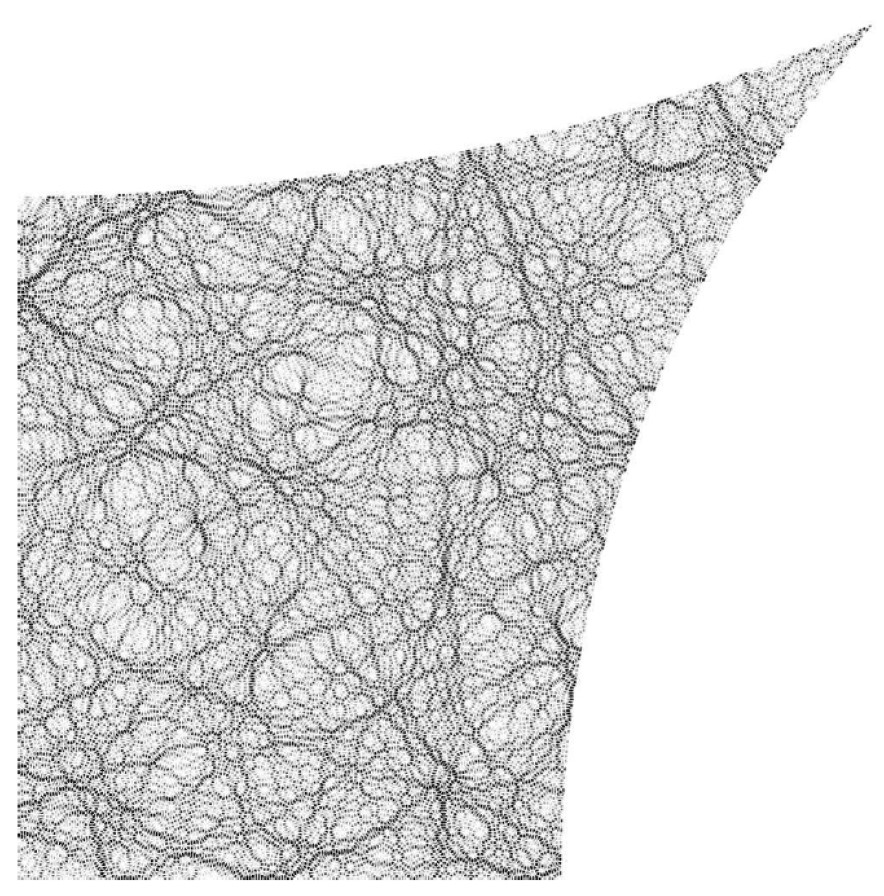
\includegraphics[scale=0.3,angle=0]{Barnett_eig_sim.jpg}
    %\caption{Variabili $X_{n}$}
  %
  \noindent\\
  \decoRule
  \caption{The density eigenfunction $\abs{\vphi_{n}}^{2}$ for $n\simeq5\times10^{4}$ and the corrispondent $\lambda_{n}\simeq10^{6}$. Computed by Alex Barnett.}
  \label{fig:barnett_eigenfunction}
\end{figure}


Barnett examinated these quantities up to $n,m\simeq 7\times10^{5}$, getting a $10^{2}$ improvement of eigenvalue magnitude over the state of art. Moreover, he developed a free \textsc{MatLab} tool to plot efficently eigenfunctions on complex domains (\textsc{mpspack}, see \url{https://github.com/ahbarnett/mpspack}).\\

Another essential support to this field, mainly about Maass forms and quantum chaos problems relative to the modular group and its subgroups arrived, starting from the work of \cite{Hejhal:triang}, recently from Friderik Stromberg (\cite{Stromb:article}), who succeded in calculating the first $10.000$ eigenvalues for $X(1)$. Moreover, Holger Then, with the joint work of already mentioned Barnett, managed to compute and plot eigenfunctions with an high accurancy (\cite{Barnett:asym_rate},\cite{Then:article}).



\begin{figure}[H]
\centering

    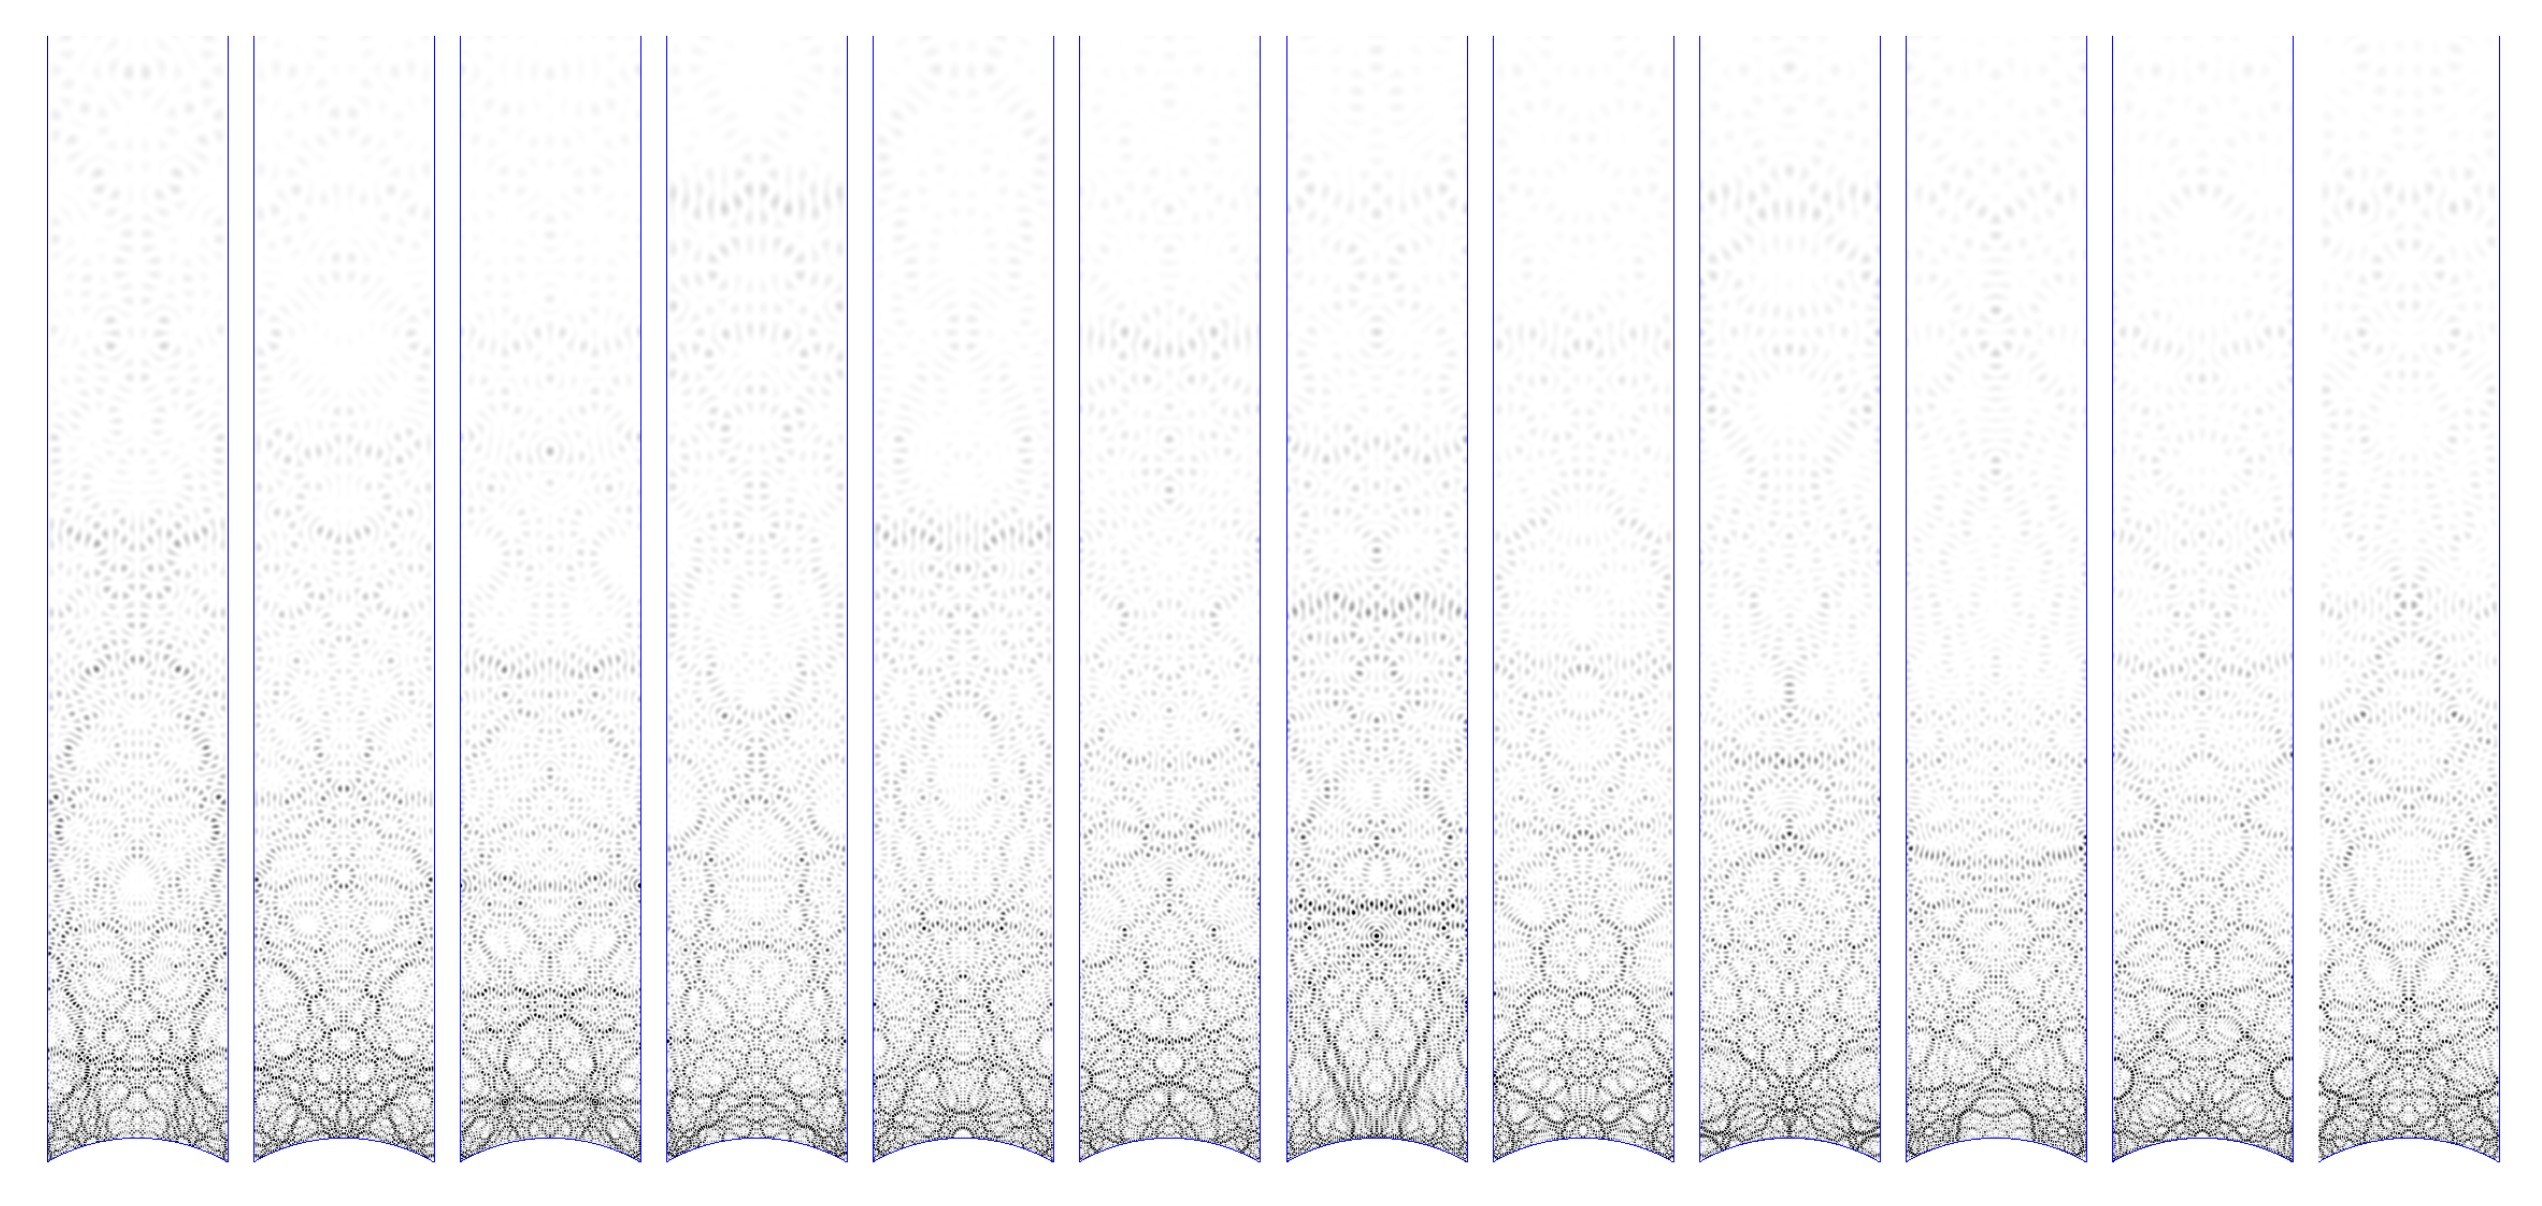
\includegraphics[scale=0.3,angle=0]{mod_surface_then.jpg}
    %\caption{Variabili $X_{n}$}

  %
  \noindent\\

  \decoRule
  \caption{12 consecutive Maass forms (5600th eigenvalue and so on), i.e. laplacian eigenfunctions on the modular surface, computed by Holger Then and Alex Barnett}
  \label{fig:holg_then_eig_modul}
\end{figure}







Not to forget is the breakthroughing contributions due to Strohmaier and Uski, who computed with very high accurancy, the first $1000$ eigenvalues of Laplacian on Bolza surface, using a different algorithm described in \cite{Stroh:comput} best suited for compact surfaces of genus $2,3,4$ (thus very different cases from the modular surface).


\begin{figure}[H]
\centering
  \begin{subfigure}[b]{0.2\textwidth}
  \centering
    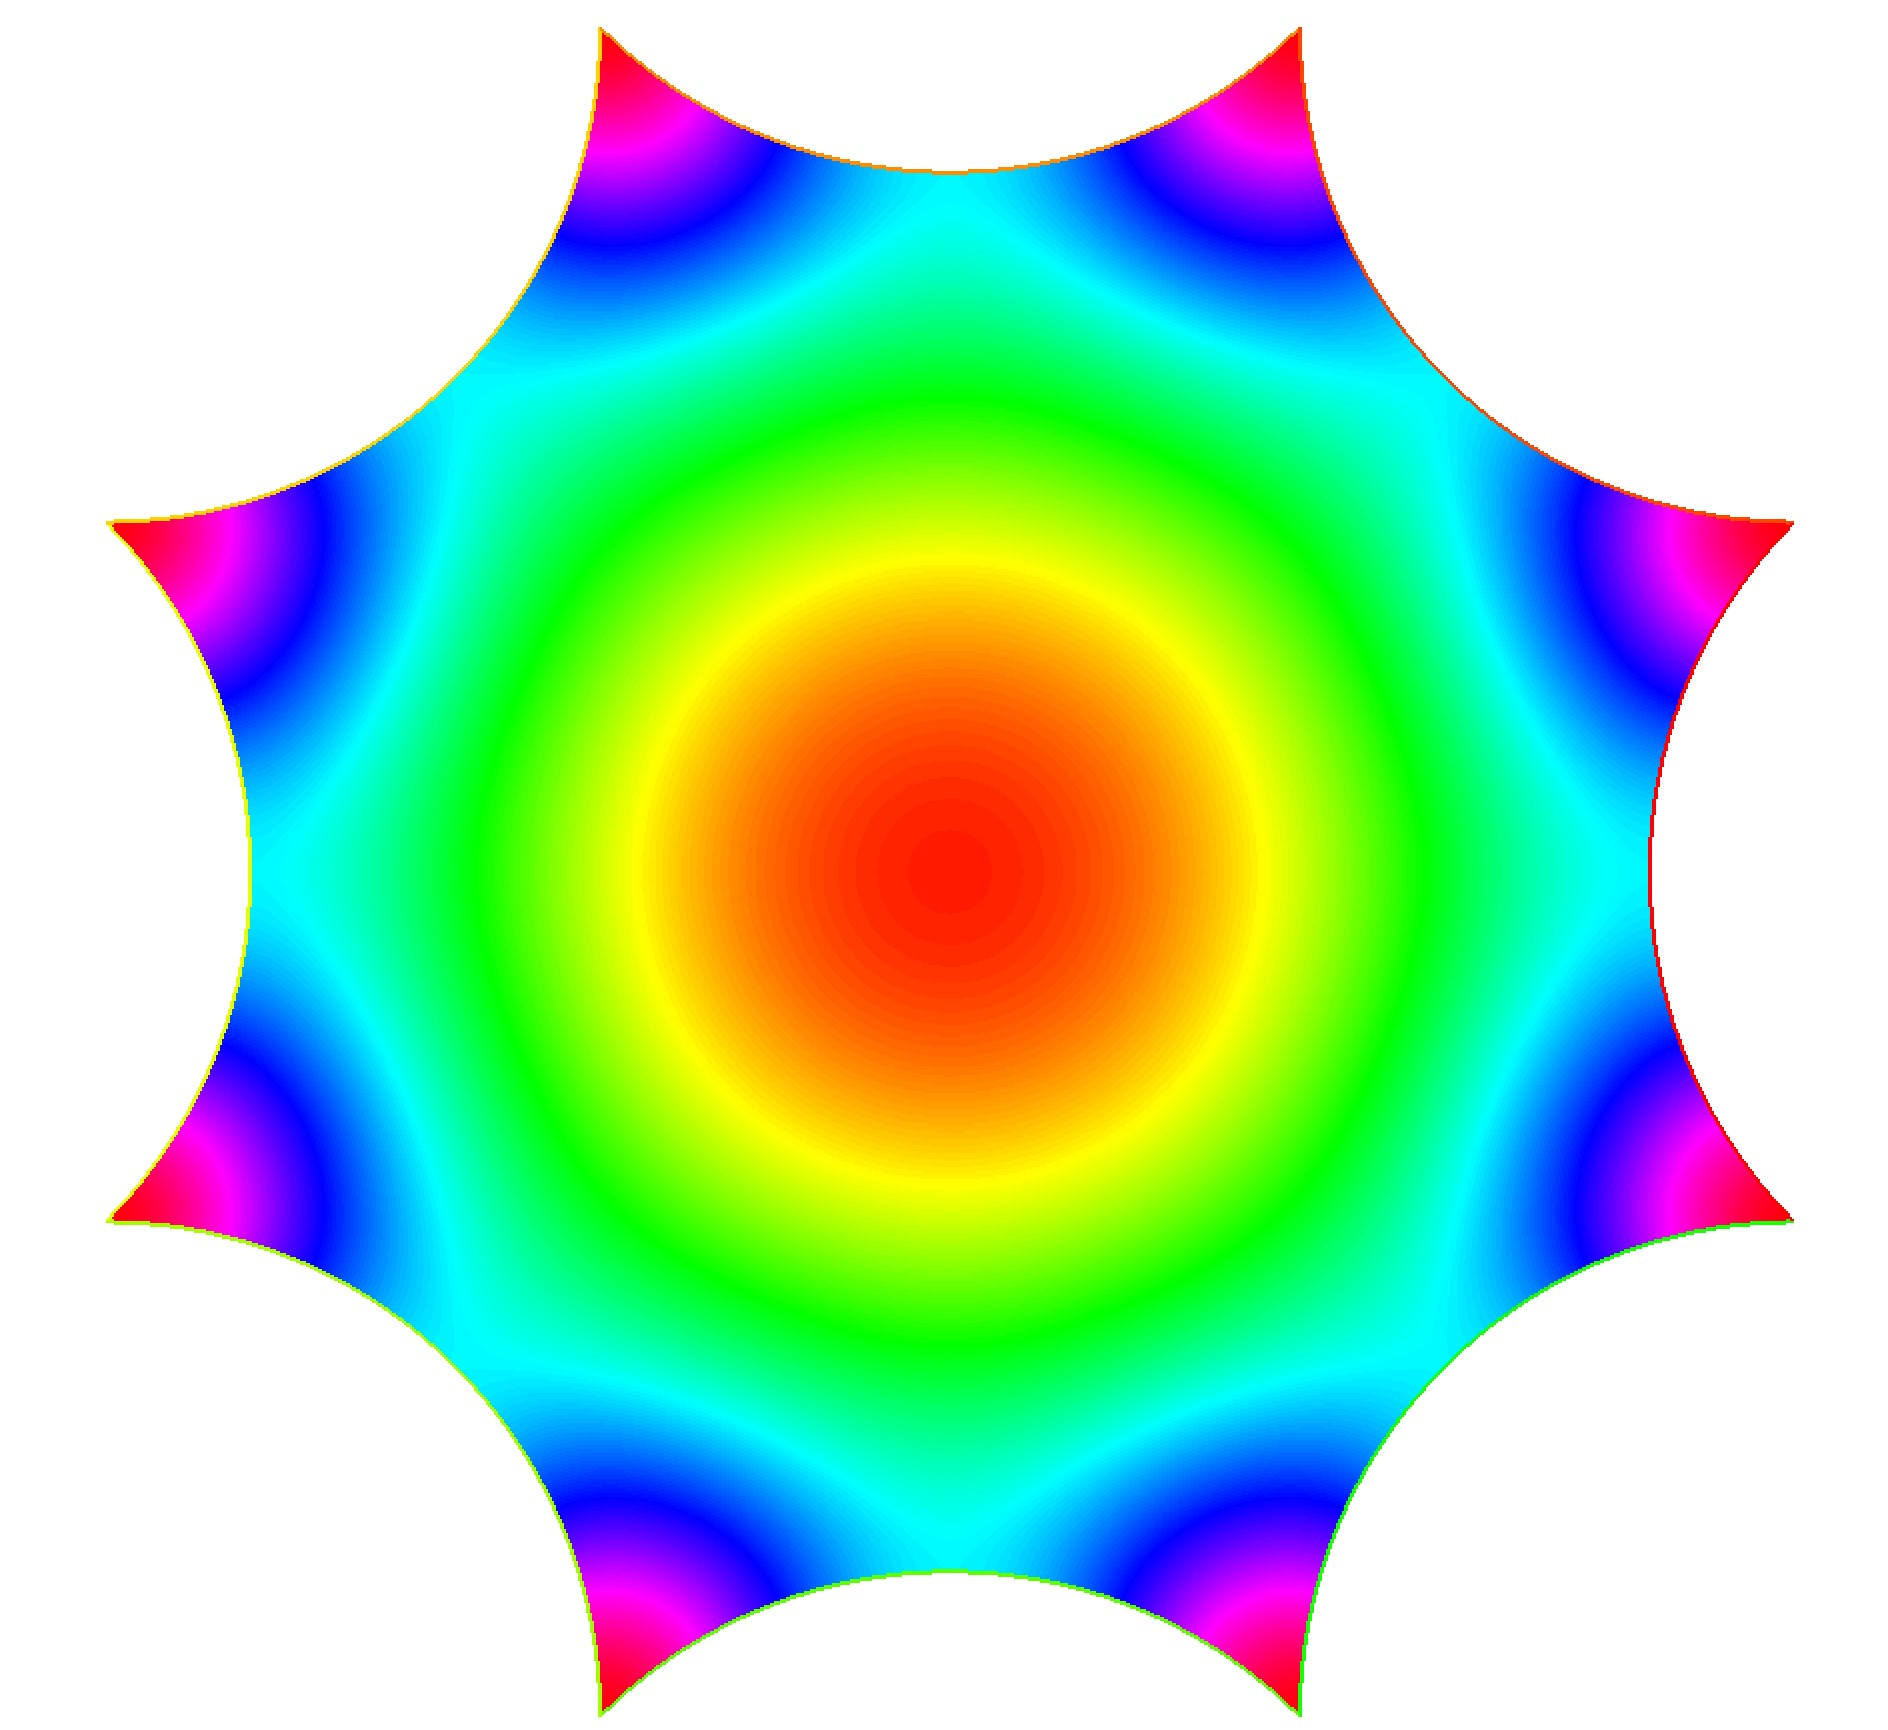
\includegraphics[scale=0.1,angle=0]{bolza1.jpg}
    %\caption{Variabili $X_{n}$}
    \label{fig:eig_bolza1}
  \end{subfigure}
  %
  \noindent\\
  \begin{subfigure}[b]{0.2\textwidth}
  \centering
    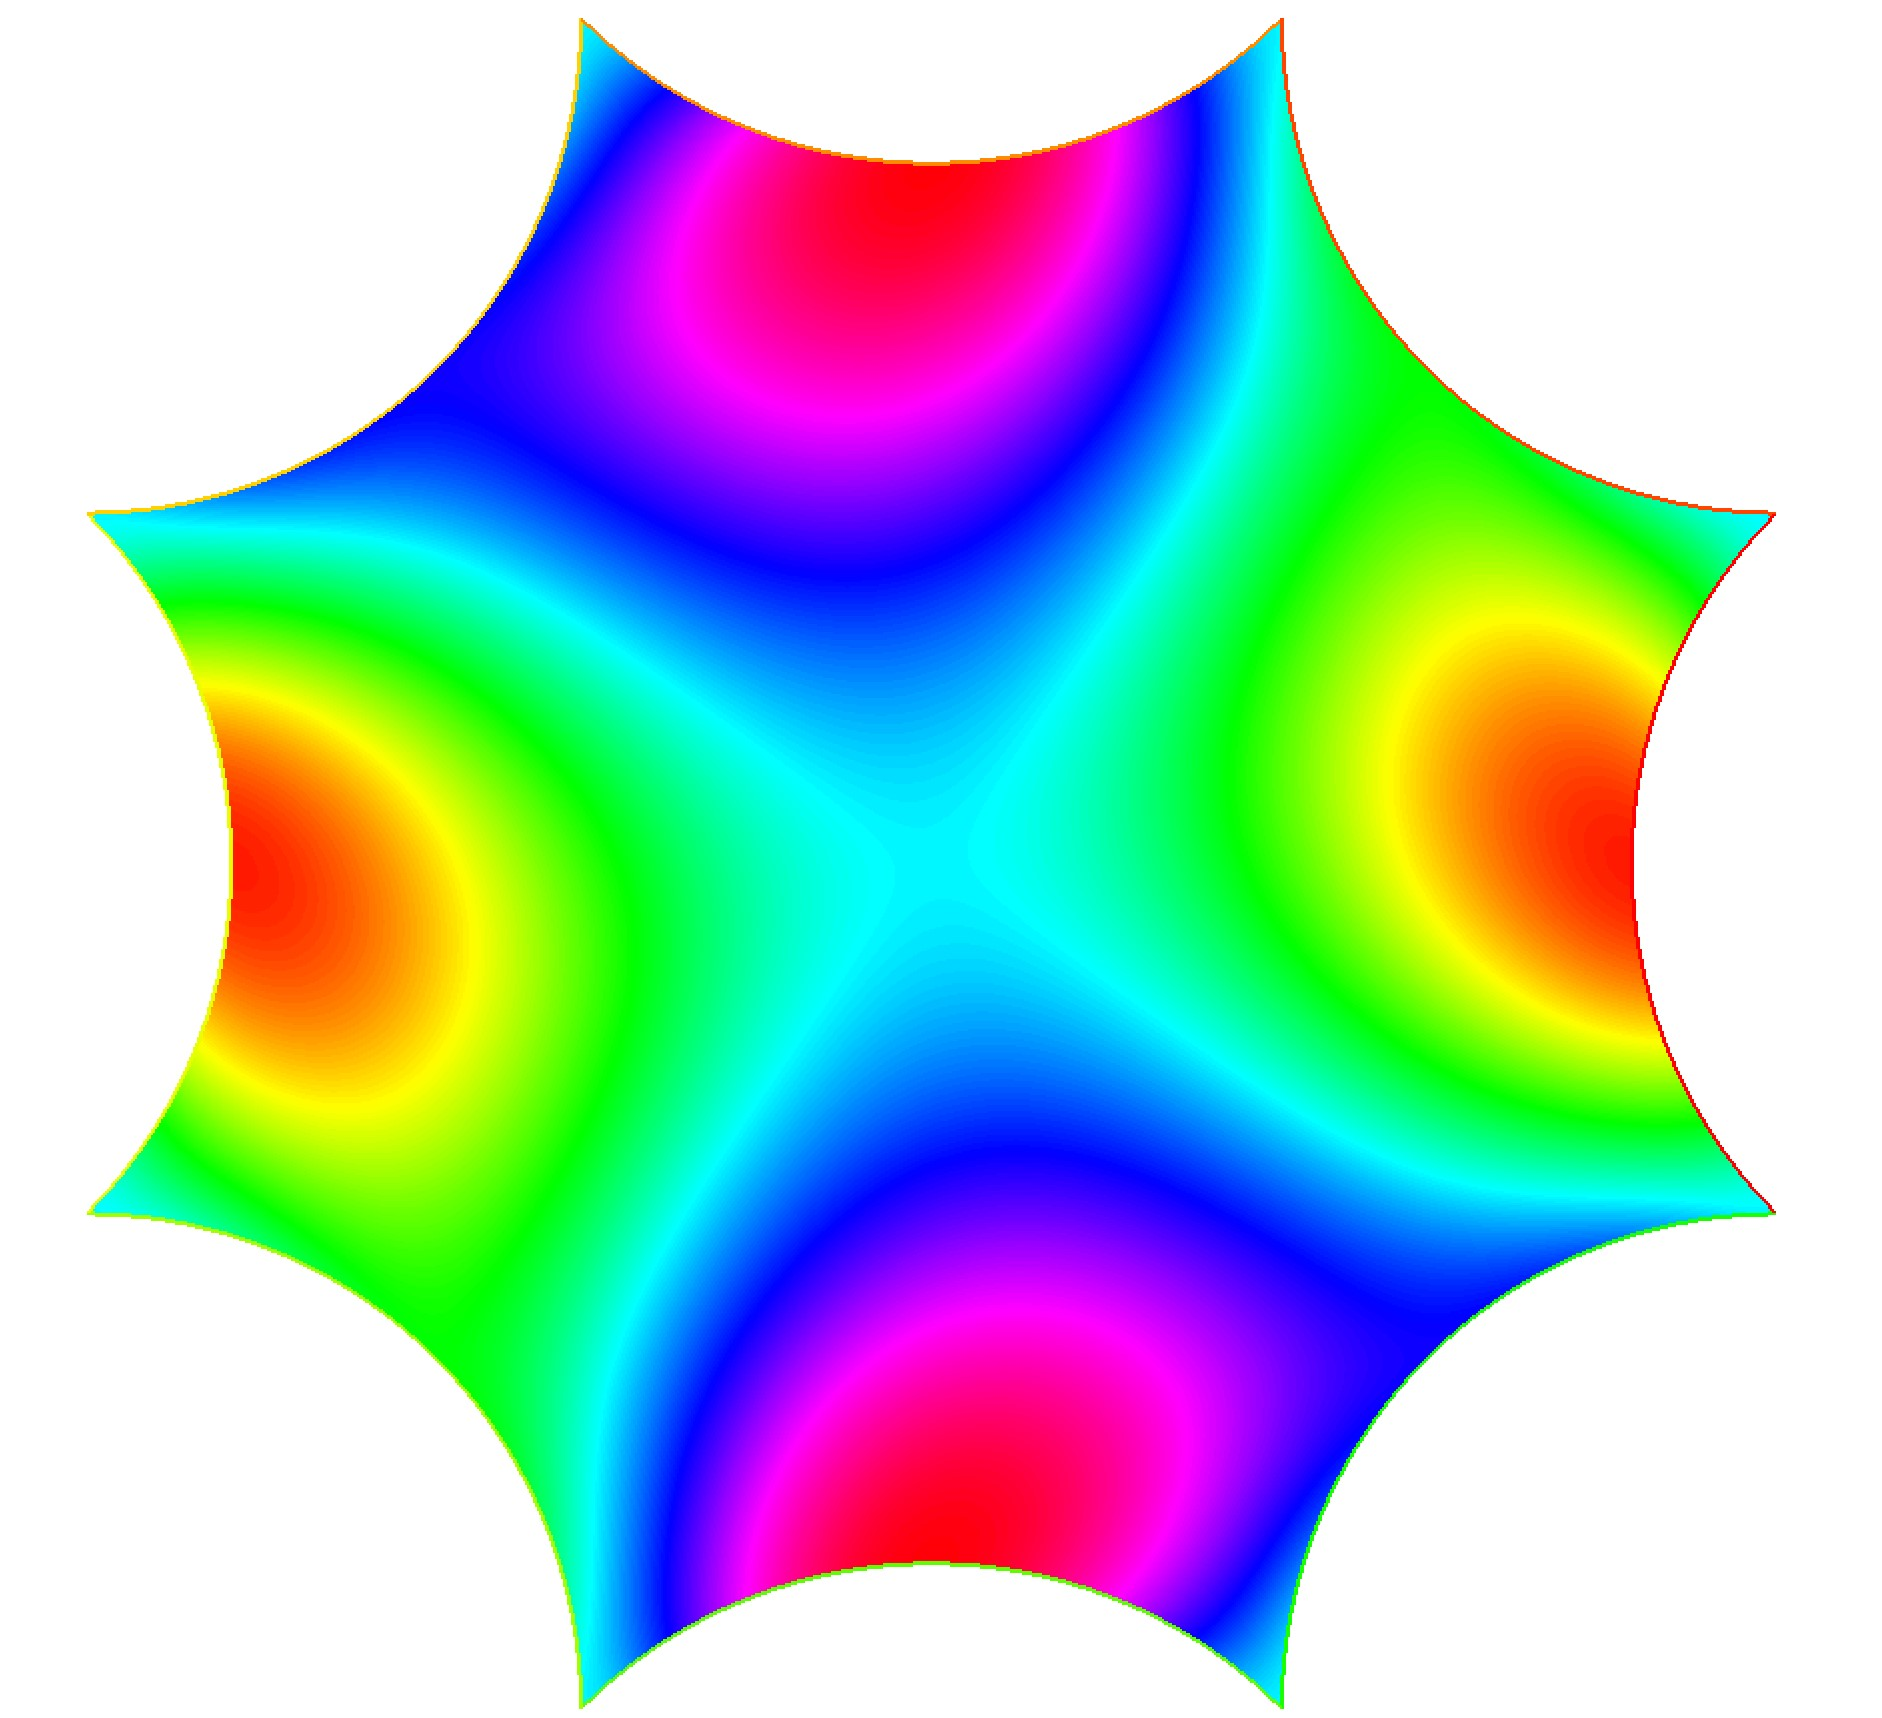
\includegraphics[scale=0.1,angle=0]{bolza2.jpg}
    %\caption{Variabili $X_{n}$}
    \label{fig:eig_bolza2}
  \end{subfigure}
  \begin{subfigure}[b]{0.2\textwidth}
  \centering
    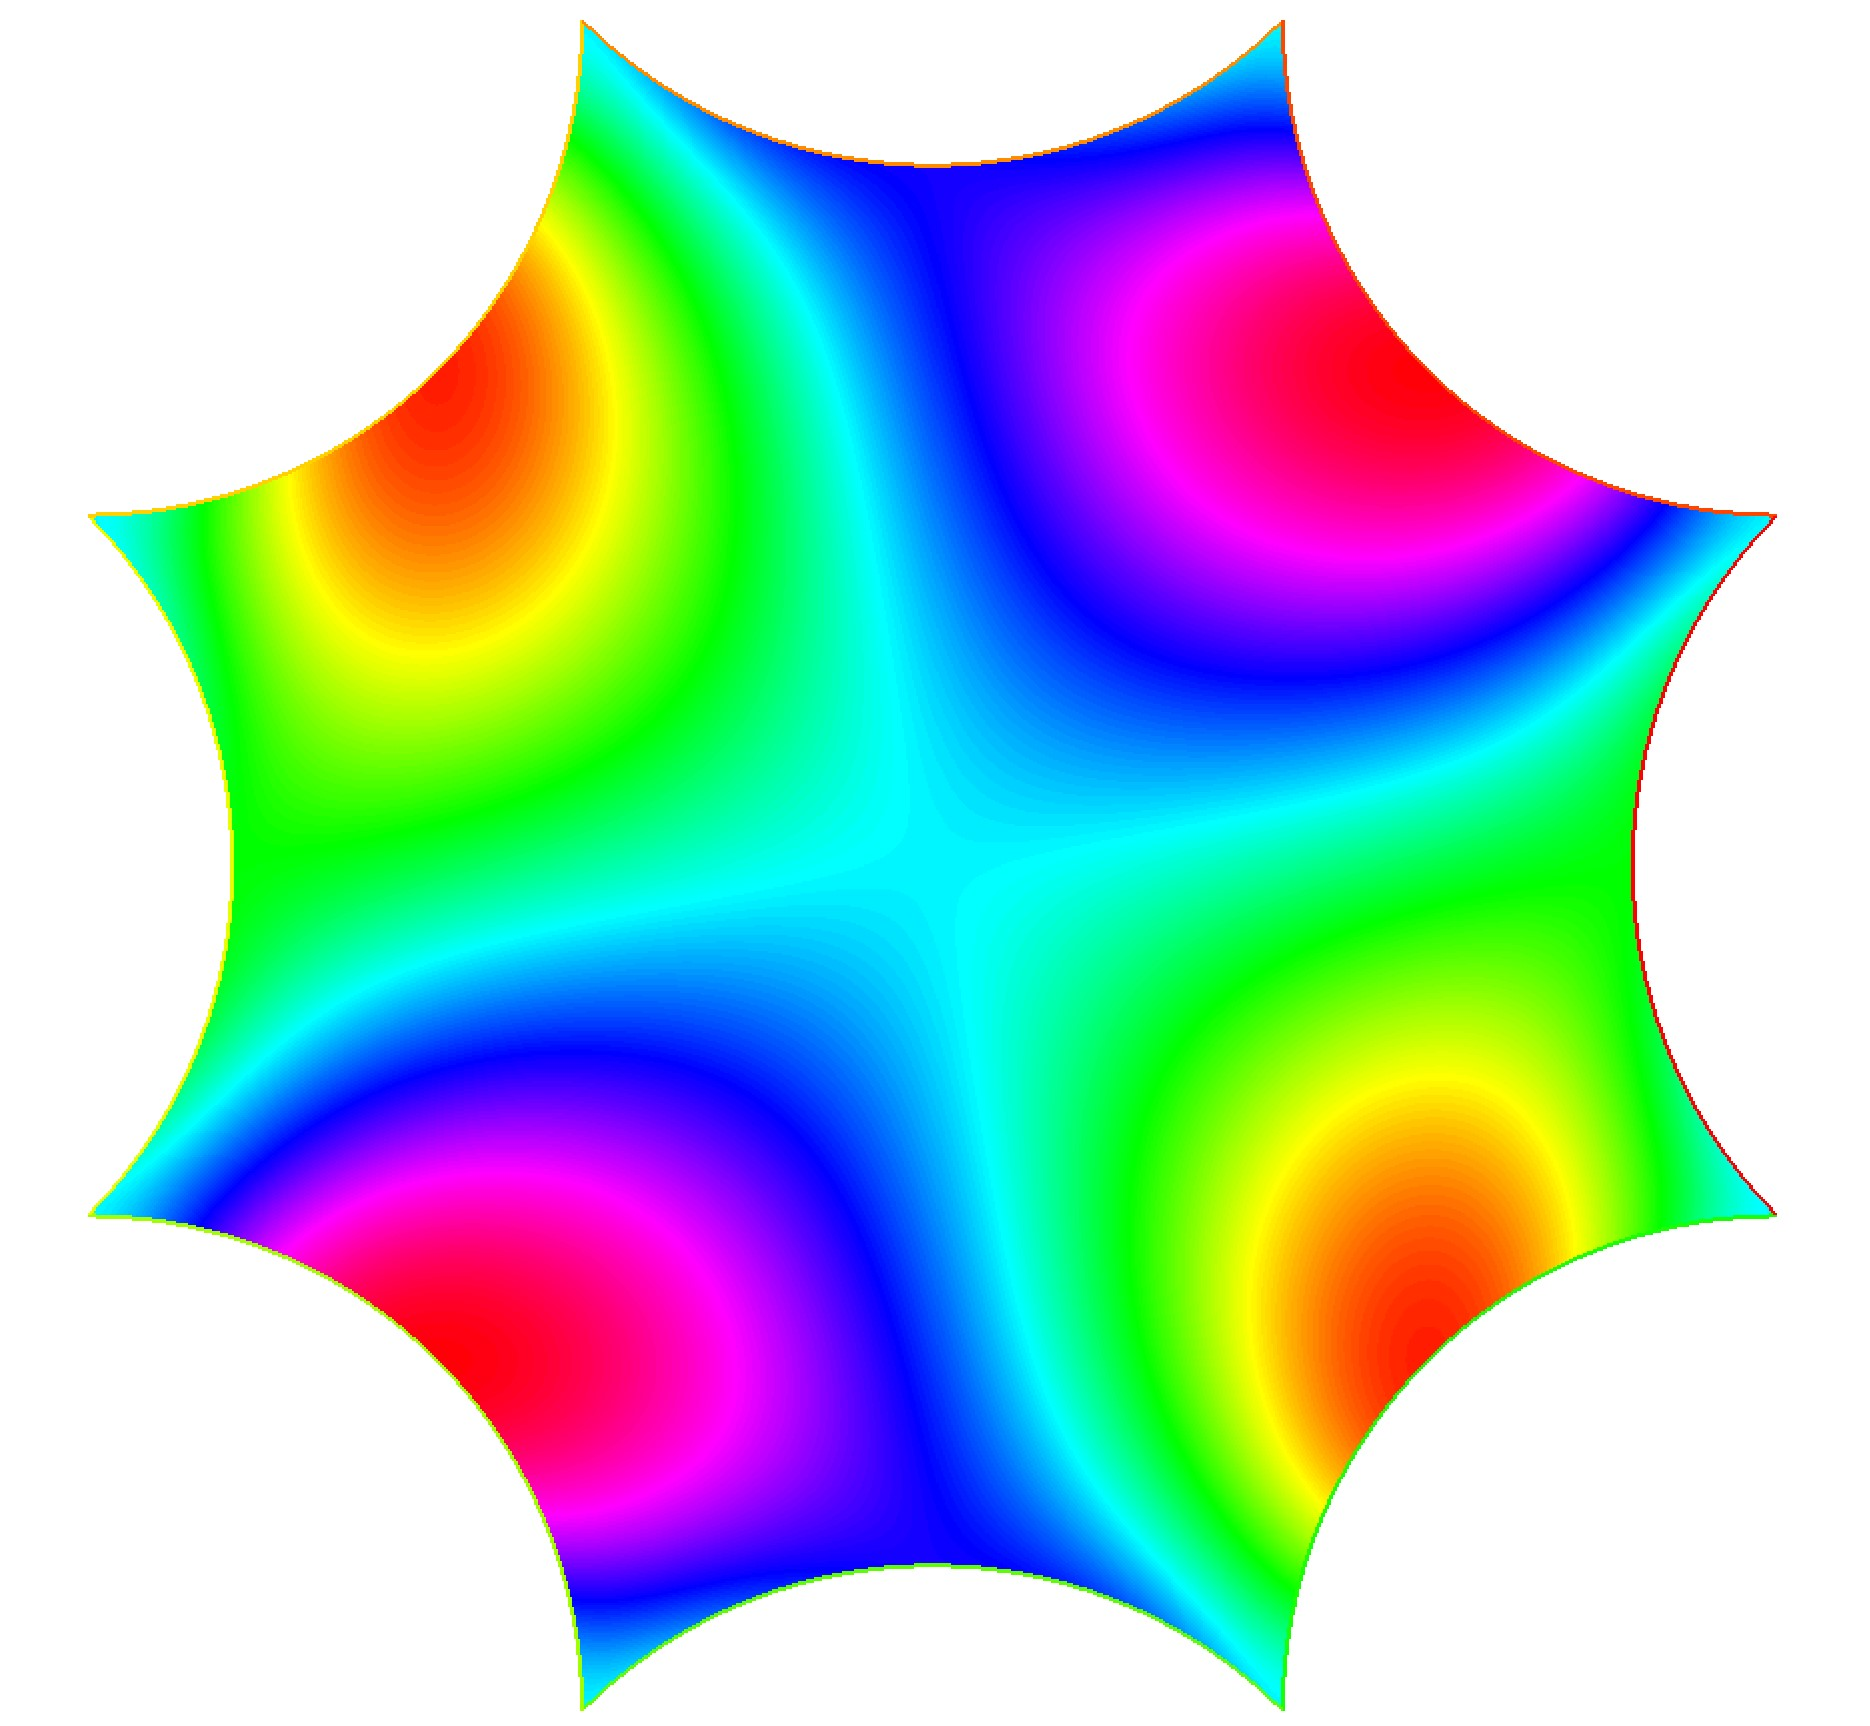
\includegraphics[scale=0.1,angle=0]{bolza3.jpg}
    %\caption{Variabili $X_{n}$}
    \label{fig:eig_bolza3}
  \end{subfigure}
  \noindent\\
  \decoRule
  \caption{The three eigenfunctions on Bolza surface, corrisponding to the first eigenvalue $\lambda=3.8388872\ldots$. See \cite{Stroh:comput}}
  \label{fig:first_3_bolza_eig}
\end{figure}



\begin{figure}[H]
\centering
  \begin{subfigure}[b]{0.2\textwidth}
  \centering
    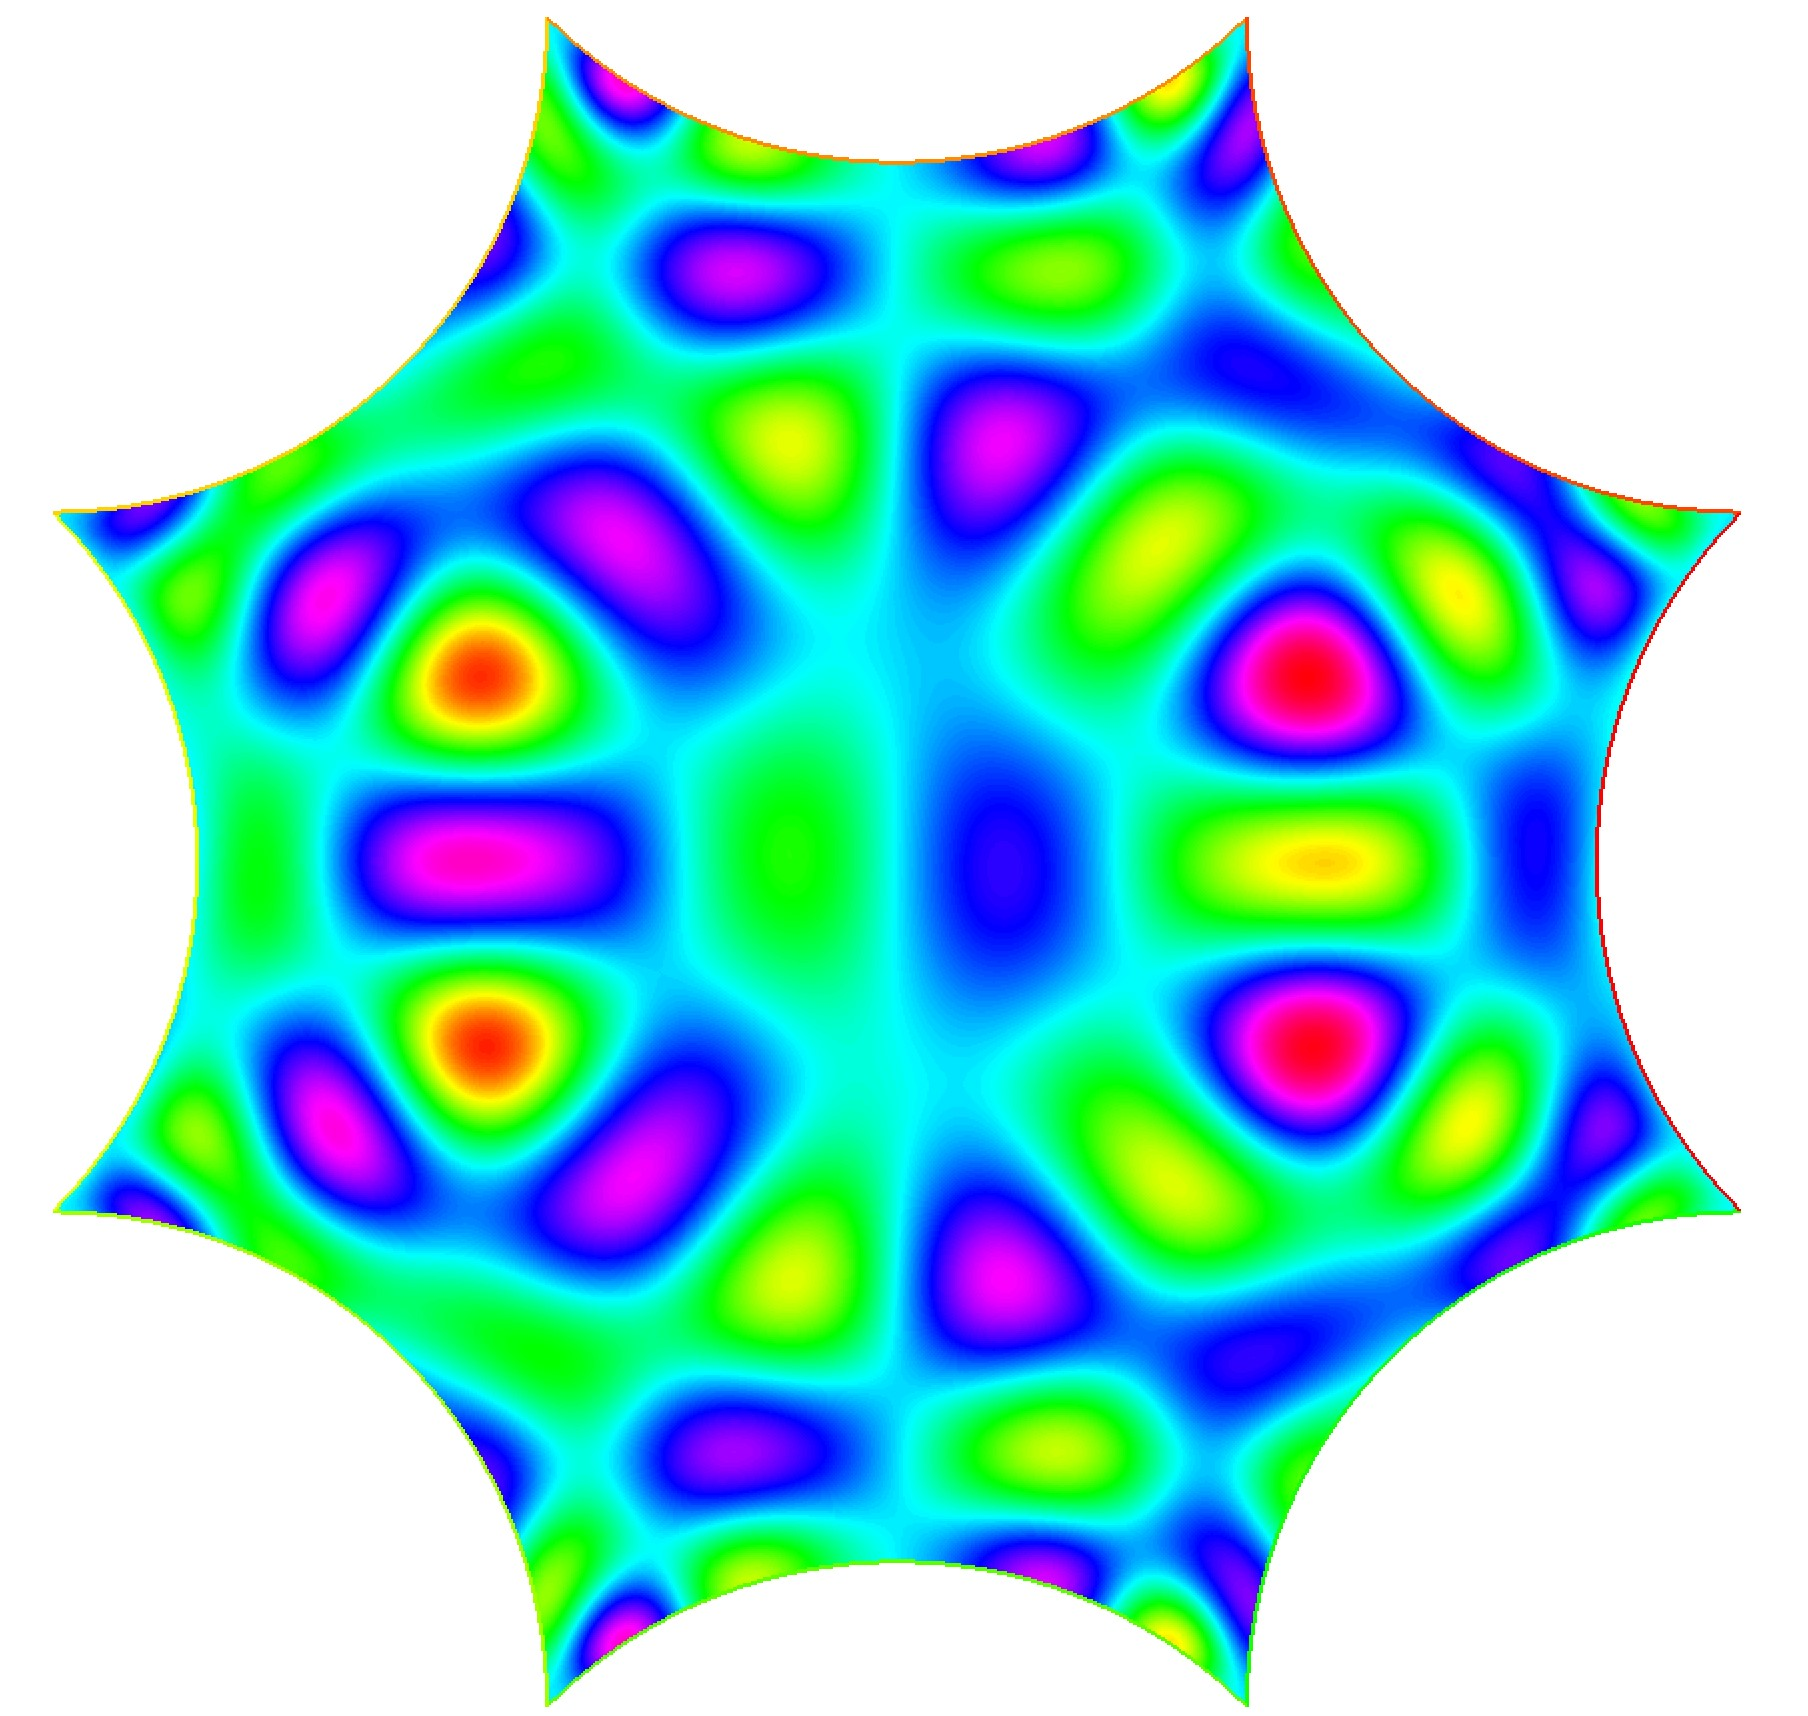
\includegraphics[scale=0.08,angle=0]{bolza5.jpg}
    %\caption{Variabili $X_{n}$}
    \label{fig:eig_bolza4}
  \end{subfigure}
  %
  \begin{subfigure}[b]{0.2\textwidth}
  \centering
    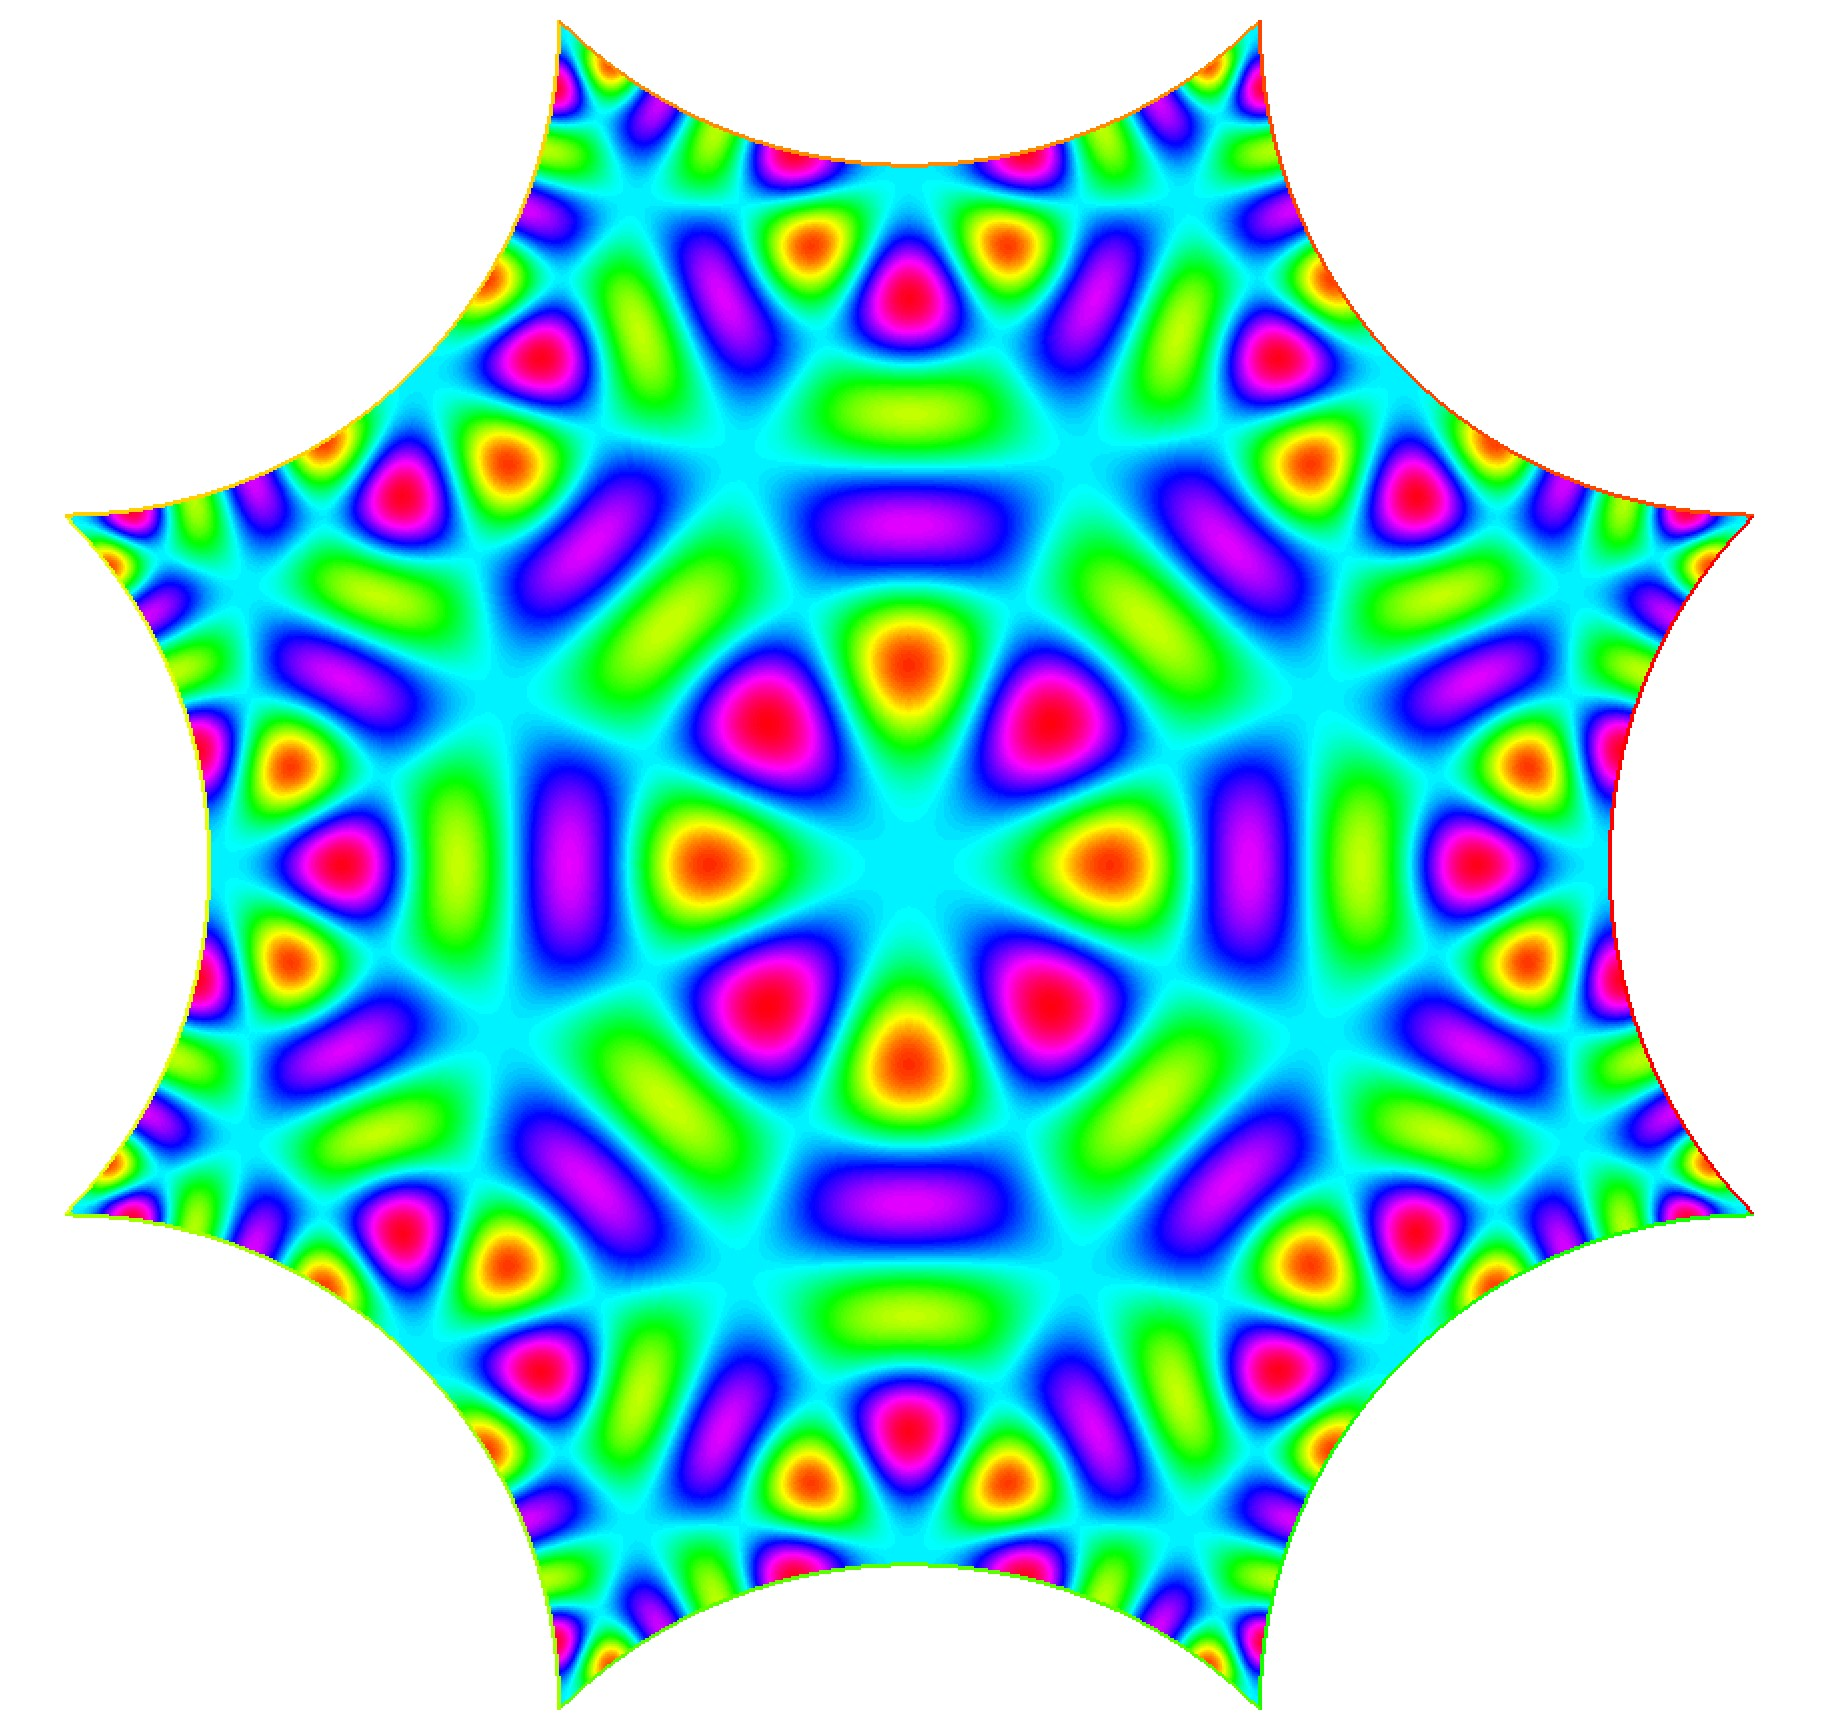
\includegraphics[scale=0.08,angle=0]{bolza6.jpg}
    %\caption{Variabili $X_{n}$}
    \label{fig:eig_bolza5}
  \end{subfigure}
  \begin{subfigure}[b]{0.2\textwidth}
  \centering
    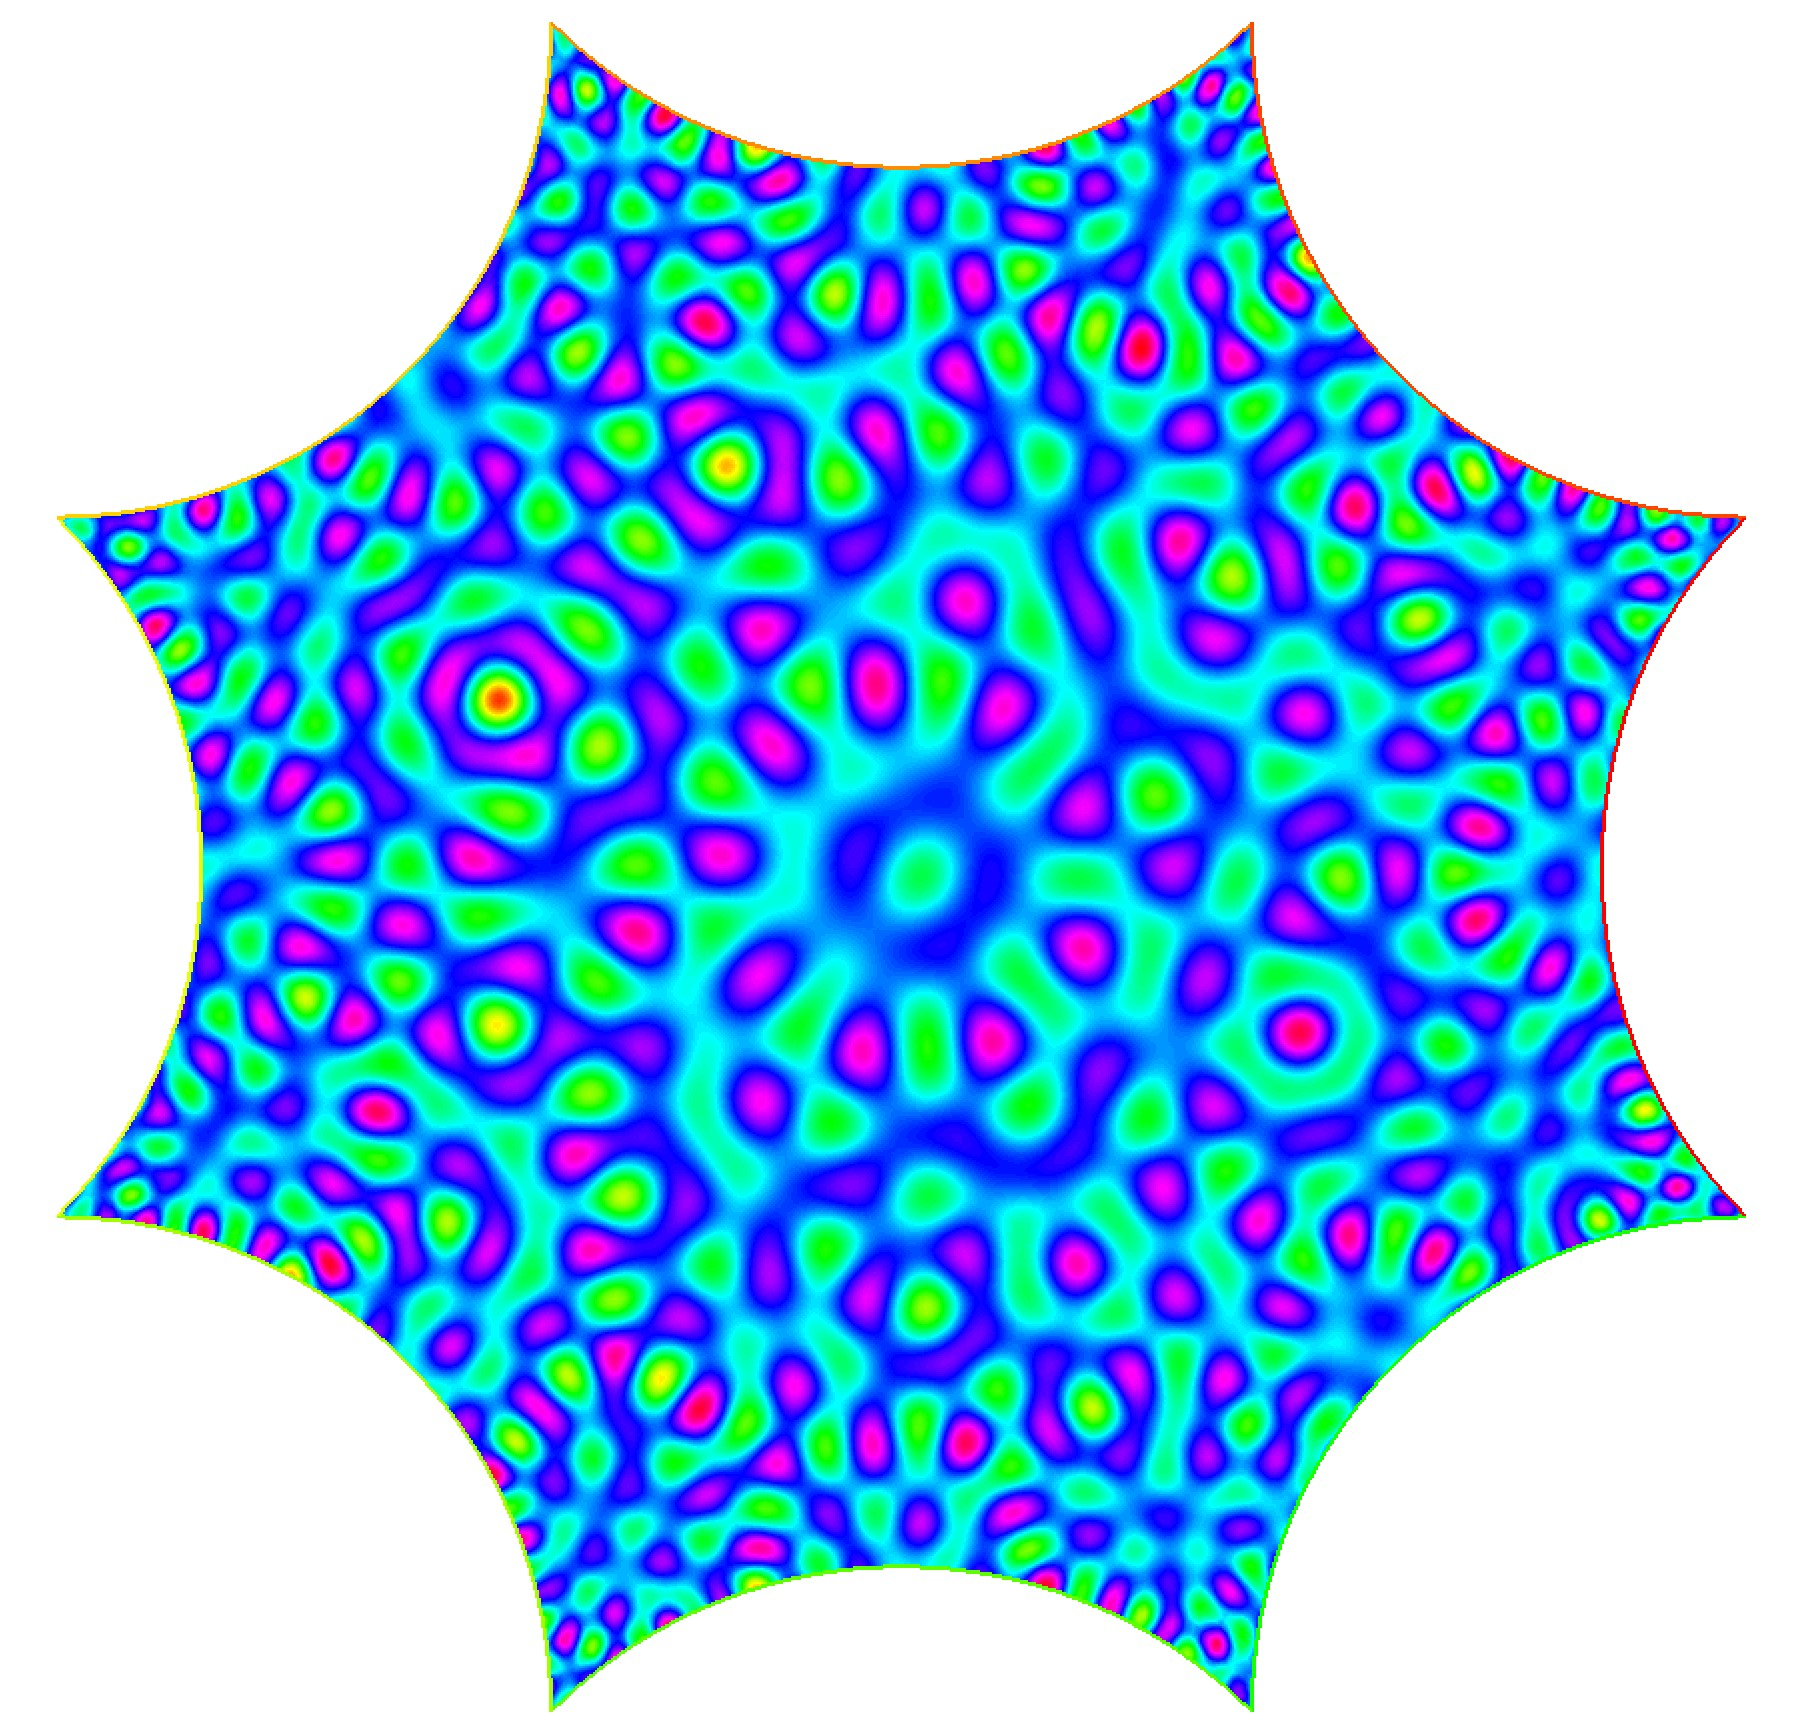
\includegraphics[scale=0.08,angle=0]{bolza7.jpg}
    %\caption{Variabili $X_{n}$}
    \label{fig:eig_bolza6}
  \end{subfigure}
    \begin{subfigure}[b]{0.2\textwidth}
  \centering
    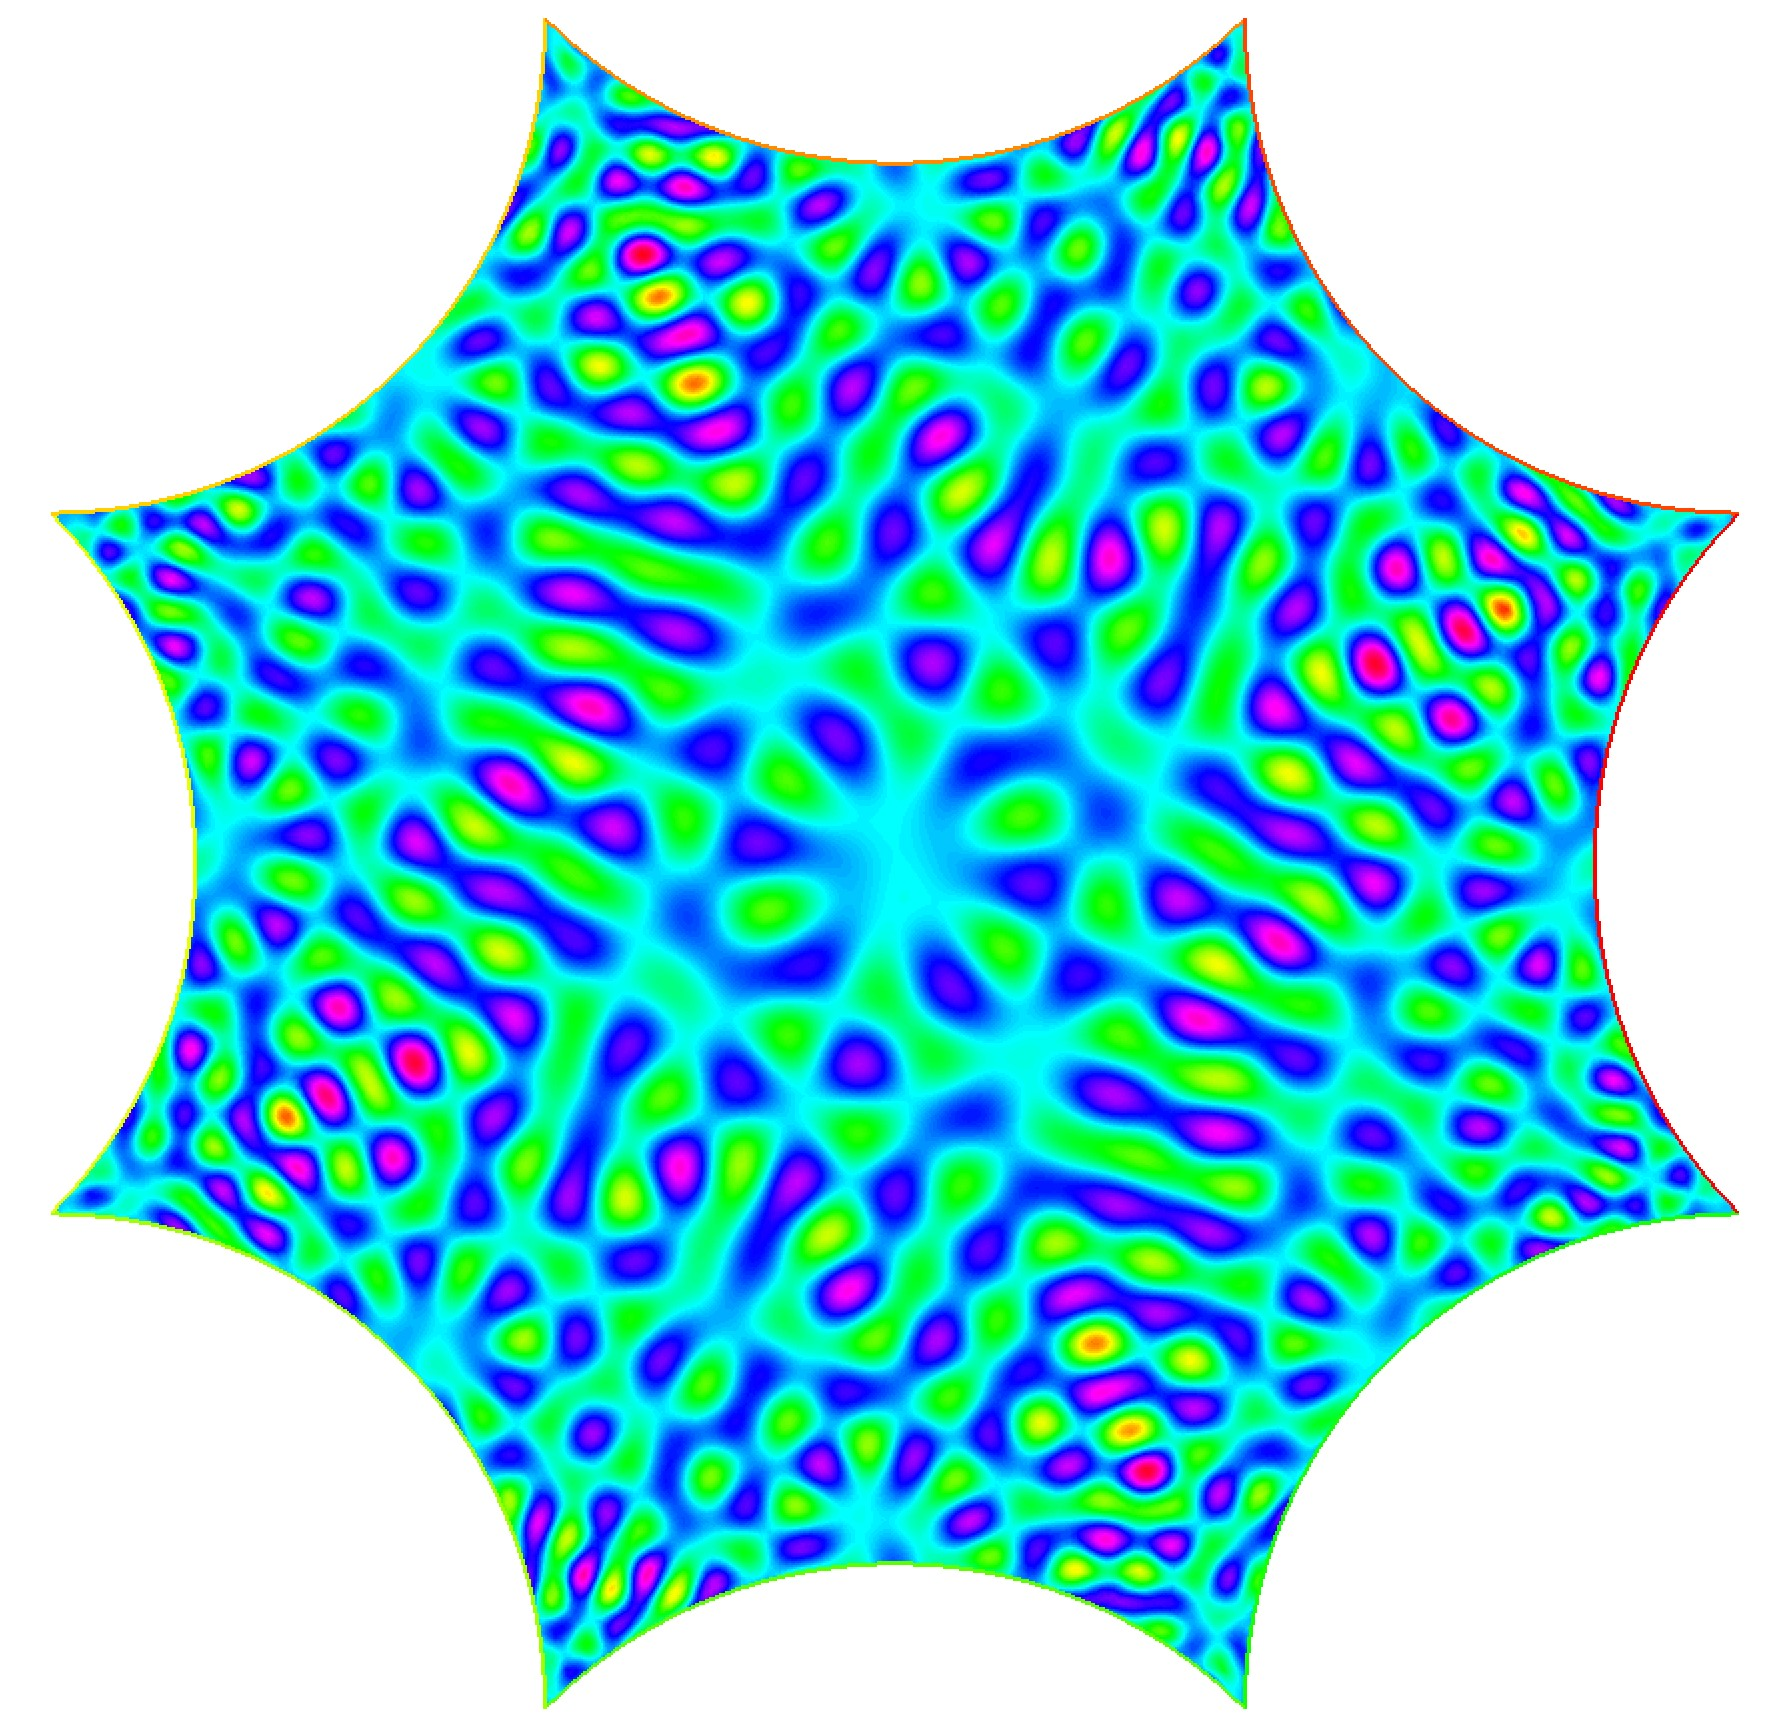
\includegraphics[scale=0.08,angle=0]{bolza8.jpg}
    %\caption{Variabili $X_{n}$}
    \label{fig:eig_bolza7}
  \end{subfigure}
  \noindent\\
  \decoRule
  \caption{Bolza surface is an arithmetic hyperbolic surface, thus eigenfunctions equidistributes on the surface.}
  \label{fig:bolza_eig_equidistr}
\end{figure}



\begin{figure}[H]
\centering
  \begin{subfigure}[b]{0.4\textwidth}
  \centering
    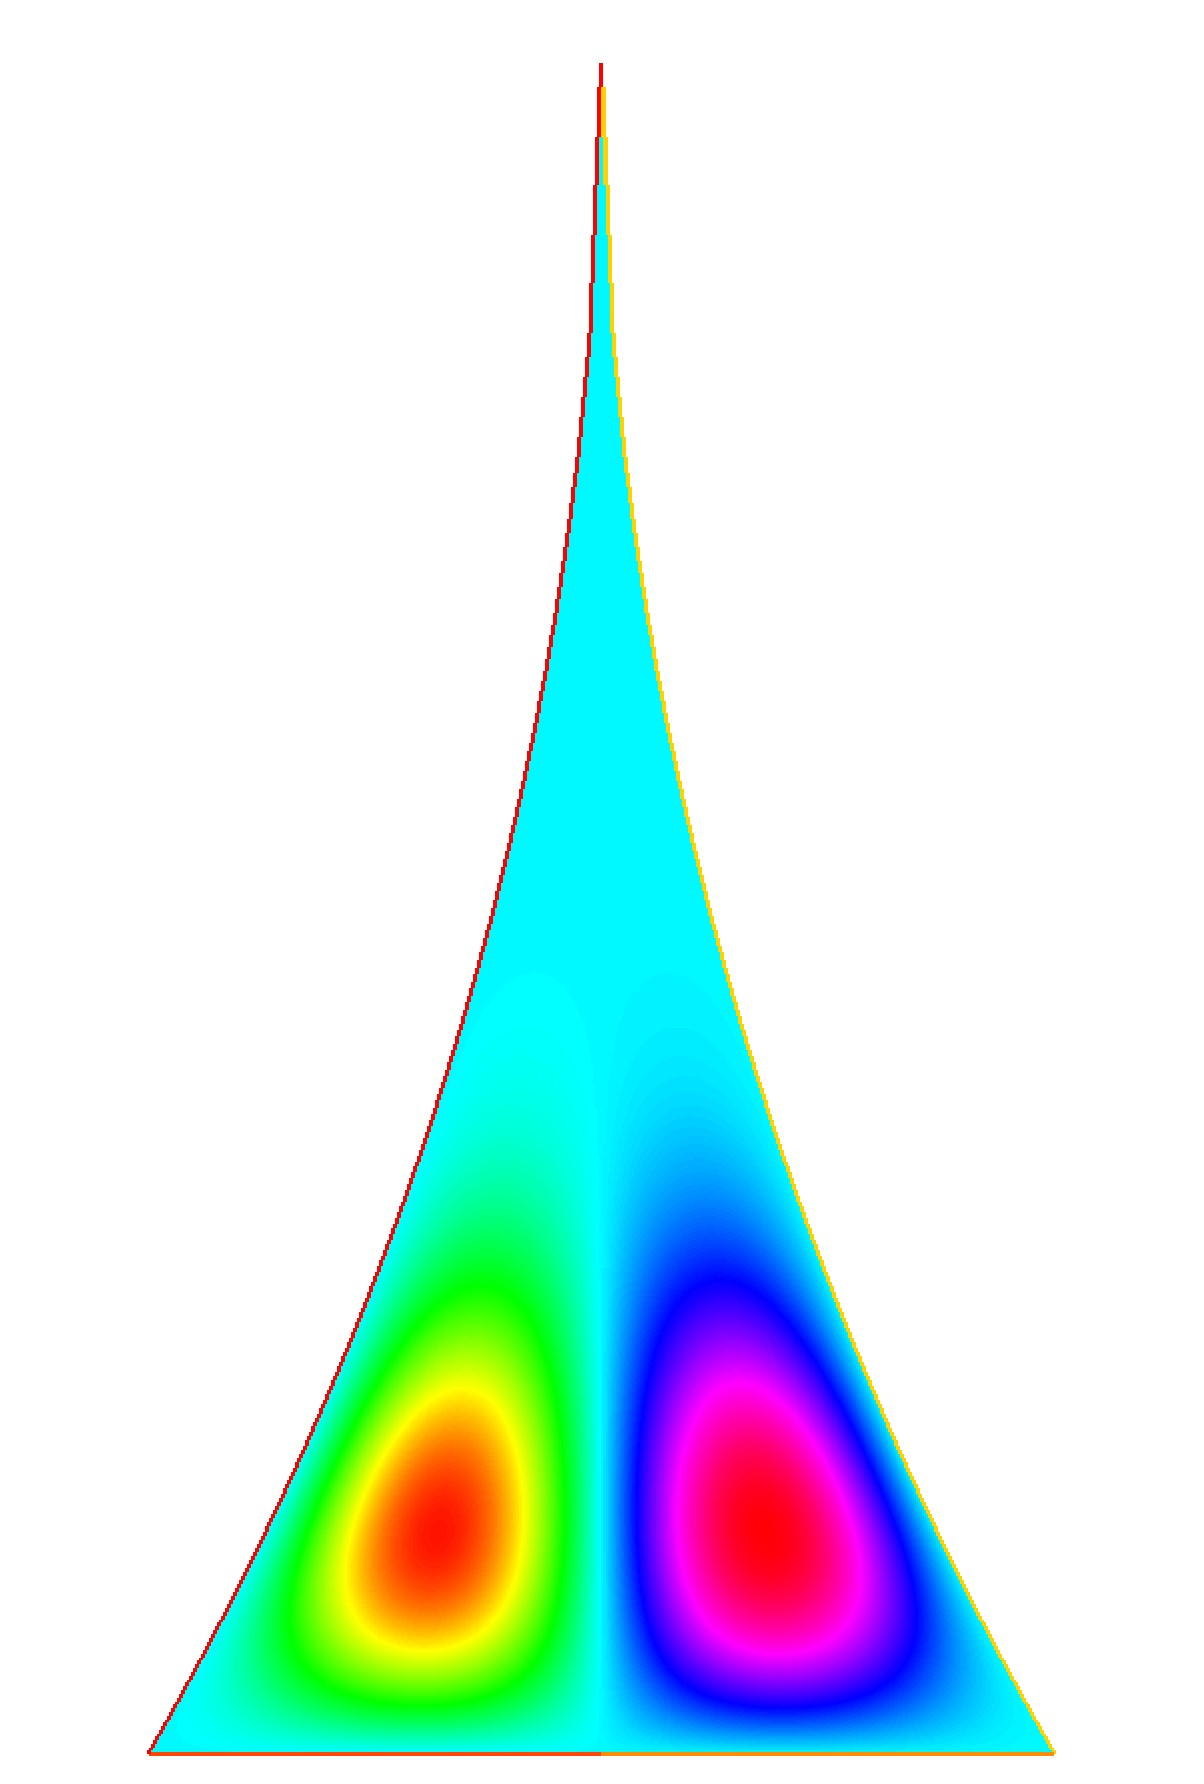
\includegraphics[scale=0.15,angle=0]{modular1.jpg}
    %\caption{Variabili $X_{n}$}
    \label{fig:modular_eig1}
  \end{subfigure}
  %
  \begin{subfigure}[b]{0.4\textwidth}
  \centering
    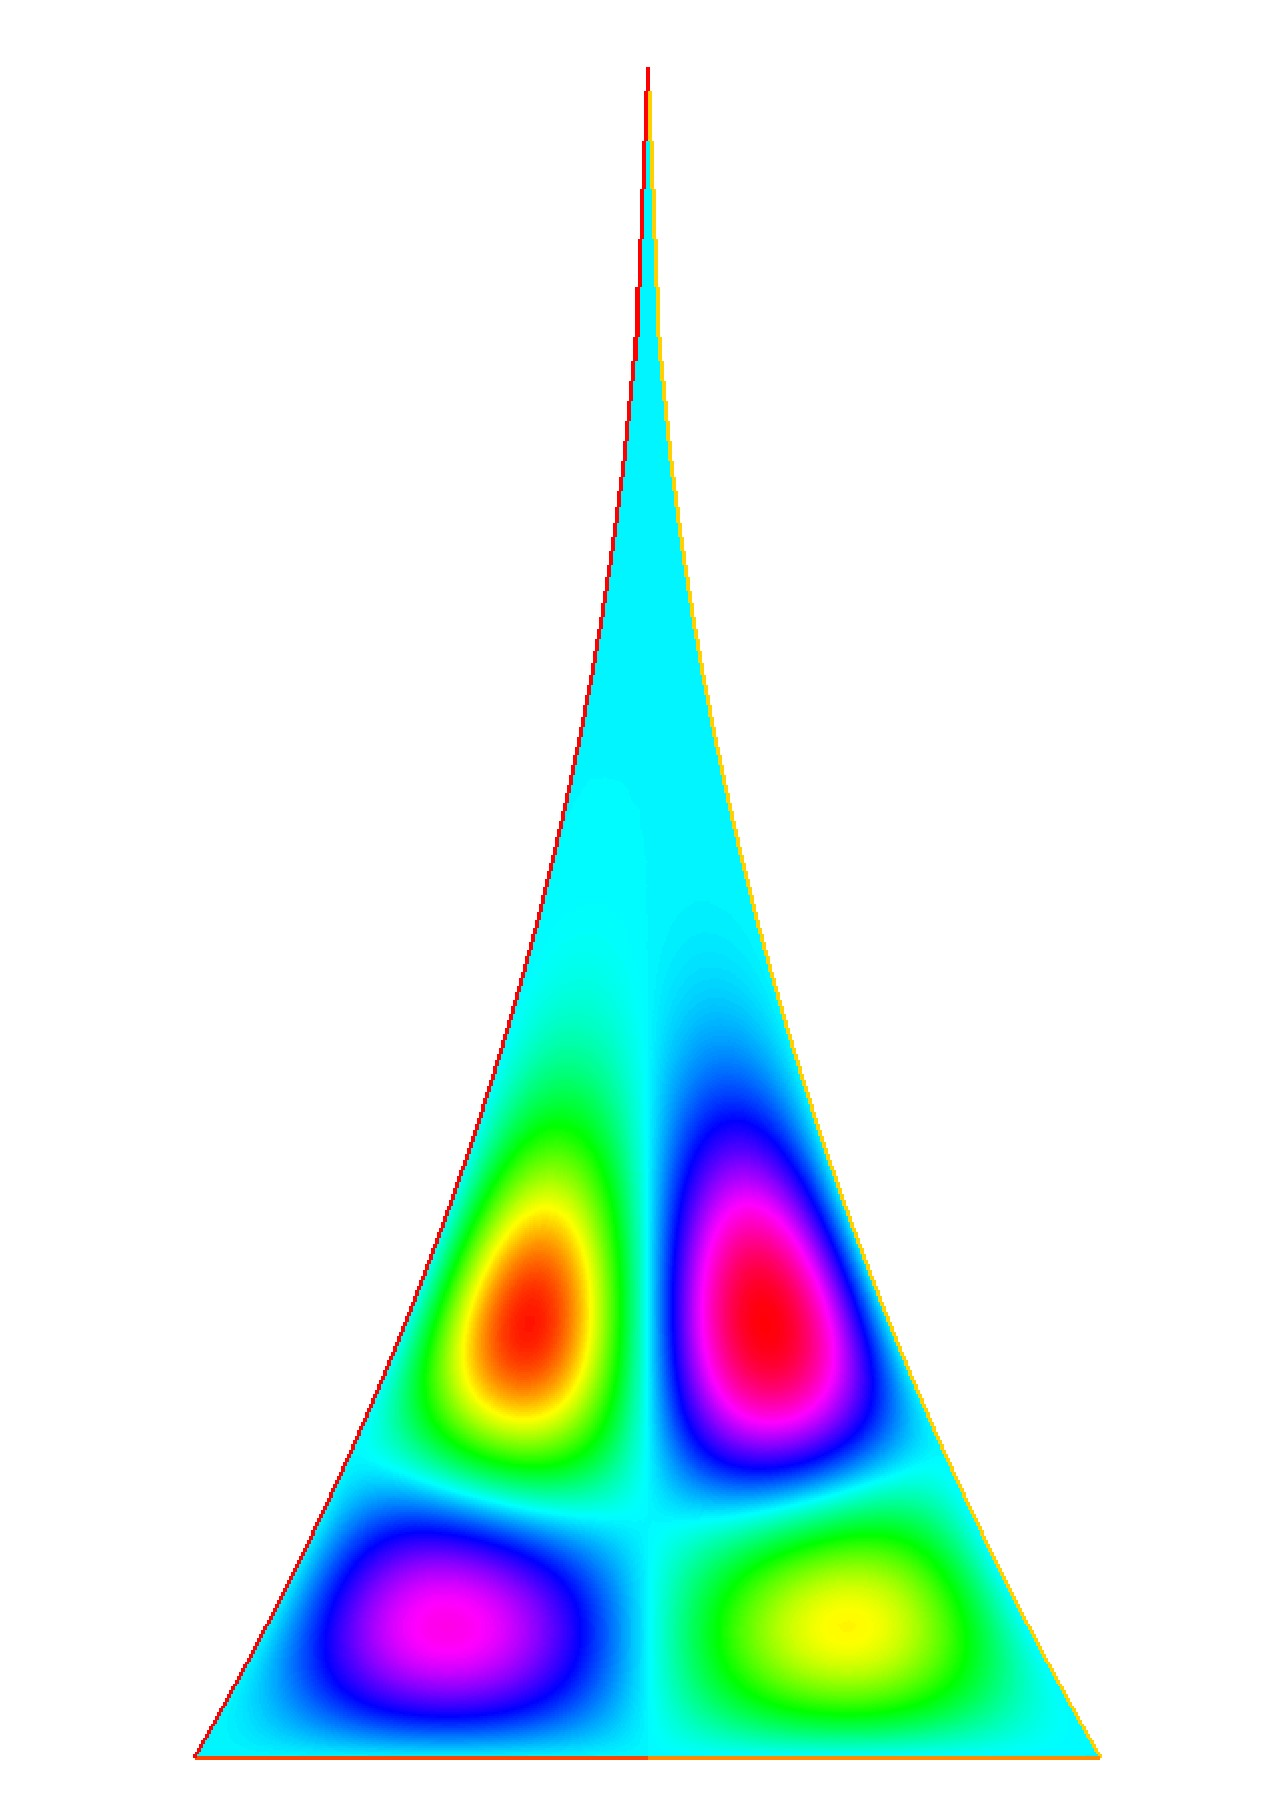
\includegraphics[scale=0.15,angle=0]{modular3.jpg}
    %\caption{Variabili $X_{n}$}
    \label{fig:modular_eig2}
  \end{subfigure}
  \noindent\\
  \decoRule
  \caption{The first two eigenfunctions of the modular surface, see on the Poincaré disk model $\Disk$. The corrisponding eigenvalues are $\lambda_{1}=91.12\ldots$ and $\lambda_{2}=148.43\ldots$, see \cite{Sarnak:review}.}
  \label{fig:first_two_eig_modular}
\end{figure}



METTI  ALTRE FIGURE EIGENFUNCTIONS FATTE DA TE 


\subsection{Numerical methods}

The first attempts to investigate the spectrum of the modular surface $X(1)$ were carried out in \cite{Cart:comput}. After those not-so-successfully attemps, other simulations were made and, among the eigenvalues $1/4+t^{2}=\lambda$, some Riemann zeros $1/2+\imi t$ suddenly appeared. The reason was later discovered by Hejhal \cite{Hejhal:triang}, who also developed a useful (heuristic) method to compute spectra of modular surfaces, and later improved by the already mentioned Friderik Stromberg, in his PhD thesis.\\

The reason behind the presence of Riemann zeta's zeros was the following: the numerical methods used until then were faulty in allowing the eigenfunctions to have logarithmic singularities. Obviously, these were not real eigenfunctions. The method developed by Heijal is now known as \virg{collocation}. The eigenfunctions, i.e. cusp forms, considered have a Fourier expansion in $z=x+\imi y$ given by 
\[
\vphi^{+}(z)=\sum_{n=1}^{\infty}\rho_{\vphi}(n)y^{1/2} K_{\imi t_{\vphi}}(2\pi ny)\cos(2\pi nx)
\]
and
\[
\vphi^{-}(z)=\sum_{n=1}^{\infty}\rho_{\vphi}(n)y^{1/2} K_{\imi t_{\vphi}}(2\pi ny)\sin(2\pi nx)
\]
where $\vphi^{\pm}(z)$ are, respectively, even and odd eigenfunctions respect to the vertical axis $\Re(z)=0$ (see \cite{Stark:mod_forms},\cite{Sarnak:review} for details) and the eigenvalue is $\lambda=1/4+t^{2}_{\vphi}$.\\
The unknowns in these expressions are the coefficients $\rho_{\vphi}(n)$ and the eigenvalue parameter $t_{\vphi}$. We will roughly described a main method un this subject, due to Heijal, which is suited for \virg{not-so-big} eigenvalue parameters $t_{\vphi}$, but there are other modern methods, due to Stark, Barnett, Stromberg and Strohmaier among the others, which cover different cases.\\

The Bessel function $K_{\imi t_{\vphi}}(y)$ is exponentially decreasing for $y\gg\abs{t_{\vphi}}$, so that the series expressing $\vphi^{\pm}$ is approximated with an accurancy of $O(\e^{-2\pi M})$ for $y\geq\frac{\sqrt{3}}{2}$, when both series are truncated at $n=M$. The functions $\vphi(z)$ are already $1$-periodic\footnote{The eigenfunctions have to be $\PSL_{2}\Z$-invariant and $\PSL_{2}\Z=\spn{J,S}$, where $Jz=-1/z$ and $Sz=z+1$, see section \ref{subsec:hyp_surfc}.} so what is missing is the $J$-invariance, i.e. the condition $\vphi(-1/z)=\vphi(z)$.\\
This method is \virg{good} to get eigenvalues of $X(1)$ such that $\lambda\lesssim 250000$. At first, truncate the series at $n=M$ and choose evenly distributed points $z_{1},\ldots,z_{M}\in D_{2\imi}$ ($z_{i}=x_{i}+\imi y_{i}$), where $D_{2\imi}$ is the Dirichlet fundamental domain of $X(1)$ with center $2\imi$. The condition $\vphi(-1/z)=\vphi(z)$ for the truncated series $\vphi^{(M)}(z)$ and the chosen sample gives the system of equations
\[
\vphi^{(M)}(z_{j})=\vphi^{(M)}(-1/z_{j}),\forall i=1,\ldots, M
\] 
which is a homogeneous linear system of $M$ equations with $M$ unknowns. Each equation is of the form
\[
\sum_{n=1}^{M}\rho(n)A_{n,j}(t)=0
\]
where\footnote{We consider the even case for $\vphi$.}
\[
A_{n,j}(t)=A_{n}(z_{j},t)\coloneqq\sqrt{Jy_{j}}K_{\imi t}(2\pi n Jy_{j})\cos(2\pi nJx_{j})-\sqrt{y_{j}}K_{\imi t}(2\pi n y_{j})\cos(2\pi nx_{j}).
\]
One way to go on, at this point, is to seek solutions $t\leq T$ of the equation 
\[
\det A(t)=0
\]
where $A$ is the matrix obtained by elements $A_{n,j}(t)$. However, to speed up the process it is more convenient to choose a second set of points $w_{2},\ldots,w_{M}$ and to solve the double system of equation (setting $\rho(1)=1$)
\begin{equation}
\label{eq:system_heijal_eq}
\begin{cases}
\sum_{n=2}^{M}\rho^{(z)}(n)A_{n}(z_{j},t)&-A_{1}(z_{j},t)\\
\sum_{n=2}^{M}\rho^{(z)}(n)A_{n}(w_{j},t)&-A_{1}(w_{j},t)
\end{cases}
,\quad\forall j=2,\ldots,M.
\end{equation}

For a true eigenvalue parameter $t_{\vphi}$ it should hold
\[
\rho^{(z)}(n)=\rho^{(w)}(n),\quad \forall n=2,\ldots,M.
\]
but it is not granted for approximated values $t$. Hence one chooses the $t$'s for which this condition holds. This works well until $T\simeq 500$, but after this points the system \eqref{eq:system_heijal_eq} becomes ill conditioned.


\section{Spectral statistics and Random Matrix Theory}

In order to tackle the problem, without getting involved in complications to the geometrical constrainst (symmetry groups, different metric and so and so forth), this field has encoutered the method of \emph{\textsc{spectral statistics}}.\\
In this case, the approach is exactly the contrary: obtaining geometrical informations from the spectra of the Laplacian, with tools from, for example, the Random Matrix Theory \RMT. In particular, getting analyitical informations about the spectra of the Laplacian is an hopeless task, but nonetheless it is possible to get asymptotical informations, starting from statistical knowledge of the corrispondent classical underlying billiard. In this sense, Weyl's law is a good example, as it lets to recover the area of the domain, from the distribution of the eigenvalues.\\
For this reason (distribution of the eigenvalues) the \emph{Nearest Neigbour Spacing Distribution} is introduced: it a function that counts the fraction of eigenvalues $\lambda_{n}$ less than a fixed real $\lambda$, which are distant from the next eigenvalue $\lambda_{n+1}$ at most $s$. In other words, the expression of the \NNSD is 
\[
P(s,N)\coloneqq\frac{1}{N}\sum_{j=1}^{N}\one_{\{s>\lambda_{n+1}-\lambda_{n}\}}.
\]
In general, the sequence $\lambda_{n}$ is sufficiently randomized, so it \virg{should exist} a limit distribution $p(s)=\lim_{N\to\infty}P(s,N)$ so that
\[
\lim_{N\to\infty}\int_{0}^{\infty}p(s,N)h(s)\dd s=\int_{0}^{\infty}p(s)h(s)\dd s
\]
for a smooth function $h$ with compact support. In this context, we can find the true starting point of the modern Quantum Chaos, which is the \emph{Berry-Tabor conjecture}.

\begin{impConj}{Berry-Tabor,1977}{}
For \virg{generic integrable systems} the limit distributions $P(s)$ of the \NNSD  is equal to the waiting time distribution coincides with the corresponding quantity for
a sequence of uncorrelated levels (the Poisson ensemble), i.e. the waiting time distribution of a Poisson process: $p(s)=c\e^{-cs}$, with $c=\Area/4\pi$.
\end{impConj}

Another dramatic insight about the possible forms of the quantity $p(s)$ is given by the following conjecture, regarding the chaotic, ergodic case.

\begin{impConj}{Bohigas, Giannoni, and Schmit, 1984}{BGS}
If the underlying classical dynamics is ergodic, then $p(s)$ coincides with the corrisponding quantity for the eigenvalues of a suitable ensemble of \emph{random matrices}.
\end{impConj}


Until now the conjecture has not been proved in its generality. However, there is a vast list of
numerical studies based on a wide variety of systems that support its validity; of particular interest are, of course, hyperbolic dynamical systems arising from arithmetical groups (like the modular surface and the bolza surface) and an exstensive analysis is developed in \cite{bogomolnyaltri:article} and \cite{bogomolny:article}, a work by Bogolmy, Bohigas, Giannoni, and Schmit which gives this thesis title. 
\begin{remark}
\label{remark:zeta_spectra}
It is a curious thing, object of undergoing studies, that the statistics of conjecture \ref{impConj:BGS} is similar to the distribution of the zeros of Riemann's zeta function $\zeta(z)$. 
\end{remark}

A mathematically rigorous formulation of the now-so-called Random Matrix Theory \RMT was established by Freeman Dyson in a series of papers. He introduced the classification of the Gaussian random matrix ensembles according to their invariance properties under time reversal. In particular, he proved the existence of only three classes for such matrices. He said:\\
\textit{
What is here requiered is a new kind of statistical mechanics, in which we renounce exact knowledge not of the state of the
system but of the system itself. We picture a complex nucleus as a \virg{black box} in which a large number of particles are interacting according to unknown laws. The problem then is to define in a mathematically precise way an ensemble of systems in which all possible laws of interaction are equally possible
.}\\
\hspace*{10cm}-\emph{Freeman Dyson}\\
\noindent\\

\begin{defin}[Gaussian Random Matrix]
\label{def:gauss_rand_matrix}
The Gaussian random matrix $H$ is a matrix from an ensemble of matrices with probability distribution $P(H)$, such that
\begin{compactitem}
\item the probability distribution have to be invariant under a prescribed transformations $W$, $P(H)=P(W^{-1}HW)$;
\item matrix elements of $H$ are statistically indipendent.
\end{compactitem}
\end{defin}

The possible Gaussian random matrix ensembles are then:
\begin{compactitem}[1)]
\item \textbf{Gaussian Orthogonal Ensemble} \GOE : related to time-reversal systems, this ensemble is invariant under orthogonal trasformations. The matrix $H$ mirroring the Hamiltonian of the system is real symmetric and has $N(N+1)/2$ indipendent real components.   
\item \textbf{Gaussian Unitary Ensemble} \GUE : related to  non time-reversal systems, this ensemble is invariant under unitary trasformations. The matrix $H$ mirroring the Hamiltonian of the system is complex Hermitian and has $N^{2}$ indipendent real components.
\item \textbf{Gaussian Symplectic Ensemble} \GSE : related to time-reversal systems with particular features, this ensemble is invariant under symplectic trasformations. The matrix $H$ mirroring the Hamiltonian of the system is quaternionic Hermitian and has $N(2N-1)$ indipendent components. This ensample is used only for very particular systems.
\end{compactitem}

After suitable normalization, the \NNSD for the three Gaussian ensembles are gives by:
\begin{compactitem}
\item \GOE: $p(s)=\frac{\pi}{2}\exp\left(-\frac{\pi}{4}s^{2}\right)$;
\item \GUE: $p(s)=\frac{32}{\pi^{2}}s^{2}\exp\left(-\frac{4}{\pi}s^{2}\right)$;
\item \GSE: $p(s)=\left(\frac{64}{9\pi}\right)^{3}s^{4}\exp\left(-\frac{64}{9\pi}s^{2}\right)$.
\end{compactitem}

\begin{figure}[H]
\centering

    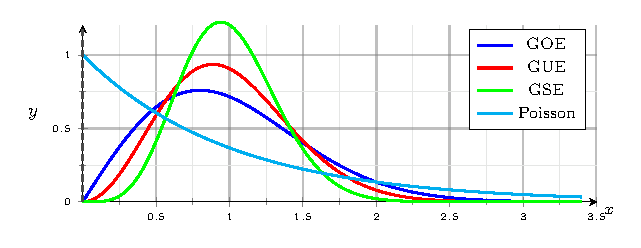
\includegraphics[scale=1,angle=0]{distributions.pdf}
    %\caption{Variabili $X_{n}$}

  %
  \noindent\\

  \decoRule
  \caption{Different distributions from Random Matrix Theory.}
  \label{fig:different_distributions}
\end{figure}


Quite remarkably, the distribution eigenvalues on the modular surface $X(1)=\PSL_{2}\Z$ follows a Poisson distribution (\cite{Rudnick:whatIs}).


\begin{figure}[H]
\centering

    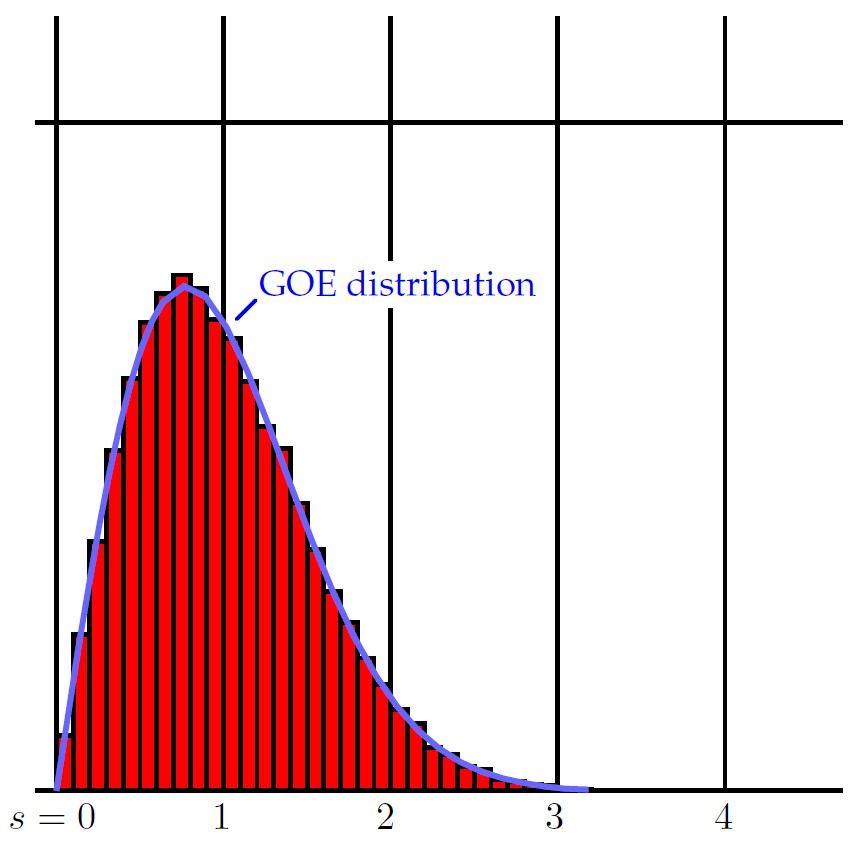
\includegraphics[scale=0.5,angle=0]{goe.jpg}
    %\caption{Variabili $X_{n}$}

  %
  \noindent\\

  \decoRule
  \caption{From \cite{Rudnick:whatIs}. Normalized gaps
between roughly 50000 sorted eigenvalues
for the Barnett's stadium \ref{fig:barnett_eigenfunction}. The distributions follows the \GOE distribution.}
  \label{fig:goe_distrib}
\end{figure}


On the contrary, the distribution is expected, by enormous numerical simulations by Odlyzko \cite{Odly:comput}, to follow the rare \GUE distribution (\cite{Rudnick:whatIs}).


\begin{figure}[H]
\centering

    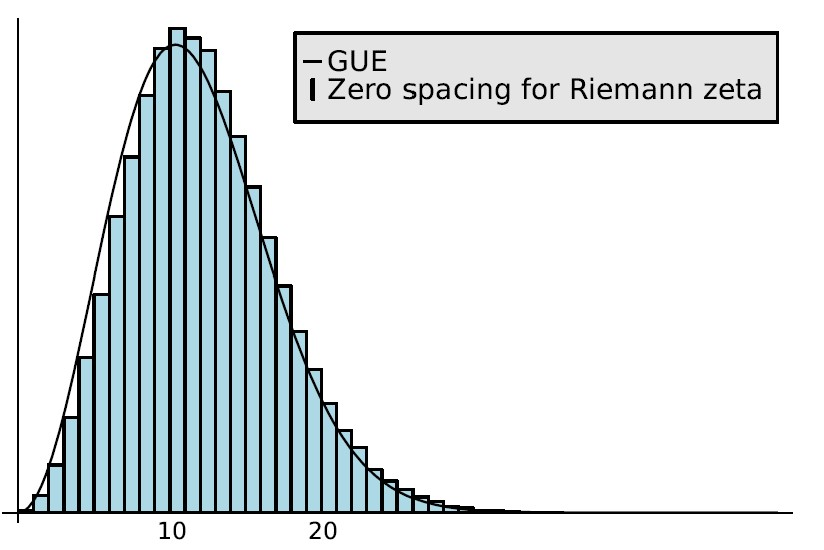
\includegraphics[scale=0.55,angle=0]{zeros_zeta_gue.jpg}
    %\caption{Variabili $X_{n}$}

  %
  \noindent\\

  \decoRule
  \caption{From \cite{Rudnick:whatIs}, computations by \cite{Odly:comput}. Distributions of zeros of Riemann zeta function.}
  \label{fig:gue_distrib_zeta}
\end{figure}



For further details, we refer to CITA. The hope of this approach is to increase the understanding about how integrable and chaotic systems differ in the semiclassical limit.










%----------------------------------------------------------------------------------------
%	SECTION 1
%----------------------------------------------------------------------------------------



\section{Conclusion}

To be done




\subsection{Billiard and spectral simulations}




%\include{Chapters/Chapter1}
%\include{Chapters/Chapter2} 
%\include{Chapters/Chapter3}
%\include{Chapters/Chapter4} 
%\include{Chapters/Chapter5}

%----------------------------------------------------------------------------------------
%	THESIS CONTENT - APPENDICES
%----------------------------------------------------------------------------------------

\appendix % Cue to tell LaTeX that the following "chapters" are Appendices

% Include the appendices of the thesis as separate files from the Appendices folder
% Uncomment the lines as you write the Appendices

% Appendix A

\chapter{Ergodic notions} % Main appendix title

\label{AppendixA} % For referencing this appendix elsewhere, use \ref{AppendixA}
\thispagestyle{empty}
%\section{Mixing}
%
%The color of links can be changed to your liking using:
%
%{\small\verb!\hypersetup{urlcolor=red}!}, or
%
%{\small\verb!\hypersetup{citecolor=green}!}, or
%
%{\small\verb!\hypersetup{allcolor=blue}!}.
%
%\noindent If you want to completely hide the links, you can use:
%
%{\small\verb!\hypersetup{allcolors=.}!}, or even better: 
%
%{\small\verb!\hypersetup{hidelinks}!}.
%
%\noindent If you want to have obvious links in the PDF but not the printed text, use:
%
%{\small\verb!\hypersetup{colorlinks=false}!}.


\section{Mixing}

In this section, we will prove theorem \ref{impTeo:mixing_flow_psl2}

\begin{nlem}
\label{lem:2.7_weakly_conv_invariant_phi_appendix}
If $\vphi\in\Hilb$ such that the sequence $\{\pi(A_{t_{n}})\vphi\}_{n\geq0}$ converges weakly to an element $\vphi_{0}$. Then $\vphi_{0}$ is itself invariant to the action of the group $\Lie{U}$.
\end{nlem}
\begin{prf}
Let $as$ Be simple matrix multiplications, we get 
\[
A_{-t}U_{s}A_{t}=U_{s\e^{-t}}.
\]
Then, for any $\psi\in H$,
\begin{align*}
\pscl{\pi(U_{s})\vphi_{0}-\vphi_{0}}{\psi}&=\lim_{n\to\infty}\pscl{\pi(U_{s}A_{t_{n}})\vphi-\pi(A_{t_{n}})\vphi}{\psi}\\
&=\lim_{n\to\infty}\pscl{\pi(A_{-t_{n}}U_{s}A_{t_{n}})\vphi-\vphi}{\pi(A_{-t_{n}})\psi}\\
&=\lim_{n\to\infty}\pscl{\pi(U_{s\e^{-t_{n}}})\vphi-\vphi}{\pi(A_{-t_{n}})\psi}\\
&\leq \lim_{n\to\infty}\norm{\pi(U_{s\e^{-t_{n}}})\vphi-\vphi}{\psi}
\end{align*}
where last inequality follows from Cauchy-Schwarz inequality and $U_{s\e^{-t_{n}}}\to I$. This concludes the proof.
\end{prf}


\begin{nlem}[Mautner phenomenon]
\label{lem:2.8_mautner_phenomemon_appendix}
If $\vphi\in\Hilb$ is invariant under the action of $U$, then it's invariant under $\SL_{2}\R$.
\end{nlem}
\begin{prf}
For any matrix $G\in\SL_{2}\R$, we define the function 
\[
F(G)=\pscl{\pi(G)\vphi}{\vphi}.
\]
Function $F$ is nothing else then a matrix coefficient METTI RIFERIMENTO. We note that $\vphi$ is bi-$U$-invariant. In fact:
\[
F(UGU')=\pscl{\pi(UGU')\vphi}{\vphi}=\pscl{\pi(G)\vphi}{\pi(U^{-1})\vphi}=F(G)\,\forall U,U'\in\Lie{U}.
\]
We consider the matrix
\[
B=\Matrix{1&r\\&1}\Matrix{1&\\\veps&1}\Matrix{1&s\\&1}=\Matrix{
1+\veps r& r+s+rs\veps\\
\veps & 1+s\veps
}.
\]
Let $r=(\e^{t}-1)/\veps$, for fixed $t\in\R,\veps>0$. So $B=\Smallmatrix{\e^{t}&\\\veps&\e^{-t}}$. This means that, for any $\veps,t>0$
\[
F\left(
\Matrix{1&\\\veps&1}\right)=F\left(
\Matrix{\e^{t}&\\\veps&\e^{-t}}
\right).
\]
By continuity of representation, if $\veps\to$, we have 
\[
\pscl{\vphi}{\vphi}=\lim_{\veps\to0}F(B)=F\left(
\Matrix{\e^{t}&\\&\e^{-t}}
\right).
\]
This means that $F(A_{t})=\pscl{\pi(A_{t})\vphi}{\vphi}=\norm{\vphi}^{2}$ and hence the equality case in Cauchy-Schwarz inequality holds. This is possible only if $\pi(A_{t})\vphi$ and $\vphi$ are linear dependent and but putting $t=0$, we get $\pi(A_{t})\vphi=\vphi$.  Using the same reasoning, it is possible to prove that $F$ is bi-$\Lie{A}$-invariant. In ana analogous way as before, we set 
\[
D=A_{-t}\Matrix{1&\\s\e^{-t}&1}A_{t}=\Matrix{1&\\s&1},
\]
to get that 
\[
F\left(
\Matrix{
1&\\
s\e^{-t}&1
}
\right)=F\left(
\Matrix{
1&\\
s&1
}
\right)
\]
Again, by a continuity argument, we get 
\[
F\left(
\Matrix{1&\\s&1}
\right)=\norm{\vphi}
\]
and thus the invariance of $\vphi$ under $\Lie{U}^{-}$. So $\vphi$ is invariant under the diagonal group $\Lie{A}$ and under the groups $\Lie{U}^{\pm}$, hence it must be invariant under the action of all group $\PSL_{2}\R$.
\end{prf}

We are now ready to prove the main result.

\begin{nteo}[Howe-Moore]
\label{teo:mixing_flow_psl2_appendix}
Let $\pi$ be a strongly continuos unitary representation of $\SL_{2}\R$ on a Hilbert space $\Hilb$. Assume that $\pi$ has non-trivial invariant vector in $\Hilb$. Then, if $G_{n}$ is a diverging\footnote{That is for any compact $K\subset \SL_{2}\R$, there exists $N\in\N$ such that $G_{n}\not\in K$ for all $n\geq N$.} sequence in $\SL_{2}\R$, then 
\[
\lim_{n\to\infty}\pscl{\pi(G_{n})\vphi}{\psi}=\int_{X}\vphi\dd\mu\int_{X}\psi\dd\mu
\]
\end{nteo}
\begin{prf}
As a first step, we will show that the converging thesis holds for the diagonal subgroup $\Lie{A}$. Suppose there exist $\vphi,\psi$ and a sequence $t_{n}\to\infty$ such that $ \pscl{\pi(A_{t_{n}})\vphi}{\psi}$ does not converge to $\int_{X}\vphi\dd\mu\int_{X}\psi\dd\mu$.\\
We have $\norm{\pi(A_{t_{n}})\vphi}=\norm{\vphi}$, so (by Banach-Alaoglu theorem) we can find a subsequence that is weakly convergent to some $\vphi_{0}$. By lemmas \ref{lem:2.7_weakly_conv_invariant_phi_appendix} and \ref{lem:2.8_mautner_phenomemon_appendix}, $\vphi_{0}$ is $\SL_{2}\R$-invariant, hence $\vphi_{0}$ is constant. This is a contradiction, because  the considered subsequence. Then, necessarily $\forall\phi,\psi\in H$, we have $\pscl{\pi(A_{t})}{\psi}\to\int_{X}\vphi\dd\mu\int_{X}\psi\dd\mu$ for $t\to\infty$.\\
For a general diverging sequence $G_{n}\in\SL_{2}\R$, there exists (for fixed $n$) $k_{n},k'_{n}\in\SO_{2}\R$ and a sequence $t_{n}\to\infty$ such that 
\[
G_{n}=K_{n}A_{t_{n}}K'_{n},\quad K_{n}, K_{n}'\in\SO_{2}\R.
\]
This is only a sort of \virg{hyperbolic-polar decomposition} of elements $G_{n}$. As $K_{n},K'_{n}$ are bounded elements in $\SL_{2}\R$, using multiple diagonal argument, we can choose a subsequence (which will be still denoted by index $n$) such that $K_{n}\to K$ and $K_{n}'\to K'$. So
\[
\pscl{\pi(G_{n})\vphi}{\psi}=\pscl{\pi(A_{t_{n}})\pi(K_{n}')\vphi}{\pi(K_{n})^{-1}\psi}
\]
has the same limit as
\[
\pscl{\pi(A_{t_{n}})\pi(K')\vphi}{\pi(K)^{-1}\psi}.
\]
However, the limit of this last term is $0$,

\end{prf}


% Appendix A

\chapter{Fourier transform} % Main appendix title

\label{Appendix_Fourier} % For referencing this appendix elsewhere, use \ref{AppendixA}
\thispagestyle{empty}

In this appendix we briefly review some notions and properties of the \emph{Fourier transform}.

\section{Basic notions}

We will present Fourier transform on $\R^{n}$, keeping in mind that it can be extended to general smooth manifolds using \emph{partition of unity}.\\

A suitable space for the Fourier transform is the so-called \emph{Schwarz space}, i.e. the space of \emph{rapidly decaying functions}. More precisely, we give the following definition, (\cite{Horm:book1})

\begin{defin}
\label{def:scwharz_space}
We define the seminorm $\norm{\cdot}_{\alpha,\beta}$ for a smooth function $f$ on $\R_{n}$ as 
\[
\norm{f}_{\alpha,\beta}\coloneqq\norm{x^{\alpha}\partial^{\beta}f}_{\infty}
\]
for fixed multiindices $\alpha\in\N^{n}$ and $\beta$, where\footnote{We are implicitly using the fact that the derivatives commute.}
\[
x^{\alpha}=\prod_{i}^{n}x_{i}^{\alpha_{i}},\quad\partial^{\beta}=\prod_{i=1}^{n}\partial_{x_{i}^{\beta_{i}}}.
\]
The \emph{Schwarz space} (in $\R^{n}$) is the set $\schwarz=\schwarz(\R^{n})=\left\{f\in C^{\infty}(\R^{n})\colon\norm{f}_{\alpha,\beta}<\infty\;\forall\alpha,\beta\in\N^{n}\right\}$. The space $(\schwarz,\norm{\cdot}_{\alpha,\beta})$ is a Fréchet space over $\mathbb{C}$ and we say $f_{j}\to f$ in $\schwarz$ if $\norm{f_{j}-f}_{\alpha,\beta}\to 0$ for all multiindices $\alpha,\beta$. 
\end{defin}


\begin{defin}
\label{def:Four_transform}
The Fourier is defined by $\Fourier\colon\schwarz\ni f\mapsto\Four{f}\in\schwarz$ (we will also use the notation $\hat{f}$ for the Fourier transform of $f$) and 
\[
\Four{f}(p)=\int_{\R^{n}}\e^{-\imi\pscl{p}{x}}f(x)\dd x,
\]
with the inverse given by
\[
\Fourier^{-1}(f)(x)=\frac{1}{(2\pi)^{n}}\int_{\R^{n}}\e^{\imi\pscl{x}{p}}f(p)\dd p.
\]
\end{defin}

The Fourier transform can be defined also for larger spaces, see for example Plancherel theorem. A useful result is the following.

\begin{nlem}
Let be given a real, symmetric and positive-definite quadratic form $x^{\trsp}Qx$, where $Q$ is a $n\times n$-matrix. Then
\[
\Fourier\left(\e^{-\frac{1}{2}x^{\trsp}Qx}\right)=\frac{(2\pi)^{n/2}}{(\det Q)^{1/2}}\e^{-\frac{1}{2}\pscl{Q^{-1}p}{p}}.
\]
\end{nlem}
\begin{prf}
Using the spectral theorem, we can choose an orthogonal basis $v_{1},\ldots, v_{n}$ for $\R^{n}$ that makes $Q$ diagonal, with diagonal elements $\lambda_{1}^{2},\ldots,\lambda_{n}^{2}$, where each element is positive. Hence, if $A$ is the coordinate-change matrix and $D=\diag(\lambda_{1}^{2},\ldots,\lambda_{n}^{2})$, using Einstein notation, from a straightforward computation we get that
\begin{align*}
\Fourier(\e^{-\frac{1}{2}x^{\trsp}Qx})&=\int_{\R_{n}}\e^{-\frac{1}{2}\left(\lambda_{i}^{2}v_{i}^{2}-2\imi v_{i}(a_{ji}p_{j})-\frac{(a_{ji}p_{j})}{\lambda_{i}^{2}}\right)-\frac{1}{2}\frac{(a_{ji}p_{j})^{2}}{\lambda_{i}^{2}}}\dd v\\
&=\e^{-\frac{1}{2}\frac{(a_{ji}p_{j})^{2}}{\lambda_{i}^{2}}}\int_{\R^{n}}\e^{-\frac{1}{2}\left(\lambda_{i}v_{i}-\imi\frac{(a_{ji}p_{j})}{\lambda_{i}}\right)^{2}}\dd v.
\end{align*}
The external term $\e^{-\frac{1}{2}\frac{(a_{ji}p_{j})^{2}}{\lambda_{i}^{2}}}$ can be seen as $\pscl{AD^{-1}A^{\trsp}p}{p}$. But, from $A^{\trsp}Q A=D$, we get that $Q^{-1}=AD^{-1}A^{\trsp}$, hence we get $\e^{-\frac{1}{2}\pscl{Q^{-1}p}{p}}$. The integral part and can be computed by separating each $v_{i}$ and using the substitution $y_{i}=\lambda_{i}v_{i}-\imi\frac{(a_{ji}p_{j})}{\lambda_{i}}$ we get standard guassian integral. The final result is 
\[
\e^{-\frac{1}{2}\frac{(a_{ji}p_{j})^{2}}{\lambda_{i}^{2}}}\int_{\R^{n}}\e^{-\frac{1}{2}\left(\lambda_{i}v_{i}-\imi\frac{(a_{ji}p_{j})}{\lambda_{i}}\right)^{2}}\dd v=\e^{-\frac{1}{2}\frac{(a_{ji}p_{j})^{2}}{\lambda_{i}^{2}}}\prod_{i=1}^{n}\frac{(2\pi)^{1/2}}{\lambda_{i}}=\frac{(2\pi)^{n/2}}{(\det Q)^{1/2}}\e^{-\frac{1}{2}\frac{(a_{ji}p_{j})^{2}}{\lambda_{i}^{2}}},
\]
and we are done.
\end{prf}


The main properties of the Fourier transform are summarized by the following.


\begin{nprop}
\label{prop:four_properties}
The Fourier transform $\Fourier\colon\schwarz\to\schwarz$ is an isomorphism of topological vector spaces. Moreover, for all $f,g\in\schwarz$ hold:
\begin{compactenum}
\item $\Diff^{\alpha}_{p}(\Fourier(f))=\Fourier((-x)^{\alpha}f)$ and $\Fourier(\Diff_{x}^{\alpha}(f))=p^{\alpha}\Fourier(f)$, where $\Diff_{x}^{\alpha}\coloneqq\frac{\partial^{\alpha}}{\imi^{\abs{\alpha}}}$.
\item $\Fourier(f\ast g)=(2\pi)^{-n}\Fourier(f)\ast\Fourier(g)$, where $\ast$ is the standard convolution.
\item $\pscl{\Fourier(f)}{g}=\pscl{f}{\Fourier(g)}$.
\item the Fourier transform is an $L^{2}$-isometry.
\end{compactenum}
\end{nprop}


\section{Distributions}


Another tool linked to the Fourier transform is the notion of \emph{distribution}. In general, a \emph{distribution} on $\R^{n}$ is a linear functional $\vphi\colon C_{c}^{\infty}(\R^{n})\to\R$ such that $\vphi(f_{n})\to\vphi(f)$, if $f_{n}\to f$ with the respect to the previously introduced seminorm, in $C_{c}^{\infty}(\R^{n})$. The set of all distributions generalizes and forms a vector space dual to $C_{c}^{\infty}(\R^{n})$. Often, the distribution are improperly denoted by some functions, when they are actually applications.\\
The vector space of tempered distributions $\schwarz'$ is defined by duality from the Schwartz space $\schwarz$. Introducing tempered distributions gives, among other things, the correct vector space for a rigorous formulation of the Fourier transforms of nonsmooth functions. 

\begin{defin}
\label{def:tempered_distrib}
Let the space of tempered distributions $\schwarz'$ be the set of all continuos linear functionals $\vphi\colon\schwarz\ni f\mapsto\vphi(f)$. We say that $\vphi_{j}\rightharpoonup\vphi$ in $\schwarz'$ if there the convergence componentwise (i.e. for each function $f\in\schwarz$). Moreover, we define, for each multiindex $\alpha\in\N^{n}$:
\begin{compactitem}
\item $\Diff^{\alpha}\vphi(f)\coloneqq (-1)^{\abs{\alpha}}\vphi(\Diff^{\alpha}f)$.
\item $(x^{\alpha}\vphi)(f)\coloneqq\vphi(x^{\alpha} f)$.
\end{compactitem} 
Finally, $\Fourier$ extends to $\schwarz'$ by setting $\Fourier(\vphi)(f)\coloneqq\vphi(\Fourier(f))$, $\forall\vphi\in\schwarz',f\in\schwarz$.
\end{defin}

\begin{nese}[Fourier transform of Dirac distribution]
The Dirac distribution is defined by $\delta_{0}(f)=f(0)$. Viewed as a tempered distribution, its Fourier transform is 
\[
\Fourier(\delta_{0})(f)=\delta_{0}\Fourier(f)=Fourier(f)(0)=1.
\]
\end{nese}


Using distributions, it is possible to prove the following result. We omit the proof, as it is a little involved.

\begin{nprop}
\label{prop:Fourier_imaginiary}
Let be given a real, symmetric and invertible quadratic form $x^{\trsp}Qx$, where $Q$ is a $n\times n$-matrix. Then
\[
\Fourier\left(\e^{-\frac{1}{2}\imi x^{\trsp}Qx}\right)=\frac{(2\pi)^{n/2}\e^{\imi\frac{\pi}{4}\sgn Q}}{\abs{\det Q}^{1/2}}\e^{-\frac{1}{2}\imi\pscl{Q^{-1}p}{p}}.
\]
where $\sgn Q$ is the \emph{signature} of $Q$. 
\end{nprop}














% Appendix A

\chapter{Flows and integrable systems} % Main appendix title

\label{AppendixC} % For referencing this appendix elsewhere, use \ref{AppendixA}
\thispagestyle{empty}

\section{Ergodic notions}




\begin{nteo}
\label{teo:weak_birhoff_theorem}
If $\Phi_{t}$ is ergodic on $(\Sigma_{c},\chi,\mu_{L}^{c})$, then
\[
\lim_{T\to\infty}\int_{\Sigma_{c}}\left(\spn{f}_{T}-\fint_{\Sigma_{c}}f\dd\mu_{L}^{c}\right)^{2}\dd\mu_{L}^{c}=0,
\]
for all $f\in L^{2}(\Sigma_{c})$, where $\fint$ denotes the mean integral.
\end{nteo}



\begin{nteo}[Birkhof's theorem]
\label{nteo:weak_birhoff_theorem}
If $\Phi_{t}$ is ergodic on $(\Sigma_{c},\chi,\mu_{L}^{c})$, then...
\end{nteo}

METTERE HOPF 
%\include{Appendices/AppendixD}
% Appendix Template

%\chapter{Source Code for Figures and Numerical Simulations} % Main appendix title

\label{App:codes} % Change X to a consecutive letter; for referencing this appendix elsewhere, use \ref{AppendixX}


\lstlistoflistings

\section{Python codes}

\subsection{Billiards}

Put your Codes here.

\lstinputlisting[language=Python, caption={Billiard simulation in Bunimovich stadium},label={pycode:image_bunimov}, mathescape=true]{codes_thesis/Python/image_stadium_billiard.py}

%\begin{lstlisting}[language=Python, caption={Stadium},label={pycode:stadium},mathescape=true, breaklines=true]
%
%def getTragectory(p,v): # p is the position, v is the velocity vector
%    #xc=x+y*m
%    return [p,v] #[xc,0,math.sqrt((xc-x)**2+y**2)]
%
%def bounce_circle(direction, b_point, center):
%    """
%    Calculate the new direction after a bouncing with a circled wall
%    """
%    F1 = [[b_point[0]-center[0], b_point[1]-center[1]], [b_point[1]-center[1], center[0]-b_point[0]]]
%    F2 = [[-1, 0], [0, 1]]
%    F3 = [[center[0]-b_point[0],center[1]-b_point[1]],[-(b_point[1]-center[1]),b_point[0]-center[0]]]
%    #F3 = [[b_point[0]-center[0],b_point[1]-center[1]],[-b_point[1]+center[1],-b_point[0]+center[0]]]
%    F3 = -np.dot(1/((b_point[0]-center[0])**2+(b_point[1]-center[1])**2), F3)
%    return np.dot(np.matmul(np.matmul(F1, F2), F3), direction)
%
%#print("prova:", np.dot([[0,1],[-1,0]],[2,3]))
%#print("nuova direzione", bounce_circle([1,1],[np.sqrt(Radius)+WIDTH/2,np.sqrt(Radius)],[WIDTH/2,0]))
%
%
%def upper_wall_intersection(p,v,Radius):
%    l, r = 0, INF
%    while r-l > EPS:
%        m = (l+r)/2
%        if p[1]+m*v[1] > Radius:
%            r = m
%        else:
%            l = m
%    return l
%
%
%\end{lstlisting}


\subsection{Quantum eigenfunctions}



\section{FreeFem++}


\lstinputlisting[language=freefem++, caption={Eigenfunctions of modular surface},label={FreeFem:modular_eig_D}, mathescape=true]{codes_thesis/FreeFem++/modular.edp}




%% Appendix A

\chapter{Flows and integrable systems} % Main appendix title

\label{AppendixC} % For referencing this appendix elsewhere, use \ref{AppendixA}
\thispagestyle{empty}

\section{Ergodic notions}




\begin{nteo}
\label{teo:weak_birhoff_theorem}
If $\Phi_{t}$ is ergodic on $(\Sigma_{c},\chi,\mu_{L}^{c})$, then
\[
\lim_{T\to\infty}\int_{\Sigma_{c}}\left(\spn{f}_{T}-\fint_{\Sigma_{c}}f\dd\mu_{L}^{c}\right)^{2}\dd\mu_{L}^{c}=0,
\]
for all $f\in L^{2}(\Sigma_{c})$, where $\fint$ denotes the mean integral.
\end{nteo}



\begin{nteo}[Birkhof's theorem]
\label{nteo:weak_birhoff_theorem}
If $\Phi_{t}$ is ergodic on $(\Sigma_{c},\chi,\mu_{L}^{c})$, then...
\end{nteo}

METTERE HOPF 


%----------------------------------------------------------------------------------------
%	LIST OF FIGURES/TABLES PAGES
%----------------------------------------------------------------------------------------


\listoffigures % Prints the list of figures

%\listoftables % Prints the list of tables


%----------------------------------------------------------------------------------------
%	BIBLIOGRAPHY
%----------------------------------------------------------------------------------------
\begingroup
\setlength\bibitemsep{8pt} 
\setstretch{1}
\nocite{*}
\printbibliography[heading=bibintoc]
\endgroup


%----------------------------------------------------------------------------------------

\end{document}  
